% =============================================================================
%  slides.tex (docs/presentation7): RISC-V vector (RVV) code generation in pystencils and waLBerla for
%  128- and 256-bit vectors, measured on two machines: the SpacemiT K1 (VLEN 256) and the Sophgo SG2044 on
%  Monte Cimone (VLEN 128). About 25-30 minutes, for listeners who know software but not this project.
%  Based on docs/presentation6 (which is presentation5: K1 only). Build with ./build.sh (build/slides.pdf).
%
%  Structure (presentation7-v3, user, 2026-11-25): three main sections. (1) The lattice Boltzmann method: every
%  background slide on the method and its memory traffic (test case, stencil, f_i and f'_i, storage, ghost layer and
%  halo exchange, time step, streams, AA and AB, split loop, the update in code). (2) Our work: RVV support for the K1
%  and the SG2044 (build chain, what we added, the width check, both machines' hardware, the stream limit and
%  software prefetch). (3) Results (correctness and protocol, K1, SG2044, the two machines compared). Then Summary
%  and the backup. Every section starts with the overview slide: the current section in colour with its
%  subsections indented, the others in grey (\AtBeginSection, \overviewframe).
%  (presentation7-v2 had: Background, Code for two vector widths, The kernel, Part 1 K1, Part 2 SG2044, Both
%  machines, Summary.)
%
%  Sources of every number: tables/ (written by scripts/presentation7/slide_data.py, which checks the logs
%  first; each table names its source logs and their sha256). Result numbers in the text are \nv{key} from
%  tables/numbers.tex, never typed in. The script also stops if a statement the text makes in words (which build
%  is faster, a tie, a direction) no longer holds. Typed-in numbers are only: hardware facts, the protocol
%  constants, and the K1 probe and lab numbers that presentation6 already showed (their sources are in the
%  comments of the figures and frames, copied from presentation6). K1 logs: board-logs/k1/ (copies of
%  docs/presentation6/board-logs/). SG2044 logs: 00_private_data/monte3/20261122-214637/ (private, not
%  committed; jobs 8565 and 8566). Progress and checks: presentation7-progress-opus5.5.md.
%
%  Writing rules: simple English in full sentences, at most about four bullets per slide, one short takeaway,
%  details in the grey note or the backup; every name explained where it first appears and in the glossary.
% =============================================================================
\documentclass[aspectratio=169,10pt,t]{beamer}

\usepackage[T1]{fontenc}
\usepackage[utf8]{inputenc}
\usepackage[sfdefault,lining]{FiraSans}
\usepackage[varqu]{inconsolata}
\usefonttheme{professionalfonts}
\usepackage{amsmath,amssymb}
\usepackage{booktabs,array,tabularx}
\usepackage{pifont}
\usepackage{catchfile}   % the full tables are read into a macro (\input inside tabular breaks \bottomrule)
\usepackage{appendixnumberbeamer}

\usepackage{tikz}
\usetikzlibrary{positioning,arrows.meta,calc,fit,backgrounds,decorations.pathreplacing,patterns}
\usepackage{pgfplots}
\usepgfplotslibrary{groupplots}
\usepackage{pgfplotstable}
\usepackage{multimedia}   % the flow films: \movie links figures/cavity-movie*/cavity.avi (played by pdfpc)
\pgfplotsset{compat=1.18}
\pgfkeys{/pgf/number format/assume math mode=true,/pgf/number format/1000 sep={}}   % numbers in plots in the text font (Fira), not in math font
\pgfplotstableset{comment chars={\%}}   % tables/*.dat start with a header of source logs

% ---- Numbers from tables/numbers.tex --------------------------------------------------
%   \nv{key}: a number written by scripts/presentation7/slide_data.py; an unknown key stops the build.
\newcommand{\nset}[2]{\expandafter\def\csname nv@#1\endcsname{#2}}
\newcommand{\nv}[1]{\ifcsname nv@#1\endcsname\csname nv@#1\endcsname\else
  \errmessage{presentation7: unknown number '#1' (see tables/numbers.tex)}\fi}
% written by scripts/presentation7/slide_data.py; do not edit by hand
% SG2044 run 20261122-214637
% source 9c353b8f8238af08 docs/presentation7/board-logs/k1/board/ldc-gcc-scalar-f32-1core.log
% source d919d426ead826fd docs/presentation7/board-logs/k1/board/ldc-gcc-autovec-f32-1core.log
% source 5ddea86544f3bfa5 docs/presentation7/board-logs/k1/board/ldc-gcc-rvv-f32-1core.log
% source 71647774850a0554 docs/presentation7/board-logs/k1/board/ldc-gcc-scalar-f32-4core.log
% source cc25932787802d7f docs/presentation7/board-logs/k1/board/ldc-gcc-autovec-f32-4core.log
% source 4c1a7e2567aea7f2 docs/presentation7/board-logs/k1/board/ldc-gcc-rvv-f32-4core.log
% source 0d5ee8fadfcc0c60 docs/presentation7/board-logs/k1/board/ldc-gcc-scalar-f32-8core.log
% source ec4dce60813e50f3 docs/presentation7/board-logs/k1/board/ldc-gcc-autovec-f32-8core.log
% source 9c45f588f0c78f12 docs/presentation7/board-logs/k1/board/ldc-gcc-rvv-f32-8core.log
% source 84313f628e655ae8 docs/presentation7/board-logs/k1/board/ldc-gcc-scalar-f64-1core.log
% source 84193137e008fd7e docs/presentation7/board-logs/k1/board/ldc-gcc-autovec-f64-1core.log
% source 09db3b14734d5800 docs/presentation7/board-logs/k1/board/ldc-gcc-rvv-f64-1core.log
% source 82b58890093873bf docs/presentation7/board-logs/k1/board/ldc-gcc-scalar-f64-4core.log
% source cf354173e2a137ee docs/presentation7/board-logs/k1/board/ldc-gcc-autovec-f64-4core.log
% source a79e6be8a4ba9768 docs/presentation7/board-logs/k1/board/ldc-gcc-rvv-f64-4core.log
% source 0b1573e24c0054af docs/presentation7/board-logs/k1/board/ldc-gcc-scalar-f64-8core.log
% source 96fb4995d04eda72 docs/presentation7/board-logs/k1/board/ldc-gcc-autovec-f64-8core.log
% source d966f1714e72fb30 docs/presentation7/board-logs/k1/board/ldc-gcc-rvv-f64-8core.log
% source 685927922a50b6c4 docs/presentation7/board-logs/k1/board/ldc-clang-scalar-f32-1core.log
% source d432730248cee74c docs/presentation7/board-logs/k1/board/ldc-clang-autovec-f32-1core.log
% source 5da9f642d6b52c8d docs/presentation7/board-logs/k1/board/ldc-clang-rvv-f32-1core.log
% source ca1e00a73d68bde5 docs/presentation7/board-logs/k1/board/ldc-clang-scalar-f32-4core.log
% source 99f10b72116b143d docs/presentation7/board-logs/k1/board/ldc-clang-autovec-f32-4core.log
% source 833c26f5b34397ee docs/presentation7/board-logs/k1/board/ldc-clang-rvv-f32-4core.log
% source f567f8a6ad26e9f9 docs/presentation7/board-logs/k1/board/ldc-clang-scalar-f32-8core.log
% source efbe4a69a42d7b02 docs/presentation7/board-logs/k1/board/ldc-clang-autovec-f32-8core.log
% source 9443864ade46d03b docs/presentation7/board-logs/k1/board/ldc-clang-rvv-f32-8core.log
% source b32253399d30d932 docs/presentation7/board-logs/k1/board/ldc-clang-scalar-f64-1core.log
% source 2a44dae4a3e86585 docs/presentation7/board-logs/k1/board/ldc-clang-autovec-f64-1core.log
% source fd62e2395405401d docs/presentation7/board-logs/k1/board/ldc-clang-rvv-f64-1core.log
% source 9ded76986176e231 docs/presentation7/board-logs/k1/board/ldc-clang-scalar-f64-4core.log
% source 2a957f6d3fc7dded docs/presentation7/board-logs/k1/board/ldc-clang-autovec-f64-4core.log
% source b8b3bc6355dde063 docs/presentation7/board-logs/k1/board/ldc-clang-rvv-f64-4core.log
% source 562100697c16227f docs/presentation7/board-logs/k1/board/ldc-clang-scalar-f64-8core.log
% source 13b722b3185a00e8 docs/presentation7/board-logs/k1/board/ldc-clang-autovec-f64-8core.log
% source f7c4a2565b9896ef docs/presentation7/board-logs/k1/board/ldc-clang-rvv-f64-8core.log
% source b3bdfd929d9e6b1d 00_private_data/monte3/20261122-214637/ldc-gcc-scalar-f32-1core.log
% source 264fe94b446cd03a 00_private_data/monte3/20261122-214637/ldc-gcc-autovec-f32-1core.log
% source 459fa6b94ebe5e95 00_private_data/monte3/20261122-214637/ldc-gcc-rvv-f32-1core.log
% source a9e94ab155ae7617 00_private_data/monte3/20261122-214637/ldc-gcc-scalar-f32-4core.log
% source a53481eb6d6d8e69 00_private_data/monte3/20261122-214637/ldc-gcc-autovec-f32-4core.log
% source c04c3e74ca1ebcde 00_private_data/monte3/20261122-214637/ldc-gcc-rvv-f32-4core.log
% source 95be91ba2d880016 00_private_data/monte3/20261122-214637/ldc-gcc-scalar-f32-8core.log
% source 89b0c45992c4e445 00_private_data/monte3/20261122-214637/ldc-gcc-autovec-f32-8core.log
% source e8ec9b2c01375df4 00_private_data/monte3/20261122-214637/ldc-gcc-rvv-f32-8core.log
% source 521b50a13c009c69 00_private_data/monte3/20261122-214637/ldc-gcc-scalar-f32-16core.log
% source 7c3c4230d8b4ecf3 00_private_data/monte3/20261122-214637/ldc-gcc-autovec-f32-16core.log
% source 731da62bda96b370 00_private_data/monte3/20261122-214637/ldc-gcc-rvv-f32-16core.log
% source 5191b4ce38140bb4 00_private_data/monte3/20261122-214637/ldc-gcc-scalar-f32-32core.log
% source 622243d1c51c1862 00_private_data/monte3/20261122-214637/ldc-gcc-autovec-f32-32core.log
% source 3304a5054449c25a 00_private_data/monte3/20261122-214637/ldc-gcc-rvv-f32-32core.log
% source 627a077386782779 00_private_data/monte3/20261122-214637/ldc-gcc-scalar-f32-64core.log
% source 6446d66d7c75b045 00_private_data/monte3/20261122-214637/ldc-gcc-autovec-f32-64core.log
% source 002bcedd5130dd25 00_private_data/monte3/20261122-214637/ldc-gcc-rvv-f32-64core.log
% source 4e9f25f715bd7e87 00_private_data/monte3/20261122-214637/ldc-gcc-scalar-f64-1core.log
% source 0d01d2384edb3a8f 00_private_data/monte3/20261122-214637/ldc-gcc-autovec-f64-1core.log
% source 83d1f2206f6ec82d 00_private_data/monte3/20261122-214637/ldc-gcc-rvv-f64-1core.log
% source 5e9ce63c241d665c 00_private_data/monte3/20261122-214637/ldc-gcc-scalar-f64-4core.log
% source 1690c2b8885359e2 00_private_data/monte3/20261122-214637/ldc-gcc-autovec-f64-4core.log
% source ebf3dd87c4cfd178 00_private_data/monte3/20261122-214637/ldc-gcc-rvv-f64-4core.log
% source 5219e477d8b3fb4b 00_private_data/monte3/20261122-214637/ldc-gcc-scalar-f64-8core.log
% source 12fbfffa22c01676 00_private_data/monte3/20261122-214637/ldc-gcc-autovec-f64-8core.log
% source 46ff6778925a9f40 00_private_data/monte3/20261122-214637/ldc-gcc-rvv-f64-8core.log
% source 85811bfb463b80c1 00_private_data/monte3/20261122-214637/ldc-gcc-scalar-f64-16core.log
% source eddbc4ada0fca013 00_private_data/monte3/20261122-214637/ldc-gcc-autovec-f64-16core.log
% source 0c8d70b1799f74d2 00_private_data/monte3/20261122-214637/ldc-gcc-rvv-f64-16core.log
% source e8d1b8b80600e86f 00_private_data/monte3/20261122-214637/ldc-gcc-scalar-f64-32core.log
% source 366b7a00a0c00633 00_private_data/monte3/20261122-214637/ldc-gcc-autovec-f64-32core.log
% source 64bbefadfa03731e 00_private_data/monte3/20261122-214637/ldc-gcc-rvv-f64-32core.log
% source 1eb9da404175dfa7 00_private_data/monte3/20261122-214637/ldc-gcc-scalar-f64-64core.log
% source 2c69b5ac6fe6fddb 00_private_data/monte3/20261122-214637/ldc-gcc-autovec-f64-64core.log
% source fa7753bd051a516d 00_private_data/monte3/20261122-214637/ldc-gcc-rvv-f64-64core.log
% source 591a4bd0173adf5d 00_private_data/monte3/20261122-214637/ldc-clang-scalar-f32-1core.log
% source 6f5a61f9845c2a41 00_private_data/monte3/20261122-214637/ldc-clang-autovec-f32-1core.log
% source 123542f6ee7f139c 00_private_data/monte3/20261122-214637/ldc-clang-rvv-f32-1core.log
% source f60dac6fc8b80b2f 00_private_data/monte3/20261122-214637/ldc-clang-scalar-f32-4core.log
% source b54667e35cdba571 00_private_data/monte3/20261122-214637/ldc-clang-autovec-f32-4core.log
% source 0a9d32ef58a3266c 00_private_data/monte3/20261122-214637/ldc-clang-rvv-f32-4core.log
% source e10768ba823baa1e 00_private_data/monte3/20261122-214637/ldc-clang-scalar-f32-8core.log
% source 31d41e3cb34bbac8 00_private_data/monte3/20261122-214637/ldc-clang-autovec-f32-8core.log
% source 7e72614dd10e9fee 00_private_data/monte3/20261122-214637/ldc-clang-rvv-f32-8core.log
% source b5fff596b860d459 00_private_data/monte3/20261122-214637/ldc-clang-scalar-f32-16core.log
% source 3b39d14dd3d57a70 00_private_data/monte3/20261122-214637/ldc-clang-autovec-f32-16core.log
% source 305d8dd363b08938 00_private_data/monte3/20261122-214637/ldc-clang-rvv-f32-16core.log
% source 2977d049ace4dda6 00_private_data/monte3/20261122-214637/ldc-clang-scalar-f32-32core.log
% source cea3fa35d6bc59ed 00_private_data/monte3/20261122-214637/ldc-clang-autovec-f32-32core.log
% source 37d283adf7397c42 00_private_data/monte3/20261122-214637/ldc-clang-rvv-f32-32core.log
% source 68be6ea40fe002b3 00_private_data/monte3/20261122-214637/ldc-clang-scalar-f32-64core.log
% source f57c9a89b1021734 00_private_data/monte3/20261122-214637/ldc-clang-autovec-f32-64core.log
% source 2ecf4bac118bc6f0 00_private_data/monte3/20261122-214637/ldc-clang-rvv-f32-64core.log
% source 9129f56b87c55216 00_private_data/monte3/20261122-214637/ldc-clang-scalar-f64-1core.log
% source 64883c9b22139cf2 00_private_data/monte3/20261122-214637/ldc-clang-autovec-f64-1core.log
% source 62ef7e7aac9dbbb5 00_private_data/monte3/20261122-214637/ldc-clang-rvv-f64-1core.log
% source e6bcbfc5a052b37e 00_private_data/monte3/20261122-214637/ldc-clang-scalar-f64-4core.log
% source e69270907da9110d 00_private_data/monte3/20261122-214637/ldc-clang-autovec-f64-4core.log
% source 24669a3764a5408f 00_private_data/monte3/20261122-214637/ldc-clang-rvv-f64-4core.log
% source cb6b8ed6ef2fd69c 00_private_data/monte3/20261122-214637/ldc-clang-scalar-f64-8core.log
% source a9f7122fe5f3be18 00_private_data/monte3/20261122-214637/ldc-clang-autovec-f64-8core.log
% source 4c4f7be2c10e6404 00_private_data/monte3/20261122-214637/ldc-clang-rvv-f64-8core.log
% source cdda73e959b5e69a 00_private_data/monte3/20261122-214637/ldc-clang-scalar-f64-16core.log
% source c2c9ca5cdc83d491 00_private_data/monte3/20261122-214637/ldc-clang-autovec-f64-16core.log
% source 97164ab80add5b3d 00_private_data/monte3/20261122-214637/ldc-clang-rvv-f64-16core.log
% source 26492b34f0789a86 00_private_data/monte3/20261122-214637/ldc-clang-scalar-f64-32core.log
% source 905a303d824d2b5d 00_private_data/monte3/20261122-214637/ldc-clang-autovec-f64-32core.log
% source d6d621e0b29c2b11 00_private_data/monte3/20261122-214637/ldc-clang-rvv-f64-32core.log
% source 82c74b3b12b1e4d5 00_private_data/monte3/20261122-214637/ldc-clang-scalar-f64-64core.log
% source ca5a0fcffc8a4c63 00_private_data/monte3/20261122-214637/ldc-clang-autovec-f64-64core.log
% source af7f0ed1759cafba 00_private_data/monte3/20261122-214637/ldc-clang-rvv-f64-64core.log
% source 3a05348b72345fef docs/presentation7/board-logs/k1/board/verify-gcc-f32.log
% source 68c2622c5a199629 docs/presentation7/board-logs/k1/board/verify-gcc-f64.log
% source ca30c0b76ebbdaff docs/presentation7/board-logs/k1/board/verify-clang-f32.log
% source 430320486754524f docs/presentation7/board-logs/k1/board/verify-clang-f64.log
% source 24f257ff96a91530 00_private_data/monte3/20261122-214637/verify-gcc-f32.log
% source 74461e6ce0864ed4 00_private_data/monte3/20261122-214637/verify-gcc-f64.log
% source b009534464b0e54b 00_private_data/monte3/20261122-214637/verify-clang-f32.log
% source e00524fd0d5b8b0d 00_private_data/monte3/20261122-214637/verify-clang-f64.log
% source 8c28c5986386b87c 00_private_data/monte3/20261122-214637/build-8565.out
% source 1cb42e9411523be8 00_private_data/monte3/20261122-214637/time-8566.out
% source 7b0f4f12a6edd43c docs/presentation7/board-logs/k1/notes5/e2-A-output-last.log
% source 5e0578deddc12edf docs/presentation7/board-logs/k1/notes5/e10-A-clang-output-last.log
% source 003700cbbfbd405d 00_private_data/monte3/20261122-214637/share-gcc-f32-every.log
% source 0a2dda1189158b88 00_private_data/monte3/20261122-214637/share-gcc-f32-last.log
% source 349d420e127044ed 00_private_data/monte3/20261122-214637/share-gcc-f64-every.log
% source 949be1d16f3dece6 00_private_data/monte3/20261122-214637/share-gcc-f64-last.log
% source 086b346135fae201 00_private_data/monte3/20261122-214637/share-clang-f32-every.log
% source 1a73492e096629d4 00_private_data/monte3/20261122-214637/share-clang-f32-last.log
% source 1f2a578294a76794 00_private_data/monte3/20261122-214637/share-clang-f64-every.log
% source bf01c83fb179bb26 00_private_data/monte3/20261122-214637/share-clang-f64-last.log

\nset{kone:autovecdiff}{1.8}
\nset{kone:autovecgain}{1.8}
\nset{kone:clang/gcc:f32:1:aa}{1.00}
\nset{kone:clang/gcc:f32:1:aapf}{0.94}
\nset{kone:clang/gcc:f32:1:best}{1.05}
\nset{kone:clang/gcc:f32:1:bestav}{1.04}
\nset{kone:clang/gcc:f32:1:cse}{1.07}
\nset{kone:clang/gcc:f32:1:cseav}{1.07}
\nset{kone:clang/gcc:f32:1:pf}{0.92}
\nset{kone:clang/gcc:f32:1:plain}{0.98}
\nset{kone:clang/gcc:f32:1:plainav}{0.98}
\nset{kone:clang/gcc:f32:1:rvv}{0.95}
\nset{kone:clang/gcc:f32:1:split}{0.98}
\nset{kone:clang/gcc:f32:4:aa}{0.98}
\nset{kone:clang/gcc:f32:4:aapf}{0.96}
\nset{kone:clang/gcc:f32:4:best}{1.05}
\nset{kone:clang/gcc:f32:4:bestav}{1.05}
\nset{kone:clang/gcc:f32:4:cse}{1.06}
\nset{kone:clang/gcc:f32:4:cseav}{1.06}
\nset{kone:clang/gcc:f32:4:pf}{0.96}
\nset{kone:clang/gcc:f32:4:plain}{0.99}
\nset{kone:clang/gcc:f32:4:plainav}{0.99}
\nset{kone:clang/gcc:f32:4:rvv}{0.98}
\nset{kone:clang/gcc:f32:4:split}{0.98}
\nset{kone:clang/gcc:f32:8:aa}{0.98}
\nset{kone:clang/gcc:f32:8:aapf}{0.97}
\nset{kone:clang/gcc:f32:8:best}{1.03}
\nset{kone:clang/gcc:f32:8:bestav}{1.03}
\nset{kone:clang/gcc:f32:8:cse}{1.03}
\nset{kone:clang/gcc:f32:8:cseav}{1.03}
\nset{kone:clang/gcc:f32:8:pf}{0.96}
\nset{kone:clang/gcc:f32:8:plain}{0.97}
\nset{kone:clang/gcc:f32:8:plainav}{0.99}
\nset{kone:clang/gcc:f32:8:rvv}{0.98}
\nset{kone:clang/gcc:f32:8:split}{0.99}
\nset{kone:clang/gcc:f64:1:aa}{1.10}
\nset{kone:clang/gcc:f64:1:aapf}{0.93}
\nset{kone:clang/gcc:f64:1:best}{1.09}
\nset{kone:clang/gcc:f64:1:bestav}{1.10}
\nset{kone:clang/gcc:f64:1:cse}{1.03}
\nset{kone:clang/gcc:f64:1:cseav}{1.04}
\nset{kone:clang/gcc:f64:1:pf}{0.89}
\nset{kone:clang/gcc:f64:1:plain}{0.97}
\nset{kone:clang/gcc:f64:1:plainav}{0.98}
\nset{kone:clang/gcc:f64:1:rvv}{0.96}
\nset{kone:clang/gcc:f64:1:split}{0.94}
\nset{kone:clang/gcc:f64:4:aa}{0.97}
\nset{kone:clang/gcc:f64:4:aapf}{0.95}
\nset{kone:clang/gcc:f64:4:best}{1.06}
\nset{kone:clang/gcc:f64:4:bestav}{1.08}
\nset{kone:clang/gcc:f64:4:cse}{1.03}
\nset{kone:clang/gcc:f64:4:cseav}{1.04}
\nset{kone:clang/gcc:f64:4:pf}{0.96}
\nset{kone:clang/gcc:f64:4:plain}{1.00}
\nset{kone:clang/gcc:f64:4:plainav}{1.00}
\nset{kone:clang/gcc:f64:4:rvv}{0.97}
\nset{kone:clang/gcc:f64:4:split}{0.97}
\nset{kone:clang/gcc:f64:8:aa}{0.97}
\nset{kone:clang/gcc:f64:8:aapf}{0.97}
\nset{kone:clang/gcc:f64:8:best}{1.03}
\nset{kone:clang/gcc:f64:8:bestav}{1.03}
\nset{kone:clang/gcc:f64:8:cse}{0.99}
\nset{kone:clang/gcc:f64:8:cseav}{1.00}
\nset{kone:clang/gcc:f64:8:pf}{0.98}
\nset{kone:clang/gcc:f64:8:plain}{1.00}
\nset{kone:clang/gcc:f64:8:plainav}{0.99}
\nset{kone:clang/gcc:f64:8:rvv}{0.98}
\nset{kone:clang/gcc:f64:8:split}{0.98}
\nset{kone:clang:f32:1:aa}{2.90}
\nset{kone:clang:f32:1:aa/best}{1.37}
\nset{kone:clang:f32:1:aa/one}{1.0}
\nset{kone:clang:f32:1:aa/plain}{2.13}
\nset{kone:clang:f32:1:aa:percore}{2.90}
\nset{kone:clang:f32:1:aa:spread}{0.9}
\nset{kone:clang:f32:1:aapf}{6.19}
\nset{kone:clang:f32:1:aapf/best}{2.93}
\nset{kone:clang:f32:1:aapf/one}{1.0}
\nset{kone:clang:f32:1:aapf/plain}{4.55}
\nset{kone:clang:f32:1:aapf:percore}{6.19}
\nset{kone:clang:f32:1:aapf:spread}{0.1}
\nset{kone:clang:f32:1:best}{2.11}
\nset{kone:clang:f32:1:best/best}{1.00}
\nset{kone:clang:f32:1:best/one}{1.0}
\nset{kone:clang:f32:1:best/plain}{1.55}
\nset{kone:clang:f32:1:best:percore}{2.11}
\nset{kone:clang:f32:1:best:spread}{1.0}
\nset{kone:clang:f32:1:bestav}{2.10}
\nset{kone:clang:f32:1:bestav/best}{0.99}
\nset{kone:clang:f32:1:bestav/one}{1.0}
\nset{kone:clang:f32:1:bestav/plain}{1.54}
\nset{kone:clang:f32:1:bestav:percore}{2.10}
\nset{kone:clang:f32:1:bestav:spread}{0.3}
\nset{kone:clang:f32:1:cse}{1.68}
\nset{kone:clang:f32:1:cse/best}{0.79}
\nset{kone:clang:f32:1:cse/one}{1.0}
\nset{kone:clang:f32:1:cse/plain}{1.23}
\nset{kone:clang:f32:1:cse:percore}{1.68}
\nset{kone:clang:f32:1:cse:spread}{2.2}
\nset{kone:clang:f32:1:cseav}{1.68}
\nset{kone:clang:f32:1:cseav/best}{0.80}
\nset{kone:clang:f32:1:cseav/one}{1.0}
\nset{kone:clang:f32:1:cseav/plain}{1.24}
\nset{kone:clang:f32:1:cseav:percore}{1.68}
\nset{kone:clang:f32:1:cseav:spread}{2.2}
\nset{kone:clang:f32:1:pf}{4.20}
\nset{kone:clang:f32:1:pf/best}{1.99}
\nset{kone:clang:f32:1:pf/one}{1.0}
\nset{kone:clang:f32:1:pf/plain}{3.09}
\nset{kone:clang:f32:1:pf:percore}{4.20}
\nset{kone:clang:f32:1:pf:spread}{3.4}
\nset{kone:clang:f32:1:plain}{1.36}
\nset{kone:clang:f32:1:plain/best}{0.64}
\nset{kone:clang:f32:1:plain/one}{1.0}
\nset{kone:clang:f32:1:plain/plain}{1.00}
\nset{kone:clang:f32:1:plain:percore}{1.36}
\nset{kone:clang:f32:1:plain:spread}{1.6}
\nset{kone:clang:f32:1:plainav}{1.36}
\nset{kone:clang:f32:1:plainav/best}{0.64}
\nset{kone:clang:f32:1:plainav/one}{1.0}
\nset{kone:clang:f32:1:plainav/plain}{1.00}
\nset{kone:clang:f32:1:plainav:percore}{1.36}
\nset{kone:clang:f32:1:plainav:spread}{1.6}
\nset{kone:clang:f32:1:rvv}{2.23}
\nset{kone:clang:f32:1:rvv/best}{1.06}
\nset{kone:clang:f32:1:rvv/one}{1.0}
\nset{kone:clang:f32:1:rvv/plain}{1.64}
\nset{kone:clang:f32:1:rvv:percore}{2.23}
\nset{kone:clang:f32:1:rvv:spread}{0.5}
\nset{kone:clang:f32:1:split}{7.54}
\nset{kone:clang:f32:1:split/best}{3.57}
\nset{kone:clang:f32:1:split/one}{1.0}
\nset{kone:clang:f32:1:split/plain}{5.55}
\nset{kone:clang:f32:1:split:percore}{7.54}
\nset{kone:clang:f32:1:split:spread}{1.5}
\nset{kone:clang:f32:4:aa}{9.12}
\nset{kone:clang:f32:4:aa/best}{1.19}
\nset{kone:clang:f32:4:aa/one}{3.1}
\nset{kone:clang:f32:4:aa/plain}{1.75}
\nset{kone:clang:f32:4:aa:percore}{2.28}
\nset{kone:clang:f32:4:aa:spread}{1.1}
\nset{kone:clang:f32:4:aapf}{17.19}
\nset{kone:clang:f32:4:aapf/best}{2.24}
\nset{kone:clang:f32:4:aapf/one}{2.8}
\nset{kone:clang:f32:4:aapf/plain}{3.29}
\nset{kone:clang:f32:4:aapf:percore}{4.30}
\nset{kone:clang:f32:4:aapf:spread}{0.1}
\nset{kone:clang:f32:4:best}{7.66}
\nset{kone:clang:f32:4:best/best}{1.00}
\nset{kone:clang:f32:4:best/one}{3.6}
\nset{kone:clang:f32:4:best/plain}{1.47}
\nset{kone:clang:f32:4:best:percore}{1.91}
\nset{kone:clang:f32:4:best:spread}{0.7}
\nset{kone:clang:f32:4:bestav}{7.66}
\nset{kone:clang:f32:4:bestav/best}{1.00}
\nset{kone:clang:f32:4:bestav/one}{3.7}
\nset{kone:clang:f32:4:bestav/plain}{1.47}
\nset{kone:clang:f32:4:bestav:percore}{1.92}
\nset{kone:clang:f32:4:bestav:spread}{0.6}
\nset{kone:clang:f32:4:cse}{5.97}
\nset{kone:clang:f32:4:cse/best}{0.78}
\nset{kone:clang:f32:4:cse/one}{3.6}
\nset{kone:clang:f32:4:cse/plain}{1.14}
\nset{kone:clang:f32:4:cse:percore}{1.49}
\nset{kone:clang:f32:4:cse:spread}{1.0}
\nset{kone:clang:f32:4:cseav}{5.91}
\nset{kone:clang:f32:4:cseav/best}{0.77}
\nset{kone:clang:f32:4:cseav/one}{3.5}
\nset{kone:clang:f32:4:cseav/plain}{1.13}
\nset{kone:clang:f32:4:cseav:percore}{1.48}
\nset{kone:clang:f32:4:cseav:spread}{0.6}
\nset{kone:clang:f32:4:pf}{11.88}
\nset{kone:clang:f32:4:pf/best}{1.55}
\nset{kone:clang:f32:4:pf/one}{2.8}
\nset{kone:clang:f32:4:pf/plain}{2.27}
\nset{kone:clang:f32:4:pf:percore}{2.97}
\nset{kone:clang:f32:4:pf:spread}{0.7}
\nset{kone:clang:f32:4:plain}{5.23}
\nset{kone:clang:f32:4:plain/best}{0.68}
\nset{kone:clang:f32:4:plain/one}{3.8}
\nset{kone:clang:f32:4:plain/plain}{1.00}
\nset{kone:clang:f32:4:plain:percore}{1.31}
\nset{kone:clang:f32:4:plain:spread}{1.1}
\nset{kone:clang:f32:4:plainav}{5.23}
\nset{kone:clang:f32:4:plainav/best}{0.68}
\nset{kone:clang:f32:4:plainav/one}{3.9}
\nset{kone:clang:f32:4:plainav/plain}{1.00}
\nset{kone:clang:f32:4:plainav:percore}{1.31}
\nset{kone:clang:f32:4:plainav:spread}{0.6}
\nset{kone:clang:f32:4:rvv}{7.52}
\nset{kone:clang:f32:4:rvv/best}{0.98}
\nset{kone:clang:f32:4:rvv/one}{3.4}
\nset{kone:clang:f32:4:rvv/plain}{1.44}
\nset{kone:clang:f32:4:rvv:percore}{1.88}
\nset{kone:clang:f32:4:rvv:spread}{0.2}
\nset{kone:clang:f32:4:split}{17.90}
\nset{kone:clang:f32:4:split/best}{2.34}
\nset{kone:clang:f32:4:split/one}{2.4}
\nset{kone:clang:f32:4:split/plain}{3.43}
\nset{kone:clang:f32:4:split:percore}{4.47}
\nset{kone:clang:f32:4:split:spread}{1.0}
\nset{kone:clang:f32:8:aa}{13.47}
\nset{kone:clang:f32:8:aa/best}{1.04}
\nset{kone:clang:f32:8:aa/one}{4.6}
\nset{kone:clang:f32:8:aa/plain}{1.58}
\nset{kone:clang:f32:8:aa:percore}{1.68}
\nset{kone:clang:f32:8:aa:spread}{0.6}
\nset{kone:clang:f32:8:aapf}{18.79}
\nset{kone:clang:f32:8:aapf/best}{1.45}
\nset{kone:clang:f32:8:aapf/one}{3.0}
\nset{kone:clang:f32:8:aapf/plain}{2.20}
\nset{kone:clang:f32:8:aapf:percore}{2.35}
\nset{kone:clang:f32:8:aapf:spread}{1.1}
\nset{kone:clang:f32:8:best}{12.91}
\nset{kone:clang:f32:8:best/best}{1.00}
\nset{kone:clang:f32:8:best/one}{6.1}
\nset{kone:clang:f32:8:best/plain}{1.51}
\nset{kone:clang:f32:8:best:percore}{1.61}
\nset{kone:clang:f32:8:best:spread}{2.1}
\nset{kone:clang:f32:8:bestav}{12.90}
\nset{kone:clang:f32:8:bestav/best}{1.00}
\nset{kone:clang:f32:8:bestav/one}{6.2}
\nset{kone:clang:f32:8:bestav/plain}{1.51}
\nset{kone:clang:f32:8:bestav:percore}{1.61}
\nset{kone:clang:f32:8:bestav:spread}{0.8}
\nset{kone:clang:f32:8:cse}{9.38}
\nset{kone:clang:f32:8:cse/best}{0.73}
\nset{kone:clang:f32:8:cse/one}{5.6}
\nset{kone:clang:f32:8:cse/plain}{1.10}
\nset{kone:clang:f32:8:cse:percore}{1.17}
\nset{kone:clang:f32:8:cse:spread}{0.8}
\nset{kone:clang:f32:8:cseav}{9.47}
\nset{kone:clang:f32:8:cseav/best}{0.73}
\nset{kone:clang:f32:8:cseav/one}{5.6}
\nset{kone:clang:f32:8:cseav/plain}{1.11}
\nset{kone:clang:f32:8:cseav:percore}{1.18}
\nset{kone:clang:f32:8:cseav:spread}{2.1}
\nset{kone:clang:f32:8:pf}{13.40}
\nset{kone:clang:f32:8:pf/best}{1.04}
\nset{kone:clang:f32:8:pf/one}{3.2}
\nset{kone:clang:f32:8:pf/plain}{1.57}
\nset{kone:clang:f32:8:pf:percore}{1.67}
\nset{kone:clang:f32:8:pf:spread}{1.9}
\nset{kone:clang:f32:8:plain}{8.54}
\nset{kone:clang:f32:8:plain/best}{0.66}
\nset{kone:clang:f32:8:plain/one}{6.3}
\nset{kone:clang:f32:8:plain/plain}{1.00}
\nset{kone:clang:f32:8:plain:percore}{1.07}
\nset{kone:clang:f32:8:plain:spread}{1.7}
\nset{kone:clang:f32:8:plainav}{8.66}
\nset{kone:clang:f32:8:plainav/best}{0.67}
\nset{kone:clang:f32:8:plainav/one}{6.4}
\nset{kone:clang:f32:8:plainav/plain}{1.01}
\nset{kone:clang:f32:8:plainav:percore}{1.08}
\nset{kone:clang:f32:8:plainav:spread}{1.1}
\nset{kone:clang:f32:8:rvv}{10.64}
\nset{kone:clang:f32:8:rvv/best}{0.82}
\nset{kone:clang:f32:8:rvv/one}{4.8}
\nset{kone:clang:f32:8:rvv/plain}{1.25}
\nset{kone:clang:f32:8:rvv:percore}{1.33}
\nset{kone:clang:f32:8:rvv:spread}{1.4}
\nset{kone:clang:f32:8:split}{19.21}
\nset{kone:clang:f32:8:split/best}{1.49}
\nset{kone:clang:f32:8:split/one}{2.5}
\nset{kone:clang:f32:8:split/plain}{2.25}
\nset{kone:clang:f32:8:split:percore}{2.40}
\nset{kone:clang:f32:8:split:spread}{1.9}
\nset{kone:clang:f64:1:aa}{1.62}
\nset{kone:clang:f64:1:aa/best}{1.02}
\nset{kone:clang:f64:1:aa/one}{1.0}
\nset{kone:clang:f64:1:aa/plain}{1.81}
\nset{kone:clang:f64:1:aa:percore}{1.62}
\nset{kone:clang:f64:1:aa:spread}{6.4}
\nset{kone:clang:f64:1:aapf}{3.63}
\nset{kone:clang:f64:1:aapf/best}{2.29}
\nset{kone:clang:f64:1:aapf/one}{1.0}
\nset{kone:clang:f64:1:aapf/plain}{4.06}
\nset{kone:clang:f64:1:aapf:percore}{3.63}
\nset{kone:clang:f64:1:aapf:spread}{0.4}
\nset{kone:clang:f64:1:best}{1.58}
\nset{kone:clang:f64:1:best/best}{1.00}
\nset{kone:clang:f64:1:best/one}{1.0}
\nset{kone:clang:f64:1:best/plain}{1.77}
\nset{kone:clang:f64:1:best:percore}{1.58}
\nset{kone:clang:f64:1:best:spread}{0.7}
\nset{kone:clang:f64:1:bestav}{1.58}
\nset{kone:clang:f64:1:bestav/best}{1.00}
\nset{kone:clang:f64:1:bestav/one}{1.0}
\nset{kone:clang:f64:1:bestav/plain}{1.77}
\nset{kone:clang:f64:1:bestav:percore}{1.58}
\nset{kone:clang:f64:1:bestav:spread}{3.6}
\nset{kone:clang:f64:1:cse}{1.00}
\nset{kone:clang:f64:1:cse/best}{0.63}
\nset{kone:clang:f64:1:cse/one}{1.0}
\nset{kone:clang:f64:1:cse/plain}{1.12}
\nset{kone:clang:f64:1:cse:percore}{1.00}
\nset{kone:clang:f64:1:cse:spread}{0.3}
\nset{kone:clang:f64:1:cseav}{0.99}
\nset{kone:clang:f64:1:cseav/best}{0.63}
\nset{kone:clang:f64:1:cseav/one}{1.0}
\nset{kone:clang:f64:1:cseav/plain}{1.11}
\nset{kone:clang:f64:1:cseav:percore}{0.99}
\nset{kone:clang:f64:1:cseav:spread}{0.2}
\nset{kone:clang:f64:1:pf}{2.16}
\nset{kone:clang:f64:1:pf/best}{1.36}
\nset{kone:clang:f64:1:pf/one}{1.0}
\nset{kone:clang:f64:1:pf/plain}{2.41}
\nset{kone:clang:f64:1:pf:percore}{2.16}
\nset{kone:clang:f64:1:pf:spread}{0.5}
\nset{kone:clang:f64:1:plain}{0.89}
\nset{kone:clang:f64:1:plain/best}{0.56}
\nset{kone:clang:f64:1:plain/one}{1.0}
\nset{kone:clang:f64:1:plain/plain}{1.00}
\nset{kone:clang:f64:1:plain:percore}{0.89}
\nset{kone:clang:f64:1:plain:spread}{0.2}
\nset{kone:clang:f64:1:plainav}{0.89}
\nset{kone:clang:f64:1:plainav/best}{0.56}
\nset{kone:clang:f64:1:plainav/one}{1.0}
\nset{kone:clang:f64:1:plainav/plain}{1.00}
\nset{kone:clang:f64:1:plainav:percore}{0.89}
\nset{kone:clang:f64:1:plainav:spread}{0.9}
\nset{kone:clang:f64:1:rvv}{1.10}
\nset{kone:clang:f64:1:rvv/best}{0.69}
\nset{kone:clang:f64:1:rvv/one}{1.0}
\nset{kone:clang:f64:1:rvv/plain}{1.23}
\nset{kone:clang:f64:1:rvv:percore}{1.10}
\nset{kone:clang:f64:1:rvv:spread}{0.2}
\nset{kone:clang:f64:1:split}{4.43}
\nset{kone:clang:f64:1:split/best}{2.80}
\nset{kone:clang:f64:1:split/one}{1.0}
\nset{kone:clang:f64:1:split/plain}{4.96}
\nset{kone:clang:f64:1:split:percore}{4.43}
\nset{kone:clang:f64:1:split:spread}{2.3}
\nset{kone:clang:f64:4:aa}{4.86}
\nset{kone:clang:f64:4:aa/best}{0.88}
\nset{kone:clang:f64:4:aa/one}{3.0}
\nset{kone:clang:f64:4:aa/plain}{1.43}
\nset{kone:clang:f64:4:aa:percore}{1.21}
\nset{kone:clang:f64:4:aa:spread}{1.8}
\nset{kone:clang:f64:4:aapf}{9.43}
\nset{kone:clang:f64:4:aapf/best}{1.72}
\nset{kone:clang:f64:4:aapf/one}{2.6}
\nset{kone:clang:f64:4:aapf/plain}{2.78}
\nset{kone:clang:f64:4:aapf:percore}{2.36}
\nset{kone:clang:f64:4:aapf:spread}{0.1}
\nset{kone:clang:f64:4:best}{5.49}
\nset{kone:clang:f64:4:best/best}{1.00}
\nset{kone:clang:f64:4:best/one}{3.5}
\nset{kone:clang:f64:4:best/plain}{1.62}
\nset{kone:clang:f64:4:best:percore}{1.37}
\nset{kone:clang:f64:4:best:spread}{0.8}
\nset{kone:clang:f64:4:bestav}{5.59}
\nset{kone:clang:f64:4:bestav/best}{1.02}
\nset{kone:clang:f64:4:bestav/one}{3.5}
\nset{kone:clang:f64:4:bestav/plain}{1.65}
\nset{kone:clang:f64:4:bestav:percore}{1.40}
\nset{kone:clang:f64:4:bestav:spread}{2.4}
\nset{kone:clang:f64:4:cse}{3.68}
\nset{kone:clang:f64:4:cse/best}{0.67}
\nset{kone:clang:f64:4:cse/one}{3.7}
\nset{kone:clang:f64:4:cse/plain}{1.08}
\nset{kone:clang:f64:4:cse:percore}{0.92}
\nset{kone:clang:f64:4:cse:spread}{0.3}
\nset{kone:clang:f64:4:cseav}{3.69}
\nset{kone:clang:f64:4:cseav/best}{0.67}
\nset{kone:clang:f64:4:cseav/one}{3.7}
\nset{kone:clang:f64:4:cseav/plain}{1.09}
\nset{kone:clang:f64:4:cseav:percore}{0.92}
\nset{kone:clang:f64:4:cseav:spread}{0.7}
\nset{kone:clang:f64:4:pf}{6.35}
\nset{kone:clang:f64:4:pf/best}{1.16}
\nset{kone:clang:f64:4:pf/one}{2.9}
\nset{kone:clang:f64:4:pf/plain}{1.87}
\nset{kone:clang:f64:4:pf:percore}{1.59}
\nset{kone:clang:f64:4:pf:spread}{2.0}
\nset{kone:clang:f64:4:plain}{3.39}
\nset{kone:clang:f64:4:plain/best}{0.62}
\nset{kone:clang:f64:4:plain/one}{3.8}
\nset{kone:clang:f64:4:plain/plain}{1.00}
\nset{kone:clang:f64:4:plain:percore}{0.85}
\nset{kone:clang:f64:4:plain:spread}{1.5}
\nset{kone:clang:f64:4:plainav}{3.41}
\nset{kone:clang:f64:4:plainav/best}{0.62}
\nset{kone:clang:f64:4:plainav/one}{3.8}
\nset{kone:clang:f64:4:plainav/plain}{1.01}
\nset{kone:clang:f64:4:plainav:percore}{0.85}
\nset{kone:clang:f64:4:plainav:spread}{0.1}
\nset{kone:clang:f64:4:rvv}{3.87}
\nset{kone:clang:f64:4:rvv/best}{0.71}
\nset{kone:clang:f64:4:rvv/one}{3.5}
\nset{kone:clang:f64:4:rvv/plain}{1.14}
\nset{kone:clang:f64:4:rvv:percore}{0.97}
\nset{kone:clang:f64:4:rvv:spread}{0.6}
\nset{kone:clang:f64:4:split}{9.79}
\nset{kone:clang:f64:4:split/best}{1.78}
\nset{kone:clang:f64:4:split/one}{2.2}
\nset{kone:clang:f64:4:split/plain}{2.89}
\nset{kone:clang:f64:4:split:percore}{2.45}
\nset{kone:clang:f64:4:split:spread}{1.8}
\nset{kone:clang:f64:8:aa}{7.09}
\nset{kone:clang:f64:8:aa/best}{0.91}
\nset{kone:clang:f64:8:aa/one}{4.4}
\nset{kone:clang:f64:8:aa/plain}{1.38}
\nset{kone:clang:f64:8:aa:percore}{0.89}
\nset{kone:clang:f64:8:aa:spread}{0.5}
\nset{kone:clang:f64:8:aapf}{9.95}
\nset{kone:clang:f64:8:aapf/best}{1.28}
\nset{kone:clang:f64:8:aapf/one}{2.7}
\nset{kone:clang:f64:8:aapf/plain}{1.93}
\nset{kone:clang:f64:8:aapf:percore}{1.24}
\nset{kone:clang:f64:8:aapf:spread}{0.8}
\nset{kone:clang:f64:8:best}{7.79}
\nset{kone:clang:f64:8:best/best}{1.00}
\nset{kone:clang:f64:8:best/one}{4.9}
\nset{kone:clang:f64:8:best/plain}{1.51}
\nset{kone:clang:f64:8:best:percore}{0.97}
\nset{kone:clang:f64:8:best:spread}{0.4}
\nset{kone:clang:f64:8:bestav}{7.86}
\nset{kone:clang:f64:8:bestav/best}{1.01}
\nset{kone:clang:f64:8:bestav/one}{5.0}
\nset{kone:clang:f64:8:bestav/plain}{1.52}
\nset{kone:clang:f64:8:bestav:percore}{0.98}
\nset{kone:clang:f64:8:bestav:spread}{1.2}
\nset{kone:clang:f64:8:cse}{5.29}
\nset{kone:clang:f64:8:cse/best}{0.68}
\nset{kone:clang:f64:8:cse/one}{5.3}
\nset{kone:clang:f64:8:cse/plain}{1.03}
\nset{kone:clang:f64:8:cse:percore}{0.66}
\nset{kone:clang:f64:8:cse:spread}{0.7}
\nset{kone:clang:f64:8:cseav}{5.31}
\nset{kone:clang:f64:8:cseav/best}{0.68}
\nset{kone:clang:f64:8:cseav/one}{5.3}
\nset{kone:clang:f64:8:cseav/plain}{1.03}
\nset{kone:clang:f64:8:cseav:percore}{0.66}
\nset{kone:clang:f64:8:cseav:spread}{0.3}
\nset{kone:clang:f64:8:pf}{6.95}
\nset{kone:clang:f64:8:pf/best}{0.89}
\nset{kone:clang:f64:8:pf/one}{3.2}
\nset{kone:clang:f64:8:pf/plain}{1.35}
\nset{kone:clang:f64:8:pf:percore}{0.87}
\nset{kone:clang:f64:8:pf:spread}{1.3}
\nset{kone:clang:f64:8:plain}{5.15}
\nset{kone:clang:f64:8:plain/best}{0.66}
\nset{kone:clang:f64:8:plain/one}{5.8}
\nset{kone:clang:f64:8:plain/plain}{1.00}
\nset{kone:clang:f64:8:plain:percore}{0.64}
\nset{kone:clang:f64:8:plain:spread}{0.7}
\nset{kone:clang:f64:8:plainav}{5.15}
\nset{kone:clang:f64:8:plainav/best}{0.66}
\nset{kone:clang:f64:8:plainav/one}{5.8}
\nset{kone:clang:f64:8:plainav/plain}{1.00}
\nset{kone:clang:f64:8:plainav:percore}{0.64}
\nset{kone:clang:f64:8:plainav:spread}{0.3}
\nset{kone:clang:f64:8:rvv}{5.49}
\nset{kone:clang:f64:8:rvv/best}{0.70}
\nset{kone:clang:f64:8:rvv/one}{5.0}
\nset{kone:clang:f64:8:rvv/plain}{1.06}
\nset{kone:clang:f64:8:rvv:percore}{0.69}
\nset{kone:clang:f64:8:rvv:spread}{0.7}
\nset{kone:clang:f64:8:split}{10.18}
\nset{kone:clang:f64:8:split/best}{1.31}
\nset{kone:clang:f64:8:split/one}{2.3}
\nset{kone:clang:f64:8:split/plain}{1.98}
\nset{kone:clang:f64:8:split:percore}{1.27}
\nset{kone:clang:f64:8:split:spread}{1.9}
\nset{kone:clangslower:f32:1:aa}{0}
\nset{kone:clangslower:f32:1:aapf}{6}
\nset{kone:clangslower:f32:1:best}{-5}
\nset{kone:clangslower:f32:1:bestav}{-4}
\nset{kone:clangslower:f32:1:cse}{-7}
\nset{kone:clangslower:f32:1:cseav}{-7}
\nset{kone:clangslower:f32:1:pf}{8}
\nset{kone:clangslower:f32:1:plain}{2}
\nset{kone:clangslower:f32:1:plainav}{2}
\nset{kone:clangslower:f32:1:rvv}{5}
\nset{kone:clangslower:f32:1:split}{2}
\nset{kone:clangslower:f32:4:aa}{2}
\nset{kone:clangslower:f32:4:aapf}{4}
\nset{kone:clangslower:f32:4:best}{-5}
\nset{kone:clangslower:f32:4:bestav}{-5}
\nset{kone:clangslower:f32:4:cse}{-6}
\nset{kone:clangslower:f32:4:cseav}{-6}
\nset{kone:clangslower:f32:4:pf}{4}
\nset{kone:clangslower:f32:4:plain}{1}
\nset{kone:clangslower:f32:4:plainav}{1}
\nset{kone:clangslower:f32:4:rvv}{2}
\nset{kone:clangslower:f32:4:split}{2}
\nset{kone:clangslower:f32:8:aa}{2}
\nset{kone:clangslower:f32:8:aapf}{3}
\nset{kone:clangslower:f32:8:best}{-3}
\nset{kone:clangslower:f32:8:bestav}{-3}
\nset{kone:clangslower:f32:8:cse}{-3}
\nset{kone:clangslower:f32:8:cseav}{-3}
\nset{kone:clangslower:f32:8:pf}{4}
\nset{kone:clangslower:f32:8:plain}{3}
\nset{kone:clangslower:f32:8:plainav}{1}
\nset{kone:clangslower:f32:8:rvv}{2}
\nset{kone:clangslower:f32:8:split}{1}
\nset{kone:clangslower:f64:1:aa}{-10}
\nset{kone:clangslower:f64:1:aapf}{7}
\nset{kone:clangslower:f64:1:best}{-9}
\nset{kone:clangslower:f64:1:bestav}{-10}
\nset{kone:clangslower:f64:1:cse}{-3}
\nset{kone:clangslower:f64:1:cseav}{-4}
\nset{kone:clangslower:f64:1:pf}{11}
\nset{kone:clangslower:f64:1:plain}{3}
\nset{kone:clangslower:f64:1:plainav}{2}
\nset{kone:clangslower:f64:1:rvv}{4}
\nset{kone:clangslower:f64:1:split}{6}
\nset{kone:clangslower:f64:4:aa}{3}
\nset{kone:clangslower:f64:4:aapf}{5}
\nset{kone:clangslower:f64:4:best}{-6}
\nset{kone:clangslower:f64:4:bestav}{-8}
\nset{kone:clangslower:f64:4:cse}{-3}
\nset{kone:clangslower:f64:4:cseav}{-4}
\nset{kone:clangslower:f64:4:pf}{4}
\nset{kone:clangslower:f64:4:plain}{-0}
\nset{kone:clangslower:f64:4:plainav}{0}
\nset{kone:clangslower:f64:4:rvv}{3}
\nset{kone:clangslower:f64:4:split}{3}
\nset{kone:clangslower:f64:8:aa}{3}
\nset{kone:clangslower:f64:8:aapf}{3}
\nset{kone:clangslower:f64:8:best}{-3}
\nset{kone:clangslower:f64:8:bestav}{-3}
\nset{kone:clangslower:f64:8:cse}{1}
\nset{kone:clangslower:f64:8:cseav}{0}
\nset{kone:clangslower:f64:8:pf}{2}
\nset{kone:clangslower:f64:8:plain}{0}
\nset{kone:clangslower:f64:8:plainav}{1}
\nset{kone:clangslower:f64:8:rvv}{2}
\nset{kone:clangslower:f64:8:split}{2}
\nset{kone:energyspread:f32}{4\cdot 10^{-6}}
\nset{kone:energyspread:f64}{1\cdot 10^{-15}}
\nset{kone:fair:clang:f32}{2.36}
\nset{kone:fair:clang:f32:base}{3.40}
\nset{kone:fair:clang:f32:baseevery}{2.11}
\nset{kone:fair:clang:f32:rvv}{8.02}
\nset{kone:fair:clang:f32:share}{19}
\nset{kone:fair:clang:f32:which}{split}
\nset{kone:fair:clang:f64}{1.45}
\nset{kone:fair:clang:f64:base}{3.30}
\nset{kone:fair:clang:f64:baseevery}{1.57}
\nset{kone:fair:clang:f64:rvv}{4.78}
\nset{kone:fair:clang:f64:share}{15}
\nset{kone:fair:clang:f64:which}{split}
\nset{kone:fair:gcc:f32}{2.08}
\nset{kone:fair:gcc:f32:base}{3.98}
\nset{kone:fair:gcc:f32:baseevery}{2.00}
\nset{kone:fair:gcc:f32:rvv}{8.27}
\nset{kone:fair:gcc:f32:share}{15}
\nset{kone:fair:gcc:f32:which}{split}
\nset{kone:fair:gcc:f64}{1.40}
\nset{kone:fair:gcc:f64:base}{3.44}
\nset{kone:fair:gcc:f64:baseevery}{1.42}
\nset{kone:fair:gcc:f64:rvv}{4.80}
\nset{kone:fair:gcc:f64:share}{13}
\nset{kone:fair:gcc:f64:which}{aapf}
\nset{kone:fastest:clang:f32:1}{split}
\nset{kone:fastest:clang:f32:4}{split}
\nset{kone:fastest:clang:f32:8}{split}
\nset{kone:fastest:clang:f64:1}{split}
\nset{kone:fastest:clang:f64:4}{split}
\nset{kone:fastest:clang:f64:8}{split}
\nset{kone:fastest:gcc:f32:1}{split}
\nset{kone:fastest:gcc:f32:4}{split}
\nset{kone:fastest:gcc:f32:8}{split}
\nset{kone:fastest:gcc:f64:1}{split}
\nset{kone:fastest:gcc:f64:4}{split}
\nset{kone:fastest:gcc:f64:8}{split}
\nset{kone:gbsk:f32:hi}{4.6}
\nset{kone:gbsk:f32:lo}{4.2}
\nset{kone:gbsk:f64:hi}{4.4}
\nset{kone:gbsk:f64:lo}{4.1}
\nset{kone:gcc:f32:1:aa}{2.91}
\nset{kone:gcc:f32:1:aa/best}{1.46}
\nset{kone:gcc:f32:1:aa/one}{1.0}
\nset{kone:gcc:f32:1:aa/plain}{2.11}
\nset{kone:gcc:f32:1:aa:percore}{2.91}
\nset{kone:gcc:f32:1:aa:spread}{0.2}
\nset{kone:gcc:f32:1:aapf}{6.56}
\nset{kone:gcc:f32:1:aapf/best}{3.28}
\nset{kone:gcc:f32:1:aapf/one}{1.0}
\nset{kone:gcc:f32:1:aapf/plain}{4.74}
\nset{kone:gcc:f32:1:aapf:percore}{6.56}
\nset{kone:gcc:f32:1:aapf:spread}{0.4}
\nset{kone:gcc:f32:1:best}{2.00}
\nset{kone:gcc:f32:1:best/best}{1.00}
\nset{kone:gcc:f32:1:best/one}{1.0}
\nset{kone:gcc:f32:1:best/plain}{1.45}
\nset{kone:gcc:f32:1:best:percore}{2.00}
\nset{kone:gcc:f32:1:best:spread}{0.1}
\nset{kone:gcc:f32:1:bestav}{2.01}
\nset{kone:gcc:f32:1:bestav/best}{1.00}
\nset{kone:gcc:f32:1:bestav/one}{1.0}
\nset{kone:gcc:f32:1:bestav/plain}{1.45}
\nset{kone:gcc:f32:1:bestav:percore}{2.01}
\nset{kone:gcc:f32:1:bestav:spread}{0.6}
\nset{kone:gcc:f32:1:cse}{1.57}
\nset{kone:gcc:f32:1:cse/best}{0.78}
\nset{kone:gcc:f32:1:cse/one}{1.0}
\nset{kone:gcc:f32:1:cse/plain}{1.13}
\nset{kone:gcc:f32:1:cse:percore}{1.57}
\nset{kone:gcc:f32:1:cse:spread}{2.2}
\nset{kone:gcc:f32:1:cseav}{1.57}
\nset{kone:gcc:f32:1:cseav/best}{0.78}
\nset{kone:gcc:f32:1:cseav/one}{1.0}
\nset{kone:gcc:f32:1:cseav/plain}{1.13}
\nset{kone:gcc:f32:1:cseav:percore}{1.57}
\nset{kone:gcc:f32:1:cseav:spread}{2.2}
\nset{kone:gcc:f32:1:pf}{4.58}
\nset{kone:gcc:f32:1:pf/best}{2.29}
\nset{kone:gcc:f32:1:pf/one}{1.0}
\nset{kone:gcc:f32:1:pf/plain}{3.31}
\nset{kone:gcc:f32:1:pf:percore}{4.58}
\nset{kone:gcc:f32:1:pf:spread}{0.9}
\nset{kone:gcc:f32:1:plain}{1.38}
\nset{kone:gcc:f32:1:plain/best}{0.69}
\nset{kone:gcc:f32:1:plain/one}{1.0}
\nset{kone:gcc:f32:1:plain/plain}{1.00}
\nset{kone:gcc:f32:1:plain:percore}{1.38}
\nset{kone:gcc:f32:1:plain:spread}{1.7}
\nset{kone:gcc:f32:1:plainav}{1.38}
\nset{kone:gcc:f32:1:plainav/best}{0.69}
\nset{kone:gcc:f32:1:plainav/one}{1.0}
\nset{kone:gcc:f32:1:plainav/plain}{1.00}
\nset{kone:gcc:f32:1:plainav:percore}{1.38}
\nset{kone:gcc:f32:1:plainav:spread}{1.5}
\nset{kone:gcc:f32:1:rvv}{2.34}
\nset{kone:gcc:f32:1:rvv/best}{1.17}
\nset{kone:gcc:f32:1:rvv/one}{1.0}
\nset{kone:gcc:f32:1:rvv/plain}{1.69}
\nset{kone:gcc:f32:1:rvv:percore}{2.34}
\nset{kone:gcc:f32:1:rvv:spread}{2.0}
\nset{kone:gcc:f32:1:split}{7.68}
\nset{kone:gcc:f32:1:split/best}{3.84}
\nset{kone:gcc:f32:1:split/one}{1.0}
\nset{kone:gcc:f32:1:split/plain}{5.55}
\nset{kone:gcc:f32:1:split:percore}{7.68}
\nset{kone:gcc:f32:1:split:spread}{0.3}
\nset{kone:gcc:f32:4:aa}{9.28}
\nset{kone:gcc:f32:4:aa/best}{1.27}
\nset{kone:gcc:f32:4:aa/one}{3.2}
\nset{kone:gcc:f32:4:aa/plain}{1.76}
\nset{kone:gcc:f32:4:aa:percore}{2.32}
\nset{kone:gcc:f32:4:aa:spread}{0.2}
\nset{kone:gcc:f32:4:aapf}{17.91}
\nset{kone:gcc:f32:4:aapf/best}{2.45}
\nset{kone:gcc:f32:4:aapf/one}{2.7}
\nset{kone:gcc:f32:4:aapf/plain}{3.40}
\nset{kone:gcc:f32:4:aapf:percore}{4.48}
\nset{kone:gcc:f32:4:aapf:spread}{0.3}
\nset{kone:gcc:f32:4:best}{7.30}
\nset{kone:gcc:f32:4:best/best}{1.00}
\nset{kone:gcc:f32:4:best/one}{3.6}
\nset{kone:gcc:f32:4:best/plain}{1.38}
\nset{kone:gcc:f32:4:best:percore}{1.82}
\nset{kone:gcc:f32:4:best:spread}{0.5}
\nset{kone:gcc:f32:4:bestav}{7.27}
\nset{kone:gcc:f32:4:bestav/best}{1.00}
\nset{kone:gcc:f32:4:bestav/one}{3.6}
\nset{kone:gcc:f32:4:bestav/plain}{1.38}
\nset{kone:gcc:f32:4:bestav:percore}{1.82}
\nset{kone:gcc:f32:4:bestav:spread}{0.3}
\nset{kone:gcc:f32:4:cse}{5.62}
\nset{kone:gcc:f32:4:cse/best}{0.77}
\nset{kone:gcc:f32:4:cse/one}{3.6}
\nset{kone:gcc:f32:4:cse/plain}{1.06}
\nset{kone:gcc:f32:4:cse:percore}{1.40}
\nset{kone:gcc:f32:4:cse:spread}{0.8}
\nset{kone:gcc:f32:4:cseav}{5.57}
\nset{kone:gcc:f32:4:cseav/best}{0.76}
\nset{kone:gcc:f32:4:cseav/one}{3.5}
\nset{kone:gcc:f32:4:cseav/plain}{1.06}
\nset{kone:gcc:f32:4:cseav:percore}{1.39}
\nset{kone:gcc:f32:4:cseav:spread}{0.3}
\nset{kone:gcc:f32:4:pf}{12.35}
\nset{kone:gcc:f32:4:pf/best}{1.69}
\nset{kone:gcc:f32:4:pf/one}{2.7}
\nset{kone:gcc:f32:4:pf/plain}{2.34}
\nset{kone:gcc:f32:4:pf:percore}{3.09}
\nset{kone:gcc:f32:4:pf:spread}{0.4}
\nset{kone:gcc:f32:4:plain}{5.27}
\nset{kone:gcc:f32:4:plain/best}{0.72}
\nset{kone:gcc:f32:4:plain/one}{3.8}
\nset{kone:gcc:f32:4:plain/plain}{1.00}
\nset{kone:gcc:f32:4:plain:percore}{1.32}
\nset{kone:gcc:f32:4:plain:spread}{0.8}
\nset{kone:gcc:f32:4:plainav}{5.31}
\nset{kone:gcc:f32:4:plainav/best}{0.73}
\nset{kone:gcc:f32:4:plainav/one}{3.8}
\nset{kone:gcc:f32:4:plainav/plain}{1.01}
\nset{kone:gcc:f32:4:plainav:percore}{1.33}
\nset{kone:gcc:f32:4:plainav:spread}{0.8}
\nset{kone:gcc:f32:4:rvv}{7.69}
\nset{kone:gcc:f32:4:rvv/best}{1.05}
\nset{kone:gcc:f32:4:rvv/one}{3.3}
\nset{kone:gcc:f32:4:rvv/plain}{1.46}
\nset{kone:gcc:f32:4:rvv:percore}{1.92}
\nset{kone:gcc:f32:4:rvv:spread}{0.2}
\nset{kone:gcc:f32:4:split}{18.31}
\nset{kone:gcc:f32:4:split/best}{2.51}
\nset{kone:gcc:f32:4:split/one}{2.4}
\nset{kone:gcc:f32:4:split/plain}{3.47}
\nset{kone:gcc:f32:4:split:percore}{4.58}
\nset{kone:gcc:f32:4:split:spread}{0.6}
\nset{kone:gcc:f32:8:aa}{13.72}
\nset{kone:gcc:f32:8:aa/best}{1.10}
\nset{kone:gcc:f32:8:aa/one}{4.7}
\nset{kone:gcc:f32:8:aa/plain}{1.56}
\nset{kone:gcc:f32:8:aa:percore}{1.72}
\nset{kone:gcc:f32:8:aa:spread}{1.5}
\nset{kone:gcc:f32:8:aapf}{19.40}
\nset{kone:gcc:f32:8:aapf/best}{1.55}
\nset{kone:gcc:f32:8:aapf/one}{3.0}
\nset{kone:gcc:f32:8:aapf/plain}{2.21}
\nset{kone:gcc:f32:8:aapf:percore}{2.43}
\nset{kone:gcc:f32:8:aapf:spread}{1.8}
\nset{kone:gcc:f32:8:best}{12.50}
\nset{kone:gcc:f32:8:best/best}{1.00}
\nset{kone:gcc:f32:8:best/one}{6.2}
\nset{kone:gcc:f32:8:best/plain}{1.42}
\nset{kone:gcc:f32:8:best:percore}{1.56}
\nset{kone:gcc:f32:8:best:spread}{1.3}
\nset{kone:gcc:f32:8:bestav}{12.52}
\nset{kone:gcc:f32:8:bestav/best}{1.00}
\nset{kone:gcc:f32:8:bestav/one}{6.2}
\nset{kone:gcc:f32:8:bestav/plain}{1.43}
\nset{kone:gcc:f32:8:bestav:percore}{1.56}
\nset{kone:gcc:f32:8:bestav:spread}{1.5}
\nset{kone:gcc:f32:8:cse}{9.12}
\nset{kone:gcc:f32:8:cse/best}{0.73}
\nset{kone:gcc:f32:8:cse/one}{5.8}
\nset{kone:gcc:f32:8:cse/plain}{1.04}
\nset{kone:gcc:f32:8:cse:percore}{1.14}
\nset{kone:gcc:f32:8:cse:spread}{1.2}
\nset{kone:gcc:f32:8:cseav}{9.17}
\nset{kone:gcc:f32:8:cseav/best}{0.73}
\nset{kone:gcc:f32:8:cseav/one}{5.8}
\nset{kone:gcc:f32:8:cseav/plain}{1.05}
\nset{kone:gcc:f32:8:cseav:percore}{1.15}
\nset{kone:gcc:f32:8:cseav:spread}{1.4}
\nset{kone:gcc:f32:8:pf}{13.89}
\nset{kone:gcc:f32:8:pf/best}{1.11}
\nset{kone:gcc:f32:8:pf/one}{3.0}
\nset{kone:gcc:f32:8:pf/plain}{1.58}
\nset{kone:gcc:f32:8:pf:percore}{1.74}
\nset{kone:gcc:f32:8:pf:spread}{1.5}
\nset{kone:gcc:f32:8:plain}{8.77}
\nset{kone:gcc:f32:8:plain/best}{0.70}
\nset{kone:gcc:f32:8:plain/one}{6.3}
\nset{kone:gcc:f32:8:plain/plain}{1.00}
\nset{kone:gcc:f32:8:plain:percore}{1.10}
\nset{kone:gcc:f32:8:plain:spread}{0.8}
\nset{kone:gcc:f32:8:plainav}{8.79}
\nset{kone:gcc:f32:8:plainav/best}{0.70}
\nset{kone:gcc:f32:8:plainav/one}{6.4}
\nset{kone:gcc:f32:8:plainav/plain}{1.00}
\nset{kone:gcc:f32:8:plainav:percore}{1.10}
\nset{kone:gcc:f32:8:plainav:spread}{1.4}
\nset{kone:gcc:f32:8:rvv}{10.82}
\nset{kone:gcc:f32:8:rvv/best}{0.87}
\nset{kone:gcc:f32:8:rvv/one}{4.6}
\nset{kone:gcc:f32:8:rvv/plain}{1.23}
\nset{kone:gcc:f32:8:rvv:percore}{1.35}
\nset{kone:gcc:f32:8:rvv:spread}{2.2}
\nset{kone:gcc:f32:8:split}{19.49}
\nset{kone:gcc:f32:8:split/best}{1.56}
\nset{kone:gcc:f32:8:split/one}{2.5}
\nset{kone:gcc:f32:8:split/plain}{2.22}
\nset{kone:gcc:f32:8:split:percore}{2.44}
\nset{kone:gcc:f32:8:split:spread}{1.3}
\nset{kone:gcc:f64:1:aa}{1.47}
\nset{kone:gcc:f64:1:aa/best}{1.01}
\nset{kone:gcc:f64:1:aa/one}{1.0}
\nset{kone:gcc:f64:1:aa/plain}{1.60}
\nset{kone:gcc:f64:1:aa:percore}{1.47}
\nset{kone:gcc:f64:1:aa:spread}{0.8}
\nset{kone:gcc:f64:1:aapf}{3.89}
\nset{kone:gcc:f64:1:aapf/best}{2.67}
\nset{kone:gcc:f64:1:aapf/one}{1.0}
\nset{kone:gcc:f64:1:aapf/plain}{4.23}
\nset{kone:gcc:f64:1:aapf:percore}{3.89}
\nset{kone:gcc:f64:1:aapf:spread}{0.9}
\nset{kone:gcc:f64:1:best}{1.46}
\nset{kone:gcc:f64:1:best/best}{1.00}
\nset{kone:gcc:f64:1:best/one}{1.0}
\nset{kone:gcc:f64:1:best/plain}{1.58}
\nset{kone:gcc:f64:1:best:percore}{1.46}
\nset{kone:gcc:f64:1:best:spread}{1.3}
\nset{kone:gcc:f64:1:bestav}{1.44}
\nset{kone:gcc:f64:1:bestav/best}{0.99}
\nset{kone:gcc:f64:1:bestav/one}{1.0}
\nset{kone:gcc:f64:1:bestav/plain}{1.57}
\nset{kone:gcc:f64:1:bestav:percore}{1.44}
\nset{kone:gcc:f64:1:bestav:spread}{0.1}
\nset{kone:gcc:f64:1:cse}{0.97}
\nset{kone:gcc:f64:1:cse/best}{0.67}
\nset{kone:gcc:f64:1:cse/one}{1.0}
\nset{kone:gcc:f64:1:cse/plain}{1.06}
\nset{kone:gcc:f64:1:cse:percore}{0.97}
\nset{kone:gcc:f64:1:cse:spread}{0.2}
\nset{kone:gcc:f64:1:cseav}{0.96}
\nset{kone:gcc:f64:1:cseav/best}{0.66}
\nset{kone:gcc:f64:1:cseav/one}{1.0}
\nset{kone:gcc:f64:1:cseav/plain}{1.04}
\nset{kone:gcc:f64:1:cseav:percore}{0.96}
\nset{kone:gcc:f64:1:cseav:spread}{0.3}
\nset{kone:gcc:f64:1:pf}{2.42}
\nset{kone:gcc:f64:1:pf/best}{1.66}
\nset{kone:gcc:f64:1:pf/one}{1.0}
\nset{kone:gcc:f64:1:pf/plain}{2.64}
\nset{kone:gcc:f64:1:pf:percore}{2.42}
\nset{kone:gcc:f64:1:pf:spread}{1.1}
\nset{kone:gcc:f64:1:plain}{0.92}
\nset{kone:gcc:f64:1:plain/best}{0.63}
\nset{kone:gcc:f64:1:plain/one}{1.0}
\nset{kone:gcc:f64:1:plain/plain}{1.00}
\nset{kone:gcc:f64:1:plain:percore}{0.92}
\nset{kone:gcc:f64:1:plain:spread}{0.1}
\nset{kone:gcc:f64:1:plainav}{0.91}
\nset{kone:gcc:f64:1:plainav/best}{0.62}
\nset{kone:gcc:f64:1:plainav/one}{1.0}
\nset{kone:gcc:f64:1:plainav/plain}{0.99}
\nset{kone:gcc:f64:1:plainav:percore}{0.91}
\nset{kone:gcc:f64:1:plainav:spread}{0.3}
\nset{kone:gcc:f64:1:rvv}{1.14}
\nset{kone:gcc:f64:1:rvv/best}{0.78}
\nset{kone:gcc:f64:1:rvv/one}{1.0}
\nset{kone:gcc:f64:1:rvv/plain}{1.24}
\nset{kone:gcc:f64:1:rvv:percore}{1.14}
\nset{kone:gcc:f64:1:rvv:spread}{0.9}
\nset{kone:gcc:f64:1:split}{4.71}
\nset{kone:gcc:f64:1:split/best}{3.23}
\nset{kone:gcc:f64:1:split/one}{1.0}
\nset{kone:gcc:f64:1:split/plain}{5.12}
\nset{kone:gcc:f64:1:split:percore}{4.71}
\nset{kone:gcc:f64:1:split:spread}{0.6}
\nset{kone:gcc:f64:4:aa}{5.00}
\nset{kone:gcc:f64:4:aa/best}{0.97}
\nset{kone:gcc:f64:4:aa/one}{3.4}
\nset{kone:gcc:f64:4:aa/plain}{1.47}
\nset{kone:gcc:f64:4:aa:percore}{1.25}
\nset{kone:gcc:f64:4:aa:spread}{1.2}
\nset{kone:gcc:f64:4:aapf}{9.89}
\nset{kone:gcc:f64:4:aapf/best}{1.92}
\nset{kone:gcc:f64:4:aapf/one}{2.5}
\nset{kone:gcc:f64:4:aapf/plain}{2.92}
\nset{kone:gcc:f64:4:aapf:percore}{2.47}
\nset{kone:gcc:f64:4:aapf:spread}{0.5}
\nset{kone:gcc:f64:4:best}{5.16}
\nset{kone:gcc:f64:4:best/best}{1.00}
\nset{kone:gcc:f64:4:best/one}{3.5}
\nset{kone:gcc:f64:4:best/plain}{1.52}
\nset{kone:gcc:f64:4:best:percore}{1.29}
\nset{kone:gcc:f64:4:best:spread}{0.4}
\nset{kone:gcc:f64:4:bestav}{5.16}
\nset{kone:gcc:f64:4:bestav/best}{1.00}
\nset{kone:gcc:f64:4:bestav/one}{3.6}
\nset{kone:gcc:f64:4:bestav/plain}{1.52}
\nset{kone:gcc:f64:4:bestav:percore}{1.29}
\nset{kone:gcc:f64:4:bestav:spread}{0.5}
\nset{kone:gcc:f64:4:cse}{3.56}
\nset{kone:gcc:f64:4:cse/best}{0.69}
\nset{kone:gcc:f64:4:cse/one}{3.7}
\nset{kone:gcc:f64:4:cse/plain}{1.05}
\nset{kone:gcc:f64:4:cse:percore}{0.89}
\nset{kone:gcc:f64:4:cse:spread}{0.2}
\nset{kone:gcc:f64:4:cseav}{3.56}
\nset{kone:gcc:f64:4:cseav/best}{0.69}
\nset{kone:gcc:f64:4:cseav/one}{3.7}
\nset{kone:gcc:f64:4:cseav/plain}{1.05}
\nset{kone:gcc:f64:4:cseav:percore}{0.89}
\nset{kone:gcc:f64:4:cseav:spread}{0.5}
\nset{kone:gcc:f64:4:pf}{6.59}
\nset{kone:gcc:f64:4:pf/best}{1.28}
\nset{kone:gcc:f64:4:pf/one}{2.7}
\nset{kone:gcc:f64:4:pf/plain}{1.95}
\nset{kone:gcc:f64:4:pf:percore}{1.65}
\nset{kone:gcc:f64:4:pf:spread}{0.5}
\nset{kone:gcc:f64:4:plain}{3.39}
\nset{kone:gcc:f64:4:plain/best}{0.66}
\nset{kone:gcc:f64:4:plain/one}{3.7}
\nset{kone:gcc:f64:4:plain/plain}{1.00}
\nset{kone:gcc:f64:4:plain:percore}{0.85}
\nset{kone:gcc:f64:4:plain:spread}{0.7}
\nset{kone:gcc:f64:4:plainav}{3.42}
\nset{kone:gcc:f64:4:plainav/best}{0.66}
\nset{kone:gcc:f64:4:plainav/one}{3.8}
\nset{kone:gcc:f64:4:plainav/plain}{1.01}
\nset{kone:gcc:f64:4:plainav:percore}{0.85}
\nset{kone:gcc:f64:4:plainav:spread}{0.2}
\nset{kone:gcc:f64:4:rvv}{4.00}
\nset{kone:gcc:f64:4:rvv/best}{0.77}
\nset{kone:gcc:f64:4:rvv/one}{3.5}
\nset{kone:gcc:f64:4:rvv/plain}{1.18}
\nset{kone:gcc:f64:4:rvv:percore}{1.00}
\nset{kone:gcc:f64:4:rvv:spread}{0.8}
\nset{kone:gcc:f64:4:split}{10.06}
\nset{kone:gcc:f64:4:split/best}{1.95}
\nset{kone:gcc:f64:4:split/one}{2.1}
\nset{kone:gcc:f64:4:split/plain}{2.97}
\nset{kone:gcc:f64:4:split:percore}{2.51}
\nset{kone:gcc:f64:4:split:spread}{0.4}
\nset{kone:gcc:f64:8:aa}{7.29}
\nset{kone:gcc:f64:8:aa/best}{0.96}
\nset{kone:gcc:f64:8:aa/one}{5.0}
\nset{kone:gcc:f64:8:aa/plain}{1.41}
\nset{kone:gcc:f64:8:aa:percore}{0.91}
\nset{kone:gcc:f64:8:aa:spread}{0.6}
\nset{kone:gcc:f64:8:aapf}{10.29}
\nset{kone:gcc:f64:8:aapf/best}{1.36}
\nset{kone:gcc:f64:8:aapf/one}{2.6}
\nset{kone:gcc:f64:8:aapf/plain}{1.99}
\nset{kone:gcc:f64:8:aapf:percore}{1.29}
\nset{kone:gcc:f64:8:aapf:spread}{1.6}
\nset{kone:gcc:f64:8:best}{7.59}
\nset{kone:gcc:f64:8:best/best}{1.00}
\nset{kone:gcc:f64:8:best/one}{5.2}
\nset{kone:gcc:f64:8:best/plain}{1.47}
\nset{kone:gcc:f64:8:best:percore}{0.95}
\nset{kone:gcc:f64:8:best:spread}{1.0}
\nset{kone:gcc:f64:8:bestav}{7.63}
\nset{kone:gcc:f64:8:bestav/best}{1.01}
\nset{kone:gcc:f64:8:bestav/one}{5.3}
\nset{kone:gcc:f64:8:bestav/plain}{1.48}
\nset{kone:gcc:f64:8:bestav:percore}{0.95}
\nset{kone:gcc:f64:8:bestav:spread}{1.5}
\nset{kone:gcc:f64:8:cse}{5.33}
\nset{kone:gcc:f64:8:cse/best}{0.70}
\nset{kone:gcc:f64:8:cse/one}{5.5}
\nset{kone:gcc:f64:8:cse/plain}{1.03}
\nset{kone:gcc:f64:8:cse:percore}{0.67}
\nset{kone:gcc:f64:8:cse:spread}{0.7}
\nset{kone:gcc:f64:8:cseav}{5.32}
\nset{kone:gcc:f64:8:cseav/best}{0.70}
\nset{kone:gcc:f64:8:cseav/one}{5.6}
\nset{kone:gcc:f64:8:cseav/plain}{1.03}
\nset{kone:gcc:f64:8:cseav:percore}{0.67}
\nset{kone:gcc:f64:8:cseav:spread}{0.2}
\nset{kone:gcc:f64:8:pf}{7.09}
\nset{kone:gcc:f64:8:pf/best}{0.94}
\nset{kone:gcc:f64:8:pf/one}{2.9}
\nset{kone:gcc:f64:8:pf/plain}{1.37}
\nset{kone:gcc:f64:8:pf:percore}{0.89}
\nset{kone:gcc:f64:8:pf:spread}{0.4}
\nset{kone:gcc:f64:8:plain}{5.17}
\nset{kone:gcc:f64:8:plain/best}{0.68}
\nset{kone:gcc:f64:8:plain/one}{5.6}
\nset{kone:gcc:f64:8:plain/plain}{1.00}
\nset{kone:gcc:f64:8:plain:percore}{0.65}
\nset{kone:gcc:f64:8:plain:spread}{0.6}
\nset{kone:gcc:f64:8:plainav}{5.21}
\nset{kone:gcc:f64:8:plainav/best}{0.69}
\nset{kone:gcc:f64:8:plainav/one}{5.7}
\nset{kone:gcc:f64:8:plainav/plain}{1.01}
\nset{kone:gcc:f64:8:plainav:percore}{0.65}
\nset{kone:gcc:f64:8:plainav:spread}{0.9}
\nset{kone:gcc:f64:8:rvv}{5.61}
\nset{kone:gcc:f64:8:rvv/best}{0.74}
\nset{kone:gcc:f64:8:rvv/one}{4.9}
\nset{kone:gcc:f64:8:rvv/plain}{1.09}
\nset{kone:gcc:f64:8:rvv:percore}{0.70}
\nset{kone:gcc:f64:8:rvv:spread}{0.8}
\nset{kone:gcc:f64:8:split}{10.35}
\nset{kone:gcc:f64:8:split/best}{1.36}
\nset{kone:gcc:f64:8:split/one}{2.2}
\nset{kone:gcc:f64:8:split/plain}{2.00}
\nset{kone:gcc:f64:8:split:percore}{1.29}
\nset{kone:gcc:f64:8:split:spread}{1.5}
\nset{kone:kmlups:f32}{24.8}
\nset{kone:kmlups:f64}{12.1}
\nset{kone:lanes:f32}{8}
\nset{kone:lanes:f64}{4}
\nset{kone:maxcores}{8}
\nset{kone:ncolumns}{12}
\nset{kone:referr:f32}{9.2\cdot 10^{-8}}
\nset{kone:referr:f64}{2.2\cdot 10^{-16}}
\nset{kone:share:f32:1:best:comm}{0}
\nset{kone:share:f32:1:best:kernel}{92}
\nset{kone:share:f32:1:best:wall}{8}
\nset{kone:share:f32:1:split:comm}{0}
\nset{kone:share:f32:1:split:kernel}{68}
\nset{kone:share:f32:1:split:wall}{32}
\nset{kone:share:f32:8:best:comm}{6}
\nset{kone:share:f32:8:best:kernel}{86}
\nset{kone:share:f32:8:best:wall}{8}
\nset{kone:share:f32:8:split:comm}{9}
\nset{kone:share:f32:8:split:kernel}{79}
\nset{kone:share:f32:8:split:wall}{13}
\nset{kone:share:f64:1:best:comm}{0}
\nset{kone:share:f64:1:best:kernel}{94}
\nset{kone:share:f64:1:best:wall}{6}
\nset{kone:share:f64:1:split:comm}{0}
\nset{kone:share:f64:1:split:kernel}{81}
\nset{kone:share:f64:1:split:wall}{19}
\nset{kone:share:f64:8:best:comm}{5}
\nset{kone:share:f64:8:best:kernel}{91}
\nset{kone:share:f64:8:best:wall}{5}
\nset{kone:share:f64:8:split:comm}{8}
\nset{kone:share:f64:8:split:kernel}{86}
\nset{kone:share:f64:8:split:wall}{6}
\nset{kone:splitclear}{10}
\nset{kone:splitfastest}{12}
\nset{kone:spread}{6.4}
\nset{kone:spread:headline}{2.3}
\nset{kone:spread:median}{0.8}
\nset{kone:spread:n}{132}
\nset{kone:spread:nthree}{3}
\nset{kone:verified}{44}
\nset{sg:aapf:clang:f32:every}{12.39}
\nset{sg:aapf:clang:f32:last}{6.66}
\nset{sg:aapf:clang:f64:every}{6.20}
\nset{sg:aapf:clang:f64:last}{3.28}
\nset{sg:aapf:gcc:f32:every}{15.90}
\nset{sg:aapf:gcc:f32:last}{18.92}
\nset{sg:aapf:gcc:f64:every}{7.98}
\nset{sg:aapf:gcc:f64:last}{9.75}
\nset{sg:autovecdiff}{4.1}
\nset{sg:autovecgain}{0.8}
\nset{sg:busyrounds}{1}
\nset{sg:bytes:f32:hi}{184}
\nset{sg:bytes:f32:lo}{168}
\nset{sg:bytes:f64:hi}{368}
\nset{sg:bytes:f64:lo}{336}
\nset{sg:clang/gcc:f32:16:aa}{1.00}
\nset{sg:clang/gcc:f32:16:aapf}{0.91}
\nset{sg:clang/gcc:f32:16:best}{0.98}
\nset{sg:clang/gcc:f32:16:bestav}{0.97}
\nset{sg:clang/gcc:f32:16:cse}{0.92}
\nset{sg:clang/gcc:f32:16:cseav}{0.92}
\nset{sg:clang/gcc:f32:16:pf}{1.00}
\nset{sg:clang/gcc:f32:16:plain}{0.99}
\nset{sg:clang/gcc:f32:16:plainav}{0.98}
\nset{sg:clang/gcc:f32:16:rvv}{0.79}
\nset{sg:clang/gcc:f32:16:split}{0.96}
\nset{sg:clang/gcc:f32:1:aa}{0.94}
\nset{sg:clang/gcc:f32:1:aapf}{0.78}
\nset{sg:clang/gcc:f32:1:best}{0.87}
\nset{sg:clang/gcc:f32:1:bestav}{0.87}
\nset{sg:clang/gcc:f32:1:cse}{0.92}
\nset{sg:clang/gcc:f32:1:cseav}{0.92}
\nset{sg:clang/gcc:f32:1:pf}{0.99}
\nset{sg:clang/gcc:f32:1:plain}{0.97}
\nset{sg:clang/gcc:f32:1:plainav}{0.97}
\nset{sg:clang/gcc:f32:1:rvv}{0.78}
\nset{sg:clang/gcc:f32:1:split}{0.82}
\nset{sg:clang/gcc:f32:32:aa}{1.00}
\nset{sg:clang/gcc:f32:32:aapf}{0.90}
\nset{sg:clang/gcc:f32:32:best}{0.98}
\nset{sg:clang/gcc:f32:32:bestav}{0.98}
\nset{sg:clang/gcc:f32:32:cse}{0.92}
\nset{sg:clang/gcc:f32:32:cseav}{0.92}
\nset{sg:clang/gcc:f32:32:pf}{1.00}
\nset{sg:clang/gcc:f32:32:plain}{0.99}
\nset{sg:clang/gcc:f32:32:plainav}{0.99}
\nset{sg:clang/gcc:f32:32:rvv}{0.79}
\nset{sg:clang/gcc:f32:32:split}{0.95}
\nset{sg:clang/gcc:f32:4:aa}{0.98}
\nset{sg:clang/gcc:f32:4:aapf}{0.88}
\nset{sg:clang/gcc:f32:4:best}{0.95}
\nset{sg:clang/gcc:f32:4:bestav}{0.95}
\nset{sg:clang/gcc:f32:4:cse}{0.92}
\nset{sg:clang/gcc:f32:4:cseav}{0.92}
\nset{sg:clang/gcc:f32:4:pf}{0.99}
\nset{sg:clang/gcc:f32:4:plain}{0.98}
\nset{sg:clang/gcc:f32:4:plainav}{0.98}
\nset{sg:clang/gcc:f32:4:rvv}{0.79}
\nset{sg:clang/gcc:f32:4:split}{0.94}
\nset{sg:clang/gcc:f32:64:aa}{1.01}
\nset{sg:clang/gcc:f32:64:aapf}{0.93}
\nset{sg:clang/gcc:f32:64:best}{0.99}
\nset{sg:clang/gcc:f32:64:bestav}{0.98}
\nset{sg:clang/gcc:f32:64:cse}{0.92}
\nset{sg:clang/gcc:f32:64:cseav}{0.92}
\nset{sg:clang/gcc:f32:64:pf}{1.00}
\nset{sg:clang/gcc:f32:64:plain}{0.99}
\nset{sg:clang/gcc:f32:64:plainav}{0.99}
\nset{sg:clang/gcc:f32:64:rvv}{0.83}
\nset{sg:clang/gcc:f32:64:split}{0.99}
\nset{sg:clang/gcc:f32:8:aa}{1.00}
\nset{sg:clang/gcc:f32:8:aapf}{0.89}
\nset{sg:clang/gcc:f32:8:best}{0.97}
\nset{sg:clang/gcc:f32:8:bestav}{0.97}
\nset{sg:clang/gcc:f32:8:cse}{0.92}
\nset{sg:clang/gcc:f32:8:cseav}{0.92}
\nset{sg:clang/gcc:f32:8:pf}{1.00}
\nset{sg:clang/gcc:f32:8:plain}{0.99}
\nset{sg:clang/gcc:f32:8:plainav}{0.99}
\nset{sg:clang/gcc:f32:8:rvv}{0.79}
\nset{sg:clang/gcc:f32:8:split}{0.96}
\nset{sg:clang/gcc:f64:16:aa}{1.11}
\nset{sg:clang/gcc:f64:16:aapf}{0.88}
\nset{sg:clang/gcc:f64:16:best}{0.95}
\nset{sg:clang/gcc:f64:16:bestav}{0.94}
\nset{sg:clang/gcc:f64:16:cse}{1.00}
\nset{sg:clang/gcc:f64:16:cseav}{0.99}
\nset{sg:clang/gcc:f64:16:pf}{0.99}
\nset{sg:clang/gcc:f64:16:plain}{0.93}
\nset{sg:clang/gcc:f64:16:plainav}{0.93}
\nset{sg:clang/gcc:f64:16:rvv}{0.81}
\nset{sg:clang/gcc:f64:16:split}{0.95}
\nset{sg:clang/gcc:f64:1:aa}{0.98}
\nset{sg:clang/gcc:f64:1:aapf}{0.77}
\nset{sg:clang/gcc:f64:1:best}{0.87}
\nset{sg:clang/gcc:f64:1:bestav}{0.88}
\nset{sg:clang/gcc:f64:1:cse}{1.00}
\nset{sg:clang/gcc:f64:1:cseav}{0.99}
\nset{sg:clang/gcc:f64:1:pf}{0.98}
\nset{sg:clang/gcc:f64:1:plain}{0.93}
\nset{sg:clang/gcc:f64:1:plainav}{0.93}
\nset{sg:clang/gcc:f64:1:rvv}{0.76}
\nset{sg:clang/gcc:f64:1:split}{0.78}
\nset{sg:clang/gcc:f64:32:aa}{1.10}
\nset{sg:clang/gcc:f64:32:aapf}{0.89}
\nset{sg:clang/gcc:f64:32:best}{0.94}
\nset{sg:clang/gcc:f64:32:bestav}{0.94}
\nset{sg:clang/gcc:f64:32:cse}{0.99}
\nset{sg:clang/gcc:f64:32:cseav}{0.99}
\nset{sg:clang/gcc:f64:32:pf}{1.00}
\nset{sg:clang/gcc:f64:32:plain}{0.93}
\nset{sg:clang/gcc:f64:32:plainav}{0.92}
\nset{sg:clang/gcc:f64:32:rvv}{0.90}
\nset{sg:clang/gcc:f64:32:split}{0.95}
\nset{sg:clang/gcc:f64:4:aa}{1.10}
\nset{sg:clang/gcc:f64:4:aapf}{0.88}
\nset{sg:clang/gcc:f64:4:best}{0.94}
\nset{sg:clang/gcc:f64:4:bestav}{0.94}
\nset{sg:clang/gcc:f64:4:cse}{1.00}
\nset{sg:clang/gcc:f64:4:cseav}{0.99}
\nset{sg:clang/gcc:f64:4:pf}{0.99}
\nset{sg:clang/gcc:f64:4:plain}{0.93}
\nset{sg:clang/gcc:f64:4:plainav}{0.93}
\nset{sg:clang/gcc:f64:4:rvv}{0.81}
\nset{sg:clang/gcc:f64:4:split}{0.95}
\nset{sg:clang/gcc:f64:64:aa}{1.10}
\nset{sg:clang/gcc:f64:64:aapf}{0.91}
\nset{sg:clang/gcc:f64:64:best}{0.96}
\nset{sg:clang/gcc:f64:64:bestav}{0.97}
\nset{sg:clang/gcc:f64:64:cse}{1.00}
\nset{sg:clang/gcc:f64:64:cseav}{0.99}
\nset{sg:clang/gcc:f64:64:pf}{1.00}
\nset{sg:clang/gcc:f64:64:plain}{0.93}
\nset{sg:clang/gcc:f64:64:plainav}{0.90}
\nset{sg:clang/gcc:f64:64:rvv}{0.89}
\nset{sg:clang/gcc:f64:64:split}{0.99}
\nset{sg:clang/gcc:f64:8:aa}{1.10}
\nset{sg:clang/gcc:f64:8:aapf}{0.88}
\nset{sg:clang/gcc:f64:8:best}{0.94}
\nset{sg:clang/gcc:f64:8:bestav}{0.94}
\nset{sg:clang/gcc:f64:8:cse}{0.99}
\nset{sg:clang/gcc:f64:8:cseav}{0.99}
\nset{sg:clang/gcc:f64:8:pf}{0.99}
\nset{sg:clang/gcc:f64:8:plain}{0.93}
\nset{sg:clang/gcc:f64:8:plainav}{0.93}
\nset{sg:clang/gcc:f64:8:rvv}{0.81}
\nset{sg:clang/gcc:f64:8:split}{0.95}
\nset{sg:clang:f32:16:aa}{99.14}
\nset{sg:clang:f32:16:aa/best}{0.83}
\nset{sg:clang:f32:16:aa/one}{8.9}
\nset{sg:clang:f32:16:aa/plain}{1.49}
\nset{sg:clang:f32:16:aa:percore}{6.20}
\nset{sg:clang:f32:16:aa:spread}{0.3}
\nset{sg:clang:f32:16:aapf}{134.16}
\nset{sg:clang:f32:16:aapf/best}{1.12}
\nset{sg:clang:f32:16:aapf/one}{10.8}
\nset{sg:clang:f32:16:aapf/plain}{2.01}
\nset{sg:clang:f32:16:aapf:percore}{8.39}
\nset{sg:clang:f32:16:aapf:spread}{0.8}
\nset{sg:clang:f32:16:best}{119.89}
\nset{sg:clang:f32:16:best/best}{1.00}
\nset{sg:clang:f32:16:best/one}{13.3}
\nset{sg:clang:f32:16:best/plain}{1.80}
\nset{sg:clang:f32:16:best:percore}{7.49}
\nset{sg:clang:f32:16:best:spread}{0.7}
\nset{sg:clang:f32:16:bestav}{119.69}
\nset{sg:clang:f32:16:bestav/best}{1.00}
\nset{sg:clang:f32:16:bestav/one}{13.3}
\nset{sg:clang:f32:16:bestav/plain}{1.79}
\nset{sg:clang:f32:16:bestav:percore}{7.48}
\nset{sg:clang:f32:16:bestav:spread}{0.3}
\nset{sg:clang:f32:16:cse}{62.39}
\nset{sg:clang:f32:16:cse/best}{0.52}
\nset{sg:clang:f32:16:cse/one}{10.9}
\nset{sg:clang:f32:16:cse/plain}{0.93}
\nset{sg:clang:f32:16:cse:percore}{3.90}
\nset{sg:clang:f32:16:cse:spread}{0.0}
\nset{sg:clang:f32:16:cseav}{62.34}
\nset{sg:clang:f32:16:cseav/best}{0.52}
\nset{sg:clang:f32:16:cseav/one}{10.9}
\nset{sg:clang:f32:16:cseav/plain}{0.93}
\nset{sg:clang:f32:16:cseav:percore}{3.90}
\nset{sg:clang:f32:16:cseav:spread}{0.3}
\nset{sg:clang:f32:16:pf}{109.03}
\nset{sg:clang:f32:16:pf/best}{0.91}
\nset{sg:clang:f32:16:pf/one}{9.2}
\nset{sg:clang:f32:16:pf/plain}{1.63}
\nset{sg:clang:f32:16:pf:percore}{6.81}
\nset{sg:clang:f32:16:pf:spread}{0.4}
\nset{sg:clang:f32:16:plain}{66.74}
\nset{sg:clang:f32:16:plain/best}{0.56}
\nset{sg:clang:f32:16:plain/one}{11.6}
\nset{sg:clang:f32:16:plain/plain}{1.00}
\nset{sg:clang:f32:16:plain:percore}{4.17}
\nset{sg:clang:f32:16:plain:spread}{1.2}
\nset{sg:clang:f32:16:plainav}{66.49}
\nset{sg:clang:f32:16:plainav/best}{0.55}
\nset{sg:clang:f32:16:plainav/one}{11.6}
\nset{sg:clang:f32:16:plainav/plain}{1.00}
\nset{sg:clang:f32:16:plainav:percore}{4.16}
\nset{sg:clang:f32:16:plainav:spread}{0.1}
\nset{sg:clang:f32:16:rvv}{83.53}
\nset{sg:clang:f32:16:rvv/best}{0.70}
\nset{sg:clang:f32:16:rvv/one}{7.8}
\nset{sg:clang:f32:16:rvv/plain}{1.25}
\nset{sg:clang:f32:16:rvv:percore}{5.22}
\nset{sg:clang:f32:16:rvv:spread}{0.0}
\nset{sg:clang:f32:16:split}{161.40}
\nset{sg:clang:f32:16:split/best}{1.35}
\nset{sg:clang:f32:16:split/one}{7.9}
\nset{sg:clang:f32:16:split/plain}{2.42}
\nset{sg:clang:f32:16:split:percore}{10.09}
\nset{sg:clang:f32:16:split:spread}{1.6}
\nset{sg:clang:f32:1:aa}{11.11}
\nset{sg:clang:f32:1:aa/best}{1.23}
\nset{sg:clang:f32:1:aa/one}{1.0}
\nset{sg:clang:f32:1:aa/plain}{1.94}
\nset{sg:clang:f32:1:aa:percore}{11.11}
\nset{sg:clang:f32:1:aa:spread}{0.5}
\nset{sg:clang:f32:1:aapf}{12.39}
\nset{sg:clang:f32:1:aapf/best}{1.38}
\nset{sg:clang:f32:1:aapf/one}{1.0}
\nset{sg:clang:f32:1:aapf/plain}{2.16}
\nset{sg:clang:f32:1:aapf:percore}{12.39}
\nset{sg:clang:f32:1:aapf:spread}{2.0}
\nset{sg:clang:f32:1:best}{9.00}
\nset{sg:clang:f32:1:best/best}{1.00}
\nset{sg:clang:f32:1:best/one}{1.0}
\nset{sg:clang:f32:1:best/plain}{1.57}
\nset{sg:clang:f32:1:best:percore}{9.00}
\nset{sg:clang:f32:1:best:spread}{0.0}
\nset{sg:clang:f32:1:bestav}{9.00}
\nset{sg:clang:f32:1:bestav/best}{1.00}
\nset{sg:clang:f32:1:bestav/one}{1.0}
\nset{sg:clang:f32:1:bestav/plain}{1.57}
\nset{sg:clang:f32:1:bestav:percore}{9.00}
\nset{sg:clang:f32:1:bestav:spread}{0.0}
\nset{sg:clang:f32:1:cse}{5.71}
\nset{sg:clang:f32:1:cse/best}{0.64}
\nset{sg:clang:f32:1:cse/one}{1.0}
\nset{sg:clang:f32:1:cse/plain}{1.00}
\nset{sg:clang:f32:1:cse:percore}{5.71}
\nset{sg:clang:f32:1:cse:spread}{0.2}
\nset{sg:clang:f32:1:cseav}{5.71}
\nset{sg:clang:f32:1:cseav/best}{0.64}
\nset{sg:clang:f32:1:cseav/one}{1.0}
\nset{sg:clang:f32:1:cseav/plain}{1.00}
\nset{sg:clang:f32:1:cseav:percore}{5.71}
\nset{sg:clang:f32:1:cseav:spread}{0.0}
\nset{sg:clang:f32:1:pf}{11.79}
\nset{sg:clang:f32:1:pf/best}{1.31}
\nset{sg:clang:f32:1:pf/one}{1.0}
\nset{sg:clang:f32:1:pf/plain}{2.06}
\nset{sg:clang:f32:1:pf:percore}{11.79}
\nset{sg:clang:f32:1:pf:spread}{0.4}
\nset{sg:clang:f32:1:plain}{5.74}
\nset{sg:clang:f32:1:plain/best}{0.64}
\nset{sg:clang:f32:1:plain/one}{1.0}
\nset{sg:clang:f32:1:plain/plain}{1.00}
\nset{sg:clang:f32:1:plain:percore}{5.74}
\nset{sg:clang:f32:1:plain:spread}{0.2}
\nset{sg:clang:f32:1:plainav}{5.75}
\nset{sg:clang:f32:1:plainav/best}{0.64}
\nset{sg:clang:f32:1:plainav/one}{1.0}
\nset{sg:clang:f32:1:plainav/plain}{1.00}
\nset{sg:clang:f32:1:plainav:percore}{5.75}
\nset{sg:clang:f32:1:plainav:spread}{2.1}
\nset{sg:clang:f32:1:rvv}{10.76}
\nset{sg:clang:f32:1:rvv/best}{1.20}
\nset{sg:clang:f32:1:rvv/one}{1.0}
\nset{sg:clang:f32:1:rvv/plain}{1.88}
\nset{sg:clang:f32:1:rvv:percore}{10.76}
\nset{sg:clang:f32:1:rvv:spread}{0.7}
\nset{sg:clang:f32:1:split}{20.49}
\nset{sg:clang:f32:1:split/best}{2.28}
\nset{sg:clang:f32:1:split/one}{1.0}
\nset{sg:clang:f32:1:split/plain}{3.57}
\nset{sg:clang:f32:1:split:percore}{20.49}
\nset{sg:clang:f32:1:split:spread}{0.9}
\nset{sg:clang:f32:32:aa}{194.37}
\nset{sg:clang:f32:32:aa/best}{0.82}
\nset{sg:clang:f32:32:aa/one}{17.5}
\nset{sg:clang:f32:32:aa/plain}{1.47}
\nset{sg:clang:f32:32:aa:percore}{6.07}
\nset{sg:clang:f32:32:aa:spread}{0.6}
\nset{sg:clang:f32:32:aapf}{261.93}
\nset{sg:clang:f32:32:aapf/best}{1.10}
\nset{sg:clang:f32:32:aapf/one}{21.1}
\nset{sg:clang:f32:32:aapf/plain}{1.99}
\nset{sg:clang:f32:32:aapf:percore}{8.19}
\nset{sg:clang:f32:32:aapf:spread}{1.2}
\nset{sg:clang:f32:32:best}{237.90}
\nset{sg:clang:f32:32:best/best}{1.00}
\nset{sg:clang:f32:32:best/one}{26.4}
\nset{sg:clang:f32:32:best/plain}{1.80}
\nset{sg:clang:f32:32:best:percore}{7.43}
\nset{sg:clang:f32:32:best:spread}{0.5}
\nset{sg:clang:f32:32:bestav}{237.38}
\nset{sg:clang:f32:32:bestav/best}{1.00}
\nset{sg:clang:f32:32:bestav/one}{26.4}
\nset{sg:clang:f32:32:bestav/plain}{1.80}
\nset{sg:clang:f32:32:bestav:percore}{7.42}
\nset{sg:clang:f32:32:bestav:spread}{0.2}
\nset{sg:clang:f32:32:cse}{123.44}
\nset{sg:clang:f32:32:cse/best}{0.52}
\nset{sg:clang:f32:32:cse/one}{21.6}
\nset{sg:clang:f32:32:cse/plain}{0.94}
\nset{sg:clang:f32:32:cse:percore}{3.86}
\nset{sg:clang:f32:32:cse:spread}{0.8}
\nset{sg:clang:f32:32:cseav}{123.54}
\nset{sg:clang:f32:32:cseav/best}{0.52}
\nset{sg:clang:f32:32:cseav/one}{21.6}
\nset{sg:clang:f32:32:cseav/plain}{0.94}
\nset{sg:clang:f32:32:cseav:percore}{3.86}
\nset{sg:clang:f32:32:cseav:spread}{0.2}
\nset{sg:clang:f32:32:pf}{212.92}
\nset{sg:clang:f32:32:pf/best}{0.89}
\nset{sg:clang:f32:32:pf/one}{18.1}
\nset{sg:clang:f32:32:pf/plain}{1.61}
\nset{sg:clang:f32:32:pf:percore}{6.65}
\nset{sg:clang:f32:32:pf:spread}{0.5}
\nset{sg:clang:f32:32:plain}{131.94}
\nset{sg:clang:f32:32:plain/best}{0.55}
\nset{sg:clang:f32:32:plain/one}{23.0}
\nset{sg:clang:f32:32:plain/plain}{1.00}
\nset{sg:clang:f32:32:plain:percore}{4.12}
\nset{sg:clang:f32:32:plain:spread}{0.6}
\nset{sg:clang:f32:32:plainav}{131.86}
\nset{sg:clang:f32:32:plainav/best}{0.55}
\nset{sg:clang:f32:32:plainav/one}{22.9}
\nset{sg:clang:f32:32:plainav/plain}{1.00}
\nset{sg:clang:f32:32:plainav:percore}{4.12}
\nset{sg:clang:f32:32:plainav:spread}{1.6}
\nset{sg:clang:f32:32:rvv}{164.48}
\nset{sg:clang:f32:32:rvv/best}{0.69}
\nset{sg:clang:f32:32:rvv/one}{15.3}
\nset{sg:clang:f32:32:rvv/plain}{1.25}
\nset{sg:clang:f32:32:rvv:percore}{5.14}
\nset{sg:clang:f32:32:rvv:spread}{0.3}
\nset{sg:clang:f32:32:split}{312.40}
\nset{sg:clang:f32:32:split/best}{1.31}
\nset{sg:clang:f32:32:split/one}{15.2}
\nset{sg:clang:f32:32:split/plain}{2.37}
\nset{sg:clang:f32:32:split:percore}{9.76}
\nset{sg:clang:f32:32:split:spread}{1.0}
\nset{sg:clang:f32:4:aa}{28.01}
\nset{sg:clang:f32:4:aa/best}{0.90}
\nset{sg:clang:f32:4:aa/one}{2.5}
\nset{sg:clang:f32:4:aa/plain}{1.62}
\nset{sg:clang:f32:4:aa:percore}{7.00}
\nset{sg:clang:f32:4:aa:spread}{0.5}
\nset{sg:clang:f32:4:aapf}{36.91}
\nset{sg:clang:f32:4:aapf/best}{1.18}
\nset{sg:clang:f32:4:aapf/one}{3.0}
\nset{sg:clang:f32:4:aapf/plain}{2.13}
\nset{sg:clang:f32:4:aapf:percore}{9.23}
\nset{sg:clang:f32:4:aapf:spread}{0.4}
\nset{sg:clang:f32:4:best}{31.27}
\nset{sg:clang:f32:4:best/best}{1.00}
\nset{sg:clang:f32:4:best/one}{3.5}
\nset{sg:clang:f32:4:best/plain}{1.81}
\nset{sg:clang:f32:4:best:percore}{7.82}
\nset{sg:clang:f32:4:best:spread}{0.5}
\nset{sg:clang:f32:4:bestav}{31.25}
\nset{sg:clang:f32:4:bestav/best}{1.00}
\nset{sg:clang:f32:4:bestav/one}{3.5}
\nset{sg:clang:f32:4:bestav/plain}{1.80}
\nset{sg:clang:f32:4:bestav:percore}{7.81}
\nset{sg:clang:f32:4:bestav:spread}{0.4}
\nset{sg:clang:f32:4:cse}{16.46}
\nset{sg:clang:f32:4:cse/best}{0.53}
\nset{sg:clang:f32:4:cse/one}{2.9}
\nset{sg:clang:f32:4:cse/plain}{0.95}
\nset{sg:clang:f32:4:cse:percore}{4.12}
\nset{sg:clang:f32:4:cse:spread}{0.1}
\nset{sg:clang:f32:4:cseav}{16.46}
\nset{sg:clang:f32:4:cseav/best}{0.53}
\nset{sg:clang:f32:4:cseav/one}{2.9}
\nset{sg:clang:f32:4:cseav/plain}{0.95}
\nset{sg:clang:f32:4:cseav:percore}{4.12}
\nset{sg:clang:f32:4:cseav:spread}{0.3}
\nset{sg:clang:f32:4:pf}{28.97}
\nset{sg:clang:f32:4:pf/best}{0.93}
\nset{sg:clang:f32:4:pf/one}{2.5}
\nset{sg:clang:f32:4:pf/plain}{1.67}
\nset{sg:clang:f32:4:pf:percore}{7.24}
\nset{sg:clang:f32:4:pf:spread}{0.1}
\nset{sg:clang:f32:4:plain}{17.32}
\nset{sg:clang:f32:4:plain/best}{0.55}
\nset{sg:clang:f32:4:plain/one}{3.0}
\nset{sg:clang:f32:4:plain/plain}{1.00}
\nset{sg:clang:f32:4:plain:percore}{4.33}
\nset{sg:clang:f32:4:plain:spread}{0.0}
\nset{sg:clang:f32:4:plainav}{17.29}
\nset{sg:clang:f32:4:plainav/best}{0.55}
\nset{sg:clang:f32:4:plainav/one}{3.0}
\nset{sg:clang:f32:4:plainav/plain}{1.00}
\nset{sg:clang:f32:4:plainav:percore}{4.32}
\nset{sg:clang:f32:4:plainav:spread}{0.2}
\nset{sg:clang:f32:4:rvv}{22.53}
\nset{sg:clang:f32:4:rvv/best}{0.72}
\nset{sg:clang:f32:4:rvv/one}{2.1}
\nset{sg:clang:f32:4:rvv/plain}{1.30}
\nset{sg:clang:f32:4:rvv:percore}{5.63}
\nset{sg:clang:f32:4:rvv:spread}{0.3}
\nset{sg:clang:f32:4:split}{45.23}
\nset{sg:clang:f32:4:split/best}{1.45}
\nset{sg:clang:f32:4:split/one}{2.2}
\nset{sg:clang:f32:4:split/plain}{2.61}
\nset{sg:clang:f32:4:split:percore}{11.31}
\nset{sg:clang:f32:4:split:spread}{0.9}
\nset{sg:clang:f32:64:aa}{376.74}
\nset{sg:clang:f32:64:aa/best}{0.81}
\nset{sg:clang:f32:64:aa/one}{33.9}
\nset{sg:clang:f32:64:aa/plain}{1.46}
\nset{sg:clang:f32:64:aa:percore}{5.89}
\nset{sg:clang:f32:64:aa:spread}{0.9}
\nset{sg:clang:f32:64:aapf}{496.09}
\nset{sg:clang:f32:64:aapf/best}{1.07}
\nset{sg:clang:f32:64:aapf/one}{40.0}
\nset{sg:clang:f32:64:aapf/plain}{1.92}
\nset{sg:clang:f32:64:aapf:percore}{7.75}
\nset{sg:clang:f32:64:aapf:spread}{0.5}
\nset{sg:clang:f32:64:best}{463.51}
\nset{sg:clang:f32:64:best/best}{1.00}
\nset{sg:clang:f32:64:best/one}{51.5}
\nset{sg:clang:f32:64:best/plain}{1.80}
\nset{sg:clang:f32:64:best:percore}{7.24}
\nset{sg:clang:f32:64:best:spread}{0.7}
\nset{sg:clang:f32:64:bestav}{461.72}
\nset{sg:clang:f32:64:bestav/best}{1.00}
\nset{sg:clang:f32:64:bestav/one}{51.3}
\nset{sg:clang:f32:64:bestav/plain}{1.79}
\nset{sg:clang:f32:64:bestav:percore}{7.21}
\nset{sg:clang:f32:64:bestav:spread}{0.2}
\nset{sg:clang:f32:64:cse}{241.88}
\nset{sg:clang:f32:64:cse/best}{0.52}
\nset{sg:clang:f32:64:cse/one}{42.3}
\nset{sg:clang:f32:64:cse/plain}{0.94}
\nset{sg:clang:f32:64:cse:percore}{3.78}
\nset{sg:clang:f32:64:cse:spread}{0.6}
\nset{sg:clang:f32:64:cseav}{243.01}
\nset{sg:clang:f32:64:cseav/best}{0.52}
\nset{sg:clang:f32:64:cseav/one}{42.5}
\nset{sg:clang:f32:64:cseav/plain}{0.94}
\nset{sg:clang:f32:64:cseav:percore}{3.80}
\nset{sg:clang:f32:64:cseav:spread}{0.7}
\nset{sg:clang:f32:64:pf}{386.38}
\nset{sg:clang:f32:64:pf/best}{0.83}
\nset{sg:clang:f32:64:pf/one}{32.8}
\nset{sg:clang:f32:64:pf/plain}{1.50}
\nset{sg:clang:f32:64:pf:percore}{6.04}
\nset{sg:clang:f32:64:pf:spread}{0.4}
\nset{sg:clang:f32:64:plain}{257.81}
\nset{sg:clang:f32:64:plain/best}{0.56}
\nset{sg:clang:f32:64:plain/one}{44.9}
\nset{sg:clang:f32:64:plain/plain}{1.00}
\nset{sg:clang:f32:64:plain:percore}{4.03}
\nset{sg:clang:f32:64:plain:spread}{0.4}
\nset{sg:clang:f32:64:plainav}{258.77}
\nset{sg:clang:f32:64:plainav/best}{0.56}
\nset{sg:clang:f32:64:plainav/one}{45.0}
\nset{sg:clang:f32:64:plainav/plain}{1.00}
\nset{sg:clang:f32:64:plainav:percore}{4.04}
\nset{sg:clang:f32:64:plainav:spread}{0.6}
\nset{sg:clang:f32:64:rvv}{314.75}
\nset{sg:clang:f32:64:rvv/best}{0.68}
\nset{sg:clang:f32:64:rvv/one}{29.3}
\nset{sg:clang:f32:64:rvv/plain}{1.22}
\nset{sg:clang:f32:64:rvv:percore}{4.92}
\nset{sg:clang:f32:64:rvv:spread}{0.4}
\nset{sg:clang:f32:64:split}{549.92}
\nset{sg:clang:f32:64:split/best}{1.19}
\nset{sg:clang:f32:64:split/one}{26.8}
\nset{sg:clang:f32:64:split/plain}{2.13}
\nset{sg:clang:f32:64:split:percore}{8.59}
\nset{sg:clang:f32:64:split:spread}{0.3}
\nset{sg:clang:f32:8:aa}{50.83}
\nset{sg:clang:f32:8:aa/best}{0.84}
\nset{sg:clang:f32:8:aa/one}{4.6}
\nset{sg:clang:f32:8:aa/plain}{1.51}
\nset{sg:clang:f32:8:aa:percore}{6.35}
\nset{sg:clang:f32:8:aa:spread}{0.5}
\nset{sg:clang:f32:8:aapf}{68.38}
\nset{sg:clang:f32:8:aapf/best}{1.12}
\nset{sg:clang:f32:8:aapf/one}{5.5}
\nset{sg:clang:f32:8:aapf/plain}{2.03}
\nset{sg:clang:f32:8:aapf:percore}{8.55}
\nset{sg:clang:f32:8:aapf:spread}{0.7}
\nset{sg:clang:f32:8:best}{60.81}
\nset{sg:clang:f32:8:best/best}{1.00}
\nset{sg:clang:f32:8:best/one}{6.8}
\nset{sg:clang:f32:8:best/plain}{1.81}
\nset{sg:clang:f32:8:best:percore}{7.60}
\nset{sg:clang:f32:8:best:spread}{1.1}
\nset{sg:clang:f32:8:bestav}{60.85}
\nset{sg:clang:f32:8:bestav/best}{1.00}
\nset{sg:clang:f32:8:bestav/one}{6.8}
\nset{sg:clang:f32:8:bestav/plain}{1.81}
\nset{sg:clang:f32:8:bestav:percore}{7.61}
\nset{sg:clang:f32:8:bestav:spread}{1.9}
\nset{sg:clang:f32:8:cse}{31.63}
\nset{sg:clang:f32:8:cse/best}{0.52}
\nset{sg:clang:f32:8:cse/one}{5.5}
\nset{sg:clang:f32:8:cse/plain}{0.94}
\nset{sg:clang:f32:8:cse:percore}{3.95}
\nset{sg:clang:f32:8:cse:spread}{0.2}
\nset{sg:clang:f32:8:cseav}{31.60}
\nset{sg:clang:f32:8:cseav/best}{0.52}
\nset{sg:clang:f32:8:cseav/one}{5.5}
\nset{sg:clang:f32:8:cseav/plain}{0.94}
\nset{sg:clang:f32:8:cseav:percore}{3.95}
\nset{sg:clang:f32:8:cseav:spread}{0.1}
\nset{sg:clang:f32:8:pf}{55.49}
\nset{sg:clang:f32:8:pf/best}{0.91}
\nset{sg:clang:f32:8:pf/one}{4.7}
\nset{sg:clang:f32:8:pf/plain}{1.65}
\nset{sg:clang:f32:8:pf:percore}{6.94}
\nset{sg:clang:f32:8:pf:spread}{0.5}
\nset{sg:clang:f32:8:plain}{33.64}
\nset{sg:clang:f32:8:plain/best}{0.55}
\nset{sg:clang:f32:8:plain/one}{5.9}
\nset{sg:clang:f32:8:plain/plain}{1.00}
\nset{sg:clang:f32:8:plain:percore}{4.21}
\nset{sg:clang:f32:8:plain:spread}{0.5}
\nset{sg:clang:f32:8:plainav}{33.64}
\nset{sg:clang:f32:8:plainav/best}{0.55}
\nset{sg:clang:f32:8:plainav/one}{5.9}
\nset{sg:clang:f32:8:plainav/plain}{1.00}
\nset{sg:clang:f32:8:plainav:percore}{4.20}
\nset{sg:clang:f32:8:plainav:spread}{1.2}
\nset{sg:clang:f32:8:rvv}{42.58}
\nset{sg:clang:f32:8:rvv/best}{0.70}
\nset{sg:clang:f32:8:rvv/one}{4.0}
\nset{sg:clang:f32:8:rvv/plain}{1.27}
\nset{sg:clang:f32:8:rvv:percore}{5.32}
\nset{sg:clang:f32:8:rvv:spread}{0.1}
\nset{sg:clang:f32:8:split}{83.78}
\nset{sg:clang:f32:8:split/best}{1.38}
\nset{sg:clang:f32:8:split/one}{4.1}
\nset{sg:clang:f32:8:split/plain}{2.49}
\nset{sg:clang:f32:8:split:percore}{10.47}
\nset{sg:clang:f32:8:split:spread}{2.0}
\nset{sg:clang:f64:16:aa}{53.63}
\nset{sg:clang:f64:16:aa/best}{0.75}
\nset{sg:clang:f64:16:aa/one}{9.8}
\nset{sg:clang:f64:16:aa/plain}{1.24}
\nset{sg:clang:f64:16:aa:percore}{3.35}
\nset{sg:clang:f64:16:aa:spread}{1.4}
\nset{sg:clang:f64:16:aapf}{70.90}
\nset{sg:clang:f64:16:aapf/best}{1.00}
\nset{sg:clang:f64:16:aapf/one}{11.4}
\nset{sg:clang:f64:16:aapf/plain}{1.63}
\nset{sg:clang:f64:16:aapf:percore}{4.43}
\nset{sg:clang:f64:16:aapf:spread}{0.4}
\nset{sg:clang:f64:16:best}{71.10}
\nset{sg:clang:f64:16:best/best}{1.00}
\nset{sg:clang:f64:16:best/one}{10.4}
\nset{sg:clang:f64:16:best/plain}{1.64}
\nset{sg:clang:f64:16:best:percore}{4.44}
\nset{sg:clang:f64:16:best:spread}{0.2}
\nset{sg:clang:f64:16:bestav}{70.66}
\nset{sg:clang:f64:16:bestav/best}{0.99}
\nset{sg:clang:f64:16:bestav/one}{10.3}
\nset{sg:clang:f64:16:bestav/plain}{1.63}
\nset{sg:clang:f64:16:bestav:percore}{4.42}
\nset{sg:clang:f64:16:bestav:spread}{0.3}
\nset{sg:clang:f64:16:cse}{47.65}
\nset{sg:clang:f64:16:cse/best}{0.67}
\nset{sg:clang:f64:16:cse/one}{11.2}
\nset{sg:clang:f64:16:cse/plain}{1.10}
\nset{sg:clang:f64:16:cse:percore}{2.98}
\nset{sg:clang:f64:16:cse:spread}{0.5}
\nset{sg:clang:f64:16:cseav}{47.39}
\nset{sg:clang:f64:16:cseav/best}{0.67}
\nset{sg:clang:f64:16:cseav/one}{11.2}
\nset{sg:clang:f64:16:cseav/plain}{1.09}
\nset{sg:clang:f64:16:cseav:percore}{2.96}
\nset{sg:clang:f64:16:cseav:spread}{0.6}
\nset{sg:clang:f64:16:pf}{58.38}
\nset{sg:clang:f64:16:pf/best}{0.82}
\nset{sg:clang:f64:16:pf/one}{11.3}
\nset{sg:clang:f64:16:pf/plain}{1.34}
\nset{sg:clang:f64:16:pf:percore}{3.65}
\nset{sg:clang:f64:16:pf:spread}{0.5}
\nset{sg:clang:f64:16:plain}{43.43}
\nset{sg:clang:f64:16:plain/best}{0.61}
\nset{sg:clang:f64:16:plain/one}{11.5}
\nset{sg:clang:f64:16:plain/plain}{1.00}
\nset{sg:clang:f64:16:plain:percore}{2.71}
\nset{sg:clang:f64:16:plain:spread}{3.7}
\nset{sg:clang:f64:16:plainav}{43.17}
\nset{sg:clang:f64:16:plainav/best}{0.61}
\nset{sg:clang:f64:16:plainav/one}{11.4}
\nset{sg:clang:f64:16:plainav/plain}{0.99}
\nset{sg:clang:f64:16:plainav:percore}{2.70}
\nset{sg:clang:f64:16:plainav:spread}{1.4}
\nset{sg:clang:f64:16:rvv}{42.97}
\nset{sg:clang:f64:16:rvv/best}{0.60}
\nset{sg:clang:f64:16:rvv/one}{10.7}
\nset{sg:clang:f64:16:rvv/plain}{0.99}
\nset{sg:clang:f64:16:rvv:percore}{2.69}
\nset{sg:clang:f64:16:rvv:spread}{0.1}
\nset{sg:clang:f64:16:split}{91.33}
\nset{sg:clang:f64:16:split/best}{1.28}
\nset{sg:clang:f64:16:split/one}{8.3}
\nset{sg:clang:f64:16:split/plain}{2.10}
\nset{sg:clang:f64:16:split:percore}{5.71}
\nset{sg:clang:f64:16:split:spread}{0.9}
\nset{sg:clang:f64:1:aa}{5.47}
\nset{sg:clang:f64:1:aa/best}{0.80}
\nset{sg:clang:f64:1:aa/one}{1.0}
\nset{sg:clang:f64:1:aa/plain}{1.44}
\nset{sg:clang:f64:1:aa:percore}{5.47}
\nset{sg:clang:f64:1:aa:spread}{0.7}
\nset{sg:clang:f64:1:aapf}{6.21}
\nset{sg:clang:f64:1:aapf/best}{0.91}
\nset{sg:clang:f64:1:aapf/one}{1.0}
\nset{sg:clang:f64:1:aapf/plain}{1.64}
\nset{sg:clang:f64:1:aapf:percore}{6.21}
\nset{sg:clang:f64:1:aapf:spread}{0.1}
\nset{sg:clang:f64:1:best}{6.84}
\nset{sg:clang:f64:1:best/best}{1.00}
\nset{sg:clang:f64:1:best/one}{1.0}
\nset{sg:clang:f64:1:best/plain}{1.81}
\nset{sg:clang:f64:1:best:percore}{6.84}
\nset{sg:clang:f64:1:best:spread}{0.1}
\nset{sg:clang:f64:1:bestav}{6.88}
\nset{sg:clang:f64:1:bestav/best}{1.01}
\nset{sg:clang:f64:1:bestav/one}{1.0}
\nset{sg:clang:f64:1:bestav/plain}{1.82}
\nset{sg:clang:f64:1:bestav:percore}{6.88}
\nset{sg:clang:f64:1:bestav:spread}{0.3}
\nset{sg:clang:f64:1:cse}{4.25}
\nset{sg:clang:f64:1:cse/best}{0.62}
\nset{sg:clang:f64:1:cse/one}{1.0}
\nset{sg:clang:f64:1:cse/plain}{1.12}
\nset{sg:clang:f64:1:cse:percore}{4.25}
\nset{sg:clang:f64:1:cse:spread}{0.6}
\nset{sg:clang:f64:1:cseav}{4.24}
\nset{sg:clang:f64:1:cseav/best}{0.62}
\nset{sg:clang:f64:1:cseav/one}{1.0}
\nset{sg:clang:f64:1:cseav/plain}{1.12}
\nset{sg:clang:f64:1:cseav:percore}{4.24}
\nset{sg:clang:f64:1:cseav:spread}{1.1}
\nset{sg:clang:f64:1:pf}{5.18}
\nset{sg:clang:f64:1:pf/best}{0.76}
\nset{sg:clang:f64:1:pf/one}{1.0}
\nset{sg:clang:f64:1:pf/plain}{1.37}
\nset{sg:clang:f64:1:pf:percore}{5.18}
\nset{sg:clang:f64:1:pf:spread}{0.3}
\nset{sg:clang:f64:1:plain}{3.79}
\nset{sg:clang:f64:1:plain/best}{0.55}
\nset{sg:clang:f64:1:plain/one}{1.0}
\nset{sg:clang:f64:1:plain/plain}{1.00}
\nset{sg:clang:f64:1:plain:percore}{3.79}
\nset{sg:clang:f64:1:plain:spread}{0.9}
\nset{sg:clang:f64:1:plainav}{3.78}
\nset{sg:clang:f64:1:plainav/best}{0.55}
\nset{sg:clang:f64:1:plainav/one}{1.0}
\nset{sg:clang:f64:1:plainav/plain}{1.00}
\nset{sg:clang:f64:1:plainav:percore}{3.78}
\nset{sg:clang:f64:1:plainav:spread}{0.1}
\nset{sg:clang:f64:1:rvv}{4.01}
\nset{sg:clang:f64:1:rvv/best}{0.59}
\nset{sg:clang:f64:1:rvv/one}{1.0}
\nset{sg:clang:f64:1:rvv/plain}{1.06}
\nset{sg:clang:f64:1:rvv:percore}{4.01}
\nset{sg:clang:f64:1:rvv:spread}{0.1}
\nset{sg:clang:f64:1:split}{11.06}
\nset{sg:clang:f64:1:split/best}{1.62}
\nset{sg:clang:f64:1:split/one}{1.0}
\nset{sg:clang:f64:1:split/plain}{2.92}
\nset{sg:clang:f64:1:split:percore}{11.06}
\nset{sg:clang:f64:1:split:spread}{0.7}
\nset{sg:clang:f64:32:aa}{106.19}
\nset{sg:clang:f64:32:aa/best}{0.76}
\nset{sg:clang:f64:32:aa/one}{19.4}
\nset{sg:clang:f64:32:aa/plain}{1.23}
\nset{sg:clang:f64:32:aa:percore}{3.32}
\nset{sg:clang:f64:32:aa:spread}{0.8}
\nset{sg:clang:f64:32:aapf}{140.15}
\nset{sg:clang:f64:32:aapf/best}{1.00}
\nset{sg:clang:f64:32:aapf/one}{22.6}
\nset{sg:clang:f64:32:aapf/plain}{1.63}
\nset{sg:clang:f64:32:aapf:percore}{4.38}
\nset{sg:clang:f64:32:aapf:spread}{0.6}
\nset{sg:clang:f64:32:best}{140.55}
\nset{sg:clang:f64:32:best/best}{1.00}
\nset{sg:clang:f64:32:best/one}{20.6}
\nset{sg:clang:f64:32:best/plain}{1.63}
\nset{sg:clang:f64:32:best:percore}{4.39}
\nset{sg:clang:f64:32:best:spread}{0.4}
\nset{sg:clang:f64:32:bestav}{140.16}
\nset{sg:clang:f64:32:bestav/best}{1.00}
\nset{sg:clang:f64:32:bestav/one}{20.4}
\nset{sg:clang:f64:32:bestav/plain}{1.63}
\nset{sg:clang:f64:32:bestav:percore}{4.38}
\nset{sg:clang:f64:32:bestav:spread}{0.6}
\nset{sg:clang:f64:32:cse}{94.26}
\nset{sg:clang:f64:32:cse/best}{0.67}
\nset{sg:clang:f64:32:cse/one}{22.2}
\nset{sg:clang:f64:32:cse/plain}{1.09}
\nset{sg:clang:f64:32:cse:percore}{2.95}
\nset{sg:clang:f64:32:cse:spread}{0.4}
\nset{sg:clang:f64:32:cseav}{94.21}
\nset{sg:clang:f64:32:cseav/best}{0.67}
\nset{sg:clang:f64:32:cseav/one}{22.2}
\nset{sg:clang:f64:32:cseav/plain}{1.09}
\nset{sg:clang:f64:32:cseav:percore}{2.94}
\nset{sg:clang:f64:32:cseav:spread}{0.8}
\nset{sg:clang:f64:32:pf}{114.82}
\nset{sg:clang:f64:32:pf/best}{0.82}
\nset{sg:clang:f64:32:pf/one}{22.2}
\nset{sg:clang:f64:32:pf/plain}{1.33}
\nset{sg:clang:f64:32:pf:percore}{3.59}
\nset{sg:clang:f64:32:pf:spread}{0.9}
\nset{sg:clang:f64:32:plain}{86.13}
\nset{sg:clang:f64:32:plain/best}{0.61}
\nset{sg:clang:f64:32:plain/one}{22.7}
\nset{sg:clang:f64:32:plain/plain}{1.00}
\nset{sg:clang:f64:32:plain:percore}{2.69}
\nset{sg:clang:f64:32:plain:spread}{5.2}
\nset{sg:clang:f64:32:plainav}{85.60}
\nset{sg:clang:f64:32:plainav/best}{0.61}
\nset{sg:clang:f64:32:plainav/one}{22.6}
\nset{sg:clang:f64:32:plainav/plain}{0.99}
\nset{sg:clang:f64:32:plainav:percore}{2.68}
\nset{sg:clang:f64:32:plainav:spread}{1.1}
\nset{sg:clang:f64:32:rvv}{85.20}
\nset{sg:clang:f64:32:rvv/best}{0.61}
\nset{sg:clang:f64:32:rvv/one}{21.3}
\nset{sg:clang:f64:32:rvv/plain}{0.99}
\nset{sg:clang:f64:32:rvv:percore}{2.66}
\nset{sg:clang:f64:32:rvv:spread}{0.2}
\nset{sg:clang:f64:32:split}{178.23}
\nset{sg:clang:f64:32:split/best}{1.27}
\nset{sg:clang:f64:32:split/one}{16.1}
\nset{sg:clang:f64:32:split/plain}{2.07}
\nset{sg:clang:f64:32:split:percore}{5.57}
\nset{sg:clang:f64:32:split:spread}{0.5}
\nset{sg:clang:f64:4:aa}{13.81}
\nset{sg:clang:f64:4:aa/best}{0.75}
\nset{sg:clang:f64:4:aa/one}{2.5}
\nset{sg:clang:f64:4:aa/plain}{1.25}
\nset{sg:clang:f64:4:aa:percore}{3.45}
\nset{sg:clang:f64:4:aa:spread}{0.3}
\nset{sg:clang:f64:4:aapf}{18.22}
\nset{sg:clang:f64:4:aapf/best}{1.00}
\nset{sg:clang:f64:4:aapf/one}{2.9}
\nset{sg:clang:f64:4:aapf/plain}{1.65}
\nset{sg:clang:f64:4:aapf:percore}{4.56}
\nset{sg:clang:f64:4:aapf:spread}{0.3}
\nset{sg:clang:f64:4:best}{18.29}
\nset{sg:clang:f64:4:best/best}{1.00}
\nset{sg:clang:f64:4:best/one}{2.7}
\nset{sg:clang:f64:4:best/plain}{1.65}
\nset{sg:clang:f64:4:best:percore}{4.57}
\nset{sg:clang:f64:4:best:spread}{0.2}
\nset{sg:clang:f64:4:bestav}{18.23}
\nset{sg:clang:f64:4:bestav/best}{1.00}
\nset{sg:clang:f64:4:bestav/one}{2.7}
\nset{sg:clang:f64:4:bestav/plain}{1.65}
\nset{sg:clang:f64:4:bestav:percore}{4.56}
\nset{sg:clang:f64:4:bestav:spread}{0.1}
\nset{sg:clang:f64:4:cse}{12.16}
\nset{sg:clang:f64:4:cse/best}{0.66}
\nset{sg:clang:f64:4:cse/one}{2.9}
\nset{sg:clang:f64:4:cse/plain}{1.10}
\nset{sg:clang:f64:4:cse:percore}{3.04}
\nset{sg:clang:f64:4:cse:spread}{0.4}
\nset{sg:clang:f64:4:cseav}{12.11}
\nset{sg:clang:f64:4:cseav/best}{0.66}
\nset{sg:clang:f64:4:cseav/one}{2.9}
\nset{sg:clang:f64:4:cseav/plain}{1.09}
\nset{sg:clang:f64:4:cseav:percore}{3.03}
\nset{sg:clang:f64:4:cseav:spread}{0.3}
\nset{sg:clang:f64:4:pf}{14.93}
\nset{sg:clang:f64:4:pf/best}{0.82}
\nset{sg:clang:f64:4:pf/one}{2.9}
\nset{sg:clang:f64:4:pf/plain}{1.35}
\nset{sg:clang:f64:4:pf:percore}{3.73}
\nset{sg:clang:f64:4:pf:spread}{0.4}
\nset{sg:clang:f64:4:plain}{11.06}
\nset{sg:clang:f64:4:plain/best}{0.60}
\nset{sg:clang:f64:4:plain/one}{2.9}
\nset{sg:clang:f64:4:plain/plain}{1.00}
\nset{sg:clang:f64:4:plain:percore}{2.76}
\nset{sg:clang:f64:4:plain:spread}{0.0}
\nset{sg:clang:f64:4:plainav}{11.01}
\nset{sg:clang:f64:4:plainav/best}{0.60}
\nset{sg:clang:f64:4:plainav/one}{2.9}
\nset{sg:clang:f64:4:plainav/plain}{1.00}
\nset{sg:clang:f64:4:plainav:percore}{2.75}
\nset{sg:clang:f64:4:plainav:spread}{0.1}
\nset{sg:clang:f64:4:rvv}{11.04}
\nset{sg:clang:f64:4:rvv/best}{0.60}
\nset{sg:clang:f64:4:rvv/one}{2.8}
\nset{sg:clang:f64:4:rvv/plain}{1.00}
\nset{sg:clang:f64:4:rvv:percore}{2.76}
\nset{sg:clang:f64:4:rvv:spread}{0.2}
\nset{sg:clang:f64:4:split}{23.83}
\nset{sg:clang:f64:4:split/best}{1.30}
\nset{sg:clang:f64:4:split/one}{2.2}
\nset{sg:clang:f64:4:split/plain}{2.16}
\nset{sg:clang:f64:4:split:percore}{5.96}
\nset{sg:clang:f64:4:split:spread}{0.5}
\nset{sg:clang:f64:64:aa}{205.14}
\nset{sg:clang:f64:64:aa/best}{0.76}
\nset{sg:clang:f64:64:aa/one}{37.5}
\nset{sg:clang:f64:64:aa/plain}{1.23}
\nset{sg:clang:f64:64:aa:percore}{3.21}
\nset{sg:clang:f64:64:aa:spread}{0.4}
\nset{sg:clang:f64:64:aapf}{269.19}
\nset{sg:clang:f64:64:aapf/best}{1.00}
\nset{sg:clang:f64:64:aapf/one}{43.3}
\nset{sg:clang:f64:64:aapf/plain}{1.61}
\nset{sg:clang:f64:64:aapf:percore}{4.21}
\nset{sg:clang:f64:64:aapf:spread}{1.0}
\nset{sg:clang:f64:64:best}{269.95}
\nset{sg:clang:f64:64:best/best}{1.00}
\nset{sg:clang:f64:64:best/one}{39.5}
\nset{sg:clang:f64:64:best/plain}{1.62}
\nset{sg:clang:f64:64:best:percore}{4.22}
\nset{sg:clang:f64:64:best:spread}{1.0}
\nset{sg:clang:f64:64:bestav}{269.78}
\nset{sg:clang:f64:64:bestav/best}{1.00}
\nset{sg:clang:f64:64:bestav/one}{39.2}
\nset{sg:clang:f64:64:bestav/plain}{1.62}
\nset{sg:clang:f64:64:bestav:percore}{4.22}
\nset{sg:clang:f64:64:bestav:spread}{1.2}
\nset{sg:clang:f64:64:cse}{181.81}
\nset{sg:clang:f64:64:cse/best}{0.67}
\nset{sg:clang:f64:64:cse/one}{42.8}
\nset{sg:clang:f64:64:cse/plain}{1.09}
\nset{sg:clang:f64:64:cse:percore}{2.84}
\nset{sg:clang:f64:64:cse:spread}{0.7}
\nset{sg:clang:f64:64:cseav}{181.32}
\nset{sg:clang:f64:64:cseav/best}{0.67}
\nset{sg:clang:f64:64:cseav/one}{42.8}
\nset{sg:clang:f64:64:cseav/plain}{1.09}
\nset{sg:clang:f64:64:cseav:percore}{2.83}
\nset{sg:clang:f64:64:cseav:spread}{0.9}
\nset{sg:clang:f64:64:pf}{212.14}
\nset{sg:clang:f64:64:pf/best}{0.79}
\nset{sg:clang:f64:64:pf/one}{41.0}
\nset{sg:clang:f64:64:pf/plain}{1.27}
\nset{sg:clang:f64:64:pf:percore}{3.31}
\nset{sg:clang:f64:64:pf:spread}{0.8}
\nset{sg:clang:f64:64:plain}{167.01}
\nset{sg:clang:f64:64:plain/best}{0.62}
\nset{sg:clang:f64:64:plain/one}{44.1}
\nset{sg:clang:f64:64:plain/plain}{1.00}
\nset{sg:clang:f64:64:plain:percore}{2.61}
\nset{sg:clang:f64:64:plain:spread}{4.2}
\nset{sg:clang:f64:64:plainav}{160.22}
\nset{sg:clang:f64:64:plainav/best}{0.59}
\nset{sg:clang:f64:64:plainav/one}{42.4}
\nset{sg:clang:f64:64:plainav/plain}{0.96}
\nset{sg:clang:f64:64:plainav:percore}{2.50}
\nset{sg:clang:f64:64:plainav:spread}{1.2}
\nset{sg:clang:f64:64:rvv}{164.95}
\nset{sg:clang:f64:64:rvv/best}{0.61}
\nset{sg:clang:f64:64:rvv/one}{41.2}
\nset{sg:clang:f64:64:rvv/plain}{0.99}
\nset{sg:clang:f64:64:rvv:percore}{2.58}
\nset{sg:clang:f64:64:rvv:spread}{0.7}
\nset{sg:clang:f64:64:split}{312.12}
\nset{sg:clang:f64:64:split/best}{1.16}
\nset{sg:clang:f64:64:split/one}{28.2}
\nset{sg:clang:f64:64:split/plain}{1.87}
\nset{sg:clang:f64:64:split:percore}{4.88}
\nset{sg:clang:f64:64:split:spread}{0.4}
\nset{sg:clang:f64:8:aa}{27.05}
\nset{sg:clang:f64:8:aa/best}{0.75}
\nset{sg:clang:f64:8:aa/one}{4.9}
\nset{sg:clang:f64:8:aa/plain}{1.24}
\nset{sg:clang:f64:8:aa:percore}{3.38}
\nset{sg:clang:f64:8:aa:spread}{0.0}
\nset{sg:clang:f64:8:aapf}{35.81}
\nset{sg:clang:f64:8:aapf/best}{1.00}
\nset{sg:clang:f64:8:aapf/one}{5.8}
\nset{sg:clang:f64:8:aapf/plain}{1.64}
\nset{sg:clang:f64:8:aapf:percore}{4.48}
\nset{sg:clang:f64:8:aapf:spread}{0.5}
\nset{sg:clang:f64:8:best}{35.87}
\nset{sg:clang:f64:8:best/best}{1.00}
\nset{sg:clang:f64:8:best/one}{5.2}
\nset{sg:clang:f64:8:best/plain}{1.64}
\nset{sg:clang:f64:8:best:percore}{4.48}
\nset{sg:clang:f64:8:best:spread}{0.5}
\nset{sg:clang:f64:8:bestav}{35.76}
\nset{sg:clang:f64:8:bestav/best}{1.00}
\nset{sg:clang:f64:8:bestav/one}{5.2}
\nset{sg:clang:f64:8:bestav/plain}{1.64}
\nset{sg:clang:f64:8:bestav:percore}{4.47}
\nset{sg:clang:f64:8:bestav:spread}{0.1}
\nset{sg:clang:f64:8:cse}{23.85}
\nset{sg:clang:f64:8:cse/best}{0.66}
\nset{sg:clang:f64:8:cse/one}{5.6}
\nset{sg:clang:f64:8:cse/plain}{1.09}
\nset{sg:clang:f64:8:cse:percore}{2.98}
\nset{sg:clang:f64:8:cse:spread}{0.8}
\nset{sg:clang:f64:8:cseav}{23.80}
\nset{sg:clang:f64:8:cseav/best}{0.66}
\nset{sg:clang:f64:8:cseav/one}{5.6}
\nset{sg:clang:f64:8:cseav/plain}{1.09}
\nset{sg:clang:f64:8:cseav:percore}{2.98}
\nset{sg:clang:f64:8:cseav:spread}{0.5}
\nset{sg:clang:f64:8:pf}{29.46}
\nset{sg:clang:f64:8:pf/best}{0.82}
\nset{sg:clang:f64:8:pf/one}{5.7}
\nset{sg:clang:f64:8:pf/plain}{1.35}
\nset{sg:clang:f64:8:pf:percore}{3.68}
\nset{sg:clang:f64:8:pf:spread}{0.1}
\nset{sg:clang:f64:8:plain}{21.86}
\nset{sg:clang:f64:8:plain/best}{0.61}
\nset{sg:clang:f64:8:plain/one}{5.8}
\nset{sg:clang:f64:8:plain/plain}{1.00}
\nset{sg:clang:f64:8:plain:percore}{2.73}
\nset{sg:clang:f64:8:plain:spread}{5.3}
\nset{sg:clang:f64:8:plainav}{21.73}
\nset{sg:clang:f64:8:plainav/best}{0.61}
\nset{sg:clang:f64:8:plainav/one}{5.7}
\nset{sg:clang:f64:8:plainav/plain}{0.99}
\nset{sg:clang:f64:8:plainav:percore}{2.72}
\nset{sg:clang:f64:8:plainav:spread}{3.4}
\nset{sg:clang:f64:8:rvv}{21.72}
\nset{sg:clang:f64:8:rvv/best}{0.61}
\nset{sg:clang:f64:8:rvv/one}{5.4}
\nset{sg:clang:f64:8:rvv/plain}{0.99}
\nset{sg:clang:f64:8:rvv:percore}{2.71}
\nset{sg:clang:f64:8:rvv:spread}{0.0}
\nset{sg:clang:f64:8:split}{46.43}
\nset{sg:clang:f64:8:split/best}{1.29}
\nset{sg:clang:f64:8:split/one}{4.2}
\nset{sg:clang:f64:8:split/plain}{2.12}
\nset{sg:clang:f64:8:split:percore}{5.80}
\nset{sg:clang:f64:8:split:spread}{0.2}
\nset{sg:clangslower:f32:16:aa}{-0}
\nset{sg:clangslower:f32:16:aapf}{9}
\nset{sg:clangslower:f32:16:best}{2}
\nset{sg:clangslower:f32:16:bestav}{3}
\nset{sg:clangslower:f32:16:cse}{8}
\nset{sg:clangslower:f32:16:cseav}{8}
\nset{sg:clangslower:f32:16:pf}{-0}
\nset{sg:clangslower:f32:16:plain}{1}
\nset{sg:clangslower:f32:16:plainav}{2}
\nset{sg:clangslower:f32:16:rvv}{21}
\nset{sg:clangslower:f32:16:split}{4}
\nset{sg:clangslower:f32:1:aa}{6}
\nset{sg:clangslower:f32:1:aapf}{22}
\nset{sg:clangslower:f32:1:best}{13}
\nset{sg:clangslower:f32:1:bestav}{13}
\nset{sg:clangslower:f32:1:cse}{8}
\nset{sg:clangslower:f32:1:cseav}{8}
\nset{sg:clangslower:f32:1:pf}{1}
\nset{sg:clangslower:f32:1:plain}{3}
\nset{sg:clangslower:f32:1:plainav}{3}
\nset{sg:clangslower:f32:1:rvv}{22}
\nset{sg:clangslower:f32:1:split}{18}
\nset{sg:clangslower:f32:32:aa}{-0}
\nset{sg:clangslower:f32:32:aapf}{10}
\nset{sg:clangslower:f32:32:best}{2}
\nset{sg:clangslower:f32:32:bestav}{2}
\nset{sg:clangslower:f32:32:cse}{8}
\nset{sg:clangslower:f32:32:cseav}{8}
\nset{sg:clangslower:f32:32:pf}{-0}
\nset{sg:clangslower:f32:32:plain}{1}
\nset{sg:clangslower:f32:32:plainav}{1}
\nset{sg:clangslower:f32:32:rvv}{21}
\nset{sg:clangslower:f32:32:split}{5}
\nset{sg:clangslower:f32:4:aa}{2}
\nset{sg:clangslower:f32:4:aapf}{12}
\nset{sg:clangslower:f32:4:best}{5}
\nset{sg:clangslower:f32:4:bestav}{5}
\nset{sg:clangslower:f32:4:cse}{8}
\nset{sg:clangslower:f32:4:cseav}{8}
\nset{sg:clangslower:f32:4:pf}{1}
\nset{sg:clangslower:f32:4:plain}{2}
\nset{sg:clangslower:f32:4:plainav}{2}
\nset{sg:clangslower:f32:4:rvv}{21}
\nset{sg:clangslower:f32:4:split}{6}
\nset{sg:clangslower:f32:64:aa}{-1}
\nset{sg:clangslower:f32:64:aapf}{7}
\nset{sg:clangslower:f32:64:best}{1}
\nset{sg:clangslower:f32:64:bestav}{2}
\nset{sg:clangslower:f32:64:cse}{8}
\nset{sg:clangslower:f32:64:cseav}{8}
\nset{sg:clangslower:f32:64:pf}{-0}
\nset{sg:clangslower:f32:64:plain}{1}
\nset{sg:clangslower:f32:64:plainav}{1}
\nset{sg:clangslower:f32:64:rvv}{17}
\nset{sg:clangslower:f32:64:split}{1}
\nset{sg:clangslower:f32:8:aa}{-0}
\nset{sg:clangslower:f32:8:aapf}{11}
\nset{sg:clangslower:f32:8:best}{3}
\nset{sg:clangslower:f32:8:bestav}{3}
\nset{sg:clangslower:f32:8:cse}{8}
\nset{sg:clangslower:f32:8:cseav}{8}
\nset{sg:clangslower:f32:8:pf}{0}
\nset{sg:clangslower:f32:8:plain}{1}
\nset{sg:clangslower:f32:8:plainav}{1}
\nset{sg:clangslower:f32:8:rvv}{21}
\nset{sg:clangslower:f32:8:split}{4}
\nset{sg:clangslower:f64:16:aa}{-11}
\nset{sg:clangslower:f64:16:aapf}{12}
\nset{sg:clangslower:f64:16:best}{5}
\nset{sg:clangslower:f64:16:bestav}{6}
\nset{sg:clangslower:f64:16:cse}{0}
\nset{sg:clangslower:f64:16:cseav}{1}
\nset{sg:clangslower:f64:16:pf}{1}
\nset{sg:clangslower:f64:16:plain}{7}
\nset{sg:clangslower:f64:16:plainav}{7}
\nset{sg:clangslower:f64:16:rvv}{19}
\nset{sg:clangslower:f64:16:split}{5}
\nset{sg:clangslower:f64:1:aa}{2}
\nset{sg:clangslower:f64:1:aapf}{23}
\nset{sg:clangslower:f64:1:best}{13}
\nset{sg:clangslower:f64:1:bestav}{12}
\nset{sg:clangslower:f64:1:cse}{0}
\nset{sg:clangslower:f64:1:cseav}{1}
\nset{sg:clangslower:f64:1:pf}{2}
\nset{sg:clangslower:f64:1:plain}{7}
\nset{sg:clangslower:f64:1:plainav}{7}
\nset{sg:clangslower:f64:1:rvv}{24}
\nset{sg:clangslower:f64:1:split}{22}
\nset{sg:clangslower:f64:32:aa}{-10}
\nset{sg:clangslower:f64:32:aapf}{11}
\nset{sg:clangslower:f64:32:best}{6}
\nset{sg:clangslower:f64:32:bestav}{6}
\nset{sg:clangslower:f64:32:cse}{1}
\nset{sg:clangslower:f64:32:cseav}{1}
\nset{sg:clangslower:f64:32:pf}{0}
\nset{sg:clangslower:f64:32:plain}{7}
\nset{sg:clangslower:f64:32:plainav}{8}
\nset{sg:clangslower:f64:32:rvv}{10}
\nset{sg:clangslower:f64:32:split}{5}
\nset{sg:clangslower:f64:4:aa}{-10}
\nset{sg:clangslower:f64:4:aapf}{12}
\nset{sg:clangslower:f64:4:best}{6}
\nset{sg:clangslower:f64:4:bestav}{6}
\nset{sg:clangslower:f64:4:cse}{0}
\nset{sg:clangslower:f64:4:cseav}{1}
\nset{sg:clangslower:f64:4:pf}{1}
\nset{sg:clangslower:f64:4:plain}{7}
\nset{sg:clangslower:f64:4:plainav}{7}
\nset{sg:clangslower:f64:4:rvv}{19}
\nset{sg:clangslower:f64:4:split}{5}
\nset{sg:clangslower:f64:64:aa}{-10}
\nset{sg:clangslower:f64:64:aapf}{9}
\nset{sg:clangslower:f64:64:best}{4}
\nset{sg:clangslower:f64:64:bestav}{3}
\nset{sg:clangslower:f64:64:cse}{-0}
\nset{sg:clangslower:f64:64:cseav}{1}
\nset{sg:clangslower:f64:64:pf}{-0}
\nset{sg:clangslower:f64:64:plain}{7}
\nset{sg:clangslower:f64:64:plainav}{10}
\nset{sg:clangslower:f64:64:rvv}{11}
\nset{sg:clangslower:f64:64:split}{1}
\nset{sg:clangslower:f64:8:aa}{-10}
\nset{sg:clangslower:f64:8:aapf}{12}
\nset{sg:clangslower:f64:8:best}{6}
\nset{sg:clangslower:f64:8:bestav}{6}
\nset{sg:clangslower:f64:8:cse}{1}
\nset{sg:clangslower:f64:8:cseav}{1}
\nset{sg:clangslower:f64:8:pf}{1}
\nset{sg:clangslower:f64:8:plain}{7}
\nset{sg:clangslower:f64:8:plainav}{7}
\nset{sg:clangslower:f64:8:rvv}{19}
\nset{sg:clangslower:f64:8:split}{5}
\nset{sg:energyspread:f32}{1\cdot 10^{-6}}
\nset{sg:energyspread:f64}{6\cdot 10^{-16}}
\nset{sg:fair:clang:f32}{2.23}
\nset{sg:fair:clang:f32:base}{9.83}
\nset{sg:fair:clang:f32:baseevery}{8.99}
\nset{sg:fair:clang:f32:rvv}{21.93}
\nset{sg:fair:clang:f32:share}{41}
\nset{sg:fair:clang:f32:which}{split}
\nset{sg:fair:clang:f64}{1.44}
\nset{sg:fair:clang:f64:base}{8.11}
\nset{sg:fair:clang:f64:baseevery}{6.85}
\nset{sg:fair:clang:f64:rvv}{11.68}
\nset{sg:fair:clang:f64:share}{44}
\nset{sg:fair:clang:f64:which}{split}
\nset{sg:fair:gcc:f32}{2.00}
\nset{sg:fair:gcc:f32:base}{13.44}
\nset{sg:fair:gcc:f32:baseevery}{10.35}
\nset{sg:fair:gcc:f32:rvv}{26.92}
\nset{sg:fair:gcc:f32:share}{33}
\nset{sg:fair:gcc:f32:which}{split}
\nset{sg:fair:gcc:f64}{1.54}
\nset{sg:fair:gcc:f64:base}{9.99}
\nset{sg:fair:gcc:f64:baseevery}{7.85}
\nset{sg:fair:gcc:f64:rvv}{15.40}
\nset{sg:fair:gcc:f64:share}{54}
\nset{sg:fair:gcc:f64:which}{split}
\nset{sg:fastest:clang:f32:1}{split}
\nset{sg:fastest:clang:f32:16}{split}
\nset{sg:fastest:clang:f32:32}{split}
\nset{sg:fastest:clang:f32:4}{split}
\nset{sg:fastest:clang:f32:64}{split}
\nset{sg:fastest:clang:f32:8}{split}
\nset{sg:fastest:clang:f64:1}{split}
\nset{sg:fastest:clang:f64:16}{split}
\nset{sg:fastest:clang:f64:32}{split}
\nset{sg:fastest:clang:f64:4}{split}
\nset{sg:fastest:clang:f64:64}{split}
\nset{sg:fastest:clang:f64:8}{split}
\nset{sg:fastest:gcc:f32:1}{split}
\nset{sg:fastest:gcc:f32:16}{split}
\nset{sg:fastest:gcc:f32:32}{split}
\nset{sg:fastest:gcc:f32:4}{split}
\nset{sg:fastest:gcc:f32:64}{split}
\nset{sg:fastest:gcc:f32:8}{split}
\nset{sg:fastest:gcc:f64:1}{split}
\nset{sg:fastest:gcc:f64:16}{split}
\nset{sg:fastest:gcc:f64:32}{split}
\nset{sg:fastest:gcc:f64:4}{split}
\nset{sg:fastest:gcc:f64:64}{split}
\nset{sg:fastest:gcc:f64:8}{split}
\nset{sg:gbs:f32:hi}{102}
\nset{sg:gbs:f32:lo}{93}
\nset{sg:gbs:f64:hi}{116}
\nset{sg:gbs:f64:lo}{106}
\nset{sg:gbsk:f32:hi}{137}
\nset{sg:gbsk:f32:lo}{125}
\nset{sg:gbsk:f64:hi}{141}
\nset{sg:gbsk:f64:lo}{129}
\nset{sg:gcc:f32:16:aa}{98.95}
\nset{sg:gcc:f32:16:aa/best}{0.80}
\nset{sg:gcc:f32:16:aa/one}{8.3}
\nset{sg:gcc:f32:16:aa/plain}{1.47}
\nset{sg:gcc:f32:16:aa:percore}{6.18}
\nset{sg:gcc:f32:16:aa:spread}{0.8}
\nset{sg:gcc:f32:16:aapf}{148.09}
\nset{sg:gcc:f32:16:aapf/best}{1.20}
\nset{sg:gcc:f32:16:aapf/one}{9.3}
\nset{sg:gcc:f32:16:aapf/plain}{2.19}
\nset{sg:gcc:f32:16:aapf:percore}{9.26}
\nset{sg:gcc:f32:16:aapf:spread}{0.3}
\nset{sg:gcc:f32:16:best}{122.93}
\nset{sg:gcc:f32:16:best/best}{1.00}
\nset{sg:gcc:f32:16:best/one}{11.9}
\nset{sg:gcc:f32:16:best/plain}{1.82}
\nset{sg:gcc:f32:16:best:percore}{7.68}
\nset{sg:gcc:f32:16:best:spread}{0.1}
\nset{sg:gcc:f32:16:bestav}{122.93}
\nset{sg:gcc:f32:16:bestav/best}{1.00}
\nset{sg:gcc:f32:16:bestav/one}{11.9}
\nset{sg:gcc:f32:16:bestav/plain}{1.82}
\nset{sg:gcc:f32:16:bestav:percore}{7.68}
\nset{sg:gcc:f32:16:bestav:spread}{0.9}
\nset{sg:gcc:f32:16:cse}{68.16}
\nset{sg:gcc:f32:16:cse/best}{0.55}
\nset{sg:gcc:f32:16:cse/one}{11.0}
\nset{sg:gcc:f32:16:cse/plain}{1.01}
\nset{sg:gcc:f32:16:cse:percore}{4.26}
\nset{sg:gcc:f32:16:cse:spread}{0.7}
\nset{sg:gcc:f32:16:cseav}{68.02}
\nset{sg:gcc:f32:16:cseav/best}{0.55}
\nset{sg:gcc:f32:16:cseav/one}{11.0}
\nset{sg:gcc:f32:16:cseav/plain}{1.01}
\nset{sg:gcc:f32:16:cseav:percore}{4.25}
\nset{sg:gcc:f32:16:cseav:spread}{1.7}
\nset{sg:gcc:f32:16:pf}{108.91}
\nset{sg:gcc:f32:16:pf/best}{0.89}
\nset{sg:gcc:f32:16:pf/one}{9.1}
\nset{sg:gcc:f32:16:pf/plain}{1.61}
\nset{sg:gcc:f32:16:pf:percore}{6.81}
\nset{sg:gcc:f32:16:pf:spread}{0.2}
\nset{sg:gcc:f32:16:plain}{67.54}
\nset{sg:gcc:f32:16:plain/best}{0.55}
\nset{sg:gcc:f32:16:plain/one}{11.5}
\nset{sg:gcc:f32:16:plain/plain}{1.00}
\nset{sg:gcc:f32:16:plain:percore}{4.22}
\nset{sg:gcc:f32:16:plain:spread}{0.4}
\nset{sg:gcc:f32:16:plainav}{67.53}
\nset{sg:gcc:f32:16:plainav/best}{0.55}
\nset{sg:gcc:f32:16:plainav/one}{11.4}
\nset{sg:gcc:f32:16:plainav/plain}{1.00}
\nset{sg:gcc:f32:16:plainav:percore}{4.22}
\nset{sg:gcc:f32:16:plainav:spread}{0.2}
\nset{sg:gcc:f32:16:rvv}{105.91}
\nset{sg:gcc:f32:16:rvv/best}{0.86}
\nset{sg:gcc:f32:16:rvv/one}{7.7}
\nset{sg:gcc:f32:16:rvv/plain}{1.57}
\nset{sg:gcc:f32:16:rvv:percore}{6.62}
\nset{sg:gcc:f32:16:rvv:spread}{0.1}
\nset{sg:gcc:f32:16:split}{168.35}
\nset{sg:gcc:f32:16:split/best}{1.37}
\nset{sg:gcc:f32:16:split/one}{6.8}
\nset{sg:gcc:f32:16:split/plain}{2.49}
\nset{sg:gcc:f32:16:split:percore}{10.52}
\nset{sg:gcc:f32:16:split:spread}{0.9}
\nset{sg:gcc:f32:1:aa}{11.85}
\nset{sg:gcc:f32:1:aa/best}{1.15}
\nset{sg:gcc:f32:1:aa/one}{1.0}
\nset{sg:gcc:f32:1:aa/plain}{2.01}
\nset{sg:gcc:f32:1:aa:percore}{11.85}
\nset{sg:gcc:f32:1:aa:spread}{2.2}
\nset{sg:gcc:f32:1:aapf}{15.90}
\nset{sg:gcc:f32:1:aapf/best}{1.54}
\nset{sg:gcc:f32:1:aapf/one}{1.0}
\nset{sg:gcc:f32:1:aapf/plain}{2.70}
\nset{sg:gcc:f32:1:aapf:percore}{15.90}
\nset{sg:gcc:f32:1:aapf:spread}{0.8}
\nset{sg:gcc:f32:1:best}{10.34}
\nset{sg:gcc:f32:1:best/best}{1.00}
\nset{sg:gcc:f32:1:best/one}{1.0}
\nset{sg:gcc:f32:1:best/plain}{1.75}
\nset{sg:gcc:f32:1:best:percore}{10.34}
\nset{sg:gcc:f32:1:best:spread}{0.1}
\nset{sg:gcc:f32:1:bestav}{10.34}
\nset{sg:gcc:f32:1:bestav/best}{1.00}
\nset{sg:gcc:f32:1:bestav/one}{1.0}
\nset{sg:gcc:f32:1:bestav/plain}{1.75}
\nset{sg:gcc:f32:1:bestav:percore}{10.34}
\nset{sg:gcc:f32:1:bestav:spread}{0.4}
\nset{sg:gcc:f32:1:cse}{6.18}
\nset{sg:gcc:f32:1:cse/best}{0.60}
\nset{sg:gcc:f32:1:cse/one}{1.0}
\nset{sg:gcc:f32:1:cse/plain}{1.05}
\nset{sg:gcc:f32:1:cse:percore}{6.18}
\nset{sg:gcc:f32:1:cse:spread}{0.1}
\nset{sg:gcc:f32:1:cseav}{6.19}
\nset{sg:gcc:f32:1:cseav/best}{0.60}
\nset{sg:gcc:f32:1:cseav/one}{1.0}
\nset{sg:gcc:f32:1:cseav/plain}{1.05}
\nset{sg:gcc:f32:1:cseav:percore}{6.19}
\nset{sg:gcc:f32:1:cseav:spread}{0.2}
\nset{sg:gcc:f32:1:pf}{11.94}
\nset{sg:gcc:f32:1:pf/best}{1.15}
\nset{sg:gcc:f32:1:pf/one}{1.0}
\nset{sg:gcc:f32:1:pf/plain}{2.02}
\nset{sg:gcc:f32:1:pf:percore}{11.94}
\nset{sg:gcc:f32:1:pf:spread}{0.3}
\nset{sg:gcc:f32:1:plain}{5.90}
\nset{sg:gcc:f32:1:plain/best}{0.57}
\nset{sg:gcc:f32:1:plain/one}{1.0}
\nset{sg:gcc:f32:1:plain/plain}{1.00}
\nset{sg:gcc:f32:1:plain:percore}{5.90}
\nset{sg:gcc:f32:1:plain:spread}{0.6}
\nset{sg:gcc:f32:1:plainav}{5.90}
\nset{sg:gcc:f32:1:plainav/best}{0.57}
\nset{sg:gcc:f32:1:plainav/one}{1.0}
\nset{sg:gcc:f32:1:plainav/plain}{1.00}
\nset{sg:gcc:f32:1:plainav:percore}{5.90}
\nset{sg:gcc:f32:1:plainav:spread}{0.3}
\nset{sg:gcc:f32:1:rvv}{13.81}
\nset{sg:gcc:f32:1:rvv/best}{1.34}
\nset{sg:gcc:f32:1:rvv/one}{1.0}
\nset{sg:gcc:f32:1:rvv/plain}{2.34}
\nset{sg:gcc:f32:1:rvv:percore}{13.81}
\nset{sg:gcc:f32:1:rvv:spread}{0.3}
\nset{sg:gcc:f32:1:split}{24.84}
\nset{sg:gcc:f32:1:split/best}{2.40}
\nset{sg:gcc:f32:1:split/one}{1.0}
\nset{sg:gcc:f32:1:split/plain}{4.21}
\nset{sg:gcc:f32:1:split:percore}{24.84}
\nset{sg:gcc:f32:1:split:spread}{0.4}
\nset{sg:gcc:f32:32:aa}{193.88}
\nset{sg:gcc:f32:32:aa/best}{0.80}
\nset{sg:gcc:f32:32:aa/one}{16.4}
\nset{sg:gcc:f32:32:aa/plain}{1.45}
\nset{sg:gcc:f32:32:aa:percore}{6.06}
\nset{sg:gcc:f32:32:aa:spread}{0.1}
\nset{sg:gcc:f32:32:aapf}{292.03}
\nset{sg:gcc:f32:32:aapf/best}{1.21}
\nset{sg:gcc:f32:32:aapf/one}{18.4}
\nset{sg:gcc:f32:32:aapf/plain}{2.19}
\nset{sg:gcc:f32:32:aapf:percore}{9.13}
\nset{sg:gcc:f32:32:aapf:spread}{1.5}
\nset{sg:gcc:f32:32:best}{242.19}
\nset{sg:gcc:f32:32:best/best}{1.00}
\nset{sg:gcc:f32:32:best/one}{23.4}
\nset{sg:gcc:f32:32:best/plain}{1.82}
\nset{sg:gcc:f32:32:best:percore}{7.57}
\nset{sg:gcc:f32:32:best:spread}{1.3}
\nset{sg:gcc:f32:32:bestav}{242.39}
\nset{sg:gcc:f32:32:bestav/best}{1.00}
\nset{sg:gcc:f32:32:bestav/one}{23.4}
\nset{sg:gcc:f32:32:bestav/plain}{1.82}
\nset{sg:gcc:f32:32:bestav:percore}{7.57}
\nset{sg:gcc:f32:32:bestav:spread}{0.4}
\nset{sg:gcc:f32:32:cse}{134.82}
\nset{sg:gcc:f32:32:cse/best}{0.56}
\nset{sg:gcc:f32:32:cse/one}{21.8}
\nset{sg:gcc:f32:32:cse/plain}{1.01}
\nset{sg:gcc:f32:32:cse:percore}{4.21}
\nset{sg:gcc:f32:32:cse:spread}{1.8}
\nset{sg:gcc:f32:32:cseav}{134.14}
\nset{sg:gcc:f32:32:cseav/best}{0.55}
\nset{sg:gcc:f32:32:cseav/one}{21.7}
\nset{sg:gcc:f32:32:cseav/plain}{1.01}
\nset{sg:gcc:f32:32:cseav:percore}{4.19}
\nset{sg:gcc:f32:32:cseav:spread}{0.1}
\nset{sg:gcc:f32:32:pf}{212.56}
\nset{sg:gcc:f32:32:pf/best}{0.88}
\nset{sg:gcc:f32:32:pf/one}{17.8}
\nset{sg:gcc:f32:32:pf/plain}{1.59}
\nset{sg:gcc:f32:32:pf:percore}{6.64}
\nset{sg:gcc:f32:32:pf:spread}{0.1}
\nset{sg:gcc:f32:32:plain}{133.35}
\nset{sg:gcc:f32:32:plain/best}{0.55}
\nset{sg:gcc:f32:32:plain/one}{22.6}
\nset{sg:gcc:f32:32:plain/plain}{1.00}
\nset{sg:gcc:f32:32:plain:percore}{4.17}
\nset{sg:gcc:f32:32:plain:spread}{0.3}
\nset{sg:gcc:f32:32:plainav}{133.82}
\nset{sg:gcc:f32:32:plainav/best}{0.55}
\nset{sg:gcc:f32:32:plainav/one}{22.7}
\nset{sg:gcc:f32:32:plainav/plain}{1.00}
\nset{sg:gcc:f32:32:plainav:percore}{4.18}
\nset{sg:gcc:f32:32:plainav:spread}{0.2}
\nset{sg:gcc:f32:32:rvv}{207.93}
\nset{sg:gcc:f32:32:rvv/best}{0.86}
\nset{sg:gcc:f32:32:rvv/one}{15.1}
\nset{sg:gcc:f32:32:rvv/plain}{1.56}
\nset{sg:gcc:f32:32:rvv:percore}{6.50}
\nset{sg:gcc:f32:32:rvv:spread}{0.6}
\nset{sg:gcc:f32:32:split}{327.37}
\nset{sg:gcc:f32:32:split/best}{1.35}
\nset{sg:gcc:f32:32:split/one}{13.2}
\nset{sg:gcc:f32:32:split/plain}{2.45}
\nset{sg:gcc:f32:32:split:percore}{10.23}
\nset{sg:gcc:f32:32:split:spread}{0.8}
\nset{sg:gcc:f32:4:aa}{28.54}
\nset{sg:gcc:f32:4:aa/best}{0.87}
\nset{sg:gcc:f32:4:aa/one}{2.4}
\nset{sg:gcc:f32:4:aa/plain}{1.62}
\nset{sg:gcc:f32:4:aa:percore}{7.13}
\nset{sg:gcc:f32:4:aa:spread}{0.5}
\nset{sg:gcc:f32:4:aapf}{41.89}
\nset{sg:gcc:f32:4:aapf/best}{1.27}
\nset{sg:gcc:f32:4:aapf/one}{2.6}
\nset{sg:gcc:f32:4:aapf/plain}{2.37}
\nset{sg:gcc:f32:4:aapf:percore}{10.47}
\nset{sg:gcc:f32:4:aapf:spread}{0.5}
\nset{sg:gcc:f32:4:best}{32.88}
\nset{sg:gcc:f32:4:best/best}{1.00}
\nset{sg:gcc:f32:4:best/one}{3.2}
\nset{sg:gcc:f32:4:best/plain}{1.86}
\nset{sg:gcc:f32:4:best:percore}{8.22}
\nset{sg:gcc:f32:4:best:spread}{0.3}
\nset{sg:gcc:f32:4:bestav}{32.93}
\nset{sg:gcc:f32:4:bestav/best}{1.00}
\nset{sg:gcc:f32:4:bestav/one}{3.2}
\nset{sg:gcc:f32:4:bestav/plain}{1.87}
\nset{sg:gcc:f32:4:bestav:percore}{8.23}
\nset{sg:gcc:f32:4:bestav:spread}{0.1}
\nset{sg:gcc:f32:4:cse}{17.90}
\nset{sg:gcc:f32:4:cse/best}{0.54}
\nset{sg:gcc:f32:4:cse/one}{2.9}
\nset{sg:gcc:f32:4:cse/plain}{1.01}
\nset{sg:gcc:f32:4:cse:percore}{4.47}
\nset{sg:gcc:f32:4:cse:spread}{0.2}
\nset{sg:gcc:f32:4:cseav}{17.90}
\nset{sg:gcc:f32:4:cseav/best}{0.54}
\nset{sg:gcc:f32:4:cseav/one}{2.9}
\nset{sg:gcc:f32:4:cseav/plain}{1.01}
\nset{sg:gcc:f32:4:cseav:percore}{4.47}
\nset{sg:gcc:f32:4:cseav:spread}{1.6}
\nset{sg:gcc:f32:4:pf}{29.14}
\nset{sg:gcc:f32:4:pf/best}{0.89}
\nset{sg:gcc:f32:4:pf/one}{2.4}
\nset{sg:gcc:f32:4:pf/plain}{1.65}
\nset{sg:gcc:f32:4:pf:percore}{7.28}
\nset{sg:gcc:f32:4:pf:spread}{0.2}
\nset{sg:gcc:f32:4:plain}{17.64}
\nset{sg:gcc:f32:4:plain/best}{0.54}
\nset{sg:gcc:f32:4:plain/one}{3.0}
\nset{sg:gcc:f32:4:plain/plain}{1.00}
\nset{sg:gcc:f32:4:plain:percore}{4.41}
\nset{sg:gcc:f32:4:plain:spread}{0.4}
\nset{sg:gcc:f32:4:plainav}{17.59}
\nset{sg:gcc:f32:4:plainav/best}{0.53}
\nset{sg:gcc:f32:4:plainav/one}{3.0}
\nset{sg:gcc:f32:4:plainav/plain}{1.00}
\nset{sg:gcc:f32:4:plainav:percore}{4.40}
\nset{sg:gcc:f32:4:plainav:spread}{0.2}
\nset{sg:gcc:f32:4:rvv}{28.45}
\nset{sg:gcc:f32:4:rvv/best}{0.87}
\nset{sg:gcc:f32:4:rvv/one}{2.1}
\nset{sg:gcc:f32:4:rvv/plain}{1.61}
\nset{sg:gcc:f32:4:rvv:percore}{7.11}
\nset{sg:gcc:f32:4:rvv:spread}{0.2}
\nset{sg:gcc:f32:4:split}{48.37}
\nset{sg:gcc:f32:4:split/best}{1.47}
\nset{sg:gcc:f32:4:split/one}{1.9}
\nset{sg:gcc:f32:4:split/plain}{2.74}
\nset{sg:gcc:f32:4:split:percore}{12.09}
\nset{sg:gcc:f32:4:split:spread}{0.4}
\nset{sg:gcc:f32:64:aa}{374.25}
\nset{sg:gcc:f32:64:aa/best}{0.80}
\nset{sg:gcc:f32:64:aa/one}{31.6}
\nset{sg:gcc:f32:64:aa/plain}{1.43}
\nset{sg:gcc:f32:64:aa:percore}{5.85}
\nset{sg:gcc:f32:64:aa:spread}{0.6}
\nset{sg:gcc:f32:64:aapf}{533.37}
\nset{sg:gcc:f32:64:aapf/best}{1.14}
\nset{sg:gcc:f32:64:aapf/one}{33.5}
\nset{sg:gcc:f32:64:aapf/plain}{2.04}
\nset{sg:gcc:f32:64:aapf:percore}{8.33}
\nset{sg:gcc:f32:64:aapf:spread}{0.7}
\nset{sg:gcc:f32:64:best}{468.43}
\nset{sg:gcc:f32:64:best/best}{1.00}
\nset{sg:gcc:f32:64:best/one}{45.3}
\nset{sg:gcc:f32:64:best/plain}{1.79}
\nset{sg:gcc:f32:64:best:percore}{7.32}
\nset{sg:gcc:f32:64:best:spread}{0.5}
\nset{sg:gcc:f32:64:bestav}{469.82}
\nset{sg:gcc:f32:64:bestav/best}{1.00}
\nset{sg:gcc:f32:64:bestav/one}{45.4}
\nset{sg:gcc:f32:64:bestav/plain}{1.80}
\nset{sg:gcc:f32:64:bestav:percore}{7.34}
\nset{sg:gcc:f32:64:bestav:spread}{0.4}
\nset{sg:gcc:f32:64:cse}{261.65}
\nset{sg:gcc:f32:64:cse/best}{0.56}
\nset{sg:gcc:f32:64:cse/one}{42.3}
\nset{sg:gcc:f32:64:cse/plain}{1.00}
\nset{sg:gcc:f32:64:cse:percore}{4.09}
\nset{sg:gcc:f32:64:cse:spread}{0.8}
\nset{sg:gcc:f32:64:cseav}{262.98}
\nset{sg:gcc:f32:64:cseav/best}{0.56}
\nset{sg:gcc:f32:64:cseav/one}{42.5}
\nset{sg:gcc:f32:64:cseav/plain}{1.01}
\nset{sg:gcc:f32:64:cseav:percore}{4.11}
\nset{sg:gcc:f32:64:cseav:spread}{0.2}
\nset{sg:gcc:f32:64:pf}{385.66}
\nset{sg:gcc:f32:64:pf/best}{0.82}
\nset{sg:gcc:f32:64:pf/one}{32.3}
\nset{sg:gcc:f32:64:pf/plain}{1.48}
\nset{sg:gcc:f32:64:pf:percore}{6.03}
\nset{sg:gcc:f32:64:pf:spread}{0.2}
\nset{sg:gcc:f32:64:plain}{261.25}
\nset{sg:gcc:f32:64:plain/best}{0.56}
\nset{sg:gcc:f32:64:plain/one}{44.3}
\nset{sg:gcc:f32:64:plain/plain}{1.00}
\nset{sg:gcc:f32:64:plain:percore}{4.08}
\nset{sg:gcc:f32:64:plain:spread}{0.9}
\nset{sg:gcc:f32:64:plainav}{262.23}
\nset{sg:gcc:f32:64:plainav/best}{0.56}
\nset{sg:gcc:f32:64:plainav/one}{44.4}
\nset{sg:gcc:f32:64:plainav/plain}{1.00}
\nset{sg:gcc:f32:64:plainav:percore}{4.10}
\nset{sg:gcc:f32:64:plainav:spread}{1.4}
\nset{sg:gcc:f32:64:rvv}{377.97}
\nset{sg:gcc:f32:64:rvv/best}{0.81}
\nset{sg:gcc:f32:64:rvv/one}{27.4}
\nset{sg:gcc:f32:64:rvv/plain}{1.45}
\nset{sg:gcc:f32:64:rvv:percore}{5.91}
\nset{sg:gcc:f32:64:rvv:spread}{0.8}
\nset{sg:gcc:f32:64:split}{555.51}
\nset{sg:gcc:f32:64:split/best}{1.19}
\nset{sg:gcc:f32:64:split/one}{22.4}
\nset{sg:gcc:f32:64:split/plain}{2.13}
\nset{sg:gcc:f32:64:split:percore}{8.68}
\nset{sg:gcc:f32:64:split:spread}{0.3}
\nset{sg:gcc:f32:8:aa}{50.81}
\nset{sg:gcc:f32:8:aa/best}{0.81}
\nset{sg:gcc:f32:8:aa/one}{4.3}
\nset{sg:gcc:f32:8:aa/plain}{1.49}
\nset{sg:gcc:f32:8:aa:percore}{6.35}
\nset{sg:gcc:f32:8:aa:spread}{0.4}
\nset{sg:gcc:f32:8:aapf}{76.51}
\nset{sg:gcc:f32:8:aapf/best}{1.22}
\nset{sg:gcc:f32:8:aapf/one}{4.8}
\nset{sg:gcc:f32:8:aapf/plain}{2.24}
\nset{sg:gcc:f32:8:aapf:percore}{9.56}
\nset{sg:gcc:f32:8:aapf:spread}{0.7}
\nset{sg:gcc:f32:8:best}{62.61}
\nset{sg:gcc:f32:8:best/best}{1.00}
\nset{sg:gcc:f32:8:best/one}{6.1}
\nset{sg:gcc:f32:8:best/plain}{1.84}
\nset{sg:gcc:f32:8:best:percore}{7.83}
\nset{sg:gcc:f32:8:best:spread}{1.2}
\nset{sg:gcc:f32:8:bestav}{62.58}
\nset{sg:gcc:f32:8:bestav/best}{1.00}
\nset{sg:gcc:f32:8:bestav/one}{6.1}
\nset{sg:gcc:f32:8:bestav/plain}{1.83}
\nset{sg:gcc:f32:8:bestav:percore}{7.82}
\nset{sg:gcc:f32:8:bestav:spread}{1.0}
\nset{sg:gcc:f32:8:cse}{34.46}
\nset{sg:gcc:f32:8:cse/best}{0.55}
\nset{sg:gcc:f32:8:cse/one}{5.6}
\nset{sg:gcc:f32:8:cse/plain}{1.01}
\nset{sg:gcc:f32:8:cse:percore}{4.31}
\nset{sg:gcc:f32:8:cse:spread}{0.4}
\nset{sg:gcc:f32:8:cseav}{34.51}
\nset{sg:gcc:f32:8:cseav/best}{0.55}
\nset{sg:gcc:f32:8:cseav/one}{5.6}
\nset{sg:gcc:f32:8:cseav/plain}{1.01}
\nset{sg:gcc:f32:8:cseav:percore}{4.31}
\nset{sg:gcc:f32:8:cseav:spread}{0.9}
\nset{sg:gcc:f32:8:pf}{55.66}
\nset{sg:gcc:f32:8:pf/best}{0.89}
\nset{sg:gcc:f32:8:pf/one}{4.7}
\nset{sg:gcc:f32:8:pf/plain}{1.63}
\nset{sg:gcc:f32:8:pf:percore}{6.96}
\nset{sg:gcc:f32:8:pf:spread}{0.4}
\nset{sg:gcc:f32:8:plain}{34.11}
\nset{sg:gcc:f32:8:plain/best}{0.54}
\nset{sg:gcc:f32:8:plain/one}{5.8}
\nset{sg:gcc:f32:8:plain/plain}{1.00}
\nset{sg:gcc:f32:8:plain:percore}{4.26}
\nset{sg:gcc:f32:8:plain:spread}{0.4}
\nset{sg:gcc:f32:8:plainav}{34.06}
\nset{sg:gcc:f32:8:plainav/best}{0.54}
\nset{sg:gcc:f32:8:plainav/one}{5.8}
\nset{sg:gcc:f32:8:plainav/plain}{1.00}
\nset{sg:gcc:f32:8:plainav:percore}{4.26}
\nset{sg:gcc:f32:8:plainav:spread}{0.4}
\nset{sg:gcc:f32:8:rvv}{54.06}
\nset{sg:gcc:f32:8:rvv/best}{0.86}
\nset{sg:gcc:f32:8:rvv/one}{3.9}
\nset{sg:gcc:f32:8:rvv/plain}{1.58}
\nset{sg:gcc:f32:8:rvv:percore}{6.76}
\nset{sg:gcc:f32:8:rvv:spread}{0.1}
\nset{sg:gcc:f32:8:split}{87.73}
\nset{sg:gcc:f32:8:split/best}{1.40}
\nset{sg:gcc:f32:8:split/one}{3.5}
\nset{sg:gcc:f32:8:split/plain}{2.57}
\nset{sg:gcc:f32:8:split:percore}{10.97}
\nset{sg:gcc:f32:8:split:spread}{0.4}
\nset{sg:gcc:f64:16:aa}{48.53}
\nset{sg:gcc:f64:16:aa/best}{0.65}
\nset{sg:gcc:f64:16:aa/one}{8.7}
\nset{sg:gcc:f64:16:aa/plain}{1.04}
\nset{sg:gcc:f64:16:aa:percore}{3.03}
\nset{sg:gcc:f64:16:aa:spread}{0.4}
\nset{sg:gcc:f64:16:aapf}{80.86}
\nset{sg:gcc:f64:16:aapf/best}{1.07}
\nset{sg:gcc:f64:16:aapf/one}{10.1}
\nset{sg:gcc:f64:16:aapf/plain}{1.73}
\nset{sg:gcc:f64:16:aapf:percore}{5.05}
\nset{sg:gcc:f64:16:aapf:spread}{1.3}
\nset{sg:gcc:f64:16:best}{75.24}
\nset{sg:gcc:f64:16:best/best}{1.00}
\nset{sg:gcc:f64:16:best/one}{9.6}
\nset{sg:gcc:f64:16:best/plain}{1.61}
\nset{sg:gcc:f64:16:best:percore}{4.70}
\nset{sg:gcc:f64:16:best:spread}{0.5}
\nset{sg:gcc:f64:16:bestav}{74.98}
\nset{sg:gcc:f64:16:bestav/best}{1.00}
\nset{sg:gcc:f64:16:bestav/one}{9.6}
\nset{sg:gcc:f64:16:bestav/plain}{1.60}
\nset{sg:gcc:f64:16:bestav:percore}{4.69}
\nset{sg:gcc:f64:16:bestav:spread}{0.2}
\nset{sg:gcc:f64:16:cse}{47.75}
\nset{sg:gcc:f64:16:cse/best}{0.63}
\nset{sg:gcc:f64:16:cse/one}{11.2}
\nset{sg:gcc:f64:16:cse/plain}{1.02}
\nset{sg:gcc:f64:16:cse:percore}{2.98}
\nset{sg:gcc:f64:16:cse:spread}{0.3}
\nset{sg:gcc:f64:16:cseav}{48.01}
\nset{sg:gcc:f64:16:cseav/best}{0.64}
\nset{sg:gcc:f64:16:cseav/one}{11.2}
\nset{sg:gcc:f64:16:cseav/plain}{1.03}
\nset{sg:gcc:f64:16:cseav:percore}{3.00}
\nset{sg:gcc:f64:16:cseav:spread}{0.8}
\nset{sg:gcc:f64:16:pf}{58.67}
\nset{sg:gcc:f64:16:pf/best}{0.78}
\nset{sg:gcc:f64:16:pf/one}{11.1}
\nset{sg:gcc:f64:16:pf/plain}{1.26}
\nset{sg:gcc:f64:16:pf:percore}{3.67}
\nset{sg:gcc:f64:16:pf:spread}{0.4}
\nset{sg:gcc:f64:16:plain}{46.74}
\nset{sg:gcc:f64:16:plain/best}{0.62}
\nset{sg:gcc:f64:16:plain/one}{11.5}
\nset{sg:gcc:f64:16:plain/plain}{1.00}
\nset{sg:gcc:f64:16:plain:percore}{2.92}
\nset{sg:gcc:f64:16:plain:spread}{0.6}
\nset{sg:gcc:f64:16:plainav}{46.62}
\nset{sg:gcc:f64:16:plainav/best}{0.62}
\nset{sg:gcc:f64:16:plainav/one}{11.5}
\nset{sg:gcc:f64:16:plainav/plain}{1.00}
\nset{sg:gcc:f64:16:plainav:percore}{2.91}
\nset{sg:gcc:f64:16:plainav:spread}{0.8}
\nset{sg:gcc:f64:16:rvv}{53.26}
\nset{sg:gcc:f64:16:rvv/best}{0.71}
\nset{sg:gcc:f64:16:rvv/one}{10.1}
\nset{sg:gcc:f64:16:rvv/plain}{1.14}
\nset{sg:gcc:f64:16:rvv:percore}{3.33}
\nset{sg:gcc:f64:16:rvv:spread}{10.6}
\nset{sg:gcc:f64:16:split}{95.94}
\nset{sg:gcc:f64:16:split/best}{1.28}
\nset{sg:gcc:f64:16:split/one}{6.7}
\nset{sg:gcc:f64:16:split/plain}{2.05}
\nset{sg:gcc:f64:16:split:percore}{6.00}
\nset{sg:gcc:f64:16:split:spread}{0.8}
\nset{sg:gcc:f64:1:aa}{5.57}
\nset{sg:gcc:f64:1:aa/best}{0.71}
\nset{sg:gcc:f64:1:aa/one}{1.0}
\nset{sg:gcc:f64:1:aa/plain}{1.37}
\nset{sg:gcc:f64:1:aa:percore}{5.57}
\nset{sg:gcc:f64:1:aa:spread}{2.4}
\nset{sg:gcc:f64:1:aapf}{8.03}
\nset{sg:gcc:f64:1:aapf/best}{1.03}
\nset{sg:gcc:f64:1:aapf/one}{1.0}
\nset{sg:gcc:f64:1:aapf/plain}{1.98}
\nset{sg:gcc:f64:1:aapf:percore}{8.03}
\nset{sg:gcc:f64:1:aapf:spread}{0.6}
\nset{sg:gcc:f64:1:best}{7.83}
\nset{sg:gcc:f64:1:best/best}{1.00}
\nset{sg:gcc:f64:1:best/one}{1.0}
\nset{sg:gcc:f64:1:best/plain}{1.93}
\nset{sg:gcc:f64:1:best:percore}{7.83}
\nset{sg:gcc:f64:1:best:spread}{0.1}
\nset{sg:gcc:f64:1:bestav}{7.83}
\nset{sg:gcc:f64:1:bestav/best}{1.00}
\nset{sg:gcc:f64:1:bestav/one}{1.0}
\nset{sg:gcc:f64:1:bestav/plain}{1.93}
\nset{sg:gcc:f64:1:bestav:percore}{7.83}
\nset{sg:gcc:f64:1:bestav:spread}{0.1}
\nset{sg:gcc:f64:1:cse}{4.27}
\nset{sg:gcc:f64:1:cse/best}{0.55}
\nset{sg:gcc:f64:1:cse/one}{1.0}
\nset{sg:gcc:f64:1:cse/plain}{1.05}
\nset{sg:gcc:f64:1:cse:percore}{4.27}
\nset{sg:gcc:f64:1:cse:spread}{0.6}
\nset{sg:gcc:f64:1:cseav}{4.28}
\nset{sg:gcc:f64:1:cseav/best}{0.55}
\nset{sg:gcc:f64:1:cseav/one}{1.0}
\nset{sg:gcc:f64:1:cseav/plain}{1.05}
\nset{sg:gcc:f64:1:cseav:percore}{4.28}
\nset{sg:gcc:f64:1:cseav:spread}{0.7}
\nset{sg:gcc:f64:1:pf}{5.27}
\nset{sg:gcc:f64:1:pf/best}{0.67}
\nset{sg:gcc:f64:1:pf/one}{1.0}
\nset{sg:gcc:f64:1:pf/plain}{1.30}
\nset{sg:gcc:f64:1:pf:percore}{5.27}
\nset{sg:gcc:f64:1:pf:spread}{0.3}
\nset{sg:gcc:f64:1:plain}{4.06}
\nset{sg:gcc:f64:1:plain/best}{0.52}
\nset{sg:gcc:f64:1:plain/one}{1.0}
\nset{sg:gcc:f64:1:plain/plain}{1.00}
\nset{sg:gcc:f64:1:plain:percore}{4.06}
\nset{sg:gcc:f64:1:plain:spread}{0.4}
\nset{sg:gcc:f64:1:plainav}{4.07}
\nset{sg:gcc:f64:1:plainav/best}{0.52}
\nset{sg:gcc:f64:1:plainav/one}{1.0}
\nset{sg:gcc:f64:1:plainav/plain}{1.00}
\nset{sg:gcc:f64:1:plainav:percore}{4.07}
\nset{sg:gcc:f64:1:plainav:spread}{0.8}
\nset{sg:gcc:f64:1:rvv}{5.28}
\nset{sg:gcc:f64:1:rvv/best}{0.68}
\nset{sg:gcc:f64:1:rvv/one}{1.0}
\nset{sg:gcc:f64:1:rvv/plain}{1.30}
\nset{sg:gcc:f64:1:rvv:percore}{5.28}
\nset{sg:gcc:f64:1:rvv:spread}{0.1}
\nset{sg:gcc:f64:1:split}{14.26}
\nset{sg:gcc:f64:1:split/best}{1.82}
\nset{sg:gcc:f64:1:split/one}{1.0}
\nset{sg:gcc:f64:1:split/plain}{3.51}
\nset{sg:gcc:f64:1:split:percore}{14.26}
\nset{sg:gcc:f64:1:split:spread}{1.0}
\nset{sg:gcc:f64:32:aa}{96.15}
\nset{sg:gcc:f64:32:aa/best}{0.64}
\nset{sg:gcc:f64:32:aa/one}{17.3}
\nset{sg:gcc:f64:32:aa/plain}{1.04}
\nset{sg:gcc:f64:32:aa:percore}{3.00}
\nset{sg:gcc:f64:32:aa:spread}{0.7}
\nset{sg:gcc:f64:32:aapf}{157.29}
\nset{sg:gcc:f64:32:aapf/best}{1.05}
\nset{sg:gcc:f64:32:aapf/one}{19.6}
\nset{sg:gcc:f64:32:aapf/plain}{1.70}
\nset{sg:gcc:f64:32:aapf:percore}{4.92}
\nset{sg:gcc:f64:32:aapf:spread}{0.4}
\nset{sg:gcc:f64:32:best}{149.31}
\nset{sg:gcc:f64:32:best/best}{1.00}
\nset{sg:gcc:f64:32:best/one}{19.1}
\nset{sg:gcc:f64:32:best/plain}{1.61}
\nset{sg:gcc:f64:32:best:percore}{4.67}
\nset{sg:gcc:f64:32:best:spread}{0.6}
\nset{sg:gcc:f64:32:bestav}{149.08}
\nset{sg:gcc:f64:32:bestav/best}{1.00}
\nset{sg:gcc:f64:32:bestav/one}{19.0}
\nset{sg:gcc:f64:32:bestav/plain}{1.61}
\nset{sg:gcc:f64:32:bestav:percore}{4.66}
\nset{sg:gcc:f64:32:bestav:spread}{0.6}
\nset{sg:gcc:f64:32:cse}{94.76}
\nset{sg:gcc:f64:32:cse/best}{0.63}
\nset{sg:gcc:f64:32:cse/one}{22.2}
\nset{sg:gcc:f64:32:cse/plain}{1.02}
\nset{sg:gcc:f64:32:cse:percore}{2.96}
\nset{sg:gcc:f64:32:cse:spread}{0.5}
\nset{sg:gcc:f64:32:cseav}{94.89}
\nset{sg:gcc:f64:32:cseav/best}{0.64}
\nset{sg:gcc:f64:32:cseav/one}{22.2}
\nset{sg:gcc:f64:32:cseav/plain}{1.02}
\nset{sg:gcc:f64:32:cseav:percore}{2.97}
\nset{sg:gcc:f64:32:cseav:spread}{0.4}
\nset{sg:gcc:f64:32:pf}{115.35}
\nset{sg:gcc:f64:32:pf/best}{0.77}
\nset{sg:gcc:f64:32:pf/one}{21.9}
\nset{sg:gcc:f64:32:pf/plain}{1.25}
\nset{sg:gcc:f64:32:pf:percore}{3.60}
\nset{sg:gcc:f64:32:pf:spread}{0.5}
\nset{sg:gcc:f64:32:plain}{92.61}
\nset{sg:gcc:f64:32:plain/best}{0.62}
\nset{sg:gcc:f64:32:plain/one}{22.8}
\nset{sg:gcc:f64:32:plain/plain}{1.00}
\nset{sg:gcc:f64:32:plain:percore}{2.89}
\nset{sg:gcc:f64:32:plain:spread}{1.0}
\nset{sg:gcc:f64:32:plainav}{92.83}
\nset{sg:gcc:f64:32:plainav/best}{0.62}
\nset{sg:gcc:f64:32:plainav/one}{22.8}
\nset{sg:gcc:f64:32:plainav/plain}{1.00}
\nset{sg:gcc:f64:32:plainav:percore}{2.90}
\nset{sg:gcc:f64:32:plainav:spread}{1.8}
\nset{sg:gcc:f64:32:rvv}{94.70}
\nset{sg:gcc:f64:32:rvv/best}{0.63}
\nset{sg:gcc:f64:32:rvv/one}{17.9}
\nset{sg:gcc:f64:32:rvv/plain}{1.02}
\nset{sg:gcc:f64:32:rvv:percore}{2.96}
\nset{sg:gcc:f64:32:rvv:spread}{2.1}
\nset{sg:gcc:f64:32:split}{188.41}
\nset{sg:gcc:f64:32:split/best}{1.26}
\nset{sg:gcc:f64:32:split/one}{13.2}
\nset{sg:gcc:f64:32:split/plain}{2.03}
\nset{sg:gcc:f64:32:split:percore}{5.89}
\nset{sg:gcc:f64:32:split:spread}{0.3}
\nset{sg:gcc:f64:4:aa}{12.58}
\nset{sg:gcc:f64:4:aa/best}{0.65}
\nset{sg:gcc:f64:4:aa/one}{2.3}
\nset{sg:gcc:f64:4:aa/plain}{1.06}
\nset{sg:gcc:f64:4:aa:percore}{3.15}
\nset{sg:gcc:f64:4:aa:spread}{0.3}
\nset{sg:gcc:f64:4:aapf}{20.78}
\nset{sg:gcc:f64:4:aapf/best}{1.07}
\nset{sg:gcc:f64:4:aapf/one}{2.6}
\nset{sg:gcc:f64:4:aapf/plain}{1.75}
\nset{sg:gcc:f64:4:aapf:percore}{5.20}
\nset{sg:gcc:f64:4:aapf:spread}{0.2}
\nset{sg:gcc:f64:4:best}{19.51}
\nset{sg:gcc:f64:4:best/best}{1.00}
\nset{sg:gcc:f64:4:best/one}{2.5}
\nset{sg:gcc:f64:4:best/plain}{1.64}
\nset{sg:gcc:f64:4:best:percore}{4.88}
\nset{sg:gcc:f64:4:best:spread}{0.4}
\nset{sg:gcc:f64:4:bestav}{19.44}
\nset{sg:gcc:f64:4:bestav/best}{1.00}
\nset{sg:gcc:f64:4:bestav/one}{2.5}
\nset{sg:gcc:f64:4:bestav/plain}{1.64}
\nset{sg:gcc:f64:4:bestav:percore}{4.86}
\nset{sg:gcc:f64:4:bestav:spread}{0.2}
\nset{sg:gcc:f64:4:cse}{12.19}
\nset{sg:gcc:f64:4:cse/best}{0.63}
\nset{sg:gcc:f64:4:cse/one}{2.9}
\nset{sg:gcc:f64:4:cse/plain}{1.03}
\nset{sg:gcc:f64:4:cse:percore}{3.05}
\nset{sg:gcc:f64:4:cse:spread}{0.7}
\nset{sg:gcc:f64:4:cseav}{12.21}
\nset{sg:gcc:f64:4:cseav/best}{0.63}
\nset{sg:gcc:f64:4:cseav/one}{2.9}
\nset{sg:gcc:f64:4:cseav/plain}{1.03}
\nset{sg:gcc:f64:4:cseav:percore}{3.05}
\nset{sg:gcc:f64:4:cseav:spread}{0.4}
\nset{sg:gcc:f64:4:pf}{15.04}
\nset{sg:gcc:f64:4:pf/best}{0.77}
\nset{sg:gcc:f64:4:pf/one}{2.9}
\nset{sg:gcc:f64:4:pf/plain}{1.26}
\nset{sg:gcc:f64:4:pf:percore}{3.76}
\nset{sg:gcc:f64:4:pf:spread}{0.2}
\nset{sg:gcc:f64:4:plain}{11.89}
\nset{sg:gcc:f64:4:plain/best}{0.61}
\nset{sg:gcc:f64:4:plain/one}{2.9}
\nset{sg:gcc:f64:4:plain/plain}{1.00}
\nset{sg:gcc:f64:4:plain:percore}{2.97}
\nset{sg:gcc:f64:4:plain:spread}{0.4}
\nset{sg:gcc:f64:4:plainav}{11.89}
\nset{sg:gcc:f64:4:plainav/best}{0.61}
\nset{sg:gcc:f64:4:plainav/one}{2.9}
\nset{sg:gcc:f64:4:plainav/plain}{1.00}
\nset{sg:gcc:f64:4:plainav:percore}{2.97}
\nset{sg:gcc:f64:4:plainav:spread}{0.3}
\nset{sg:gcc:f64:4:rvv}{13.65}
\nset{sg:gcc:f64:4:rvv/best}{0.70}
\nset{sg:gcc:f64:4:rvv/one}{2.6}
\nset{sg:gcc:f64:4:rvv/plain}{1.15}
\nset{sg:gcc:f64:4:rvv:percore}{3.41}
\nset{sg:gcc:f64:4:rvv:spread}{0.0}
\nset{sg:gcc:f64:4:split}{25.20}
\nset{sg:gcc:f64:4:split/best}{1.29}
\nset{sg:gcc:f64:4:split/one}{1.8}
\nset{sg:gcc:f64:4:split/plain}{2.12}
\nset{sg:gcc:f64:4:split:percore}{6.30}
\nset{sg:gcc:f64:4:split:spread}{0.4}
\nset{sg:gcc:f64:64:aa}{185.98}
\nset{sg:gcc:f64:64:aa/best}{0.66}
\nset{sg:gcc:f64:64:aa/one}{33.4}
\nset{sg:gcc:f64:64:aa/plain}{1.04}
\nset{sg:gcc:f64:64:aa:percore}{2.91}
\nset{sg:gcc:f64:64:aa:spread}{0.2}
\nset{sg:gcc:f64:64:aapf}{294.76}
\nset{sg:gcc:f64:64:aapf/best}{1.05}
\nset{sg:gcc:f64:64:aapf/one}{36.7}
\nset{sg:gcc:f64:64:aapf/plain}{1.65}
\nset{sg:gcc:f64:64:aapf:percore}{4.61}
\nset{sg:gcc:f64:64:aapf:spread}{0.9}
\nset{sg:gcc:f64:64:best}{280.94}
\nset{sg:gcc:f64:64:best/best}{1.00}
\nset{sg:gcc:f64:64:best/one}{35.9}
\nset{sg:gcc:f64:64:best/plain}{1.57}
\nset{sg:gcc:f64:64:best:percore}{4.39}
\nset{sg:gcc:f64:64:best:spread}{0.6}
\nset{sg:gcc:f64:64:bestav}{279.08}
\nset{sg:gcc:f64:64:bestav/best}{0.99}
\nset{sg:gcc:f64:64:bestav/one}{35.7}
\nset{sg:gcc:f64:64:bestav/plain}{1.56}
\nset{sg:gcc:f64:64:bestav:percore}{4.36}
\nset{sg:gcc:f64:64:bestav:spread}{0.2}
\nset{sg:gcc:f64:64:cse}{181.48}
\nset{sg:gcc:f64:64:cse/best}{0.65}
\nset{sg:gcc:f64:64:cse/one}{42.5}
\nset{sg:gcc:f64:64:cse/plain}{1.02}
\nset{sg:gcc:f64:64:cse:percore}{2.84}
\nset{sg:gcc:f64:64:cse:spread}{0.2}
\nset{sg:gcc:f64:64:cseav}{182.85}
\nset{sg:gcc:f64:64:cseav/best}{0.65}
\nset{sg:gcc:f64:64:cseav/one}{42.7}
\nset{sg:gcc:f64:64:cseav/plain}{1.02}
\nset{sg:gcc:f64:64:cseav:percore}{2.86}
\nset{sg:gcc:f64:64:cseav:spread}{1.4}
\nset{sg:gcc:f64:64:pf}{211.71}
\nset{sg:gcc:f64:64:pf/best}{0.75}
\nset{sg:gcc:f64:64:pf/one}{40.2}
\nset{sg:gcc:f64:64:pf/plain}{1.18}
\nset{sg:gcc:f64:64:pf:percore}{3.31}
\nset{sg:gcc:f64:64:pf:spread}{0.8}
\nset{sg:gcc:f64:64:plain}{178.69}
\nset{sg:gcc:f64:64:plain/best}{0.64}
\nset{sg:gcc:f64:64:plain/one}{44.0}
\nset{sg:gcc:f64:64:plain/plain}{1.00}
\nset{sg:gcc:f64:64:plain:percore}{2.79}
\nset{sg:gcc:f64:64:plain:spread}{0.9}
\nset{sg:gcc:f64:64:plainav}{178.06}
\nset{sg:gcc:f64:64:plainav/best}{0.63}
\nset{sg:gcc:f64:64:plainav/one}{43.8}
\nset{sg:gcc:f64:64:plainav/plain}{1.00}
\nset{sg:gcc:f64:64:plainav:percore}{2.78}
\nset{sg:gcc:f64:64:plainav:spread}{0.2}
\nset{sg:gcc:f64:64:rvv}{185.35}
\nset{sg:gcc:f64:64:rvv/best}{0.66}
\nset{sg:gcc:f64:64:rvv/one}{35.1}
\nset{sg:gcc:f64:64:rvv/plain}{1.04}
\nset{sg:gcc:f64:64:rvv:percore}{2.90}
\nset{sg:gcc:f64:64:rvv:spread}{2.9}
\nset{sg:gcc:f64:64:split}{314.88}
\nset{sg:gcc:f64:64:split/best}{1.12}
\nset{sg:gcc:f64:64:split/one}{22.1}
\nset{sg:gcc:f64:64:split/plain}{1.76}
\nset{sg:gcc:f64:64:split:percore}{4.92}
\nset{sg:gcc:f64:64:split:spread}{0.5}
\nset{sg:gcc:f64:8:aa}{24.49}
\nset{sg:gcc:f64:8:aa/best}{0.64}
\nset{sg:gcc:f64:8:aa/one}{4.4}
\nset{sg:gcc:f64:8:aa/plain}{1.05}
\nset{sg:gcc:f64:8:aa:percore}{3.06}
\nset{sg:gcc:f64:8:aa:spread}{0.2}
\nset{sg:gcc:f64:8:aapf}{40.76}
\nset{sg:gcc:f64:8:aapf/best}{1.07}
\nset{sg:gcc:f64:8:aapf/one}{5.1}
\nset{sg:gcc:f64:8:aapf/plain}{1.74}
\nset{sg:gcc:f64:8:aapf:percore}{5.09}
\nset{sg:gcc:f64:8:aapf:spread}{1.0}
\nset{sg:gcc:f64:8:best}{38.08}
\nset{sg:gcc:f64:8:best/best}{1.00}
\nset{sg:gcc:f64:8:best/one}{4.9}
\nset{sg:gcc:f64:8:best/plain}{1.63}
\nset{sg:gcc:f64:8:best:percore}{4.76}
\nset{sg:gcc:f64:8:best:spread}{0.1}
\nset{sg:gcc:f64:8:bestav}{38.07}
\nset{sg:gcc:f64:8:bestav/best}{1.00}
\nset{sg:gcc:f64:8:bestav/one}{4.9}
\nset{sg:gcc:f64:8:bestav/plain}{1.63}
\nset{sg:gcc:f64:8:bestav:percore}{4.76}
\nset{sg:gcc:f64:8:bestav:spread}{0.9}
\nset{sg:gcc:f64:8:cse}{24.09}
\nset{sg:gcc:f64:8:cse/best}{0.63}
\nset{sg:gcc:f64:8:cse/one}{5.6}
\nset{sg:gcc:f64:8:cse/plain}{1.03}
\nset{sg:gcc:f64:8:cse:percore}{3.01}
\nset{sg:gcc:f64:8:cse:spread}{0.5}
\nset{sg:gcc:f64:8:cseav}{24.13}
\nset{sg:gcc:f64:8:cseav/best}{0.63}
\nset{sg:gcc:f64:8:cseav/one}{5.6}
\nset{sg:gcc:f64:8:cseav/plain}{1.03}
\nset{sg:gcc:f64:8:cseav:percore}{3.02}
\nset{sg:gcc:f64:8:cseav:spread}{0.7}
\nset{sg:gcc:f64:8:pf}{29.61}
\nset{sg:gcc:f64:8:pf/best}{0.78}
\nset{sg:gcc:f64:8:pf/one}{5.6}
\nset{sg:gcc:f64:8:pf/plain}{1.26}
\nset{sg:gcc:f64:8:pf:percore}{3.70}
\nset{sg:gcc:f64:8:pf:spread}{0.3}
\nset{sg:gcc:f64:8:plain}{23.41}
\nset{sg:gcc:f64:8:plain/best}{0.61}
\nset{sg:gcc:f64:8:plain/one}{5.8}
\nset{sg:gcc:f64:8:plain/plain}{1.00}
\nset{sg:gcc:f64:8:plain:percore}{2.93}
\nset{sg:gcc:f64:8:plain:spread}{0.8}
\nset{sg:gcc:f64:8:plainav}{23.47}
\nset{sg:gcc:f64:8:plainav/best}{0.62}
\nset{sg:gcc:f64:8:plainav/one}{5.8}
\nset{sg:gcc:f64:8:plainav/plain}{1.00}
\nset{sg:gcc:f64:8:plainav:percore}{2.93}
\nset{sg:gcc:f64:8:plainav:spread}{0.5}
\nset{sg:gcc:f64:8:rvv}{26.90}
\nset{sg:gcc:f64:8:rvv/best}{0.71}
\nset{sg:gcc:f64:8:rvv/one}{5.1}
\nset{sg:gcc:f64:8:rvv/plain}{1.15}
\nset{sg:gcc:f64:8:rvv:percore}{3.36}
\nset{sg:gcc:f64:8:rvv:spread}{11.0}
\nset{sg:gcc:f64:8:split}{48.73}
\nset{sg:gcc:f64:8:split/best}{1.28}
\nset{sg:gcc:f64:8:split/one}{3.4}
\nset{sg:gcc:f64:8:split/plain}{2.08}
\nset{sg:gcc:f64:8:split:percore}{6.09}
\nset{sg:gcc:f64:8:split:spread}{0.1}
\nset{sg:kmlups:f32}{744}
\nset{sg:kmlups:f64}{383}
\nset{sg:lanes:f32}{4}
\nset{sg:lanes:f64}{2}
\nset{sg:maxcores}{64}
\nset{sg:mpihalo:16}{1,536}
\nset{sg:mpihalo:32}{2,258}
\nset{sg:mpihalo:4}{373}
\nset{sg:mpihalo:64}{3,512}
\nset{sg:mpihalo:8}{1,041}
\nset{sg:ncolumns}{24}
\nset{sg:referr:f32}{9.2\cdot 10^{-8}}
\nset{sg:referr:f64}{2.2\cdot 10^{-16}}
\nset{sg:rounds}{240}
\nset{sg:share:f32:1:best:comm}{0}
\nset{sg:share:f32:1:best:kernel}{91}
\nset{sg:share:f32:1:best:wall}{9}
\nset{sg:share:f32:1:split:comm}{0}
\nset{sg:share:f32:1:split:kernel}{78}
\nset{sg:share:f32:1:split:wall}{22}
\nset{sg:share:f32:64:best:comm}{12}
\nset{sg:share:f32:64:best:kernel}{81}
\nset{sg:share:f32:64:best:wall}{8}
\nset{sg:share:f32:64:split:comm}{17}
\nset{sg:share:f32:64:split:kernel}{75}
\nset{sg:share:f32:64:split:wall}{9}
\nset{sg:share:f64:1:best:comm}{0}
\nset{sg:share:f64:1:best:kernel}{92}
\nset{sg:share:f64:1:best:wall}{8}
\nset{sg:share:f64:1:split:comm}{0}
\nset{sg:share:f64:1:split:kernel}{85}
\nset{sg:share:f64:1:split:wall}{15}
\nset{sg:share:f64:64:best:comm}{8}
\nset{sg:share:f64:64:best:kernel}{87}
\nset{sg:share:f64:64:best:wall}{5}
\nset{sg:share:f64:64:split:comm}{12}
\nset{sg:share:f64:64:split:kernel}{82}
\nset{sg:share:f64:64:split:wall}{6}
\nset{sg:splitclear}{24}
\nset{sg:splitfastest}{24}
\nset{sg:spread}{11.0}
\nset{sg:spread:headline}{5.3}
\nset{sg:spread:median}{0.5}
\nset{sg:spread:n}{264}
\nset{sg:spread:nthree}{7}
\nset{sg:verified}{44}


% ---- Colours ----------------------------------------------------------------------------
\definecolor{psblue}{HTML}{1F5FA8}
\definecolor{psteal}{HTML}{127A72}
\definecolor{psorange}{HTML}{C8641A}
\definecolor{psred}{HTML}{B3261E}
\definecolor{psgray}{HTML}{5F6368}
\definecolor{codebg}{HTML}{F6F8FA}
\definecolor{psviolet}{HTML}{7A3E9D}   % generated code (build-run figure)
%   Result plots (checked with the dataviz skill's palette validator, light mode):
%   compiler = colour AND pattern: GCC solid blue, Clang hatched orange (CVD dE 24.7, normal 33.6, both >= 3:1);
%   time shares: kernel violet, halo exchange aqua, wall pass yellow (all-pairs CVD dE >= 9.1; aqua and yellow
%   are below 3:1 contrast, so every segment that is big enough carries its number).
\definecolor{cgcc}{HTML}{2A78D6}
\definecolor{cclang}{HTML}{EB6834}
\definecolor{ckernel}{HTML}{6250D6}
\definecolor{ccomm}{HTML}{1BAF7A}
\definecolor{cwall}{HTML}{EDA100}

% ---- Beamer look ------------------------------------------------------------------
\setbeamersize{text margin left=8mm,text margin right=8mm}
\setbeamertemplate{navigation symbols}{}
\setbeamercolor{normal text}{fg=black!88}
\setbeamercolor{structure}{fg=psblue}
\setbeamercolor{frametitle}{fg=psblue!80!black}
\setbeamerfont{frametitle}{size=\large,series=\bfseries}
\setbeamercolor{itemize item}{fg=psblue}
\setbeamercolor{itemize subitem}{fg=psgray}
\setbeamertemplate{itemize item}{\raisebox{0.15ex}{\small$\bullet$}}
\setbeamertemplate{itemize subitem}{\raisebox{0.1ex}{\scriptsize$\circ$}}
\setlength{\leftmargini}{1.1em}
\setlength{\leftmarginii}{1.1em}
\setbeamercolor{takeaway}{bg=psblue!8,fg=black!88}

\setbeamertemplate{frametitle}{%
  \nointerlineskip\vskip3mm
  \hbox to \textwidth{%
    \usebeamerfont{frametitle}\usebeamercolor[fg]{frametitle}\insertframetitle\hfil
    {\usebeamerfont{footline}\scriptsize\color{psgray}\insertsectionhead}}%
  \vskip1.5mm
  {\color{psblue!40}\hrule height 0.5pt}%
  \vskip1mm}

\setbeamertemplate{footline}{%
  \hbox to \paperwidth{\hspace*{8mm}{\color{psgray}\tiny RISC-V vectors in pystencils and waLBerla: K1 and SG2044}%
    \hfil{\color{psgray}\tiny\insertframenumber\,/\,\inserttotalframenumber}\hspace*{8mm}}%
  \vskip2.5mm}

% ---- Macros -------------------------------------------------------------------------
\newcommand{\presenter}{Saleh}            % edit: name on the title slide
\newcommand{\sx}[1]{#1\ensuremath{\times}} % a speedup factor, e.g. \sx{5.24}
\newcommand{\term}[1]{\textcolor{psblue!85!black}{\textbf{#1}}} % a name, defined right here
\newcommand{\code}[1]{\texttt{#1}}
\newcommand{\yes}{\textcolor{psteal}{\ding{51}}}
\newcommand{\no}{\textcolor{psgray!70}{$\cdot$}}
\newcommand{\tagdot}[1]{\tikz[baseline=-0.6ex]\fill[#1] (0,0) circle (0.9mm);} % colour dot
%   \machine{K1}: a small label saying which machine a measurement comes from
\newcommand{\machine}[1]{\tikz[baseline=(m.base)]\node[fill=psorange!18,draw=psorange!80!black,rounded corners=1.5pt,
  inner sep=1.5pt,font=\tiny\bfseries,text=psorange!50!black] (m) {measured on the #1};}
%   \todo{text}: something still missing. Shown in red; ./build.sh final hides them; ./build.sh todos lists them.
\newif\ifshowtodos \showtodostrue
\ifdefined\hidetodos \showtodosfalse \fi
\newcommand{\todo}[1]{\ifshowtodos{\scriptsize\textcolor{psred}{\textbf{[TODO: #1]}}}\fi}
\newcommand{\takeaway}[1]{\par\vfill
  \begin{beamercolorbox}[wd=\textwidth,sep=4pt,rounded=true]{takeaway}
    \small #1
  \end{beamercolorbox}}
%   a section divider: big title and a short text
\newcommand{\partslide}[2]{\begin{frame}[plain]
  \vspace*{22mm}\hspace*{6mm}\begin{minipage}{0.86\textwidth}
  {\LARGE\bfseries\color{psblue!80!black}#1\par}\vspace{5mm}{\normalsize\color{black!75}#2\par}
  \end{minipage}\end{frame}}

% ---- TikZ styles shared by the figures ------------------------------------------------
\tikzset{
  box/.style={draw=psgray!80,fill=white,rounded corners=2pt,align=center,
    font=\footnotesize,inner sep=3pt,minimum height=7mm},
  added/.style={box,fill=psteal!12,draw=psteal!90!black,line width=0.6pt},
  pending/.style={box,fill=psorange!12,draw=psorange!90!black,line width=0.6pt},
  wrong/.style={box,fill=psred!7,draw=psred!80!black,line width=0.6pt},
  info/.style={box,fill=psblue!7,draw=psblue!70!black},
  quiet/.style={box,fill=psgray!8,draw=psgray!60,text=psgray!90!black},
  arr/.style={-{Stealth[length=2mm]},semithick,draw=psgray!90!black},
  lbl/.style={font=\scriptsize,text=psgray!90!black,align=center},
  codebox/.style={box,fill=codebg,font=\ttfamily\scriptsize,align=left,inner sep=4pt},
}
\tikzset{
  invisible/.style={opacity=0,text opacity=0},
  alt/.code args={<#1>#2#3}{\alt<#1>{\pgfkeysalso{#2}}{\pgfkeysalso{#3}}},
  visible on/.style={alt={#1{}{invisible}}},
}

% ---- pgfplots: the result plots ---------------------------------------------------------
%   Every result figure is a group of two panels, f32 left and f64 right, with ONE y-axis (same limits,
%   labels only on the left). Bars: GCC solid blue, Clang hatched orange, side by side. Lines: GCC solid
%   blue, Clang dashed orange; the build is the marker shape. Every axis is labelled with its unit.
\pgfplotsset{
  res/.style={
    tick label style={font=\scriptsize}, label style={font=\scriptsize},
    title style={font=\small\bfseries,yshift=-1.2ex},
    ymajorgrids, grid style={psgray!22}, axis line style={psgray!80}, tick style={psgray!80},
    legend style={font=\scriptsize,draw=psgray!70,fill=white,fill opacity=0.92,text opacity=1,
      inner sep=2pt,row sep=-1pt},
    legend cell align=left},
  gccbar/.style={fill=cgcc,draw=cgcc!60!black},
  clangbar/.style={fill=cclang!18,draw=cclang!80!black,
    postaction={pattern=north east lines,pattern color=cclang!85!black}},
  gccline/.style={cgcc,semithick,mark options={solid,fill=cgcc,draw=cgcc!60!black},mark size=1.9pt},
  clangline/.style={cclang!90!black,semithick,densely dashed,mark options={solid,fill=white,draw=cclang!85!black},
    mark size=1.9pt},
  idealline/.style={black!55,densely dotted,thick,domain=1:64,samples=2},
  %   one core: x = 9 builds
  %   x labels: the full build names, rotated; "with prefetch" = the build on its left plus software prefetch
  onecorebars/.style={ybar=0.8pt, bar width=5.4pt, width=7.3cm, height=3.9cm,
    symbolic x coords={plain,best,plainav,bestav,rvv,pf,aa,aapf,split}, xtick=data,   % in build-ID order 1 3 4 6 7 8 9 10 11
    %   names below a row of build-ID badges (the badges are extra x ticks, set in \onecorefig); the names come in
    %   the row order of the .dat files, because xtick=data hands the labels out in that order
    xticklabels={plain scalar,plain auto-\\vectorized,best scalar,best auto-\\vectorized,RVV,RVV with\\prefetch,
      RVV in place,RVV in place\\with prefetch,\textbf{RVV split loop}},
    xticklabel style={font=\tiny,align=right,rotate=90,anchor=east,inner sep=1.5pt}, xticklabel shift=3.6mm,
    enlarge x limits=0.065,
    visualization depends on={value \thisrow{show}\as\showlbl},
    nodes near coords style={font=\tiny,rotate=90,anchor=west,inner xsep=1.5pt}},
  fairbars/.style={ybar=2pt, bar width=11pt, width=4.6cm, height=5.4cm},
  gainbars/.style={ybar=0.8pt, bar width=6pt, width=7.3cm, height=3.9cm},
  stackbars/.style={ybar stacked, bar width=16pt, width=7.3cm, height=5.0cm},
  %   several cores: x = MPI processes on a log2 axis
  coresaxis/.style={xmode=log, log basis x=2, xtick=data, log ticks with fixed point,
    xlabel={MPI processes (one per core, one $64^3$ block each)}, width=7.3cm, height=4.7cm},
}
%   \onecorefig{machine}{gcc column}{clang column}{ymax}{y label}{label digits}{extra y ticks}
\newcommand{\onecorefig}[7]{%
\begin{tikzpicture}
  \begin{groupplot}[res,group style={group size=2 by 1,horizontal sep=4mm,y descriptions at=edge left},onecorebars,ymin=0,ymax=#4,extra y ticks={#7},
      %   the build-ID badges: one extra tick per bar, upright, right under the axis (the names sit below them)
      extra x ticks={plain,best,plainav,bestav,rvv,pf,aa,aapf,split},
      extra x tick labels={\bidsm{#1}{1},\bidsm{#1}{3},\bidsm{#1}{4},\bidsm{#1}{6},\bidsm{#1}{7},\bidsm{#1}{8},
        \bidsm{#1}{9},\bidsm{#1}{10},\bidsm{#1}{11}},
      extra x tick style={major tick length=0pt,xticklabel shift=0pt,
        xticklabel style={rotate=-90,anchor=north,inner sep=1pt}},   % TikZ adds rotations: -90 undoes the names' 90
      extra y tick style={grid=major,major grid style={black!65,densely dashed},tick label style={font=\scriptsize\bfseries}},
      nodes near coords={\ifnum\showlbl=1 \pgfmathprintnumber[fixed,precision=#6,zerofill]{\pgfplotspointmeta}\fi}]
    \nextgroupplot[title={f32 (single precision)},ylabel={#5}]
      \addplot[gccbar] table[x=build,y=#2]{tables/#1-1core-f32.dat};
      \addplot[clangbar] table[x=build,y=#3]{tables/#1-1core-f32.dat};
    \nextgroupplot[title={f64 (double precision)},legend style={at={(0.03,0.97)},anchor=north west},extra y tick labels={}]
      \addplot[gccbar] table[x=build,y=#2]{tables/#1-1core-f64.dat};
      \addplot[clangbar] table[x=build,y=#3]{tables/#1-1core-f64.dat};
      \legend{GCC,Clang}
  \end{groupplot}
\end{tikzpicture}}
%   \scalingfig{machine}{ymin}{ymax}{legend name}: total MLUP/s against processes, log-log
\newcommand{\scalingfig}[4]{%
\begin{tikzpicture}
  \begin{groupplot}[res,group style={group size=2 by 1,horizontal sep=4mm,y descriptions at=edge left},coresaxis,ymode=log,ymin=#2,ymax=#3,log ticks with fixed point,
      ylabel={MLUP/s, all processes together},
      legend columns=4,legend style={/tikz/every even column/.append style={column sep=2mm}}]
    \nextgroupplot[title={f32 (single precision)}]
      \addplot[gccline,mark=*] table[x=cores,y=gccplain]{tables/#1-scaling-f32.dat};
      \addplot[gccline,mark=square*] table[x=cores,y=gccbest]{tables/#1-scaling-f32.dat};
      \addplot[gccline,mark=triangle*,mark size=2.4pt] table[x=cores,y=gccsplit]{tables/#1-scaling-f32.dat};
      \addplot[idealline,forget plot] {\nv{#1:gcc:f32:1:split}*x};
      \addplot[clangline,mark=*] table[x=cores,y=clangplain]{tables/#1-scaling-f32.dat};
      \addplot[clangline,mark=square*] table[x=cores,y=clangbest]{tables/#1-scaling-f32.dat};
      \addplot[clangline,mark=triangle*,mark size=2.4pt] table[x=cores,y=clangsplit]{tables/#1-scaling-f32.dat};
    \nextgroupplot[title={f64 (double precision)},legend to name=#4]
      \addplot[gccline,mark=*] table[x=cores,y=gccplain]{tables/#1-scaling-f64.dat};
      \addplot[gccline,mark=square*] table[x=cores,y=gccbest]{tables/#1-scaling-f64.dat};
      \addplot[gccline,mark=triangle*,mark size=2.4pt] table[x=cores,y=gccsplit]{tables/#1-scaling-f64.dat};
      \addplot[idealline] {\nv{#1:gcc:f64:1:split}*x};
      \addplot[clangline,mark=*] table[x=cores,y=clangplain]{tables/#1-scaling-f64.dat};
      \addplot[clangline,mark=square*] table[x=cores,y=clangbest]{tables/#1-scaling-f64.dat};
      \addplot[clangline,mark=triangle*,mark size=2.4pt] table[x=cores,y=clangsplit]{tables/#1-scaling-f64.dat};
      \legend{GCC \bid{#1}{1} plain scalar,GCC \bid{#1}{3} best scalar,GCC \bid{#1}{11} RVV split loop,
        {GCC \bid{#1}{11}, 1 core $\times$ processes},
        Clang \bid{#1}{1} plain scalar,Clang \bid{#1}{3} best scalar,Clang \bid{#1}{11} RVV split loop}
  \end{groupplot}
\end{tikzpicture}}
%   \gainfig{machine}{ymax}: RVV split loop over best scalar, bars per process count
%   What two compared builds contain (presentation7-v3, user: make clear what the RVV-vs-scalar ratios isolate).
%   \chip{x}: an ingredient both builds have (cancels in the ratio); \chipnew{x}: one only the faster build has.
\newcommand{\chip}[1]{{\setlength{\fboxsep}{1.5pt}\colorbox{psgray!22}{\strut\scriptsize #1}}}
\newcommand{\chipnew}[1]{{\setlength{\fboxsep}{1.5pt}\colorbox{psteal!40}{\strut\scriptsize\bfseries #1}}}
%   \cmpline{faster build}{its chips}{slower build}{its chips}
\newcommand{\cmpline}[4]{{\small\textbf{#1}\ #2\hspace{2mm}\textcolor{psgray}{divided by}\hspace{2mm}\textbf{#3}\ #4\par}}
\newcommand{\gainfig}[3]{%
\begin{tikzpicture}
  \begin{groupplot}[res,group style={group size=2 by 1,horizontal sep=4mm,y descriptions at=edge left},gainbars,ymin=0,ymax=#2,
      symbolic x coords={#3},xtick=data,enlarge x limits=0.12,
      xlabel={MPI processes (one per core, one $64^3$ block each)},
      ylabel={speedup: \bid{#1}{11} / \bid{#1}{3}},
      extra y ticks={1},extra y tick style={grid=major,major grid style={black!65,densely dashed}},
      nodes near coords={\pgfmathprintnumber[fixed,precision=2,zerofill]{\pgfplotspointmeta}},
      nodes near coords style={font=\tiny,rotate=90,anchor=west,inner xsep=1.5pt}]
    \nextgroupplot[title={f32 (single precision)}]
      \addplot[gccbar] table[x=cores,y=gccsplitbest]{tables/#1-scaling-f32.dat};
      \addplot[clangbar] table[x=cores,y=clangsplitbest]{tables/#1-scaling-f32.dat};
    \nextgroupplot[title={f64 (double precision)},legend style={at={(0.97,0.97)},anchor=north east},extra y tick labels={}]
      \addplot[gccbar] table[x=cores,y=gccsplitbest]{tables/#1-scaling-f64.dat};
      \addplot[clangbar] table[x=cores,y=clangsplitbest]{tables/#1-scaling-f64.dat};
      \legend{GCC,Clang}
  \end{groupplot}
\end{tikzpicture}}
%   \timefig{machine}{largest core count}: shares of kernel, halo exchange, wall pass (GCC, best run)
%   ymax 100.5: rounded shares can add up to 100.1, and pgfplots drops the labels of points above ymax.
\newcommand{\timefig}[2]{%
\begin{tikzpicture}
  \begin{groupplot}[res,group style={group size=2 by 1,horizontal sep=4mm,y descriptions at=edge left},stackbars,ymin=0,ymax=100.5,ytick={0,20,...,100},
      symbolic x coords={best1,split1,best#2,split#2},xtick=data,enlarge x limits=0.2,
      xticklabels={\bid{#1}{3} best scalar\\1 core,\bid{#1}{11} RVV split\\1 core,\bid{#1}{3} best scalar\\#2 cores,\bid{#1}{11} RVV split\\#2 cores},
      xticklabel style={font=\tiny,align=center},
      ylabel={share of the time step, \%},
      point meta=explicit symbolic,
      nodes near coords={\pgfmathparse{\pgfplotspointmeta>=7}\ifdim\pgfmathresult pt>0pt
        \pgfmathprintnumber[fixed,precision=0]{\pgfplotspointmeta}\fi},
      every node near coord/.append style={font=\tiny,anchor=center},   % pgfplots puts the label in the middle of its segment
      legend style={at={(0.5,-0.30)},anchor=north},legend columns=3,
      legend style={/tikz/every even column/.append style={column sep=2mm}}]
    \nextgroupplot[title={f32 (single precision)}]
      \addplot[fill=ckernel,draw=white,text=white] table[x=bar,y=kernel,meta=kernel]{tables/#1-time-f32.dat};
      \addplot[fill=ccomm,draw=white] table[x=bar,y=comm,meta=comm]{tables/#1-time-f32.dat};
      \addplot[fill=cwall,draw=white] table[x=bar,y=wall,meta=wall]{tables/#1-time-f32.dat};
    \nextgroupplot[title={f64 (double precision)},legend to name=timelegend#1]
      \addplot[fill=ckernel,draw=white,text=white] table[x=bar,y=kernel,meta=kernel]{tables/#1-time-f64.dat};
      \addplot[fill=ccomm,draw=white] table[x=bar,y=comm,meta=comm]{tables/#1-time-f64.dat};
      \addplot[fill=cwall,draw=white] table[x=bar,y=wall,meta=wall]{tables/#1-time-f64.dat};
      \legend{kernel (stream and collide),halo exchange (MPI),wall pass (bounce-back)}
  \end{groupplot}
\end{tikzpicture}}

% ---- Overview slides ----------------------------------------------------------------------
%   At the start of every section: all sections, the current one in colour with its subsections indented
%   below it, the others in grey. Backup sections (after \appendix) are a separate part and never listed.
\setbeamertemplate{section in toc}{%
  \leavevmode\hbox to 1.7em{\color{psblue}\bfseries\inserttocsectionnumber\hfil}%
  {\color{psblue!85!black}\bfseries\inserttocsection}\par\vspace{0.8mm}}
\setbeamertemplate{section in toc shaded}{%
  \leavevmode\hbox to 1.7em{\color{psgray!50}\inserttocsectionnumber\hfil}%
  {\color{psgray!50}\inserttocsection}\par}
\setbeamertemplate{subsection in toc}{%
  \leavevmode\hspace*{1.7em}\hbox to 1.1em{\color{psblue}\small$\bullet$\hfil}%
  {\small\color{black!85}\inserttocsubsection}\par\vspace{0.3mm}}
\setbeamertemplate{subsection in toc shaded}{%
  \leavevmode\hspace*{1.7em}\hbox to 1.1em{\color{psgray!45}\small$\bullet$\hfil}%
  {\small\color{psgray!45}\inserttocsubsection}\par\vspace{0.3mm}}
\usepackage{etoolbox}
\makeatletter   % beamer puts 1.5em between sections when other subsections are hidden: too much for 7 sections
\patchcmd{\beamer@sectionintoc}{\vskip1.5em}{\vskip0.7em}{}{\errmessage{presentation7: toc patch failed}}
\makeatother
%   The overview frames have a very light blue background, so they stand out as section breaks.
\newcommand{\overviewframe}{%
  {\setbeamercolor{background canvas}{bg=psblue!11}%
  \begin{frame}{Overview}
    \vspace{3mm}
    \hspace*{10mm}\begin{minipage}{0.8\textwidth}
      \tableofcontents[sectionstyle=show/shaded,subsectionstyle=show/show/hide]
    \end{minipage}
  \end{frame}}}
\AtBeginSection{\ifnum\value{part}=0 \overviewframe\fi}
%   The same overview inside a section: the current subsection in colour, the other subsections of the section grey
%   (user, 2026-11-25: one between the K1 and the SG2044 results).
\newcommand{\overviewframesub}{%
  {\setbeamercolor{background canvas}{bg=psblue!11}%
  \begin{frame}{Overview}
    \vspace{3mm}
    \hspace*{10mm}\begin{minipage}{0.8\textwidth}
      \tableofcontents[sectionstyle=show/shaded,subsectionstyle=show/shaded/hide]
    \end{minipage}
  \end{frame}}}   % no overview for the backup part

\title{RVV-1.0 Support For WaLBerla}
\subtitle{Progress Report on SpacemiT K1 and Sophgo SG2044 (Monte Cimone)}
\author{\presenter}
\date{November 2026}

%   Build IDs (presentation7-v3, user 2026-11-25): every build has a number, drawn as a small badge whose shape names
%   the machine: K1 = black circle with white digits, SG2044 = black rounded square with yellow digits. Fixed size,
%   so 1 and 11 give the same badge. The badges are drawn once into boxes, so they also work inside plot labels.
%   \kid{n}: K1 build n; \sid{n}: SG2044 build n; \bid{kone|sg}{n}: the badge of that machine.
\definecolor{badgeyellow}{HTML}{FFD21F}
\newcommand{\badgeK}[1]{\tikz[baseline={([yshift=-0.62ex]b.center)}]\node[circle,fill=black,text=white,
  font=\fontsize{5.2}{5.2}\selectfont\bfseries,minimum size=3.4mm,inner sep=0pt] (b) {#1};}
\newcommand{\badgeS}[1]{\tikz[baseline={([yshift=-0.62ex]b.center)}]\node[rectangle,rounded corners=1pt,fill=black,
  text=badgeyellow,font=\fontsize{5.2}{5.2}\selectfont\bfseries,minimum size=3.2mm,inner sep=0pt] (b) {#1};}
\makeatletter
\@tempcnta=0
\loop\ifnum\@tempcnta<21
  \expandafter\newsavebox\csname kid@box@\the\@tempcnta\endcsname
  \expandafter\newsavebox\csname sid@box@\the\@tempcnta\endcsname
  \advance\@tempcnta by 1
\repeat
\AtBeginDocument{%
  \@tempcnta=0
  \loop\ifnum\@tempcnta<21
    \global\expandafter\setbox\csname kid@box@\the\@tempcnta\endcsname\hbox{\badgeK{\the\@tempcnta}}%
    \global\expandafter\setbox\csname sid@box@\the\@tempcnta\endcsname\hbox{\badgeS{\the\@tempcnta}}%
    \advance\@tempcnta by 1
  \repeat}
%   every badge is a link to the slide that defines the builds of its machine (frame labels ids-kone, ids-sg)
\newcommand{\kid}[1]{\hyperlink{ids-kone}{\usebox{\csname kid@box@#1\endcsname}}}
\newcommand{\sid}[1]{\hyperlink{ids-sg}{\usebox{\csname sid@box@#1\endcsname}}}
\makeatother
\newcommand{\bid}[2]{\ifstrequal{#1}{kone}{\kid{#2}}{\sid{#2}}}
%   smaller badges for the tick labels of the bar plots (same fixed-size rule)
\newcommand{\badgeKs}[1]{\tikz[baseline={([yshift=-0.55ex]b.center)}]\node[circle,fill=black,text=white,
  font=\fontsize{4.2}{4.2}\selectfont\bfseries,minimum size=2.7mm,inner sep=0pt] (b) {#1};}
\newcommand{\badgeSs}[1]{\tikz[baseline={([yshift=-0.55ex]b.center)}]\node[rectangle,rounded corners=0.8pt,fill=black,
  text=badgeyellow,font=\fontsize{4.2}{4.2}\selectfont\bfseries,minimum size=2.55mm,inner sep=0pt] (b) {#1};}
\makeatletter
\@tempcnta=0
\loop\ifnum\@tempcnta<21
  \expandafter\newsavebox\csname kids@box@\the\@tempcnta\endcsname
  \expandafter\newsavebox\csname sids@box@\the\@tempcnta\endcsname
  \advance\@tempcnta by 1
\repeat
\AtBeginDocument{%
  \@tempcnta=0
  \loop\ifnum\@tempcnta<21
    \global\expandafter\setbox\csname kids@box@\the\@tempcnta\endcsname\hbox{\badgeKs{\the\@tempcnta}}%
    \global\expandafter\setbox\csname sids@box@\the\@tempcnta\endcsname\hbox{\badgeSs{\the\@tempcnta}}%
    \advance\@tempcnta by 1
  \repeat}
\newcommand{\bidsm}[2]{\ifstrequal{#1}{kone}{\hyperlink{ids-kone}{\usebox{\csname kids@box@#2\endcsname}}}{\hyperlink{ids-sg}{\usebox{\csname sids@box@#2\endcsname}}}}
\makeatother

%   \idtable{machine}{all-cores header}: the build-ID table (tables/<machine>-ids.tex, written by make_id_tables.py
%   from slide_data.py's tables). One row per build ID.
\newcommand{\idtable}[2]{%
  \CatchFileDef{\idrows}{tables/#1-ids.tex}{}%
  {\scriptsize\renewcommand{\arraystretch}{1.0}\setlength{\tabcolsep}{3.8pt}
  \begin{tabular}{@{}cl*{5}{c}l*{4}{r}@{}}
    \toprule
    & & & & & & & & \multicolumn{2}{c}{\textbf{MLUP/s, 1 core}} & \multicolumn{2}{c}{\textbf{MLUP/s, #2}}\\
    \cmidrule(lr){9-10}\cmidrule(l){11-12}
    \textbf{ID} & \textbf{build} & \textbf{CSE} & \textbf{in place} & \textbf{vectors} & \textbf{prefetch} & \textbf{split}
      & \textbf{streams} & f32 & f64 & f32 & f64\\
    \midrule
    \idrows
    \bottomrule
  \end{tabular}\par}}
\begin{document}

% =============================================================================
\begin{frame}[plain]
  \begin{tikzpicture}[remember picture,overlay]
    \foreach \k in {0,...,7}
      \fill[psblue!\the\numexpr 25+8*\k\relax] ([xshift=\k*20mm]current page.north west) rectangle ++(19.6mm,-3mm);
    \node[anchor=north west,text width=136mm,align=left,inner sep=0pt,
          execute at begin node={\hyphenpenalty=10000\exhyphenpenalty=10000}]
      at ([xshift=12mm,yshift=-22mm]current page.north west) {%
      {\LARGE\bfseries\color{psblue!80!black}\inserttitle\par}
      \vspace{5mm}
      {\large\color{black!75}\insertsubtitle\par}
      \vspace{14mm}
      {\normalsize\insertauthor\par}
      \vspace{1mm}
      {\normalsize\color{psgray}\insertdate\par}};
  \end{tikzpicture}
\end{frame}

% =============================================================================
\section[The lattice Boltzmann method]{The lattice Boltzmann method (LBM)}
% -----------------------------------------------------------------------------
\subsection{The test case: a lid-driven cavity}
\begin{frame}{The test case: a lid-driven cavity}
  \vspace{1mm}
  \begin{columns}[T,onlytextwidth]
    \column{0.40\textwidth}
    \centering% Slide "The benchmark": the lid-driven cavity of waLBerla's UniformGridCPU LDC scenario, as the
% benchmark SweepgenLdcCPU sets it up (its README): a closed box, the top face (y max) moves with
% (0.05, 0, 0), the other five faces are fixed walls; the fluid starts at rest and the lid drags it
% into a rotating flow. Cross-section in the x-y plane, 2D sketch (the vortex is only indicative).
\begin{tikzpicture}
  \def\L{2.85}
  \def\t{0.13}
  % fluid
  \fill[psteal!10] (0,0) rectangle (\L,\L);
  % fixed walls (left, right, bottom): hatched
  \fill[pattern=north east lines,pattern color=psgray!80] (-\t,-\t) rectangle (0,\L);
  \fill[pattern=north east lines,pattern color=psgray!80] (\L,-\t) rectangle (\L+\t,\L);
  \fill[pattern=north east lines,pattern color=psgray!80] (-\t,-\t) rectangle (\L+\t,0);
  % the lid
  \fill[psorange!55] (-\t,\L) rectangle (\L+\t,\L+\t);
  \draw[psgray!80] (0,0) rectangle (\L,\L);
  \foreach \x in {0.2,1.05,1.9}
    \draw[arr,psorange!85!black,very thick] (\x,\L+0.26) -- ++(0.75,0);
  \node[font=\tiny,text=psorange!85!black,anchor=south] at (\L/2,\L+0.33) {moving lid, $u = 0.05$};
  % the rotating flow
  \draw[arr,psteal!75!black,thick] (2.1,2.1) arc[start angle=45,end angle=330,x radius=0.9,y radius=0.82];
  \draw[arr,psteal!75!black] (1.6,1.68) arc[start angle=45,end angle=320,x radius=0.36,y radius=0.33];
  \node[font=\tiny,text=psgray!90!black,rotate=90,anchor=south] at (-\t-0.02,\L/2) {fixed wall};
  \node[font=\tiny,text=psgray!90!black,rotate=-90,anchor=south] at (\L+\t+0.02,\L/2) {fixed wall};
  \node[lbl,anchor=north] at (\L/2,-0.2) {waLBerla's lid-driven cavity: a closed box,\\$64^3$ cells per core};
\end{tikzpicture}

    \column{0.57\textwidth}
    \centering\resizebox{!}{4.1cm}{% Slide 3: the two halves of an LBM time step, drawn in 2D (9 directions) for readability.
% The real model, D3Q19, is 3D with 19 directions.
\begin{tikzpicture}[
    pdf/.style={-{Stealth[length=1.5mm]},thick,draw=psblue!85!black},
    mv/.style={-{Stealth[length=1.5mm]},thick,draw=psteal!85!black}]
  % ---- collide: one cell, one value per direction (arrow length = value)
  \draw[psgray!70,fill=codebg] (0,0.55) rectangle (2.2,2.75);
  \coordinate (c) at (1.1,1.65);
  \foreach \dx/\dy/\l in {1/0/0.85, 1/1/0.55, 0/1/0.75, -1/1/0.45, -1/0/0.9, -1/-1/0.6, 0/-1/0.7, 1/-1/0.5} {
    \draw[pdf] (c) -- ++({\dx*\l},{\dy*\l});
  }
  \fill[psblue!85!black] (c) circle (1.4pt);
  \node[lbl,anchor=north,text width=26mm] at (1.1,0.45) {\textbf{collide}: mix the values of one cell};

  % ---- stream: each value moves to the neighbour in its direction
  \begin{scope}[xshift=2.75cm]
    \foreach \i in {0,1,2} \foreach \j in {0,1,2}
      \draw[psgray!70,fill=white] (\i*1.1,\j*1.1) rectangle ++(1.1,1.1);
    \fill[codebg] (1.1,1.1) rectangle ++(1.1,1.1);
    \draw[psgray!70] (1.1,1.1) rectangle ++(1.1,1.1);
    \coordinate (s) at (1.65,1.65);
    \foreach \dx/\dy in {1/0, 1/1, 0/1, -1/1, -1/0, -1/-1, 0/-1, 1/-1}
      \draw[mv,shorten <=1.5mm] (s) -- ++({\dx*1.05},{\dy*1.05});
    \fill[psteal!85!black] (s) circle (1.4pt);
    \node[lbl,anchor=north,text width=33mm] at (1.65,-0.1) {\textbf{stream}: each value moves to the neighbour in its direction};
  \end{scope}
  \node[lbl,anchor=south,text width=60mm] at (3.4,3.35) {2D sketch with 9 directions; the real model is 3D with 19};
\end{tikzpicture}
}
  \end{columns}
  \vspace{1mm}
  \begin{itemize}\small
    \item A closed box of fluid whose lid moves. \term{waLBerla} simulates it with the \term{lattice Boltzmann
          method} (LBM): each cell stores 19 numbers (\term{D3Q19}).
    \item We measure \term{throughput} in \term{MLUP/s}: how many million cells are updated per second.
  \end{itemize}
  \takeaway{Per cell and time step: 19 loads, about 200 arithmetic operations, 23 stores.}
\end{frame}
% -----------------------------------------------------------------------------
%  The two films, unchanged from presentation6 (sources there: laptop x86 AVX, upstream pystencils; K1, the
%  verified presentation4 executable; agreement 1.2e-14 energy, 5e-15 of the lid speed, 42 frames).
\begin{frame}{The flow we compute}
  \vspace{1mm}
  \begin{columns}[T,onlytextwidth]
    \column{0.49\textwidth}
    \centering
    \movie[loop]{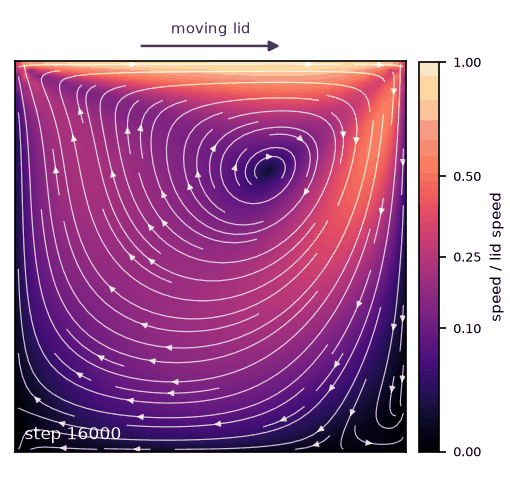
\includegraphics[height=4.4cm]{figures/cavity-movie/frame-41.png}}{figures/cavity-movie/cavity.avi}\par
    \vspace{1mm}
    {\small\textbf{Laptop}: x86 with AVX vectors\par}
    \column{0.49\textwidth}
    \centering
    \movie[loop]{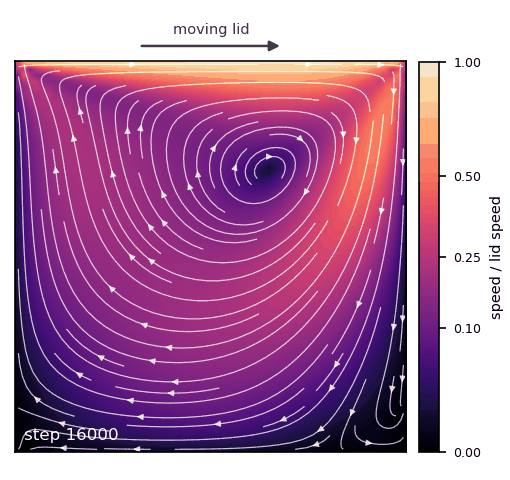
\includegraphics[height=4.4cm]{figures/cavity-movie-board/frame-41.png}}{figures/cavity-movie-board/cavity.avi}\par
    \vspace{1mm}
    {\small\textbf{K1}: RISC-V with our RVV code\par}
  \end{columns}
  \vspace{1.5mm}
  {\scriptsize\color{psgray}Middle plane of a $64^3$ box, f64, from rest to 16\,000 steps. Colour: speed; lines:
  direction of the flow. Click to play.\par}
\end{frame}
% -----------------------------------------------------------------------------
\subsection{Blocks and cores}
\begin{frame}{Running on many cores}
  \vspace{1mm}
  \centering% Slide "How waLBerla splits the work" (report r02, section "The block-structured domain" and its
% figure blockforest.tex). The benchmark uses a uniform block grid with one 64^3 block per MPI
% process and one process per core; no threads (WALBERLA_BUILD_WITH_OPENMP is OFF). The halo
% exchange copies locally between blocks of the same process and sends MPI messages otherwise;
% with one process the periodic domain makes the block its own neighbour (a local copy).
% presentation7-v3: the third panel (one RVV instruction on a row) is gone; RVV is defined only in the next section.
\begin{tikzpicture}[
    cell/.style={draw=psgray!70,line width=0.3pt},
    ttl/.style={font=\scriptsize\bfseries,anchor=south west,text=black!80,inner sep=0pt}]
  % ---- 1: the domain, one block per core ------------------------------------------
  \def\bs{0.82}
  \node[ttl] at (0,2.75) {1\enspace domain: one block per core};
  \foreach \i in {0,...,3} \foreach \j in {0,1} {
    \pgfmathtruncatemacro{\c}{\i+4*\j}
    \fill[psblue!12] (\i*\bs,0.6+\j*\bs) rectangle ++(\bs,\bs);
    \draw[psgray!80] (\i*\bs,0.6+\j*\bs) rectangle ++(\bs,\bs);
    \node[font=\tiny,text=psblue!80!black,align=center] at (\i*\bs+0.5*\bs,0.6+\j*\bs+0.5*\bs) {core\\[-2pt]\c};
  }
  \draw[black!80,line width=1pt] (2*\bs,0.6) rectangle ++(\bs,\bs);   % core 2: zoomed in panel 2
  \draw[psorange!85!black,line width=1pt,densely dashed] (3*\bs,0.6) rectangle ++(\bs,\bs); % core 3: its east neighbour
  \node[lbl,anchor=north] at (2*\bs,0.5) {8 cores: 8 blocks\\of $64^3$ cells each};
  %   zoom onto the block of panel 2
  \draw[psgray!60,dashed] (3*\bs,0.6+\bs) -- (4.3,7*0.33);
  \draw[psgray!60,dashed] (3*\bs,0.6) -- (4.3,0);

  % ---- 2: one block, its ghost layer and the halo exchange -------------------------
  %   Colours as in figures/ghost.tex: light blue = the block's cells, grey = ghost layer, orange = the neighbour's
  %   border column and the ghost column it is copied into (presentation7-v3: one picture language for all slides).
  \begin{scope}[shift={(4.3,0)}]
    \def\s{0.33}
    \node[ttl] at (0,2.75) {2\enspace one block, its ghost layer and a neighbour};
    \fill[psgray!35] (0,0) rectangle (7*\s,7*\s);
    \fill[psblue!12] (\s,\s) rectangle (6*\s,6*\s);
    \fill[psorange!55] (6*\s,\s) rectangle (7*\s,6*\s);          % its east ghost column, filled from the neighbour
    \draw[cell,step=\s] (0,0) grid (7*\s,7*\s);
    \draw[black!75,line width=0.9pt] (\s,\s) rectangle (6*\s,6*\s);
    \node[font=\scriptsize\bfseries,anchor=north] at (3.5*\s,-0.05) {block of core 2};
    %   the east neighbour, the block of core 3 (another MPI process): its first column of cells
    \begin{scope}[shift={(7*\s+0.85,0)}]
      \fill[psgray!35] (0,0) rectangle (3*\s,7*\s);
      \fill[psblue!12] (\s,\s) rectangle (3*\s,6*\s);
      \fill[psorange!55] (\s,\s) rectangle (2*\s,6*\s);
      \draw[cell,step=\s] (0,0) grid (3*\s,7*\s);
      \draw[black!75,line width=0.9pt] (3*\s,\s) -- (\s,\s) -- (\s,6*\s) -- (3*\s,6*\s);
      \node[font=\scriptsize\bfseries,anchor=north] at (1.5*\s,-0.05) {block of core 3};
    \end{scope}
    \draw[-{Stealth[length=1.8mm]},thick,psorange!85!black] (7*\s+0.85+1.5*\s,6*\s+0.02) to[out=120,in=60]
      node[above,font=\tiny,text=psorange!70!black,inner sep=1pt] {halo exchange} (6.5*\s,6*\s+0.02);
    %   legend
    \begin{scope}[shift={(0,-0.75)}]
      \draw[cell,fill=psblue!12] (0,0) rectangle ++(0.22,0.16);
      \node[lbl,anchor=west] at (0.25,0.08) {its $64^3$ cells};
      \draw[cell,fill=psgray!35] (1.9,0) rectangle ++(0.22,0.16);
      \node[lbl,anchor=west] at (2.15,0.08) {ghost layer: copies of the neighbours' border cells};
    \end{scope}
  \end{scope}
\end{tikzpicture}


  \vspace{0mm}
  \raggedright
  \begin{itemize}\small
    \item The box is cut into \term{blocks} of $64^3$ cells. Each core runs one \term{MPI} process, which owns one
          block. MPI is the library the processes use to send each other data.
    \item To update a cell at its border, a block needs cells of its neighbour. So it keeps a one-cell-thick
          \term{ghost layer} around its cells, with copies of the neighbours' border cells.
    \item After each step, the \term{halo exchange} refreshes these copies.
  \end{itemize}
  \takeaway{More cores give a larger box (\term{weak scaling}). Ideally, $N$ cores give $N$ times the MLUP/s.}
\end{frame}
% -----------------------------------------------------------------------------
\subsection{One cell and how it is stored}
% Only the last overlay (everything shown) is kept (user, 2026-11-24).
\begin{frame}<4>{The stencil: the cells needed to update one cell}
  \begin{columns}[T,onlytextwidth]
    \column{0.50\textwidth}
    \vspace{4mm}
    \centering\resizebox{\linewidth}{!}{% Slide "The stencil: the cells needed to update one cell" (new in presentation5), drawn in 3D.
% D3Q19 in lbmpy's order, the order of the generated code (direction c_i = (c_x, c_y, c_z)):
%   0 C (0,0,0)   1 N (0,1,0)   2 S (0,-1,0)  3 W (-1,0,0)  4 E (1,0,0)   5 T (0,0,1)   6 B (0,0,-1)
%   7 NW (-1,1,0) 8 NE (1,1,0)  9 SW (-1,-1,0) 10 SE (1,-1,0) 11 TN (0,1,1) 12 TS (0,-1,1) 13 TW (-1,0,1)
%   14 TE (1,0,1) 15 BN (0,1,-1) 16 BS (0,-1,-1) 17 BW (-1,0,-1) 18 BE (1,0,-1)
% Pull: the new f_i of cell x is the old f_i of the cell x - c_i. Checked against the generated StreamCollide
% (SweepgenLdcCPU_scalar_cse, build/presentation4-x86/gcc-f32, gen/SweepgenLdcCPU.cpp:44-130): f_3 is read at
% ctr_0 + 1, f_4 at ctr_0 - 1, f_1 at ctr_1 - 1, f_5 at ctr_2 - 1, f_9 at (ctr_0 + 1, ctr_1 + 1),
% f_14 at (ctr_0 - 1, ctr_2 - 1), f_17 at (ctr_0 + 1, ctr_2 + 1).
% Each dot is a cell; it is labelled with the value the update takes from it, and its arrow points the way
% that value moves (c_i), into the cell in the middle. Axes: i = +x (east), j = +y (north, into the page),
% k = +z (top); ctr_0, ctr_1, ctr_2 in the generated code.
% Overlays: 1 the 3 x 3 x 3 cells around the cell and the cell itself, 2 the 6 face neighbours (f_4 in orange:
% the example of the text), 3 the 12 edge neighbours, 4 the 8 corners, which D3Q19 does not read.
\begin{tikzpicture}[x={(1.45cm,0cm)},y={(0.78cm,0.5cm)},z={(0cm,1.45cm)}]
  \tikzset{
    lat/.style={draw=psgray!28,line width=0.35pt},
    pt/.style={circle,draw=psgray!55,fill=white,inner sep=0pt,minimum size=1.5mm},
    me/.style={circle,draw=psblue!80!black,fill=psblue!55,inner sep=0pt,minimum size=3.2mm},
    nb/.style={circle,draw=psteal!70!black,inner sep=0pt,minimum size=2.5mm},
    %   #1: the overlay on which this group appears (strong colour there, light afterwards)
    grp/.style={nb,visible on=<#1->,alt=<#1>{fill=psteal!75}{fill=psteal!30}},
    mv/.style={-{Stealth[length=1.5mm]},semithick,draw=psteal!60!black},
    fl/.style={font=\scriptsize,inner sep=0.6pt,fill=white,fill opacity=0.8,text opacity=1},
    ax/.style={-{Stealth[length=1.6mm]},thick,draw=black!75},
    axl/.style={font=\scriptsize,inner sep=1pt},
  }
  \coordinate (C) at (0,0,0);
  % ---- the 27 cells around and including the cell, with faint lattice lines (back to front)
  \foreach \a in {-1,0,1} \foreach \b in {-1,0,1} {
    \draw[lat] (-1,\a,\b) -- (1,\a,\b);
    \draw[lat] (\a,-1,\b) -- (\a,1,\b);
    \draw[lat] (\a,\b,-1) -- (\a,\b,1);
  }
  \foreach \b in {1,0,-1} \foreach \a in {-1,0,1} \foreach \c in {-1,0,1}
    \node[pt] at (\a,\b,\c) {};

  %   \nbr{overlay}{a}{b}{c}{i}: the neighbour at (a,b,c) sends f_i into the cell
  \newcommand{\nbr}[5]{%
    \coordinate (P) at (#2,#3,#4);
    \draw[mv,visible on=<#1->] ($(P)!1.6mm!(C)$) -- ($(C)!2.4mm!(P)$);
    \node[grp=#1] at (P) {};
    \node[fl,visible on=<#1->] at ($(P)!-3.4mm!(C)$) {$f_{#5}$};}
  %   back plane (y = +1) first, so the front is drawn on top
  \nbr{2}{0}{1}{0}{2}
  \nbr{3}{1}{1}{0}{9}   \nbr{3}{-1}{1}{0}{10}  \nbr{3}{0}{1}{-1}{12}  \nbr{3}{0}{1}{1}{16}
  \nbr{2}{1}{0}{0}{3}   \nbr{2}{0}{0}{-1}{5}   \nbr{2}{0}{0}{1}{6}
  \nbr{3}{1}{0}{-1}{13} \nbr{3}{-1}{0}{-1}{14} \nbr{3}{1}{0}{1}{17}   \nbr{3}{-1}{0}{1}{18}
  \nbr{2}{0}{-1}{0}{1}
  \nbr{3}{1}{-1}{0}{7}  \nbr{3}{-1}{-1}{0}{8}  \nbr{3}{0}{-1}{-1}{11} \nbr{3}{0}{-1}{1}{15}
  %   f_4 last and in orange on overlay 2: it moves east, so it comes from the west neighbour
  \coordinate (P) at (-1,0,0);
  \draw[mv,visible on=<2->,alt=<2>{draw=psorange!90!black,very thick}{}] ($(P)!1.6mm!(C)$) -- ($(C)!2.4mm!(P)$);
  \node[nb,visible on=<2->,alt=<2>{fill=psorange!70,draw=psorange!90!black}{fill=psteal!30}] at (P) {};
  \node[fl,visible on=<2->] at ($(P)!-3.4mm!(C)$) {$f_{4}$};
  % ---- the cell itself; f_0 stays
  \node[me] at (C) {};
  \node[fl,font=\scriptsize\bfseries,anchor=north west] at ([xshift=0.6mm,yshift=-0.6mm]C) {$f_0$};
  \node[font=\scriptsize,text=psblue!80!black,anchor=south east,visible on=<1>] at ([xshift=-1.5mm,yshift=1.5mm]C)
    {the cell being updated};

  % ---- 4: the 8 corners are not part of D3Q19
  \foreach \a in {-1,1} \foreach \b in {-1,1} \foreach \c in {-1,1}
    \draw[psred!80!black,semithick,visible on=<4->] ([shift={(-0.9mm,-0.9mm)}]\a,\b,\c) -- ++(1.8mm,1.8mm)
      ([shift={(-0.9mm,0.9mm)}]\a,\b,\c) -- ++(1.8mm,-1.8mm);
  \node[font=\scriptsize,text=psred!80!black,anchor=west,visible on=<4->] at ([xshift=1.5mm]1,-1,-1) {corners: not used};

  % ---- axes: the unit vectors i, j, k of x, y, z, in a corner of their own
  \begin{scope}[shift={(-3.85cm,1.15cm)}]
    \draw[ax] (0,0,0) -- (0.5,0,0) node[axl,anchor=west] {$\mathbf{i}$: $x$, east};
    \draw[ax] (0,0,0) -- (0,0.75,0) node[axl,anchor=south west] {$\mathbf{j}$: $y$, north};
    \draw[ax] (0,0,0) -- (0,0,0.5) node[axl,anchor=south] {$\mathbf{k}$: $z$, top};
  \end{scope}
\end{tikzpicture}
}
    \column{0.48\textwidth}
    \vspace{0mm}
    \begin{itemize}\small\setlength{\itemsep}{1pt}
      \item Each cell stores 19 values $f_0 \ldots f_{18}$: the fluid moving in the 19 directions $c_i$ (arrows).
      \item \textbf{Stream:} $f_i$ comes from the neighbour it moves out of, at $x - c_i$. Example: $f_4$ moves
            east, so it comes from the west neighbour.
      \item \textbf{Collide:} from these 19 values the kernel computes the cell's density $\rho$, its velocity
            $u$ and its 19 new values $f'_i$:
    \end{itemize}
    \vspace{0.5mm}
    \centering
    \colorbox{codebg}{\begin{minipage}{0.94\linewidth}\small
      \begin{tabular}{@{}r@{\hspace{2mm}}l@{}}
        {\scriptsize\color{psgray}stream} & $f^*_i = f_i(x - c_i)$\\[1pt]
        & $\rho = \sum_i f^*_i,\quad \rho\,u = \sum_i c_i\,f^*_i$\\[1pt]
        {\scriptsize\color{psgray}collide} & $f'_i(x) = f^*_i + \omega\,\bigl(f^{\mathrm{eq}}_i(\rho, u) - f^*_i\bigr)$
      \end{tabular}
    \end{minipage}}\par
    \raggedright
    {\scriptsize\color{psgray}$f^{\mathrm{eq}}_i$: the equilibrium, a fixed formula in $\rho$ and $u$. $\omega$: a
    constant. This is the \term{SRT} model (single relaxation time).\par}
  \end{columns}
  \takeaway{The kernel reads 19 values $f_i$ from the \term{stencil} (the cell, 6 face and 12 edge neighbours) and
    writes the cell's 19 new values $f'_i$.}
\end{frame}
% -----------------------------------------------------------------------------
%  figures/fzyx.tex and figures/ghost.tex have the sources (waLBerla's Field.hpp, the strides of our arrays).
\begin{frame}{How the 19 values are stored in memory}
  \vspace{0mm}
  \begin{columns}[T,onlytextwidth]
    \column{0.53\textwidth}
    {\small\bfseries Layout \term{fzyx}: each value has its own array\par}
    \vspace{1mm}
    \begin{tikzpicture}
      \node[codebox,font=\ttfamily\scriptsize,anchor=north west,inner sep=3pt] {%
        f\ =\ np.empty((19,\ 66,\ 66,\ 68),\ np.float32)\ \textcolor{psgray}{\#\ A:\ $f_i$}\\
        g\ =\ np.empty\_like(f)\ \ \ \ \ \ \ \ \ \ \ \ \ \ \ \ \ \ \ \ \ \ \ \textcolor{psgray}{\#\ B:\ $f'_i$}\\
        \textcolor{psorange!85!black}{\textbf{f[i,\ z,\ y,\ x]}}\ \ \ \ \ \ \ \ \ \ \textcolor{psgray}{\#\ the\ value\ $f_i$\ of\ cell\ (x,\ y,\ z)}};
    \end{tikzpicture}\par
    {\tiny\color{psgray}66 = 64 cells + 2 ghost cells (at $-1$ and 64); 68 = 66 + 2 values of padding (f32 only).\par}
    \vspace{0.5mm}
    % presentation7-v3: the field is drawn twice, A (f, the values f_i) and B (g, the new values f'_i), as the two
% buffers of the pull pattern (lbm_bulk.py: pdfs and pdfs_tmp, swapped after every sweep).
% Slide "How the 19 values are stored in memory", left picture (presentation7-v2, replaces field-layout.tex after
% the user's review): the field f in waLBerla's layout fzyx, zoomed in four levels.
% As an ndarray (C order, last index fastest): float f[19][66][66][68], value f_i of cell (x, y, z) = f[i][z][y][x]
% (f32; f64: double f[19][66][66][66]). The name fzyx lists the axes from slowest to fastest, as the declaration.
% Source: submodules/walberla/include/walberla/v8/memory/Field.hpp:215-252: ONE buffer per field, allocated shape
% (64 + 2 ghost) per axis and F_SIZE = 19, linearization order x, y, z, f (x fastest, f slowest), offsets = the
% ghost layer (so x = 0 is the first cell of the block, the ghost cell is x = -1), and for fzyx each x line padded
% to the alignment (BufferSystem.hpp:441-452; 16 B: 66 f32 = 264 B become 68 f32 = 272 B; 66 f64 = 528 B need no
% padding). Strides in f32 values: y 68, z 68 * 66 = 4488, f 4488 * 66 = 296208 (17 952 B and 1 184 832 B);
% f64: 66, 4356, 287496. The index is the one of the generated kernels (_data_f[x + y * _stride_f_1 + z *
% _stride_f_2 + i * _stride_f_3]).
\begin{tikzpicture}[x=1cm,y=1cm]
  \tikzset{sg/.style={draw=psgray!70,line width=0.3pt,minimum height=4.2mm,inner sep=0pt,font=\tiny,anchor=west},
           hi/.style={fill=psblue!25,draw=psblue!80!black},
           gh/.style={fill=psgray!35},
           pd/.style={fill=white,densely dashed},
           zl/.style={densely dashed,psgray!70},
           br/.style={decorate,decoration={brace,amplitude=2.5pt,mirror},psgray!90!black},
           bl/.style={font=\tiny,text=psgray!90!black,inner sep=1pt},
           lv/.style={font=\scriptsize\bfseries,anchor=east,inner sep=1pt}}
  \def\W{6.6}
  % ---- level 1: the whole field, 19 arrays one after the other ------------------------------
  \node[lv] at (-0.05,0) {A};
  \foreach \i in {0,...,18} {
    \pgfmathsetmacro\xx{\i*\W/19}
    \ifnum\i=0 \node[sg,hi,minimum width=\W/19 cm] (a\i) at (\xx,0) {$f_0$};
    \else\ifnum\i<3 \node[sg,minimum width=\W/19 cm] (a\i) at (\xx,0) {$f_{\i}$};
    \else\ifnum\i=18 \node[sg,minimum width=\W/19 cm] (a\i) at (\xx,0) {\tiny$f_{18}$};
    \else \node[sg,minimum width=\W/19 cm] (a\i) at (\xx,0) {};\fi\fi\fi
  }
  \node[bl,anchor=south] at (\W/2,0.22) {A: the 19 arrays $f_0 \ldots f_{18}$, one after the other. B: the same for $f'_0 \ldots f'_{18}$.};
  % ---- level 2: one array = 66 planes --------------------------------------------------------
  \def\y{-1.3}
  \node[lv] at (-0.05,\y) {$f_0$};
  \foreach \k/\t/\st in {0/ghost/gh, 1/{$z{=}0$}/hi, 2/{$z{=}1$}/, 3/{$\cdots$}/, 4/{$z{=}63$}/, 5/ghost/gh}
    \node[sg,\st,minimum width=1.1cm] (b\k) at (\k*1.1,\y) {\t};
  \draw[zl] (a0.south west) -- (0,-0.72) -- (b0.north west);   % behind the B row, drawn next
  \draw[zl] (a0.south east) -- (\W/19,-0.72) -- (b5.north east);
  % ---- level 1b: the second field B, same shape, for the new values f'_i (presentation7-v3) ----------
  \node[lv] at (-0.05,-0.5) {B};
  \foreach \i in {0,...,18} {
    \pgfmathsetmacro\xx{\i*\W/19}
    \ifnum\i<3 \node[sg,fill=psorange!12,minimum width=\W/19 cm] at (\xx,-0.5) {$f'_{\i}$};
    \else\ifnum\i=18 \node[sg,fill=psorange!12,minimum width=\W/19 cm] at (\xx,-0.5) {\tiny$f'_{18}$};
    \else \node[sg,fill=psorange!12,minimum width=\W/19 cm] at (\xx,-0.5) {};\fi\fi
  }
  \draw[br] (b1.south west) -- (b1.south east) node[midway,below=2pt,bl] {one plane: 18\,KB};
  \node[bl,anchor=north east] at (\W,\y-0.22) {one array: 66 planes, 1.2\,MB};
  % ---- level 3: one plane = 66 rows ------------------------------------------------------------
  \def\y{-2.15}
  \node[lv] at (-0.05,\y) {plane};
  \foreach \k/\t/\st in {0/ghost/gh, 1/{$y{=}0$}/hi, 2/{$y{=}1$}/, 3/{$\cdots$}/, 4/{$y{=}63$}/, 5/ghost/gh}
    \node[sg,\st,minimum width=1.1cm] (c\k) at (\k*1.1,\y) {\t};
  \draw[zl] (b1.south west) -- (c0.north west);
  \draw[zl] (b1.south east) -- (c5.north east);
  \draw[br] (c1.south west) -- (c1.south east) node[midway,below=2pt,bl] {one row: 272\,B};
  % ---- level 4: one row = 1 ghost + 64 cells + 1 ghost + 2 padding ------------------------------
  \def\y{-3.0}
  \node[lv] at (-0.05,\y) {row};
  \def\cw{0.42}
  \foreach \k/\t/\st in {0/{}/gh, 1/{0}/hi, 2/{1}/hi, 3/{2}/hi, 4/{3}/hi, 5/{}/, 6/{$\cdots$}/, 7/{}/, 8/{62}/hi,
                         9/{63}/hi, 10/{}/gh, 11/{}/pd, 12/{}/pd}
    \node[sg,\st,minimum width=\cw cm] (d\k) at ({\k*\cw},\y) {\t};
  \draw[zl] (c1.south west) -- (d0.north west);
  \draw[zl] (c1.south east) -- (d12.north east);
  \draw[br] (d1.south west) -- (d9.south east) node[midway,below=2pt,bl] {the 64 cells $x = 0 \ldots 63$, a ghost cell at each end};
  \node[bl,anchor=west,align=left] at ([xshift=1mm]d12.east) {2 values of\\padding};
\end{tikzpicture}%

    \column{0.44\textwidth}
    {\small\bfseries The \term{ghost layer} and the \term{halo exchange}\par}
    \vspace{2mm}
    \centering\resizebox{\linewidth}{!}{% Slide "How the 19 values are stored in memory", right picture (presentation7-v2, after the user's review: the
% ghost layer was vague). A cut through two neighbouring blocks (x-y plane), 64 x 64 cells drawn as 5 x 5.
% Facts: one ghost layer on every face (Field.hpp:215-226: allocShape = shape + 2 * numGhostLayers, 64^3 -> 66^3
% cells per array; 66^3 / 64^3 = 1.097). The kernel reads its neighbours' values from the ghost layer (pull
% streaming: the value moving east into a border cell comes from x - 1, which for x = 0 is the ghost cell) and
% writes only the 64^3 inner cells. After each step the halo exchange copies every block's border cells into the
% neighbours' ghost layers (MPI between processes; figures/parallel.tex, time-step.tex). The picture names the two
% copies "halo exchange" and points at the grey ring as the "ghost layer".
\begin{tikzpicture}[x=1cm,y=1cm]
  \def\c{0.33}
  \tikzset{cl/.style={draw=psgray!60,line width=0.3pt},
           inner cell/.style={cl,fill=psblue!12}, ghost cell/.style={cl,fill=psgray!35},
           sa/.style={cl,fill=psteal!55}, sb/.style={cl,fill=psorange!55},
           bl/.style={font=\tiny,text=psgray!90!black,inner sep=1pt,align=center},
           cp/.style={-{Stealth[length=1.8mm]},thick}}
  %   \blk{x offset}{name}: a block of 5 x 5 inner cells with its ghost ring (7 x 7)
  \def\blk#1#2{%
    \foreach \i in {0,...,6} \foreach \j in {0,...,6} {
      \ifnum\i=0 \def\st{ghost cell}\else\ifnum\i=6 \def\st{ghost cell}\else\ifnum\j=0 \def\st{ghost cell}\else\ifnum\j=6 \def\st{ghost cell}\else
        \def\st{inner cell}\fi\fi\fi\fi
      \draw[\st] (#1+\i*\c,\j*\c) rectangle ++(\c,\c);}
    \draw[black!75,line width=0.9pt] (#1+\c,\c) rectangle ++(5*\c,5*\c);
    \node[font=\scriptsize\bfseries,anchor=north] at (#1+3.5*\c,-0.05) {#2};}
  \blk{0}{core 2}
  \blk{3.1}{core 3}
  %   the border columns that are copied, and where they go
  \foreach \j in {1,...,5} {
    \draw[sa] (5*\c,\j*\c) rectangle ++(\c,\c);           % A's last inner column
    \draw[sa] (3.1,\j*\c) rectangle ++(\c,\c);             % -> B's ghost column
    \draw[sb] (3.1+\c,\j*\c) rectangle ++(\c,\c);         % B's first inner column
    \draw[sb] (6*\c,\j*\c) rectangle ++(\c,\c);           % -> A's ghost column
  }
  %   the blocks' bold outlines again, on top of the coloured columns (otherwise those hide them)
  \draw[black!75,line width=0.9pt] (\c,\c) rectangle ++(5*\c,5*\c);
  \draw[black!75,line width=0.9pt] (3.1+\c,\c) rectangle ++(5*\c,5*\c);
  \draw[cp,psteal!70!black] (5.5*\c,6*\c+0.02) to[out=60,in=120] node[pos=0.5,above,bl,text=psteal!50!black]
    (top) {core 2's border cells $\rightarrow$ core 3's ghost layer} (3.1+0.5*\c,6*\c+0.02);
  %   the two copies together are the halo exchange (user's review 2026-11-25: name it in the picture)
  \node[font=\scriptsize\bfseries,text=black!80,anchor=south,inner sep=1pt] at (top.north)
    {halo exchange, after every step:};
  %   point at the grey ring itself
  \node[bl,text=black!70,anchor=north] (gl) at (0.1,-0.32) {ghost layer};
  \draw[-{Stealth[length=1.4mm]},black!60,line width=0.5pt] (gl.north) -- (0.5*\c,1.5*\c);
  %   "halo" is another name for the same ring (the halo exchange refills it)
  \node[bl,text=black!70,anchor=west,align=left] (hl) at (3.1+7*\c+0.25,3.5*\c) {halo =\\ghost\\layer};
  \draw[-{Stealth[length=1.4mm]},black!60,line width=0.5pt] (hl.west) -- (3.1+6.5*\c,3.5*\c);
  \draw[cp,psorange!85!black] (3.1+1.5*\c,-0.02) to[out=-120,in=-60] node[pos=0.5,below,bl,text=psorange!70!black]
    {core 3's border cells $\rightarrow$ core 2's ghost layer} (6.5*\c,-0.02);
  %   legend
  \begin{scope}[shift={(0,-1.1)}]
    \draw[inner cell] (0,0) rectangle ++(0.25,0.18); \node[bl,anchor=west] at (0.3,0.09) {the block's 64$^3$ cells};
    \draw[ghost cell] (2.35,0) rectangle ++(0.25,0.18); \node[bl,anchor=west] at (2.65,0.09) {ghost layer: one cell thick};
  \end{scope}
\end{tikzpicture}%
}

    \vspace{1mm}
    \raggedright
    {\scriptsize A $64^3$ block is stored as $66^3$ cells, in A and in B. The kernel reads A (ghost layer
    included) and writes the inner cells of B. The halo exchange then fills B's ghost layer, and A and B swap.\par}
  \end{columns}
  \takeaway{fzyx means \code{f[i, z, y, x]}: $x$ is the fastest index. The 19 values of one cell are 1.2\,MB apart.}
\end{frame}
% -----------------------------------------------------------------------------
\subsection{One time step}
%  figures/time-step.tex has the sources (order of the time loop, the three timers of the app).
\begin{frame}{What one time step does}
  \vspace{1.5mm}
  \centering% Slide "What one time step does" (new in presentation7-v2, so that "wall pass" is defined before the time-share
% plots use it). The order in the benchmark's time loop (submodules/walberla/apps/benchmarks/SweepgenLdcCPU/
% SweepgenLdcCPU.cpp:33-35 and 210-256): StreamCollide (the kernel), then the halo exchange (streamPullSync, or
% aaPullSync / aaPushSync), then NoSlip and UBB on the wall links (the wall pass). The app times the three parts
% separately: t_bulk, t_comm, t_bc (line 361), which are the three colours of the time-share plots.
% Bottom: the wall rule (bounce-back) in 2D. NoSlip: a value that would stream into a fixed wall comes back in the
% opposite direction. UBB (the lid): the same, plus a small change that carries the lid's speed into the fluid.
% The wall pass is generated for Target.GenericCPU in every variant (SweepgenLdcCPU.py:28-29, 135-141).
% Segment widths are only a sketch; the measured shares are on the "where the time goes" slides.
\begin{tikzpicture}[x=1cm,y=1cm]
  \tikzset{seg/.style={draw=white,line width=0.8pt,minimum height=7mm,inner sep=2pt,font=\scriptsize,
             align=center,anchor=west},
           dsc/.style={font=\scriptsize,align=left,anchor=north west,inner sep=0pt,text width=#1},
           cellb/.style={draw=psgray!55,line width=0.3pt,fill=psteal!8}}
  % ---- one time step: three parts, one after the other -------------------------------
  \node[font=\scriptsize\bfseries,anchor=south west,inner sep=0pt] at (0,0.45) {one time step};
  \node[seg,fill=ckernel,text=white,minimum width=7.6cm] (k) at (0,0) {\textbf{1.\ kernel}};
  \node[seg,fill=ccomm,minimum width=2.6cm] (h) at (k.east) {\textbf{2.\ halo exchange}};
  \node[seg,fill=cwall,minimum width=2.6cm] (w) at (h.east) {\textbf{3.\ wall pass}};
  \draw[arr] (0,-0.5) -- (12.8,-0.5) node[pos=0.5,below,lbl] {time; then A and B swap, and the next step starts};
  \node[dsc=7.3cm] at (0.05,-0.95) {For every cell: read its 19 values $f_i$ from A (stream), compute the 19 new
    values $f'_i$ (collide) and write them into B. This part is generated code.};
  \node[dsc=2.5cm] at (7.7,-0.95) {Each block copies its border cells of B into its neighbours' ghost layers (MPI).};
  \node[dsc=2.5cm] at (10.3,-0.95) {The cells next to a wall are corrected.};

  % ---- the wall rule: bounce-back ------------------------------------------------------
  \begin{scope}[shift={(0.6,-4.25)}]
    \def\s{0.5}
    %   fixed wall below, the lid above, fluid cells between
    \fill[pattern=north east lines,pattern color=psgray!80] (0,-0.13) rectangle (6*\s,0);
    \fill[psorange!55] (0,3*\s) rectangle (6*\s,3*\s+0.13);
    \foreach \i in {0,...,5} \foreach \j in {0,1,2} \draw[cellb] (\i*\s,\j*\s) rectangle ++(\s,\s);
    \draw[arr,psorange!85!black,very thick] (1.0,3*\s+0.3) -- ++(1.0,0)
      node[right,font=\tiny,text=psorange!85!black] {moving lid};
    \node[font=\tiny,text=psgray!90!black,anchor=north] at (3*\s,-0.15) {fixed wall};
    %   a value heading into the fixed wall comes back the other way
    \draw[-{Stealth[length=1.6mm]},thick,psblue!85!black] (1.5*\s,0.5*\s+0.25) -- (1.5*\s+0.22,0.03);
    \draw[-{Stealth[length=1.6mm]},thick,psred!85!black] (1.5*\s+0.18,0.06) -- (1.5*\s-0.06,0.5*\s+0.27);
    %   and one heading into the lid
    \draw[-{Stealth[length=1.6mm]},thick,psblue!85!black] (4.5*\s,2.5*\s-0.25) -- (4.5*\s+0.22,3*\s-0.03);
    \draw[-{Stealth[length=1.6mm]},thick,psred!85!black] (4.5*\s+0.18,3*\s-0.06) -- (4.5*\s-0.12,2.5*\s-0.2);
  \end{scope}
  \node[dsc=8.7cm] at (4.3,-2.6) {%
    \textbf{The wall rule (bounce-back).} A value that would flow into a wall
    (\textcolor{psblue!85!black}{blue}) comes back in the opposite direction
    (\textcolor{psred!85!black}{red}). At the moving lid it also picks up some of the lid's speed: this is what
    drives the flow.\\[3pt]
    The wall pass applies this rule to the cells next to the walls only. Its code is plain C++, never vector
    code, so it does not get faster when the kernel does.};
\end{tikzpicture}%

  \takeaway{Each time step has three parts: the \term{kernel}, the \term{halo exchange} and the \term{wall pass}.
    Only the kernel is generated, and our work makes it faster.}
\end{frame}
% -----------------------------------------------------------------------------
\subsection{Cache lines and data streams}
%  figures/stream-why.tex has the sources (cache line sizes, the stream limit of the K1, the 42 arrays).
\begin{frame}{What a stream is, and why it matters}
  \vspace{2mm}
  \centering% Slide "What a stream is, and why it matters" (presentation7-v2; replaces cache-line.tex and stream-count.tex after
% the user's review: one picture instead of 5 overlays).
% Cache line 64 B: K1 read on the board (sysfs coherency_line_size, device tree); SG2044 read on monte3 (sysfs
% coherency_line_size = 64 for index0-3, 2026-11-25). 64 B = 16 f32 = 8 f64.
% Left: one array read along x; lines already used, the line in use, two lines the hardware prefetcher has
% requested after seeing the regular pattern, lines not touched yet.
% Right: the prefetcher follows a limited number of streams: on the K1 about 20 (Part 1, figures/streams.tex: up
% to 19 read streams the lines arrive in time, from about 21 on every vector load waits, about 360 cycles).
% Our loop: 19 read + 19 written + 4 outputs = 42 arrays = 42 streams (AB pattern; stream-def.tex).
\begin{tikzpicture}[x=1cm,y=1cm]
  \tikzset{ln/.style={draw=black!75,line width=0.8pt},
           sub/.style={draw=psgray!40,line width=0.2pt},
           done/.style={fill=psgray!30}, now/.style={fill=psteal!65}, nxt/.style={fill=psteal!20},
           pfb/.style={box,info,font=\scriptsize,align=center,inner sep=2pt,minimum height=5mm},
           ttl/.style={font=\small\bfseries,anchor=west,inner sep=0pt},
           tx/.style={font=\scriptsize,align=left,anchor=north west,inner sep=0pt},
           bl/.style={font=\tiny,text=psgray!90!black,inner sep=1pt,align=center}}
  \path (0,0.2) rectangle (14.2,4.45);
  % ================= 1: what a stream is ===================================================
  \node[ttl] at (0,4.3) {1.\ A stream};
  \begin{scope}[shift={(2.2,4.22)}]
    \fill[done] (0,0) rectangle ++(0.28,0.16); \node[bl,anchor=west] at (0.32,0.08) {used};
    \fill[now] (1.05,0) rectangle ++(0.28,0.16); \node[bl,anchor=west] at (1.37,0.08) {in use};
    \fill[nxt] (2.2,0) rectangle ++(0.28,0.16); \draw[psgray!40] (2.2,0) rectangle ++(0.28,0.16);
    \node[bl,anchor=west] at (2.52,0.08) {loaded early};
  \end{scope}
  \def\sx{1.05}\def\lw{0.66}\def\sy{2.3}\def\sh{0.48}
  \foreach \k/\st in {0/done,1/done,2/done,3/now,4/nxt,5/nxt,6/,7/} {
    \ifx\st\empty\else\fill[\st] (\sx+\k*\lw,\sy) rectangle ++(\lw,\sh);\fi
    \foreach \j in {1,...,15} \draw[sub] (\sx+\k*\lw+\j*\lw/16,\sy) -- ++(0,\sh);
    \draw[ln] (\sx+\k*\lw,\sy) rectangle ++(\lw,\sh);
  }
  \node[font=\scriptsize,anchor=east] at (\sx-0.06,\sy+\sh/2) {array $f_0$};
  \draw[arr] (\sx,\sy-0.18) -- (\sx+8*\lw,\sy-0.18) node[pos=0.33,below,bl] {addresses grow: the loop walks along $x$};
  \draw[decorate,decoration={brace,amplitude=2.5pt,mirror},psgray!90!black] (\sx+7*\lw,\sy-0.5) -- (\sx+8*\lw,\sy-0.5);
  \node[bl,anchor=north east] at (\sx+8*\lw,\sy-0.62) {one cache line: 64 B = 16 f32 or 8 f64};
  %   the loop and the prefetcher
  \node[font=\scriptsize,text=psteal!40!black,anchor=south,align=center] (lp) at (\sx+1.3*\lw,\sy+0.9) {the loop\\reads here};
  \draw[-{Stealth[length=1.8mm]},thick,psteal!60!black] (lp.south) -- (\sx+3.5*\lw,\sy+\sh+0.04);
  \node[pfb,anchor=south,text width=3.3cm] (pf) at (\sx+5.0*\lw,\sy+0.9)
    {\textbf{hardware prefetcher}: sees line after line, loads the next two early};
  \draw[-{Stealth[length=1.8mm]},thick,psblue!70!black] (pf.south) -- (\sx+4.5*\lw,\sy+\sh+0.04);
  \draw[-{Stealth[length=1.8mm]},thick,psblue!70!black] (pf.south) -- (\sx+5.5*\lw,\sy+\sh+0.04);
  \node[tx,text width=6.5cm] at (0,1.3) {A \term{stream} is one array that the loop walks through, one cache line
    after the other. The prefetcher sees this pattern and loads the next lines \textbf{before} the loop needs
    them. So the loads do not wait for memory.};

  % ================= 2: why the number of streams matters ==============================================
  \draw[psgray!40] (6.85,4.45) -- (6.85,0.2);
  \node[ttl] at (7.1,4.3) {2.\ Why the number matters};
  \node[font=\scriptsize,anchor=west,inner sep=0pt] at (7.1,3.92) {Our loop walks through \textbf{42 arrays}: 42 streams.};
  \def\xa{7.85}
  \foreach \r/\t/\ok in {0/{$f_0$}/1, 1/{$f_1$}/1, 2/{$f_2$}/1, 4/{$f_{18}$}/1, 5/{$f'_0$}/1, 7/{$f'_{18}$}/0,
                         8/{$\rho$}/0, 10/{$u_z$}/0} {
    \pgfmathsetmacro\yy{3.38-\r*0.3}
    \foreach \k in {0,...,7} \draw[draw=psgray!60,line width=0.2pt] (\xa+\k*0.18,\yy) rectangle ++(0.18,0.22);
    \fill[psteal!65] (\xa+3*0.18,\yy) rectangle ++(0.18,0.22);
    \ifnum\ok=1 \fill[psteal!20] (\xa+4*0.18,\yy) rectangle ++(0.36,0.22);\fi
    \draw[black!70,line width=0.5pt] (\xa,\yy) rectangle ++(1.44,0.22);
    \node[font=\tiny,anchor=east] at (\xa-0.05,\yy+0.11) {\t};
    \ifnum\ok=1
      \coordinate (s\r) at (\xa+1.48,\yy+0.11);
    \else
      \node[font=\small\bfseries,text=psred!85!black] at (\xa+1.7,\yy+0.11) {$\times$};
    \fi
  }
  \foreach \r in {3,6,9} \node[font=\tiny,text=psgray] at (\xa+0.72,{3.38-\r*0.3+0.13}) {$\vdots$};
  \node[pfb,anchor=north west,text width=3.3cm] (tab) at (10.75,3.5)
    {\textbf{hardware prefetcher}: follows only a limited number of streams, about 20 on the K1};
  \foreach \r in {0,1,2,4,5} \draw[psblue!70!black,semithick] (s\r) -- ([yshift={(2-\r)*0.6mm}]tab.west);
  \node[tx,text width=3.4cm,text=psred!70!black] at (10.75,2.15)
    {$\times$ The other streams get no help. Each of their cache lines comes from memory while the core
     waits: about 360 cycles on the K1.};
\end{tikzpicture}%


  \vspace{1mm}
  \raggedright
  {\scriptsize\color{psgray}Cache lines are 64 bytes on both machines. The limit of about 20 streams is measured on
  the K1, in the next section.\par}
  \takeaway{A stream is one array walked through line by line. The prefetcher helps every stream it follows, but
    it can follow only about 20, and our loop has 42.}
\end{frame}
% -----------------------------------------------------------------------------
\begin{frame}{Our loop walks through 42 arrays at once}
  \begin{columns}[T,onlytextwidth]
    \column{0.52\textwidth}
    \vspace{1mm}
    \centering% Slide "What a data stream is": the memory one step of the inner loop touches (AB pattern, the
% generated StreamCollide kernel). Each of the 19 values of a cell has its own array (waLBerla's
% fzyx layout); pull streaming reads value i at the neighbour x - c_i (still consecutive addresses
% along x), the AB pattern writes a second set of 19 arrays, and the kernel writes rho and u
% (4 arrays): 19 + 19 + 4 = 42 sequences of consecutive addresses, all advancing together.
% Evidence: the generated StreamCollide of SweepgenLdcCPU_explicit_cse_pf (GCC f32, board) has
% exactly 19 prefetch_read and 23 prefetch_write calls in its loop, one per array it walks through.
% presentation7-v2: no overlays any more (the single-array animation moved to figures/cache-line.tex). Every box
% is one cache line of 64 bytes; all 42 arrays are at the same place of the loop (line 5).
\begin{tikzpicture}[x=1cm,y=1cm]
  \tikzset{cl/.style={draw=psgray!70,fill=white,line width=0.3pt},
           clnow/.style={draw=psteal!80!black,fill=psteal!65,line width=0.3pt},
           clnext/.style={draw=psteal!60,fill=psteal!18,line width=0.3pt},
           cldone/.style={draw=psgray!70,fill=psgray!28,line width=0.3pt},
           arrlbl/.style={font=\scriptsize,anchor=east,inner sep=1pt}}
  %   \strip{y}{label}: one array as 10 cache lines; the loop is in line 5, the two after it are on their way
  \newcommand{\strip}[2]{%
    \foreach \k in {0,...,9} {
      \ifnum\k<5 \def\st{cldone}\else\ifnum\k=5 \def\st{clnow}\else
        \ifnum\k<8 \def\st{clnext}\else \def\st{cl}\fi\fi\fi
      \draw[\st] (\k*0.4,#1) rectangle ++(0.4,0.22);
    }
    \node[arrlbl] at (-0.05,#1+0.11) {#2};}
  \newcommand{\vdotsat}[1]{\node[font=\scriptsize,text=psgray] at (2.2,#1) {$\vdots$};}
  \newcommand{\grp}[4]{% y bottom, y top, count, what
    \draw[decorate,decoration={brace,amplitude=3pt},psgray!90!black] (4.15,#2) -- (4.15,#1)
      node[midway,right=3pt,font=\scriptsize,align=left] {\textbf{#3} #4};}

  \strip{3.5}{$f_0$} \strip{3.23}{$f_1$} \vdotsat{2.98} \strip{2.62}{$f_{18}$}
  \grp{2.62}{3.72}{19}{read\\from A}
  \strip{2.12}{$f'_0$} \strip{1.85}{$f'_1$} \vdotsat{1.6} \strip{1.24}{$f'_{18}$}
  \grp{1.24}{2.34}{19}{written\\into B}
  \strip{0.74}{$\rho$} \strip{0.47}{$u_x$} \vdotsat{0.22} \strip{-0.14}{$u_z$}
  \grp{-0.14}{0.96}{4}{outputs}
  \node[font=\tiny,text=psteal!50!black,anchor=south,inner sep=1pt] at (5*0.4+0.2,3.74) {$\downarrow$ loop};

  \draw[arr] (0,-0.42) -- (4.0,-0.42) node[midway,below,lbl] {the loop goes along $x$: addresses grow};
  \node[draw=psteal!80!black,fill=psteal!8,rounded corners=2pt,font=\small\bfseries,anchor=west]
    at (4.3,-0.45) {= 42 streams};
  %   legend
  \node[lbl,anchor=west] at (-0.05,4.55) {each box is one cache line of 64 bytes};
  \draw[clnow] (0,4.1) rectangle ++(0.3,0.18);
  \node[lbl,anchor=west] at (0.35,4.19) {in use};
  \draw[clnext] (1.35,4.1) rectangle ++(0.3,0.18);
  \node[lbl,anchor=west] at (1.7,4.19) {loading early};
  \draw[cldone] (3.65,4.1) rectangle ++(0.3,0.18);
  \node[lbl,anchor=west] at (4.0,4.19) {already used};
\end{tikzpicture}

    \column{0.46\textwidth}
    \vspace{1mm}
    {\small What the rows are:\par}
    \vspace{1mm}
    \begin{itemize}\small
      \item $f_0$ to $f_{18}$: the 19 values of each cell \emph{before} the time step. The loop reads them from
            the 19 arrays of A.
      \item $f'_0$ to $f'_{18}$: the 19 new values \emph{after} the step. The loop writes them into the 19
            arrays of B.
      \item $\rho$: the \term{density} of the fluid in each cell. $u_x$, $u_y$, $u_z$: the three parts of its
            \term{velocity}. The loop writes these 4 outputs too.
    \end{itemize}
    \vspace{1mm}
    {\small All 42 arrays advance together, one cache line after the other. The hardware prefetcher can follow
    only a limited number of streams at once.\par}
  \end{columns}
  \takeaway{19 reads + 19 writes + 4 outputs = 42 streams at once.}
\end{frame}
% -----------------------------------------------------------------------------
\subsection{Two ways to use fewer streams: AA and the split loop}
\begin{frame}{Fewer streams, way 1: update in place (the AA pattern)}
  \vspace{1mm}
  \begin{columns}[T,onlytextwidth]
    \column{0.4\textwidth}
    {\small\bfseries The usual way (AB): read A, write B\par}
    \vspace{3mm}
    \centering% The usual "AB" scheme: two sets of 19 arrays, A (f, the values f_i) and B (g, the new values f'_i), drawn as the
% two field rows of the slide "How the 19 values are stored in memory" (figures/fzyx.tex). Each step reads one set
% and writes the other; then they swap roles (lbm_bulk.py: swap_fields(pdfs, pdfs_tmp) after every sweep).
% presentation7-v3: A and B look the same as where they are introduced.
\begin{tikzpicture}[x=1cm,y=1cm]
  \tikzset{ca/.style={draw=psgray!70,line width=0.3pt,minimum height=4.2mm,minimum width=2.7mm,inner sep=0pt,
             font=\tiny,anchor=west},
           cb/.style={ca,fill=psorange!12},
           st/.style={-{Stealth[length=1.8mm]},thick}}
  \def\w{0.27}
  %   \fieldrow{y}{style}{prime}: 19 arrays, the first three and the last labelled
  \newcommand{\fieldrow}[3]{%
    \foreach \i in {0,...,18} {
      \ifnum\i<2 \node[#2] at (\i*\w,#1) {$f#3_{\i}$};
      \else\ifnum\i=18 \node[#2] at (\i*\w,#1) {\tiny$f#3_{18}$};
      \else \node[#2] at (\i*\w,#1) {};\fi\fi}}
  \fieldrow{0}{ca}{}
  \fieldrow{-2.0}{cb}{'}
  \node[font=\small\bfseries,anchor=east] at (-0.1,0) {A};
  \node[font=\small\bfseries,anchor=east] at (-0.1,-2.0) {B};
  \draw[st,psblue!85!black] (1.3,-0.3) -- node[left,font=\scriptsize,align=right,text=black] {step 1:\\read A,\\write B} (1.3,-1.7);
  \draw[st,psorange!90!black] (3.9,-1.7) -- node[right,font=\scriptsize,align=left,text=black] {step 2:\\read B,\\write A} (3.9,-0.3);
  \node[lbl,anchor=north,align=center] at (19*\w/2,-2.35) {two full copies of the 19 arrays;\\they swap roles after every step};
\end{tikzpicture}


    \vspace{1mm}
    {\small\textbf{42 streams}, 260 bytes per cell\par}
    \column{0.56\textwidth}
    {\small\bfseries In place (AA): only A, two kinds of step\par}
    \vspace{1mm}
    \centering% Slide "Fewer streams, way 1: update in place (the AA pattern)": the AA pattern for one pair of directions,
% seen from cell x (as in lbmpy's AA accessors). Two of a cell's 19 slots are drawn: the slot of f_3 (the value
% moving west, D3Q19 in lbmpy's order: c_3 = (-1, 0, 0)) and the slot of f_4 (moving east, c_4 = (+1, 0, 0)).
% Even step: read both slots of x, collide, write each new value into the slot of the OPPOSITE direction of the
% same cell (so the two values swap slots and nothing moves yet). Odd step: read from the neighbours' slots (f_3
% of x-1, f_4 of x+1, where the even step left the values) and write the new values back into the same slots,
% which completes the move of both steps. Every step reads and writes the same addresses: one set of arrays.
% presentation7-v2 (user's review): the slots were labelled W and E without a definition; now f_3 and f_4 with
% arrows, and a legend that says what they are.
\begin{tikzpicture}[
    slot/.style={draw=psgray!80,fill=codebg,minimum width=6.4mm,minimum height=4.6mm,inner sep=0pt,font=\tiny},
    coll/.style={circle,draw=psgray!90,fill=white,inner sep=1pt,font=\tiny},
    rd/.style={-{Stealth[length=1.4mm]},semithick,draw=psblue!85!black,dashed},
    wr/.style={-{Stealth[length=1.4mm]},semithick,draw=psorange!90!black}]
  \foreach \p/\py/\ttl in {e/0/{even step: the new values stay in cell $x$, in swapped slots},
                           o/-1.95/{odd step: read the neighbours' slots, write back there}} {
    \foreach \c/\lab in {0/$x{-}1$, 1/$x$, 2/$x{+}1$} {
      \node[slot] (\p W\c) at (\c*1.66+0.3,\py) {$f_3\,\leftarrow$};
      \node[slot] (\p E\c) at (\c*1.66+0.94,\py) {$f_4\,\rightarrow$};
      \node[font=\tiny,text=psgray] at (\c*1.66+0.62,\py-0.38) {cell \lab};
    }
    \node[coll] (\p col) at (2.28,\py+0.85) {collide};
    \node[font=\scriptsize\bfseries,anchor=west] at (-0.05,\py+1.3) {\ttl};
  }
  %   even step: read both slots of x, write each new value into the other slot
  \draw[rd] (eE1.north) to[bend right=10] (ecol);
  \draw[rd] (eW1.north) to[bend left=10] (ecol);
  \draw[wr] (ecol.west) to[bend right=45] (eW1.north west);
  \draw[wr] (ecol.east) to[bend left=45] (eE1.north east);
  %   odd step: the value coming from x-1 (moving east) sits in the f_3 slot of x-1, where the even step put it;
  %   the one coming from x+1 (moving west) in the f_4 slot of x+1. The new values go back into the same two slots.
  \draw[rd] (oW0.north) to[bend left=10] (ocol);
  \draw[rd] (oE2.north) to[bend right=10] (ocol);
  \draw[wr] (ocol.east) to[bend left=20] (oE2.north west);
  \draw[wr] (ocol.west) to[bend right=20] (oW0.north east);
  %   legend
  \draw[rd] (0,-2.66) -- ++(0.45,0) node[right,font=\tiny,text=black] {read};
  \draw[wr] (1.25,-2.66) -- ++(0.45,0) node[right,font=\tiny,text=black] {write};
  \node[font=\tiny,text=black!80,anchor=west,align=left] at (2.45,-2.66)
    {three cells of A; of each cell's 19 values, two are shown:\\$f_3$ moves west ($\leftarrow$), $f_4$ moves east ($\rightarrow$)};
\end{tikzpicture}


    \vspace{1mm}
    {\small\textbf{23 streams}, 184 bytes per cell\par}
  \end{columns}
  \vfill
  {\scriptsize\color{psgray}Bytes per cell for f32, counting that the cache loads a line before it writes to it
  (\term{write-allocate}).\par}
  \takeaway{In place: half the arrays, 23 streams instead of 42, and less data per cell.}
\end{frame}
% -----------------------------------------------------------------------------
%  Copy of the slide above with the halo exchange drawn instead (user's review 2026-11-25).
%  figures/halo-steps.tex has the sources (SweepgenLbmCPU.cpp, GenericFieldPackInfos.hpp).
% Slide "The halo exchange in AB and in AA" (presentation7-v2, user's review 2026-11-25: show at a glance how the
% copying works in the two patterns, in the style of figures/ghost.tex). Defines \halopanel; slides.tex calls it
% four times (AB step 1 and 2, AA even and odd).
% Facts (waLBerla fork, apps/benchmarks/SweepgenLbmCPU/SweepgenLbmCPU.cpp:110-169 and
% include/walberla/v8/halo_exchange/fields/GenericFieldPackInfos.hpp):
%  - AB (streamPullSync, GenericStreamPullPackInfo): after every step, each block's border cells are copied into the
%    neighbour's ghost layer (pack borderSlice, unpack ghostSlice of the neighbour).
%  - AA even step: the kernel reads and writes only inside each cell. Then aaPullSync (GenericAAPullPackInfo):
%    border cells -> the neighbour's ghost layer, as in AB (but the slots of the opposite directions).
%  - AA odd step: cell x writes slot i at x + c_i, so the border cells write into the ghost layer of their own block.
%    Then aaPushSync (GenericAAPushPackInfo): the ghost layer -> the neighbour's border cells (pack ghostSlice,
%    unpack borderSlice of the neighbour): the copy goes the other way.
%  - Per face only the values that cross it are copied: D3Q19 has 5 directions through each face.
% Two blocks of 5 x 2 inner cells with their ghost ring (64^3 in reality), each labelled with its array (AB: the
% array the step writes; AA: the one array A). Blue: cells the kernel writes in the step. Bold dashed frames:
% the cells the halo exchange copies after the step, source and destination in the same colour; each arrow runs
% from its source frame to its destination frame. Teal: core 2 -> core 3, orange: core 3 -> core 2 (block names as on the slides before).
% presentation7-v2, second version after the user's review: the arrows now start and end on the frames, every grid
% names its array, and the side labels "copy: border -> ghost layer" are gone.
%
%   \halopanel{mode}{left label}{array name}
%     mode = border: the kernel writes the inner cells only; copy border -> neighbour's ghost layer
%     mode = ghost:  the kernel also writes the ghost ring;   copy ghost layer -> neighbour's border
\newcommand{\halopanel}[3]{%
\begin{tikzpicture}[x=1cm,y=1cm]
  \def\c{0.25}\def\gx{2.5}
  \tikzset{cl/.style={draw=psgray!60,line width=0.3pt},
           gc/.style={cl,fill=psgray!35}, wc/.style={cl,fill=psblue!38},
           sa/.style={cl,fill=psteal!55}, sb/.style={cl,fill=psorange!55},
           fa/.style={draw=psteal!60!black,line width=1.1pt,dash pattern=on 2.2pt off 1.4pt},
           fb/.style={draw=psorange!80!black,line width=1.1pt,dash pattern=on 2.2pt off 1.4pt},
           cpa/.style={-{Stealth[length=1.7mm]},line width=0.9pt,psteal!60!black},
           cpb/.style={-{Stealth[length=1.7mm]},line width=0.9pt,psorange!80!black},
           num/.style={circle,draw=black!70,fill=white,inner sep=0.5pt,font=\tiny\bfseries},
           bn/.style={font=\tiny,text=black!75,inner sep=1pt},
           side/.style={font=\scriptsize,align=left,inner sep=1pt}}
  \def\mode{#1}\def\ghostmode{ghost}%
  \ifx\mode\ghostmode \def\gsty{wc}\else\def\gsty{gc}\fi
  %   the two blocks: 7 x 4 cells, a ghost ring around 5 x 2 inner cells
  \foreach \ox in {0,\gx} {
    \foreach \i in {0,...,6} \foreach \j in {0,...,3} {
      \ifnum\i=0 \def\sty{\gsty}\else\ifnum\i=6 \def\sty{\gsty}\else\ifnum\j=0 \def\sty{\gsty}\else
        \ifnum\j=3 \def\sty{\gsty}\else \def\sty{wc}\fi\fi\fi\fi
      \draw[\sty] (\ox+\i*\c,\j*\c) rectangle ++(\c,\c);}
  }
  \draw[black!75,line width=0.8pt] (\c,\c) rectangle ++(5*\c,2*\c);
  \draw[black!75,line width=0.8pt] (\gx+\c,\c) rectangle ++(5*\c,2*\c);
  %   x positions of the copied columns: source and destination of the teal and the orange copy
  \ifx\mode\ghostmode
    \def\ta{6}\def\tb{(\gx/\c+1)}\def\oa{(\gx/\c)}\def\ob{5}%   ghost column -> neighbour's border column
  \else
    \def\ta{5}\def\tb{(\gx/\c)}\def\oa{(\gx/\c+1)}\def\ob{6}%   border column -> neighbour's ghost column
  \fi
  \foreach \j in {1,2} {
    \draw[sa] ({\ta*\c},\j*\c) rectangle ++(\c,\c); \draw[sa] ({\tb*\c},\j*\c) rectangle ++(\c,\c);
    \draw[sb] ({\oa*\c},\j*\c) rectangle ++(\c,\c); \draw[sb] ({\ob*\c},\j*\c) rectangle ++(\c,\c);
  }
  \draw[fa] ({\ta*\c},\c) rectangle ++(\c,2*\c) ;
  \draw[fa] ({\tb*\c},\c) rectangle ++(\c,2*\c);
  \draw[fb] ({\oa*\c},\c) rectangle ++(\c,2*\c);
  \draw[fb] ({\ob*\c},\c) rectangle ++(\c,2*\c);
  %   the copies: from the top of the source frame to the top of the destination frame (teal, above), and from the
  %   bottom of the source frame to the bottom of the destination frame (orange, below)
  \draw[cpa] ({(\ta+0.5)*\c},3*\c) .. controls +(0,0.75) and +(0,0.75) .. ({(\tb+0.5)*\c},3*\c+0.02);
  \draw[cpb] ({(\oa+0.5)*\c},\c) .. controls +(0,-0.75) and +(0,-0.75) .. ({(\ob+0.5)*\c},\c-0.02);
  \node[bn,anchor=north] at (2.5*\c,-0.03) {core 2, \textbf{array #3}};
  \node[bn,anchor=north] at (\gx+4.5*\c,-0.03) {core 3, \textbf{array #3}};
  \node[side,anchor=east] at (-0.12,2*\c) {#2};
\end{tikzpicture}}
%   legend, shared by the four panels (no step numbers: the user found the circled 1 and 2 confusing)
\newcommand{\halolegend}{%
\begin{tikzpicture}[x=1cm,y=1cm]
  \tikzset{cl/.style={draw=psgray!60,line width=0.3pt},
           fr/.style={draw=psteal!60!black,line width=1.1pt,dash pattern=on 2.2pt off 1.4pt,fill=psteal!55},
           lb/.style={font=\scriptsize,anchor=base west,inner sep=1pt}}
  \draw[cl,fill=psblue!38] (0,-0.02) rectangle ++(0.24,0.18);
  \node[lb] (t1) at (0.28,0) {the kernel writes these cells during the step};
  \draw[fr] ([xshift=12pt]t1.base east) ++(0,-0.02) rectangle ++(0.2,0.18) coordinate (q1);
  \draw[-{Stealth[length=1.5mm]},line width=0.9pt,psteal!60!black] ([xshift=2pt]q1 |- 0,0.07) -- ++(0.4,0) coordinate (q2);
  \draw[fr] ([xshift=2pt]q2 |- 0,-0.02) rectangle ++(0.2,0.18) coordinate (q3);
  \node[lb] (t2) at ([xshift=3pt]q3 |- 0,0) {the halo exchange copies them after the step};
  \draw[cl,fill=psgray!35] ([xshift=12pt]t2.base east) ++(0,-0.02) rectangle ++(0.24,0.18) coordinate (q4);
  \node[lb] at ([xshift=2pt]q4 |- 0,0) {ghost layer};
\end{tikzpicture}}

\begin{frame}{Fewer streams, way 1: the halo exchange in AB and in AA}
  \vspace{0mm}
  \begin{columns}[T,onlytextwidth]
    \column{0.49\textwidth}
    {\small\bfseries The usual way (AB): two sets of arrays, A and B\par}
    \vspace{1mm}
    \centering
    \halopanel{border}{\textbf{step 1}\\reads A,\\writes B}{B}\par
    \vspace{1mm}
    \halopanel{border}{\textbf{step 2}\\reads B,\\writes A}{A}\par
    \column{0.49\textwidth}
    {\small\bfseries In place (AA): only A\par}
    \vspace{1mm}
    \centering
    \halopanel{border}{\textbf{even step}\\reads and\\writes A}{A}\par
    \vspace{1mm}
    \halopanel{ghost}{\textbf{odd step}\\also writes\\the ghost\\layer of A}{A}\par
  \end{columns}
  \vspace{-1mm}
  \centering\halolegend\par
  {\scriptsize\color{psgray}A and B are the two sets of 19 arrays from the slide ``How the 19 values are stored in
  memory'': A holds $f_i$, B the new values $f'_i$.\par}
  \takeaway{AB copies border $\rightarrow$ ghost layer after every step, in the array it just wrote. AA does that after
    the even step, and copies back, ghost layer $\rightarrow$ border, after the odd step.}
\end{frame}
% -----------------------------------------------------------------------------
\begin{frame}{Fewer streams, way 2: the split loop}
  \vspace{2mm}
  \centering% Slide "The split loop: the same update in eight short passes".
% Source: submodules/walberla/apps/benchmarks/SweepgenLbmCPU/lbm_split.py (class SplitAA), used by
% SweepgenLdcCPU (--split=BY,GM,GP; CMakeLists.txt:63-70: f32 2,5,3, f64 1,5,3). For each block of BY
% rows of one z-plane the generated driver LBM_SPLIT::streamCollide calls 8 passes (generated
% SweepgenLdcCPU.cpp of explicit_cse_aa_split, e.g. build/presentation4-x86/gcc-f32/.../gen/
% SweepgenLdcCPU.cpp:6933-6997): m0..m3 add up mass and momentum of 5, 5, 5, 4 values into the scratch
% acc; macro computes rho, u (into the scratch scr, and into the outputs); c0..c2 reload 7, 6, 6
% values (the rest value and 3 opposite pairs, then 3 pairs, 3 pairs), collide (relax) them and store them in
% place. Arrays per pass: 5 / 4 outputs / 7 or 6 (plus the scratch, which stays in L1).
% Block size, 64^3 block: f32 19 x 2 rows x 64 cells x 4 B = 9728 B; f64 19 x 1 x 64 x 8 B = 9728 B.
% Scratch (driver): 9 x sc values, sc = 128 (f32) / 64 (f64): 4608 B. L1 data cache 32 KB.
% The one-loop row: the in-place (AA) StreamCollide kernel: 19 + 4 = 23 arrays (see stream-def).
% presentation7-v2 (user's review: "useless, does not convey what the split loop is for LBM; maybe a small code
% snippet"): redrawn as two short pseudo-code boxes, the one loop and the split loop, with the arrays each loop or
% pass walks through. Pass contents as in the generated driver above (m0..m3: 5, 5, 5, 4 values; macro; c0..c2: 7,
% 6, 6 values). acc: the scratch with the running sums of mass and momentum (rho, j_x, j_y, j_z per cell).
% presentation7-v2, 2026-11-24: written in Python with NumPy indexing (user: no invented syntax). f[:, z, y, x]
% = the 19 values of one cell; f[0:5, z, y0:y0+2, :] = values 0-4 of the block's cells (rows y0, y0+1, all x); the three collide groups are the
% opposite pairs of lbm_split.py (split-action.tex). sums / moments / macro / collide name the formulas.
\begin{tikzpicture}
  \tikzset{cb/.style={codebox,text width=#1,font=\ttfamily\scriptsize},
           hd/.style={font=\scriptsize\bfseries,anchor=south west,inner sep=1pt}}
  \def\c#1{\textcolor{psgray}{#1}}
  \node[cb=50mm,anchor=north west] (one) at (0,0) {%
for\ z,\ y,\ x\ in\ all\_cells:\\
\ \ v\ =\ f[:,\ z,\ y,\ x]\ \ \ \ \ \ \ \c{\#\ 19\ arrays}\\
\ \ rho,\ u\ =\ moments(v)\\
\ \ v\ =\ collide(v,\ rho,\ u)\\
\ \ f[:,\ z,\ y,\ x]\ =\ v\ \ \ \ \ \ \ \c{\#\ the\ same\ 19}\\
\ \ rho\_out[z,\ y,\ x]\ =\ rho\ \ \c{\#\ +\ 4\ arrays}\\
\ \ u\_out[:,\ z,\ y,\ x]\ =\ u};
  \node[hd] at (one.north west) {one loop, in place: \textcolor{psred!85!black}{23 arrays at once}};
  \node[cb=87mm,anchor=north west] (split) at (5.4,0) {%
groups\ =\ [[0,1,2,3,4,5,6],\ [7,10,8,9,11,16],\ [12,15,13,18,14,17]]\\
for\ z\ in\ range(64):\\
\ \ for\ y0\ in\ range(0,\ 64,\ 2):\ \ \ \ \ \ \ \ \ \ \ \ \ \ \ \c{\#\ chunk:\ rows\ y0,\ y0+1}\\
\ \ \ \ acc\ \ =\ sums(f[0:5,\ \ \ z,\ y0:y0+2,\ :])\ \ \ \c{\#\ 5\ arrays}\\
\ \ \ \ acc\ +=\ sums(f[5:10,\ \ z,\ y0:y0+2,\ :])\ \ \ \c{\#\ 5\ arrays}\\
\ \ \ \ acc\ +=\ sums(f[10:15,\ z,\ y0:y0+2,\ :])\ \ \ \c{\#\ 5\ arrays}\\
\ \ \ \ acc\ +=\ sums(f[15:19,\ z,\ y0:y0+2,\ :])\ \ \ \c{\#\ 4\ arrays}\\
\ \ \ \ rho,\ u\ =\ macro(acc)\ \ \ \ \ \ \ \ \ \ \ \ \ \ \ \ \ \ \ \ \c{\#\ 4\ outputs}\\
\ \ \ \ for\ grp\ in\ groups:\ \ \ \ \ \ \ \ \ \ \ \ \ \ \ \ \ \ \ \ \ \c{\#\ 7,\ 6,\ 6\ arrays}\\
\ \ \ \ \ \ f[grp,\ z,\ y0:y0+2,\ :]\ =\ collide(f[grp,\ z,\ y0:y0+2,\ :],\ rho,\ u)};
  \node[hd] at (split.north west) {split loop: 8 short passes per chunk of 2 rows, \textcolor{psteal!70!black}{at most 7 arrays at once}};
\end{tikzpicture}%


  \vspace{2mm}
  \raggedright
  \begin{itemize}\small
    \item Collide needs $\rho$ and $u$, and they depend on all 19 values. So the split loop first adds up the values
          in four passes of at most 5 arrays, and keeps the sums in a small scratch array (\code{acc}).
    \item A \term{chunk} of 2 rows (9.7\,KB, plus 4.6\,KB of scratch) stays in the \term{L1 cache}, the core's smallest
          and fastest cache. So the collide passes reload their values from L1, not from memory.
  \end{itemize}
  \takeaway{Each short pass uses at most 7 arrays, so the hardware prefetcher can follow it. The split loop always
    updates in place.}
\end{frame}
% -----------------------------------------------------------------------------
%  figures/split-action.tex has the source (lbm_split.py: the passes and their arrays).
\begin{frame}{The split loop in action: one chunk, 8 passes}
  \begin{columns}[T,onlytextwidth]
    \column{0.6\textwidth}
    \vspace{0mm}
    \centering% Slide "The split loop in action" (new in presentation7-v2, user's review): which arrays each of the 8 passes
% touches, for one block. Source: submodules/walberla/apps/benchmarks/SweepgenLbmCPU/lbm_split.py (SplitAA):
%   moment passes m0..m3, GM = 5 directions each: f0-f4, f5-f9, f10-f14, f15-f18; they add delta_rho and the 3
%   momentum components into the scratch acc (m0 writes acc, m1-m3 add to it);
%   macro: acc -> rho, u (the 4 output arrays, when output is on) and into the scratch scr;
%   collision passes c0..c2, GP = 3 opposite pairs each, the rest direction with the first:
%   pairs (i, inv i) with i < inv i in lbmpy's D3Q19 order (stencil-d3q19.tex): (1,2) (3,4) (5,6) (7,10) (8,9)
%   (11,16) (12,15) (13,18) (14,17); c0 = f0 + (1,2) (3,4) (5,6), c1 = (7,10) (8,9) (11,16),
%   c2 = (12,15) (13,18) (14,17); they read scr and their values and store them in place.
% Block: 2 rows (f32) or 1 row (f64) of one z-plane (SweepgenLdcCPU/CMakeLists.txt: --split 2,5,3 / 1,5,3).
% The scratch (acc, scr) is 4.6 KB and stays in L1, so it is not counted as a stream.
\begin{tikzpicture}[x=1cm,y=1cm]
  \def\cw{0.86}\def\rh{0.172}\def\xo{1.05}
  \tikzset{rd/.style={fill=psblue!35,draw=psblue!70!black,line width=0.2pt},
           rw/.style={fill=psteal!60,draw=psteal!80!black,line width=0.2pt},
           wr/.style={fill=psorange!55,draw=psorange!85!black,line width=0.2pt},
           grid/.style={draw=psgray!25,line width=0.2pt},
           rl/.style={font=\tiny,anchor=east,inner sep=1pt},
           hd/.style={font=\tiny,align=center,anchor=south,inner sep=1pt}}
  %   row y of a named row
  \def\ry#1{-(#1)*\rh}
  %   \mk{column}{row}{style}
  \def\mk#1#2#3{\draw[#3] ({\xo+(#1)*\cw+0.08},{\ry{#2}-0.02}) rectangle ++({\cw-0.16},{-\rh+0.04});}
  %   rows: 0..18 = f_0..f_18, 19.6..22.6 = rho, u_x, u_y, u_z, 23.8, 24.8 = acc, scr
  \foreach \i in {0,...,18} \node[rl] at (\xo-0.03,{\ry{\i}-\rh/2}) {$f_{\i}$};
  \foreach \r/\t in {19.6/{$\rho$}, 20.6/{$u_x$}, 21.6/{$u_y$}, 22.6/{$u_z$}}
    \node[rl] at (\xo-0.03,{\ry{\r}-\rh/2}) {\t};
  \foreach \r/\t in {23.8/{scratch \code{acc}}, 24.8/{scratch \code{scr}}}
    \node[rl] at (\xo-0.03,{\ry{\r}-\rh/2}) {\t};
  %   grid
  \foreach \c in {0,...,7} {
    \foreach \r in {0,...,18,19.6,20.6,21.6,22.6,23.8,24.8}
      \draw[grid] ({\xo+\c*\cw},{\ry{\r}}) rectangle ++(\cw,-\rh);
  }
  %   column headers
  \foreach \c/\t in {0/{1\\sum}, 1/{2\\sum}, 2/{3\\sum}, 3/{4\\sum}, 4/{5\\$\rho$, $u$}, 5/{6\\collide},
                     6/{7\\collide}, 7/{8\\collide}}
    \node[hd] at ({\xo+(\c+0.5)*\cw},0.02) {\t};
  \node[font=\tiny\bfseries,anchor=south east,inner sep=1pt] at (\xo-0.03,0.02) {pass};
  % ---- passes 1-4: read 5, 5, 5, 4 values, add into acc --------------------------------------------
  \foreach \c/\a/\b in {0/0/4, 1/5/9, 2/10/14, 3/15/18} {
    \foreach \i in {\a,...,\b} {\mk{\c}{\i}{rd}}
    \mk{\c}{23.8}{rw}
  }
  % ---- pass 5: acc -> rho, u (outputs) and scr ------------------------------------------------------
  \mk{4}{23.8}{rd}
  \foreach \r in {19.6,20.6,21.6,22.6,24.8} {\mk{4}{\r}{wr}}
  % ---- passes 6-8: reload, collide, store in place ----------------------------------------------------
  \foreach \i in {0,1,2,3,4,5,6} {\mk{5}{\i}{rw}}
  \foreach \i in {7,10,8,9,11,16} {\mk{6}{\i}{rw}}
  \foreach \i in {12,15,13,18,14,17} {\mk{7}{\i}{rw}}
  \foreach \c in {5,6,7} {\mk{\c}{24.8}{rd}}
  % ---- arrays in memory per pass ----------------------------------------------------------------------
  \foreach \pc/\pn in {0/5, 1/5, 2/5, 3/4, 4/4, 5/7, 6/6, 7/6}
    \node[font=\scriptsize\bfseries,text=psteal!50!black] at ({\xo+(\pc+0.5)*\cw},{\ry{25.9}-0.1}) {\pn};
  \node[rl,align=right] at (\xo-0.03,{\ry{25.9}-0.1}) {arrays in memory};
  % ---- legend ----------------------------------------------------------------------------------------------
  \begin{scope}[shift={(\xo,{\ry{28.0}})}]
    \draw[rd] (0,0) rectangle ++(0.3,0.15); \node[rl,anchor=west] at (0.35,0.075) {read};
    \draw[wr] (1.25,0) rectangle ++(0.3,0.15); \node[rl,anchor=west] at (1.6,0.075) {written};
    \draw[rw] (2.7,0) rectangle ++(0.3,0.15); \node[rl,anchor=west] at (3.05,0.075) {read, then written in place};
  \end{scope}
\end{tikzpicture}%

    \column{0.38\textwidth}
    \vspace{3mm}
    \begin{itemize}\small
      \item All 8 passes run over one chunk of 2 rows (128 cells). Then the loop moves on to the next chunk.
      \item Passes 1 to 4 read 5, 5, 5 and 4 arrays and add up mass and momentum in the scratch.
      \item Pass 5 turns the sums into $\rho$ and $u$.
      \item Passes 6 to 8 reload the values (from L1), collide them and store them in place. Each value goes
            with its opposite direction, for example $f_1$ (north) with $f_2$ (south).
    \end{itemize}
  \end{columns}
  \takeaway{Each pass walks through at most 7 arrays in memory. The scratch is small and stays in L1.}
\end{frame}
% -----------------------------------------------------------------------------
\subsection{The update in code}
%  figures/kernel-cse.tex has the source (the generated StreamCollide of the scalar CSE build) and the counts.
\begin{frame}{The kernel code: updating one cell}
  \begin{columns}[T,onlytextwidth]
    \column{0.67\textwidth}
    \vspace{1mm}
    % Slide "The kernel code" (presentation7-v2, replaces kernel-code.tex after the user's review: one slide, the real
% code, colour-coded). Source: the generated StreamCollide of SweepgenLdcCPU_scalar_cse (GCC f32, build/
% presentation4-x86/gcc-f32/apps/benchmarks/SweepgenLdcCPU/_gen/SweepgenLdcCPU_scalar_cse/gen/SweepgenLdcCPU.cpp,
% lines 41-345), shortened: names (xi_5, vel0Term, xi_7, delta_rho, rho, xi_3, u_0, xi_24, xi_23, xi_21, xi_0) and
% formulas are copied; "..." marks what is left out. Written in Python with NumPy indexing (user, 2026-11-24):
% f[i, z, y, x] is _data_f[x * _stride_f_0 + y * _stride_f_1 + z * _stride_f_2 + i * _stride_f_3] (fzyx, the
% layout slide), g[...] is _data_f_tmp[...] (the second set of arrays, AB pattern), rho_out / u_out are _data_rho /
% _data_u. The C type "const float" of every temporary is dropped (they are the values kept in registers).
% Counts in that loop: 54 "const float" values (36 of them xi_*); _data_f appears 70 times in the source but at
% only 19 different addresses (the compiler loads each once); 19 stores to _data_f_tmp, then rho and 3 u.
% xi_5, vel0Term and xi_7 are each used 3 times. The RVV kernel (explicit_cse) has the same statements with
% vfloat32m1_t instead of float, loads / stores of L cells (vle32 / vse32) and the loop step L.
\begin{tikzpicture}
  \def\Ld#1{\textcolor{psorange!85!black}{#1}}          % a load of one value f_i
  \def\Cs#1{\textcolor{psviolet}{\textbf{#1}}}           % a common subexpression (CSE)
  \def\Mc#1{\textcolor{psteal!65!black}{\textbf{#1}}}    % density and velocity
  \def\St#1{\textcolor{psblue!85!black}{\textbf{#1}}}    % a store
  \def\Cm#1{\textcolor{psgray}{#1}}
  \node[codebox,font=\ttfamily\scriptsize,anchor=north west,text width=94mm] (code) at (0,0) {%
for\ z\ in\ range(64):\\
\ \ for\ y\ in\ range(64):\\
\ \ \ \ for\ x\ in\ range(64):\\
\ \ \ \ \ \ \Cs{xi\_5}\ =\ \Ld{f[3,\ z,\ y,\ x+1]}\ +\ \Ld{f[9,\ z,\ y+1,\ x+1]}\ +\ \Ld{f[17,\ z+1,\ y,\ x+1]}\\
\ \ \ \ \ \ \Cs{vel0Term}\ =\ \Ld{f[14,\ z-1,\ y,\ x-1]}\ +\ ...\ +\ \Ld{f[4,\ z,\ y,\ x-1]}\\
\ \ \ \ \ \ \Cs{xi\_7}\ =\ \Cs{vel0Term}\ -\ \Cs{xi\_5}\ -\ \Ld{f[13,\ z-1,\ y,\ x+1]}\ -\ \Ld{f[7,\ z,\ y-1,\ x+1]}\\
\ \ \ \ \ \ ...\ \ \ \ \ \ \ \ \ \ \ \ \ \ \ \ \ \ \ \ \ \ \ \ \ \ \ \ \ \ \ \ \ \ \ \ \ \ \ \ \ \ \ \ \ \ \ \ \Cm{\#\ the\ same\ for\ y\ and\ z}\\
\ \ \ \ \ \ \Cs{delta\_rho}\ =\ \Cs{vel0Term}\ +\ \Cs{vel1Term}\ +\ ...\ +\ \Ld{f[0,\ z,\ y,\ x]}\ +\ ...\\
\ \ \ \ \ \ \Mc{rho}\ =\ 1.0\ +\ \Cs{delta\_rho}\ \ \ \ \ \ \ \ \ \ \ \ \ \ \ \ \ \ \ \ \ \ \ \ \ \ \ \ \Cm{\#\ density}\\
\ \ \ \ \ \ \Cs{xi\_3}\ =\ 1.0\ /\ \Mc{rho}\\
\ \ \ \ \ \ \Mc{u\_0}\ =\ \Cs{xi\_3}\ *\ \Cs{xi\_7}\ \ \ \ \ \ \ \ \ \ \ \ \ \ \ \ \ \ \ \ \ \ \ \ \ \ \ \ \ \ \Cm{\#\ velocity\ x}\\
\ \ \ \ \ \ ...\ \ \ \ \ \ \ \ \ \ \ \ \ \ \ \ \ \ \ \ \ \ \ \ \ \ \ \ \ \ \ \ \ \ \ \ \ \ \ \ \ \ \ \ \ \ \ \ \Cm{\#\ about\ 40\ more:\ xi\_10\ ...\ xi\_36}\\
\ \ \ \ \ \ \St{g[7,\ z,\ y,\ x]}\ =\ (omega\ *\ (-\Cs{xi\_24}\ -\ \Ld{f[7,\ z,\ y-1,\ x+1]}\\
\ \ \ \ \ \ \ \ \ \ \ \ \ \ \ \ \ \ \ \ \ \ \ \ +\ \Mc{rho}\ *\ (\Cs{xi\_23}\ -\ \Cs{xi\_21}))\ +\ \Ld{f[7,\ z,\ y-1,\ x+1]})\\
\ \ \ \ \ \ ...\ \ \ \ \ \ \ \ \ \ \ \ \ \ \ \ \ \ \ \ \ \ \ \ \ \ \ \ \ \ \ \ \ \ \ \ \ \ \ \ \ \ \ \ \ \ \ \ \Cm{\#\ the\ other\ 18\ new\ values}\\
\ \ \ \ \ \ \St{rho\_out[z,\ y,\ x]}\ =\ \Mc{rho};\ \ \St{u\_out[0,\ z,\ y,\ x]}\ =\ \Cs{xi\_0};\ \ ...};
\end{tikzpicture}%

    \column{0.31\textwidth}
    \vspace{1mm}
    \scriptsize
    \begin{itemize}\setlength{\itemsep}{2pt}
      \item \textcolor{psorange!85!black}{\code{f[i, z, y, x]}}: a load of the value $f_i$ from a neighbour (layout
            slide). The code reads 19 different addresses.
      \item \textcolor{psviolet}{\textbf{\code{xi\_5}, \code{vel0Term}}}: \term{CSE}. A part of the formulas that is
            needed several times is computed once (\code{xi\_5} is used 3 times).
      \item Every other name (\code{xi\_5}, \code{rho}, \ldots, about 50 per cell) is kept in a \term{register}, not
            in memory.
      \item \textcolor{psteal!65!black}{\textbf{\code{rho}, \code{u\_0}}}: the density and velocity of the cell.
      \item \textcolor{psblue!85!black}{\textbf{\code{g[\ldots] =}, \code{rho\_out[\ldots] =}}}: the 19 new values
            $f'_i$ are stored into B (\code{g}), and the 4 outputs into their arrays.
    \end{itemize}
  \end{columns}
  \vspace{1mm}
  {\scriptsize\color{psgray}The generated C++ code, written in Python and shortened; names as generated. The vector
  code (next section) has the same statements, but each one works on 8 (K1) or 4 (SG2044) neighbouring cells at
  once.\par}
  \takeaway{Per cell: 19 loads, about 200 arithmetic operations in registers, 23 stores.}
\end{frame}
% -----------------------------------------------------------------------------
%  figures/split-cse.tex has the source (the generated split-loop code: driver, passes m1, macro, c0).
\begin{frame}{The split loop in code}
  \vspace{1mm}
  \centering% Slide "The split loop in code" (new in presentation7-v2, the companion of kernel-cse.tex). Source: the generated
% SweepgenLdcCPU_explicit_cse_aa_split, GCC f32 (build/presentation4-x86/gcc-f32/apps/benchmarks/SweepgenLdcCPU/
% _gen/SweepgenLdcCPU_explicit_cse_aa_split/gen/SweepgenLdcCPU.cpp): driver streamCollide (lines 6933-6997),
% passes m1_0 (4443-4540), macro_0 (4738-4847) and c0_0 (4848-5550), even step with output. Shortened: the
% scalar form of the statements (the file's remainder loops; the main loops are the same with vector
% intrinsics), the suffixes __0 / __2 of the names dropped. Written in Python with NumPy indexing (user,
% 2026-11-24): f[i, z, y, x] = _data_f[...] (in place: the AA pattern, one set of arrays), acc[k, y, x] /
% scr[k, y, x] = the scratch _data_acc / _data_scr of the block (y = the row inside the block). In c0 the even
% step stores the new f_1 into the slot of f_2 and the new f_2 into the slot of f_1 (lines of c0_0's remainder
% loop: "2LL * _stride_f_3] = v_1__0 + omega * (xi_6__0 - v_1__0 + xi_7__0 * (e_1__0 + o_1__0))").
\begin{tikzpicture}
  \def\Ld#1{\textcolor{psorange!85!black}{#1}}          % a load of one value f_i
  \def\Cs#1{\textcolor{psviolet}{\textbf{#1}}}           % a common subexpression (CSE)
  \def\Mc#1{\textcolor{psteal!65!black}{\textbf{#1}}}    % density and velocity
  \def\St#1{\textcolor{psblue!85!black}{\textbf{#1}}}    % a store
  \def\Sc#1{\textcolor{ccomm!65!black}{\textbf{#1}}}     % the scratch (stays in L1)
  \def\Cm#1{\textcolor{psgray}{#1}}
  \node[codebox,font=\ttfamily\scriptsize,anchor=north west,text width=72mm] (l) at (0,0) {%
for\ z\ in\ range(64):\\
\ \ for\ y0\ in\ range(0,\ 64,\ 2):\ \ \ \ \ \ \ \Cm{\#\ a\ chunk:\ 2\ rows}\\
\ \ \ \ m0();\ m1();\ m2();\ m3();\ macro()\\
\ \ \ \ c0();\ c1();\ c2()\\[3pt]
\Cm{\#\ pass\ m1,\ for\ each\ cell\ of\ the\ chunk:}\\
v\_5\ =\ \Ld{f[5,\ z,\ y,\ x]};\ ...\ v\_9\ =\ \Ld{f[9,\ z,\ y,\ x]}\\
\Sc{acc[0,\ y,\ x]}\ +=\ v\_5\ +\ v\_6\ +\ v\_7\ +\ v\_8\ +\ v\_9\ \ \Cm{\#\ mass}\\
\Sc{acc[1,\ y,\ x]}\ +=\ v\_8\ -\ v\_7\ -\ v\_9\ \ \ \ \ \ \ \ \ \ \ \ \Cm{\#\ momentum\ x}\\[3pt]
\Cm{\#\ pass\ macro,\ for\ each\ cell\ of\ the\ chunk:}\\
\Mc{rho}\ =\ 1.0\ +\ \Sc{acc[0,\ y,\ x]}\\
\Mc{u\_0}\ =\ 1.0\ /\ \Mc{rho}\ *\ \Sc{acc[1,\ y,\ x]};\ \ ...\\
\Sc{scr[1,\ y,\ x]}\ =\ \Mc{rho};\ \ \St{rho\_out[z,\ y,\ x]}\ =\ \Mc{rho};\ \ ...};
  \node[codebox,font=\ttfamily\scriptsize,anchor=north west,text width=62mm] (r) at ([xshift=3mm]l.north east) {%
\Cm{\#\ pass\ c0:\ f\_0\ and\ 3\ opposite\ pairs}\\
\Mc{rho}\ =\ \Sc{scr[1,\ y,\ x]}\\
\Mc{u\_1}\ =\ \Sc{scr[3,\ y,\ x]};\ \ ...\\
v\_1\ =\ \Ld{f[1,\ z,\ y,\ x]}\\
v\_2\ =\ \Ld{f[2,\ z,\ y,\ x]};\ \ ...\\
\Cs{e\_1}\ =\ \Cs{xi\_3}\ -\ \Cs{xi\_1}\ -\ \Cs{xi\_5}\\
\Cs{o\_1}\ =\ 3.0\ *\ \Mc{u\_1}\\
\St{f[2,\ z,\ y,\ x]}\ =\ v\_1\ +\ omega\ *\ (\Cs{xi\_6}\ -\ v\_1\\
\ \ \ \ \ \ \ \ \ \ \ \ \ \ \ \ \ \ \ \ \ \ +\ \Cs{xi\_7}\ *\ (\Cs{e\_1}\ +\ \Cs{o\_1}))\\
\St{f[1,\ z,\ y,\ x]}\ =\ v\_2\ +\ omega\ *\ (\Cs{xi\_6}\ -\ v\_2\\
\ \ \ \ \ \ \ \ \ \ \ \ \ \ \ \ \ \ \ \ \ \ +\ \Cs{xi\_7}\ *\ (\Cs{e\_1}\ -\ \Cs{o\_1}))\\
...\ \ \ \ \ \ \ \ \ \ \ \ \ \ \ \ \ \ \ \ \ \ \ \ \ \ \ \Cm{\#\ f\_0,\ f\_3\ ...\ f\_6}};
\end{tikzpicture}%


  \vspace{1.5mm}
  \raggedright
  {\scriptsize
  \textcolor{psorange!85!black}{\code{f[\ldots]}} loaded,
  \textcolor{psblue!85!black}{\textbf{\code{f[\ldots] =}}} stored in place,
  \textcolor{ccomm!65!black}{\textbf{\code{acc}, \code{scr}}} the scratch of the chunk (in L1),
  \textcolor{psviolet}{\textbf{\code{xi\_}, \code{e\_}, \code{o\_}}} CSE values,
  \textcolor{psteal!65!black}{\textbf{\code{rho}, \code{u}}} density and velocity; all other names are registers.
  In the even step the new $f_1$ goes into the slot of $f_2$ and the other way round (the AA swap).\par}
  \vspace{0.5mm}
  {\scriptsize\color{psgray}The generated C++ code of the split loop, written in Python and shortened; names as
  generated. The vector code (next section) has the same statements on 8 or 4 cells at once.\par}
  \takeaway{The same update as the one loop, but no pass loads more than 7 of the 19 arrays.}
\end{frame}
% =============================================================================
\section[Our RVV support]{Our work: RVV support for the K1 and the SG2044}
% -----------------------------------------------------------------------------
\subsection{From Python to a running program}
%  figures/build-run.tex has the sources (libraries, settings, MPI/OpenMP options, pystencils backends).
\begin{frame}{From Python to a running program}
  \vspace{1mm}
  \centering% Slide "From Python to a running program" (presentation7-v2, redrawn after the user's review: only the libraries,
% their real names, and the important settings on the arrows; the pystencils backends, formerly a slide of their
% own, are the panel on the right).
% Libraries (apps/benchmarks/SweepgenLdcCPU/SweepgenLdcCPU.py:37-45 imports pystencils, lbmpy, pystencilssfg and
% sweepgen): CMake configures and measures VLEN (cmake/compileroptions/RiscvVlen.cmake, vlen-flow.tex); during
% make it runs the generator script; lbmpy derives the update rule (D3Q19, AA or pull streaming, CSE); pystencils
% builds the loop (target RISCV_RVV<V>, prefetch distance, split, from the script's options); sweepgen with
% pystencils-sfg writes the C++ files. GCC or Clang compiles them with the waLBerla core library.
% MPI and OpenMP: waLBerla has both options; our build trees have WALBERLA_BUILD_WITH_MPI=ON and
% WALBERLA_BUILD_WITH_OPENMP=OFF (OFF is waLBerla's default, CMakeLists.txt:71; e.g. build/presentation4-x86/
% gcc-f32/CMakeCache.txt). So each core runs one MPI process, without threads.
% Backends (right): backend/platforms/ of the pystencils fork: GenericCpu, X86VectorCpu (SSE, AVX, AVX-512),
% NeonCpu, SveCpu, RvvCpu (one class, VLEN 128 or 256), CUDA, HIP, SYCL.
\begin{tikzpicture}[
    lib/.style={box,font=\scriptsize,minimum height=6mm,inner sep=1.5pt,
      execute at begin node={\hyphenpenalty=10000\exhyphenpenalty=10000}},
    py/.style={lib,fill=psviolet!10,draw=psviolet!80!black},
    cpp/.style={lib,fill=psblue!7,draw=psblue!70!black},
    pa/.style={font=\tiny,text=psorange!65!black,inner sep=1pt,align=center,fill=white,fill opacity=0.9,
      text opacity=1},
    be/.style={box,quiet,font=\tiny,text width=21mm,minimum height=5mm,inner sep=1.5pt},
    tg/.style={box,added,fill=psteal!5,font=\tiny,text width=20mm,minimum height=4.5mm,inner sep=1pt}]
  % ---- CMake on top --------------------------------------------------------------------------
  \node[lib,fill=psgray!10,minimum width=9.1cm,minimum height=5.5mm] (cm) at (4.55,0)
    {\textbf{CMake} (configure): measures the vector width \textit{V} of this CPU and sets the options};
  % ---- the Python libraries, run once while the program is built -------------------------------
  \node[py,text width=23mm] (gs) at (1.2,-1.3) {\textbf{generator script}\\\code{SweepgenLdcCPU.py}};
  \node[py,text width=26mm] (lb) at (4.55,-1.3) {\textbf{lbmpy}: the formulas\\for one cell};
  \node[py,text width=26mm] (ps) at (4.55,-2.4) {\textbf{pystencils}: the loop\\over all cells};
  \node[py,text width=26mm] (sg) at (4.55,-3.5) {\textbf{sweepgen} and\\\textbf{pystencils-sfg}: C++ files};
  % ---- the C++ side ----------------------------------------------------------------------------
  \node[cpp,text width=23mm] (wc) at (7.95,-1.3) {\textbf{waLBerla core}\\(C++ library)};
  \node[cpp,text width=23mm] (cc) at (7.95,-3.5) {\textbf{GCC 14.2} or \textbf{Clang}};
  \node[cpp,text width=23mm,fill=psteal!10,draw=psteal!80!black] (ex) at (7.95,-4.6) {\textbf{the program}\\(no Python)};
  \node[cpp,text width=23mm] (mp) at (1.2,-4.6) {\textbf{Open MPI}\\(messages between processes)};
  % ---- arrows and the settings they carry --------------------------------------------------------
  \draw[arr] (gs.north |- cm.south) -- (gs.north) node[pos=0.5,right,pa] {\textit{V}; f32 or f64};
  \draw[arr] (wc.north |- cm.south) -- (wc.north) node[pos=0.5,left,pa,align=right] {MPI on,\\OpenMP off};
  \draw[arr] ([xshift=-1mm]cm.south east) -- ++(0,-0.25) -| ([xshift=3.5mm]cc.east) -- (cc.east);
  \node[pa,anchor=west,align=left] at ([xshift=3.8mm]wc.east |- 0,-2.4)
    {\code{-march=}\\\code{rv64gcv\_}\\\code{zvl}\textit{V}\code{b},\\\code{-O3}};
  \draw[arr] (gs) -- (lb) node[midway,above=1pt,pa] {D3Q19,\\AA, CSE};
  \draw[arr] (lb) -- (ps) node[midway,right=1pt,pa] {update rule};
  \draw[arr] (gs.south) |- (ps.west) node[pos=0.75,above=1pt,pa] {target \code{RISCV\_RVV}\textit{V},\\prefetch, split};
  \draw[arr] (ps) -- (sg) node[midway,right=1pt,pa] {the loop};
  \draw[arr] (sg) -- (cc) node[midway,above=1pt,pa] {generated\\C++};
  \draw[arr] (wc) -- (cc) node[midway,right=1pt,pa] {library};
  \draw[arr] (cc) -- (ex);
  \draw[arr,{Stealth[length=2mm]}-{Stealth[length=2mm]}] (mp) -- (ex)
    node[midway,above=1pt,pa] {\code{mpirun -np} $N$: one process per core};
  % ---- the pystencils backends ----------------------------------------------------------------
  \begin{scope}[shift={(10.25,0)}]
    \node[font=\scriptsize\bfseries,anchor=north west,inner sep=0pt,text=psviolet!70!black] at (0,0.28)
      {the backends of pystencils};
    \node[be,anchor=north west] (b1) at (0,-0.1) {\textbf{generic CPU}: plain C++};
    \node[be,anchor=north west] (b2) at (0,-0.72) {\textbf{x86}: SSE, AVX, AVX-512};
    \node[be,anchor=north west] (b3) at (0,-1.34) {\textbf{ARM}: NEON, SVE};
    \node[box,added,font=\tiny,text width=21mm,inner sep=1.5pt,anchor=north west] (b4) at (0,-1.96)
      {\textbf{RISC-V RVV} (this work):\\one backend, two targets};
    \node[tg,anchor=north west] (t1) at (0.4,-2.85) {\code{RISCV\_RVV128}: SG2044};
    \node[tg,anchor=north west] (t2) at (0.4,-3.42) {\code{RISCV\_RVV256}: K1};
    \node[be,anchor=north west] (b5) at (0,-4.1) {\textbf{GPU}: CUDA, HIP, SYCL};
    \draw[psteal!80!black,semithick] ([xshift=1.5mm]b4.south west) |- (t1.west);
    \draw[psteal!80!black,semithick] ([xshift=1.5mm]b4.south west) |- (t2.west);
  \end{scope}
\end{tikzpicture}%


  \vspace{1mm}
  \raggedright{\scriptsize\color{psgray}\term{RVV}: the RISC-V vector extension. \textit{V} (\term{VLEN}): its
  register width, 256 bits on the K1 and 128 on the SG2044, so one f32 instruction handles 8 or 4 numbers.
  OpenMP threads are off (waLBerla's default): one MPI process per core.\par}
  \takeaway{Python runs only while the program is built. We added one RVV backend that serves both widths.}
\end{frame}
% -----------------------------------------------------------------------------
\subsection{What we added}
\begin{frame}{What we added, and the builds we compare}
  \vspace{2mm}
  \centering% Slide "What we added": every library we changed for RVV, in the order they act during the build (user's review
% 2026-11-24: "didn't we add sweepgen or some other libraries?"). Sources: the fork commits,
% git diff 0c8ed8c9..HEAD in submodules/walberla and 20d7dcf0..HEAD in submodules/pystencils:
%  - waLBerla CMake: cmake/compileroptions/RiscvVlen.cmake (reads the vlenb register, CSR 0xc22, at configure
%    time), GNU.cmake / Clang.cmake (-march=rv64gcv_zvl<VLEN>b, -mtune=<vendor>-<core> from /proc/cpuinfo uarch,
%    e.g. spacemit-x60, if the compiler accepts it).
%  - sweepgen (lives in the waLBerla repository): build_config.py + SweepgenConfig.template.py (riscv_vlen ->
%    Target.RISCV_RVV128 / RISCV_RVV256, pystencils cannot measure VLEN itself); prefabs/lbm_bulk.py (the aa
%    streaming pattern: StreamCollideEven/Odd; output_free_sweeps: sweeps without rho and u).
%  - pystencils: backend/platforms/rvv.py (RvvCpu), codegen/target.py (RISCV_RVV128/256), transformations
%    insert_prefetches.py and hoist_row_pointers.py, include/pystencils_runtime/rvv.hpp (intrinsic wrappers,
%    prefetch_read/write; #error unless __riscv_v_min_vlen >= the VLEN the code was generated for).
%  - waLBerla core: include/walberla/v8/halo_exchange/fields/GenericFieldPackInfos.hpp (GenericAAPullPackInfo,
%    GenericAAPushPackInfo), PackInfoSelection.hpp (aaPullSync, aaPushSync).
%  - benchmark apps: apps/benchmarks/SweepgenLdcCPU (lid-driven cavity, all build variants), SweepgenLbmCPU/
%    lbm_split.py (the split loop, used by SweepgenLdcCPU).
%  Unchanged: lbmpy, pystencils-sfg (pip packages).
\begin{tikzpicture}[
    pc/.style={added,text width=25.5mm,minimum height=21mm,font=\tiny,align=left,anchor=north,inner sep=2pt,
      execute at begin node={\hyphenpenalty=10000\exhyphenpenalty=10000\raggedright}},
    hd/.style={font=\scriptsize\bfseries,anchor=south,inner sep=1pt}]
  \def\dx{2.9}
  \node[pc] (a1) at (0,0) {$\bullet$ measures VLEN on the build machine\\
    $\bullet$ sets \code{-march=rv64gcv\_zvl}\textit{V}\code{b} and \code{-mtune} for the core};
  \node[pc] (a2) at (\dx,0) {$\bullet$ passes VLEN to pystencils: target \code{RISCV\_RVV128} or \code{RVV256}\\
    $\bullet$ LBM sweeps for the \term{in-place} pattern, and without $\rho$, $u$ output};
  \node[pc] (a3) at (2*\dx,0) {$\bullet$ new \textbf{RVV backend}: C++ with RVV intrinsics\\
    $\bullet$ new passes: software prefetch, row pointers\\
    $\bullet$ compile error unless the flags promise that VLEN};
  \node[pc] (a4) at (3*\dx,0) {$\bullet$ ghost-layer exchange for the in-place pattern};
  \node[pc] (a5) at (4*\dx,0) {$\bullet$ lid-driven cavity program: builds all variants\\
    $\bullet$ the \term{split loop}};
  \foreach \n/\t in {a1/waLBerla CMake, a2/sweepgen, a3/pystencils, a4/waLBerla core, a5/benchmark apps}
    \node[hd] at (\n.north) {\t};
  \node[font=\tiny,text=psgray,anchor=north west,inner sep=0pt] at ([yshift=-1.5mm]a1.south west)
    {Unchanged: lbmpy (the formulas for one cell) and pystencils-sfg (writes the C++ files).};
  \foreach \u/\v in {a1/a2,a2/a3,a3/a4,a4/a5} \draw[arr] (\u) -- (\v);
\end{tikzpicture}


  \vspace{3mm}
  \raggedright
  {\small We compare 11 builds on each machine. Each has an ID: \kid{1} to \kid{11} on the K1, \sid{1} to \sid{11} on
  the SG2044.\par}
  \begin{itemize}\small
    \item Builds 1 to 3, \textbf{scalar}: plain C++ without vector instructions (\code{-march=rv64gc}).
    \item Builds 4 to 6, \textbf{auto-vectorized}: the same C++, but the compiler may use vectors
          (\code{-march=rv64gcv\_zvl}\textit{V}\code{b}).
    \item Builds 7 to 11, \textbf{RVV}: our RVV intrinsics, with the in-place update, \term{software prefetch} or the
          \term{split loop}.
  \end{itemize}
  {\scriptsize\color{psgray}Builds 2, 3, 5 to 11 also use \term{CSE}: repeated parts of the formulas are computed once.
  The full list opens each machine's results. Each build with GCC~14.2 and Clang (18.1 on the K1, 17 on the
  SG2044), \code{-O3}, in f32 and f64.\par}
\end{frame}
% -----------------------------------------------------------------------------
\begin{frame}{How the build chooses the target}
  \vspace{4mm}
  \centering\resizebox{\textwidth}{!}{% Slide "One code generator for 128- and 256-bit vectors": how the register width travels from the build
% machine into the generated code (docs/notes7/rvv-vlen128-plan-opus5.5.md, section 3; implementation in the
% forks: waLBerla cmake/compileroptions/RiscvVlen.cmake (try_run of a probe that reads the vlenb register),
% GNU.cmake / Clang.cmake (-march=rv64gcv_zvl<V>b), sweepgen build_config.riscv_vlen -> Target.RISCV_RVV<V>;
% pystencils codegen/target.py (RISCV_RVV128, RISCV_RVV256), backend/platforms/rvv.py, include/
% pystencils_runtime/rvv_vlen128.hpp (sets PYSTENCILS_RVV_VLEN 128, includes rvv.hpp), rvv.hpp (#error unless
% __riscv_v_min_vlen >= PYSTENCILS_RVV_VLEN; VLEN 256 code includes rvv.hpp directly, default 256).
% __riscv_v_min_vlen is what the -march flag promises (zvl128b -> 128), not what the hardware has.
\begin{tikzpicture}[
    st/.style={box,text width=31mm,minimum height=13mm,font=\scriptsize,align=center},
    hw/.style={st,info},
    gen/.style={st,fill=psviolet!12,draw=psviolet!80!black},
    cc/.style={st,added}]
  \node[hw] (probe) at (0,0) {\textbf{CMake, at configure}\\runs a 5-line probe that\\reads the register width\\\code{vlenb} on this CPU};
  \node[st] (v) at (4.1,0) {\code{WALBERLA\_RISCV\_VLEN}\\= 128 on the SG2044\\= 256 on the K1\\{\color{psgray}(can be set by hand)}};
  \node[cc] (flags) at (8.2,0.95) {\textbf{compiler flags}\\\code{-march=rv64gcv\_zvl128b}\\``at least 128-bit vectors''};
  \node[gen] (tgt) at (8.2,-0.95) {\textbf{pystencils target}\\\code{RISCV\_RVV128}\\lanes, \code{vl}, loop step};
  \node[gen] (code) at (12.3,-0.95) {\textbf{generated C++}\\\code{\#include "rvv\_vlen128.hpp"}};
  \node[cc,text width=33mm] (guard) at (12.3,0.95) {\textbf{header check}\\\code{\#error} unless the flags\\promise $\ge$ 128 bits};
  \draw[arr] (probe) -- (v);
  \draw[arr] (v.east) -- ++(0.25,0) |- (flags.west);
  \draw[arr] (v.east) -- ++(0.25,0) |- (tgt.west);
  \draw[arr] (tgt) -- (code);
  \draw[arr] (flags) -- (guard);
  \draw[arr] (code) -- (guard);
  \node[lbl,anchor=north] at (4.1,-1.0) {one number for\\the whole build};
\end{tikzpicture}
}

  \vspace{4mm}
  \raggedright
  \begin{itemize}\small
    \item CMake measures the width of the chip it runs on. That one number sets both the pystencils target and the
          compiler flags.
    \item At 256 bits the generator writes the same code as before this work. So the K1 results still hold.
  \end{itemize}
  \takeaway{The build measures the width once. The generated code and the compiler flags both follow from it.}
\end{frame}
% -----------------------------------------------------------------------------
%  figures/vtypes.tex has the sources (sizeof and intrinsic names checked with g++ and riscv64-linux-gnu-g++).
%  The earlier slide "The generated code at the two widths" (a 2D stencil generated for RISCV_RVV256 and
%  RISCV_RVV128 with pystencils 78afe1ff: the same code with 8 or 4 as vl and loop step) is folded into it.
\begin{frame}{Vector types on x86 and on RVV}
  \vspace{1mm}
  \centering\resizebox{\textwidth}{!}{% Slide "Vector types on x86 and on RVV" (presentation7-v2, user's review 2026-11-24: "draw a comparison"; replaces
% the slide "The generated code at the two widths"). Checked on the laptop:
%  - g++ (x86-64): sizeof(__m128), sizeof(__m256), sizeof(__m512) = 16, 32, 64; _mm256_loadu_ps / _mm256_add_ps /
%    _mm512_loadu_ps / _mm512_add_ps compile with -mavx512f.
%  - riscv64-linux-gnu-g++ 16.2.1 -march=rv64gcv: sizeof(vfloat32m1_t) -> "error: RVV type 'vfloat32m1_t' does not
%    have a fixed size"; __riscv_vle32_v_f32m1(p, vl), __riscv_vfadd_vv_f32m1(a, b, vl), __riscv_vsetvl_e32m1(n)
%    compile.
%  pystencils: X86VectorCpu picks the prefix _mm / _mm256 / _mm512 by width (backend/platforms/x86.py:61-74);
%  RvvCpu(vlen) passes the lane count as vl (rvv.py _vl) and uses m1 at the default LMUL at both VLENs (_lmul).
\providecommand{\lanes}[2]{\tikz[baseline=-0.6mm]{\foreach \k in {1,...,#1}
  \draw[draw=#2!80!black,fill=#2!18,line width=0.3pt] ({(\k-1)*1.55mm},-1.05mm) rectangle ++(1.55mm,2.1mm);}}
\providecommand{\chg}[1]{\textcolor{psred!85!black}{\textbf{#1}}}
{\scriptsize\renewcommand{\arraystretch}{1.35}\setlength{\tabcolsep}{4pt}
\begin{tabular}{@{}r|ll|ll@{}}
  & \multicolumn{2}{c|}{\textbf{x86}} & \multicolumn{2}{c}{\textbf{RISC-V RVV}}\\
  & \textbf{AVX2} & \textbf{AVX-512} & \textbf{K1}, VLEN 256 & \textbf{SG2044}, VLEN 128\\
  \hline
  one register of f32 & \lanes{8}{psblue} & \lanes{16}{psblue} & \lanes{8}{psteal} & \lanes{4}{psteal}\\
  C type & \code{\chg{\_\_m256}} & \code{\chg{\_\_m512}} & \code{vfloat32m1\_t} & \code{vfloat32m1\_t}\\
  its size (\code{sizeof}) & 32 bytes & 64 bytes & \multicolumn{2}{l}{none: the chip decides how many numbers fit}\\
  load & \code{\_mm\chg{256}\_loadu\_ps(p)} & \code{\_mm\chg{512}\_loadu\_ps(p)}
       & \code{\_\_riscv\_vle32\_v\_f32m1(p,\ \chg{8})} & \code{\_\_riscv\_vle32\_v\_f32m1(p,\ \chg{4})}\\
  add & \code{\_mm\chg{256}\_add\_ps(a,\ b)} & \code{\_mm\chg{512}\_add\_ps(a,\ b)}
      & \code{\_\_riscv\_vfadd\_vv\_f32m1(a,\ b,\ \chg{8})} & \code{\_\_riscv\_vfadd\_vv\_f32m1(a,\ b,\ \chg{4})}\\
  loop step & \chg{8} & \chg{16} & \chg{8} & \chg{4}\\
  \hline
  \textbf{changes with the width} & \multicolumn{2}{l|}{every type and every intrinsic name}
    & \multicolumn{2}{l}{only two numbers: \code{vl} (the last argument) and the loop step}\\
\end{tabular}}%
}

  \vspace{2mm}
  \raggedright
  \begin{itemize}\footnotesize
    \item An x86 type has a fixed size, so the width is part of every name. Going from AVX2 to AVX-512 renames
          every type and intrinsic. An RVV type has no fixed size, so the names stay the same.
    \item This is not what lets one backend serve both widths: pystencils' x86 backend also serves SSE, AVX and
          AVX-512, by switching the names. Both fix the width when they generate the code. On RVV, VLEN then
          enters only as a number.
    \item The sizeless types would also allow one program for every width, by asking the chip for \code{vl} at
          run time (\code{\_\_riscv\_vsetvl\_e32m1(n)}). We do not use this: each build is made for one width.
  \end{itemize}
  \takeaway{When the width changes, x86 code changes its names, but RVV code changes only two numbers.}
\end{frame}
% -----------------------------------------------------------------------------
\subsection{Safety: a wrong width stops the build}
%  docs/notes7/rvv-vlen128-progress-opus5.5.md, step 1: test_rvv_qemu.py (six kernels on a 5 x 23 grid,
%  cross-compiled -static, qemu-riscv64 -cpu rv64,v=true,vlen=N, compared with the same kernels for GenericCPU);
%  control: VLEN-256 code at vlen 128 gets 30-55 of 115 cells wrong per kernel and a wrong sum; 154 RVV tests pass.
\begin{frame}{A wrong width gives wrong results, so it stops the build}
  \vspace{2mm}
  \begin{itemize}
    \item \textbf{The danger.} 256-bit code on a 128-bit chip handles 4 numbers per instruction but steps by 8.
          Half of the cells are never updated. There is no crash and no warning.
    \item \textbf{A test.} In a RISC-V emulator set to 128 bits, 256-bit code got 30 to 55 of 115 cells wrong in
          each of six kernels.
    \item \textbf{The protection.} The generated file includes a header that stops the compiler unless the
          compiler flags promise at least the width of the code.
    \item The build sets these flags from the width it measured on the chip.
  \end{itemize}
  \takeaway{If the code and the flags do not match, the program is not built.}
\end{frame}
% -----------------------------------------------------------------------------
\subsection{The two machines}
\begin{frame}{K1: the hardware}
  \vspace{3mm}
  \centering% Slide "The hardware, and how the work is split": the SpacemiT K1 on the Banana Pi BPI-F3
% (report r03, table "test system"): 8 X60 cores at 1.6 GHz in two clusters of 4; L1D 32 KiB per
% core, L2 512 KiB per cluster, no L3; 4 GB memory, about 357 cycles per DRAM miss (pointer chase,
% huge pages). The benchmark runs one MPI process with one 64^3 block per core.
% Cache line 64 B: read on the board (sysfs coherency_line_size of L1I, L1D, L2; device tree), 2026-11-23.
% Right: one X60 core's 256-bit vector register as 8 f32 or 4 f64 lanes.
\begin{tikzpicture}[
    core/.style={box,minimum width=0.98cm,minimum height=1.15cm,fill=white,draw=psblue!70!black,
      font=\tiny,align=center,inner sep=1pt},
    l2/.style={box,fill=psblue!14,draw=psblue!70!black,font=\tiny,minimum height=4.5mm,inner sep=1pt},
    ln/.style={draw=white,line width=0.6pt,minimum height=4.5mm,inner sep=0pt,font=\tiny}]
  % ---- the chip -------------------------------------------------------------------
  \draw[psblue!70!black,fill=psblue!4,rounded corners=3pt] (0,0) rectangle (9.1,2.75);
  \node[anchor=north west,font=\scriptsize\bfseries,text=psblue!80!black] at (0.1,2.72)
    {SpacemiT K1: 8 X60 cores, 1.6\,GHz; 64-byte cache lines};
  \foreach \c/\xo in {0/0.2,1/4.65} {
    \foreach \k in {0,...,3} {
      \pgfmathtruncatemacro{\n}{4*\c+\k}
      \node[core] at (\xo+0.53+\k*1.06,1.55) {\textbf{core \n}\\[1pt]$64^3$ cells\\[1pt]{\color{psgray}L1: 32\,KB}};
    }
    \node[l2,minimum width=4.18cm] (l\c) at (\xo+2.12,0.42) {L2: 512\,KB, shared by 4 cores};
  }
  % ---- main memory -------------------------------------------------------------------
  \node[box,fill=psgray!12,minimum width=9.1cm,minimum height=5mm,font=\scriptsize,anchor=north]
    (mem) at (4.55,-0.3) {main memory, 4\,GB: about 360 cycles per access, and the in-order core waits};
  \foreach \c in {0,1} \draw[<->,semithick,psgray!90!black] (l\c.south) -- (l\c.south |- mem.north);

  % ---- one core's vector register --------------------------------------------------
  \begin{scope}[shift={(9.75,0.25)}]
    \def\w{0.52}
    \node[font=\scriptsize\bfseries,anchor=south west,inner sep=0pt] at (0,2.1) {one \term{RVV} vector register: 256 bits};
    \foreach \k in {0,...,7}
      \node[ln,fill=psblue!30,minimum width=\w cm] at (\k*\w+\w/2,1.6) {f32};
    \foreach \k in {0,...,3}
      \node[ln,fill=psorange!30,minimum width=2*\w cm] at (\k*2*\w+\w,0.95) {f64};
    \node[lbl,anchor=north west,align=left] at (0,0.6)
      {one instruction works on all lanes:\\8 numbers in f32, 4 in f64};
  \end{scope}
\end{tikzpicture}


  \vspace{4mm}
  \raggedright
  \begin{itemize}\small
    \item Banana Pi BPI-F3 board with 8 SpacemiT X60 cores.
    \item The X60 runs instructions \term{in order}: when a load misses the cache, the core waits.
    \item The X60 executes the RISC-V prefetch instructions (\term{Zicbop}), although its list of extensions does
          not name them. We measured this (later in this section).
  \end{itemize}
  \takeaway{K1: 256-bit vectors, 8 cores, 4\,GB memory, no L3 cache.}
\end{frame}
% -----------------------------------------------------------------------------
%  Recon facts (figures/sg2044.tex). MPI: docs/notes7/rvv-vlen128-progress-opus5.5.md, "MPI on monte3".
\begin{frame}{SG2044: the hardware}
  \vspace{0mm}
  \centering% Slide "SG2044: the hardware, and how jobs run". The Sophgo SG2044 on the peak node of Monte Cimone
% (mc-peak-2), as read by scripts/presentation6/recon.sh (recon round 1, 2026-11-20; summary in
% docs/presentation6/presentation6-progress-opus5.5.md, "The machines" and "Round 1"): 64 cores, 1 NUMA node,
% 2.6 GHz; L1 64 KB per core, L2 2 MB per 4 cores, L3 64 MB shared; 124 GB memory (MemTotal); VLEN 128 (vlenb
% register; CMake measures it again in every build: "RISC-V VLEN: 128 bits (measured)"). Core type XuanTie C920v2.
% Cache line 64 B: read on monte3 by the user (mc-peak-2, 2026-11-25): /sys/devices/system/cpu/cpu0/cache/
% index{0,1,2,3}/coherency_line_size = 64 for all four caches (L1I, L1D, L2, L3).
% Nothing else is drawn that recon did not report (no memory latency or bandwidth: not measured on this machine).
% Right: one 128-bit RVV register as 4 f32 or 2 f64 lanes (compare figures/k1.tex: 256 bits, 8 or 4).
\begin{tikzpicture}[
    cl/.style={box,minimum width=1.02cm,minimum height=0.72cm,fill=white,draw=psblue!70!black,
      font=\tiny,align=center,inner sep=1pt}]
  % ---- the chip: 16 groups of 4 cores ------------------------------------------------
  \draw[psblue!70!black,fill=psblue!4,rounded corners=3pt] (0,0) rectangle (9.1,2.95);
  \node[anchor=north west,font=\scriptsize\bfseries,text=psblue!80!black] at (0.1,2.92)
    {Sophgo SG2044: 64 C920v2 cores, 2.6\,GHz; L1 64\,KB per core; 64-byte lines};
  \foreach \r in {0,1} \foreach \k in {0,...,7} {
    \pgfmathtruncatemacro{\a}{4*(8*\r+\k)}
    \pgfmathtruncatemacro{\b}{\a+3}
    \node[cl] at (0.62+\k*1.124,2.12-\r*0.9) {\textbf{cores \a--\b}\\[1pt]L2: 2\,MB};
  }
  \node[box,fill=psblue!14,draw=psblue!70!black,font=\tiny,minimum height=4.5mm,minimum width=8.75cm,
    inner sep=1pt] (l3) at (4.55,0.36) {L3: 64\,MB, shared by all 64 cores};
  % ---- main memory -------------------------------------------------------------------
  \node[box,fill=psgray!12,minimum width=9.1cm,minimum height=5mm,font=\scriptsize,anchor=north]
    (mem) at (4.55,-0.3) {main memory, 124\,GB, one NUMA node (every core reaches all of it the same way)};
  \draw[<->,semithick,psgray!90!black] (l3.south) -- (l3.south |- mem.north);

  % ---- one core's vector register ------------------------------------------------------
  \begin{scope}[shift={(9.75,0.35)}]
    \def\w{0.52}
    \node[font=\scriptsize\bfseries,anchor=south west,inner sep=0pt] at (0,2.1) {one \term{RVV} vector register: 128 bits};
    \foreach \k in {0,...,3}
      \node[draw=white,line width=0.6pt,minimum height=4.5mm,inner sep=0pt,font=\tiny,fill=psblue!30,
        minimum width=\w cm] at (\k*\w+\w/2,1.6) {f32};
    \foreach \k in {0,...,1}
      \node[draw=white,line width=0.6pt,minimum height=4.5mm,inner sep=0pt,font=\tiny,fill=psorange!30,
        minimum width=2*\w cm] at (\k*2*\w+\w,0.95) {f64};
    \node[lbl,anchor=north west,align=left] at (0,0.6)
      {one instruction works on all lanes:\\4 numbers in f32, 2 in f64\\(the K1: 8 and 4)};
  \end{scope}
\end{tikzpicture}


  \vspace{-0.5mm}
  \raggedright
  \begin{itemize}\small
    \item One node of \term{Monte Cimone}, a RISC-V cluster. Our jobs had the whole node.
    \item MPI: Open MPI 5.0.6. The system's Open MPI 4.1.5 took half of each core's time (backup).
    \item Its list of extensions does not name Zicbop (the K1's does not either). The two prefetch builds contain
          the same prefetch instructions on both machines. Whether the C920v2 acts on them is not tested directly,
          but the in-place build gets faster with them: \nv{sg:gcc:f32:1:aa} $\rightarrow$ \nv{sg:gcc:f32:1:aapf}
          MLUP/s (one core, GCC, f32).
  \end{itemize}
  \takeaway{SG2044: 128-bit vectors, 64 cores, 124\,GB memory.}
\end{frame}
% -----------------------------------------------------------------------------
\subsection{The stream limit and software prefetch}
%  Plot and numbers unchanged from presentation6 (figures/streams.tex has the sources: presentation4
%  streams_check.sh, streams-probe.log, streams-ldc.log; notes5 F3, F7, F19, F20).
\begin{frame}{K1: the limit is the number of streams}
  \begin{columns}[T,onlytextwidth]
    \column{0.52\textwidth}
    \centering% Slide "The real limit: too many data streams": the stream test of report 3 (misc/x60-lab/probes/mem.cpp,
% unchanged; code on the next slide) rerun for presentation4 with the X60's own counters:
% scripts/presentation4/streams_check.sh, log docs/presentation4/board-logs/board/streams-probe.log,
% coordinates printed by
%   python3 scripts/presentation4/streams_table.py --tex docs/presentation4/board-logs/board
% R read streams of 4 MB each (f32 vector loads, huge pages requested), one X60 core (core 2).
% Top: cycles per 64-byte line (the probe's own cycle counter, runs without perf's cycles event).
% Bottom ("late lines"): l2_miss per line = lines that missed L2 on access, i.e. were not prefetched in time (every
% line comes from DRAM: 4 MB per array, L2 512 KB), (count(3 passes) - count(0 passes)) / lines.
% Three array offsets (stagger 4160, 1600, 12352 bytes): the cliff stays at 20 to 22 streams; the addresses
% still change the cost below it (1600 B: up to 1.7x the cycles, 0.206 late per line at R = 10; notes5 F20). Tag d (4160 again, at the end) repeats tag a:
% e.g. R = 8: 19.2 / 19.2, R = 24: 364.7 / 364.6 cycles. With software prefetch (prefetch.r 512 B
% ahead, tag c) R = 20 ... 23 cost 96 to 102 cycles instead of 110 to 361, but R = 14 ... 19 cost 2 to 3.6x more
% than without (notes5 F7); that series has no counter run, so it is only in the top panel. Every series is
% one run, except 4160 B (tags a and d). presentation5: log-axis and late-share labels, legend note (notes5 F20).
\begin{tikzpicture}
  \pgfplotsset{st/.style={width=7.6cm, ylabel style={at={(axis description cs:-0.1,0.5)}}, xmin=0, xmax=33, xtick={1,4,8,12,16,20,24,28,32},
      tick label style={font=\scriptsize}, label style={font=\scriptsize},
      grid=major, grid style={psgray!20}},
    sa/.style={color=psblue,mark=*,mark size=1.2pt,thick},
    sb1/.style={color=psorange,mark=triangle*,mark size=1.4pt,densely dashed},
    sb2/.style={color=psgray,mark=square*,mark size=1.0pt,densely dotted,thick},
    sc/.style={color=psteal!85!black,mark=diamond*,mark size=1.5pt}}
  \begin{semilogyaxis}[st, name=top, height=3.6cm, ymin=15, ymax=500,
      ytick={20,50,100,200,400}, yticklabels={20,50,100,200,400}, xticklabels={},
      ylabel={cycles per line\\(log scale)}, ylabel style={align=center},
      legend to name=streamsleg, legend columns=2, legend cell align=left,
      legend style={font=\tiny,draw=psgray!50,inner sep=1pt,/tikz/every even column/.append style={column sep=4pt}}]
    \addplot[sa] coordinates {(1,47.8) (2,31.9) (4,25.5) (6,21.9) (8,19.2) (10,41.5) (12,37.9) (14,47.1)
      (16,37.1) (17,47.3) (18,48.4) (19,51.4) (20,110.5) (21,158.8) (22,277.8) (23,360.6) (24,364.7)
      (28,365.9) (32,366.1)};
    \addplot[sb1] coordinates {(1,47.9) (2,53.5) (4,50.9) (6,43.3) (8,37.3) (10,75.3) (12,66.1) (14,68.2)
      (16,57.6) (17,66.9) (18,67.7) (19,68.9) (20,72.9) (21,360.2) (22,358.5) (23,360.0) (24,361.9)
      (28,364.5) (32,363.9)};
    \addplot[sb2] coordinates {(1,47.8) (2,31.1) (4,25.5) (6,23.2) (8,19.7) (10,42.0) (12,38.3) (14,47.0)
      (16,37.4) (17,47.4) (18,48.6) (19,52.8) (20,80.9) (21,362.0) (22,224.0) (23,356.7) (24,358.0)
      (28,364.2) (32,366.1)};
    \addplot[sc] coordinates {(1,57.9) (2,39.4) (4,30.5) (6,28.0) (8,23.9) (10,47.0) (12,42.9) (14,168.0)
      (16,77.3) (17,105.3) (18,106.6) (19,102.7) (20,102.2) (21,98.6) (22,96.1) (23,96.4) (24,190.7)
      (28,187.5) (32,179.8)};
    \legend{arrays 4160 B apart, 1600 B apart, 12352 B apart, 4160 B + software prefetch (top only)}
  \end{semilogyaxis}
  \begin{axis}[st, name=bottom, at={(top.south)}, anchor=north, yshift=-1.5mm, height=2.6cm, ymin=0, ymax=1.15,
      ytick={0,0.5,1}, ylabel={share late}, xlabel={read streams at the same time}]
    \fill[psteal!10] (axis cs:0,0) rectangle (axis cs:19.5,1.15);
    \fill[psred!8] (axis cs:20.5,0) rectangle (axis cs:33,1.15);
    \node[lbl,anchor=north] at (axis cs:9.75,1.1) {prefetchers keep up};
    \node[lbl,anchor=south] at (axis cs:27,0.1) {every line waits\\for memory};
    \addplot[sa] coordinates {(1,0.023) (2,0.014) (4,0.007) (6,0.007) (8,0.004) (10,0.058) (12,0.038)
      (14,0.022) (16,0.020) (17,0.022) (18,0.021) (19,0.031) (20,0.406) (21,0.798) (22,0.909) (23,1.016)
      (24,1.016) (28,1.017) (32,1.015)};
    \addplot[sb1] coordinates {(1,0.024) (2,0.090) (4,0.111) (6,0.123) (8,0.127) (10,0.206) (12,0.171)
      (14,0.130) (16,0.122) (17,0.121) (18,0.121) (19,0.128) (20,0.376) (21,1.013) (22,1.013) (23,1.012)
      (24,1.012) (28,1.012) (32,1.013)};
    \addplot[sb2] coordinates {(1,0.023) (2,0.014) (4,0.005) (6,0.005) (8,0.003) (10,0.064) (12,0.037)
      (14,0.021) (16,0.019) (17,0.018) (18,0.019) (19,0.061) (20,0.221) (21,1.017) (22,0.870) (23,1.017)
      (24,1.020) (28,1.016) (32,1.016)};
  \end{axis}
  \node[anchor=north,inner sep=0pt] at ([yshift=-0.5mm]bottom.outer south) {\ref{streamsleg}};
\end{tikzpicture}

    \column{0.46\textwidth}
    \vspace{1mm}
    \machine{K1}
    \begin{itemize}\small
      \item Up to 19 streams, the hardware prefetcher brings most lines in time.
      \item From about 21 streams on, every vector load waits for memory: about 360 cycles.
      \item Our loop has 42 streams.
    \end{itemize}
  \end{columns}
  \vspace{0.5mm}
  {\scriptsize\color{psgray}A test loop that reads $R$ arrays (next slide); the core's own counters; one run per
  point.\par}
  \takeaway{The K1 follows about 20 streams. With 42, the core waits in 92\,\% of its cycles.}
\end{frame}
% -----------------------------------------------------------------------------
\begin{frame}{K1: the stream test behind the plot}
  \vspace{2mm}
  \centering% Slide "The stream test: the code behind the plot".
% Top: the timed loop of misc/x60-lab/probes/mem.cpp, function stream() (lines 124-158), simplified:
% the real code adds the 8 loads with a sum tree (a0+a1, a2+a3, ...) so they do not wait for each
% other, and has further options (touch-ahead loads, prefetch.w, cbo.zero, scalar loads) not used here.
% Each array is 4 MB (f32); the time is the best of 3 passes, read with the cycle counter
% (perf_event_open, probes/pmu.hpp). Built with g++ -O2 -march=rv64gcv_zvl256b_zicboz.
% Bottom: the commands and their results, all from presentation4's runs (scripts/presentation4/streams_check.sh):
% first three docs/presentation4/board-logs/board/streams-probe.log (tags a and c, reps=3), last two
% streams-pattern.log (best of 3 runs: 180.7 / 181.9 / 176.3 and 90.0 / 91.0 / 90.8; report 3 had 184.3 and 90.4).
% Printed by streams_table.py --tex; checked by check_figures.py.
\begin{tikzpicture}
  \node[codebox,anchor=north west] (loop) at (0,0) {%
for\ (i\ =\ 0;\ i\ <\ n;\ i\ +=\ 8)\ \{\ \ \ \ \ \ \ \ \ \ \ \ \ \ \ \ \ \ \ \ \ \ \ \ \ \ \ \ \ \textcolor{psgray}{//\ 8\ floats\ =\ one\ vector;\ all\ arrays\ advance}\\
\ \ if\ (pfr\ \&\&\ i\ \%\ 16\ ==\ 0)\ \ \ \ \ \ \ \ \ \ \ \ \ \ \ \ \ \ \ \ \ \ \ \ \ \ \ \ \ \ \ \ \textcolor{psgray}{//\ optional,\ once\ per\ 64-byte\ line:}\\
\ \ \ \ for\ (r\ =\ 0;\ r\ <\ R;\ r++)\ prefetch\_r(\&a[r][i]\ +\ pfr/4);\ \textcolor{psgray}{//\ prefetch.r}\\
\ \ for\ (r\ =\ 0;\ r\ <\ R;\ r\ +=\ 8)\ \ \ \ \ \ \ \ \ \ \ \ \ \ \ \ \ \ \ \ \ \ \ \ \ \ \ \ \ \textcolor{psgray}{//\ R\ read\ streams:\ 8\ loads,\ then\ their\ sum}\\
\ \ \ \ acc\ +=\ vle32(\&a[r][i])\ +\ ...\ +\ vle32(\&a[r+7][i]);\\
\ \ for\ (w\ =\ 0;\ w\ <\ W;\ w++)\ vse32(\&b[w][i],\ acc);\ \ \ \ \ \ \ \ \ \ \textcolor{psgray}{//\ W\ write\ streams}\\
\}};
  \node[font=\scriptsize\bfseries,anchor=south west] at (loop.north west) {the timed loop};
  \node[codebox,anchor=north west] (cmd) at ([yshift=-7mm]loop.south west) {%
./mem\ stream\ \ 8\ \ 0\ thp=1\ stagger=4160\ \ \ \ \ \ \ \ \ \ \textcolor{psgray}{//\ \ 19\ cycles\ per\ line\ (8\ read\ streams)}\\
./mem\ stream\ 24\ \ 0\ thp=1\ stagger=4160\ \ \ \ \ \ \ \ \ \ \textcolor{psgray}{//\ 365\ (24\ read\ streams)}\\
./mem\ stream\ 24\ \ 0\ thp=1\ stagger=4160\ pfr=512\ \ \textcolor{psgray}{//\ 191\ (the\ same,\ with\ software\ prefetch)}\\
./mem\ stream\ 19\ 23\ thp=1\ stagger=4160\ \ \ \ \ \ \ \ \ \ \textcolor{psgray}{//\ 176\ (our\ loop's\ 42\ streams)}\\
./mem\ stream\ 19\ 23\ thp=1\ stagger=4160\ pfr=128\ \ \textcolor{psgray}{//\ \ 90\ (the\ same,\ with\ software\ prefetch)}};
  \node[font=\scriptsize\bfseries,anchor=south west] at (cmd.north west) {runs on one X60 core: \code{taskset -c 2 ./mem stream R W ...}};
\end{tikzpicture}


  \vspace{2mm}
  {\scriptsize\color{psgray}\machine{K1} Arrays of 4\,MB on \term{huge pages}, 4160 bytes apart; best of 3
  passes.\par}
  \takeaway{With 42 streams a cache line costs 176 cycles. With prefetching 128 bytes ahead it costs 90.}
\end{frame}
% -----------------------------------------------------------------------------
%  figures/prefetch-idea.tex has the sources (prefetch distance, loop step, memory latency).
\begin{frame}{K1: what a software prefetch does}
  \vspace{1mm}
  \centering% Slide "K1: what a software prefetch does" (new in presentation7-v2; the user asked whether a prefetch also acts
% as a load and whether loads are replaced by prefetches: no, the prefetch is added, the load stays).
% Top: one array in f32, 4 cache lines of 64 B = 16 values (cache-line.tex). The vector loop step is 8 values on
% the K1 (VLEN 256); the generated prefetch distance is 128 B = 32 f32 values (--prefetch-distance=128,
% apps/benchmarks/SweepgenLdcCPU/CMakeLists.txt; prefetch-insert.tex), i.e. two lines ahead.
% Bottom: a sketch of the time line of one stream (not to scale). About 360 cycles per memory access on the K1
% (k1.tex: pointer chase, about 357 cycles); the in-order X60 waits for a load that misses. With prefetch the line
% is requested two lines (4 loop steps) earlier and is in the cache when the load comes.
\begin{tikzpicture}[x=1cm,y=1cm]
  \tikzset{v/.style={draw=psgray!45,line width=0.2pt},
           lbx/.style={font=\scriptsize,inner sep=1pt},
           tseg/.style={draw=white,line width=0.6pt,minimum height=5mm,inner sep=1pt,font=\tiny,anchor=west}}
  \def\w{0.16}\def\h{0.4}
  % ---- the array -------------------------------------------------------------------------
  \fill[psteal!65] (0,0) rectangle (8*\w,\h);
  \fill[psorange!35] (32*\w,0) rectangle (48*\w,\h);
  \foreach \k in {0,...,63} \draw[v] (\k*\w,0) rectangle ++(\w,\h);
  \foreach \l in {0,...,3} {
    \draw[black!80,line width=1.1pt] ({\l*16*\w},0) rectangle ++({16*\w},\h);
    \node[lbx,anchor=north,text=psgray!90!black] at ({(\l+0.5)*16*\w},-0.03) {cache line \l};
  }
  \draw[-{Stealth[length=1.8mm]},thick,psteal!60!black] (4*\w,\h+0.75) -- (4*\w,\h+0.05);
  \node[lbx,anchor=south,align=center,text=psteal!40!black] at (4*\w,\h+0.75)
    {\textbf{load} \code{vle32(\&f[x])}:\\8 values into a register};
  \draw[-{Stealth[length=1.8mm]},thick,psorange!85!black] (32.5*\w,\h+0.75) -- (32.5*\w,\h+0.05);
  \node[lbx,anchor=south,align=center,text=psorange!70!black] at (36*\w,\h+0.75)
    {\textbf{prefetch} \code{prefetch\_read(\&f[x+32])}:\\the whole line comes into the cache, no register};
  \draw[decorate,decoration={brace,amplitude=3pt,mirror},psgray!90!black] (0,-0.5) -- (32*\w,-0.5)
    node[midway,below=2pt,lbx,text=psgray!90!black] {from $x$ to $x+32$: 32 values = 128 bytes = 2 cache lines ahead};

  % ---- the time line -------------------------------------------------------------------
  \begin{scope}[shift={(0,-1.75)}]
    \node[lbx,anchor=east] at (-0.1,0) {without prefetch};
    \node[tseg,fill=ckernel!70,text=white,minimum width=1.2cm] (a1) at (0,0) {compute};
    \node[tseg,fill=psred!25,minimum width=3.6cm] (a2) at (a1.east) {load misses: the core waits, about 360 cycles};
    \node[tseg,fill=ckernel!70,text=white,minimum width=1.2cm] (a3) at (a2.east) {compute};
    \node[tseg,fill=psred!25,minimum width=1.9cm] (a4) at (a3.east) {waits again ...};
    \node[lbx,anchor=east] at (-0.1,-0.75) {with prefetch};
    \node[tseg,fill=ckernel!70,text=white,minimum width=1.2cm] (b1) at (0,-0.75) {compute};
    \node[tseg,fill=ckernel!70,text=white,minimum width=1.2cm] (b2) at (b1.east) {compute};
    \node[tseg,fill=ckernel!70,text=white,minimum width=1.2cm] (b3) at (b2.east) {compute};
    \node[tseg,fill=ckernel!70,text=white,minimum width=1.2cm] (b4) at (b3.east) {compute};
    \node[lbx,anchor=west,align=left,text=psteal!40!black] at ([xshift=1mm]b4.east)
      {each load finds its line in the cache:\\it was requested 4 loop steps earlier};
    \draw[arr] (0,-1.2) -- (8.4,-1.2) node[pos=0.5,below,lbl] {time (sketch, not to scale)};
  \end{scope}
\end{tikzpicture}%


  \vspace{0mm}
  \raggedright
  {\small A \term{software prefetch} is an extra instruction. It loads nothing into a register and returns
  nothing: it only asks the cache to fetch a line early. The load stays in the code, and later finds its line
  in the cache.\par}
  \takeaway{Prefetch does not replace the loads. It brings their cache lines in before the loads need them.}
\end{frame}
% -----------------------------------------------------------------------------
%  figures/prefetch-code.tex has the sources. Split loop without prefetch: kernel lab, docs/notes3/board-logs/
%  lab7.log (late lines per cell 1.8 in place vs 0.34 split; split with prefetch 2-13 % slower). X60 executes
%  Zicbop: stream test 176 -> 90 cycles per line (board-logs/board/streams-pattern.log).
\begin{frame}{K1: software prefetch in the generated code}
  \begin{columns}[T,onlytextwidth]
    \column{0.52\textwidth}
    \vspace{4mm}
    % Slide "K1: software prefetch in the generated code" (presentation7-v2; user's review 2026-11-24: the three slides
% prefetch-insert / Zicbop instruction / "the split loop needs no prefetch" merged into one, extra text dropped).
% Code: the generated StreamCollide of SweepgenLdcCPU_explicit_cse_pf, GCC f32 (board file build-gcc-f32/apps/
% benchmarks/SweepgenLdcCPU/_gen/SweepgenLdcCPU_explicit_cse_pf/gen/SweepgenLdcCPU.cpp, lines 96-150), shortened;
% the pass: pystencils backend/transformations/insert_prefetches.py, --prefetch-distance=128 (SweepgenLdcCPU/
% CMakeLists.txt:58). Instruction: include/pystencils_runtime/rvv.hpp:144-151 (asm volatile("ori x0, %0, 1"));
% llvm-objdump prints "00156013 prefetch.r 0x0(a0)" (see zicbop.tex).
\begin{tikzpicture}
  \node[codebox,anchor=north west] (code) at (0,0) {%
for\ (x\ =\ 0;\ x\ <\ end;\ x\ +=\ 8)\ \{\ \ \ \ \textcolor{psgray}{//\ 8\ cells\ per\ step}\\
\ \ \textcolor{psorange!80!black}{\textbf{prefetch\_read(\&f0[x\ +\ 32]);}}\ \ \ \ \ \textcolor{psgray}{//\ added:\ 128\ B\ ahead}\\
\ \ \textcolor{psorange!80!black}{\textbf{prefetch\_read(\&f1[x\ +\ 32]);}}\ ...\ \textcolor{psgray}{//\ one\ per\ array}\\
\ \ a\ =\ vle32(\&f0[x]);\ \ \ \ \ \ \ \ \ \ \ \ \ \ \textcolor{psgray}{//\ the\ loads\ stay}\\
\ \ b\ =\ vle32(\&f1[x]);\ ...\\
\ \ ...\ compute,\ then\ store\ ...\\
\}};
  \node[font=\scriptsize\bfseries,anchor=south west] at (code.north west) {an RVV loop with prefetch (names shortened)};
  \node[codebox,anchor=north west] (ins) at ([yshift=-7mm]code.south west) {%
\textcolor{psorange!80!black}{\textbf{ori\ x0,\ a0,\ 1}}\ \ \ \ \ \textcolor{psgray}{//\ =\ prefetch.r\ 0(a0)\ in\ Zicbop}};
  \draw[arr] ([xshift=8mm]code.south west) -- ([xshift=8mm]ins.north west)
    node[midway,right,font=\scriptsize] {each \code{prefetch\_read} is one instruction};
\end{tikzpicture}%

    \column{0.45\textwidth}
    \vspace{1mm}
    \begin{itemize}\small
      \item A new pass in pystencils adds one prefetch per array, 128 bytes (two cache lines) ahead. The loads
            stay as they were.
      \item The prefetch comes from a small RISC-V extension, \term{Zicbop}. It writes to x0, which is always 0,
            so it returns no value. Cores without Zicbop skip it.
      \item The X60 runs it, although its list of extensions does not name Zicbop. A cache line then costs 90
            cycles instead of 176.
      \item The split loop needs no prefetch: each pass uses at most 7 arrays, and the hardware prefetcher
            follows them. With prefetch added, it was 2 to 13\,\% slower.
    \end{itemize}
  \end{columns}
  \takeaway{The in-place RVV build gets one prefetch per array. The split loop needs none.}
\end{frame}
% =============================================================================
\section{Results}
% -----------------------------------------------------------------------------
\subsection{Correctness and how we measured}
%  K1: board-logs/k1/board/verify-*.log (presentation4); SG2044: verify-*.log of run 20261122-214637 (job
%  8565). Errors: the largest max|drho|, max|du| against reference.npz over all four reference cases and all 11
%  builds per log (slide_data.py). Energies of the timed runs: largest relative spread of the 11 builds, per
%  compiler, precision and core count. Energy = sum over all cells of ux^2 + uy^2 + uz^2, summed in double
%  (SweepgenLdcCPU.cpp:281-307). sha256: of each benchmark executable; the timing script (presentation4/6
%  all.sh) refuses to start unless every executable's sha256 appears in the verify log.
\begin{frame}{How we check the results}
  \vspace{2mm}
  \begin{itemize}\small
    \item A separate NumPy script computes the same flow, as our \term{reference}.
    \item Every build is matched against the \term{reference} cell by cell.
    \item The programs we time are the same executable files that passed this check: their \term{sha256}
          checksums are equal.
    \item Each run ends by printing one number for the whole flow, the \term{energy}: the sum of
          $u_x^2 + u_y^2 + u_z^2$ over all cells ($u$ is the flow velocity). All 11 builds print the same energy,
          up to rounding.
  \end{itemize}
  \vspace{3mm}
  \centering
  {\footnotesize\renewcommand{\arraystretch}{1.15}
  \begin{tabular}{@{}lccc@{}}
    \toprule
    & \textbf{programs checked} & \textbf{largest error vs reference} & \textbf{energy: largest relative difference}\\
    & & f64 / f32 & \textbf{between the 11 builds}, f64 / f32\\
    \midrule
    K1 & \nv{kone:verified} & $\nv{kone:referr:f64}$ / $\nv{kone:referr:f32}$
      & $\nv{kone:energyspread:f64}$ / $\nv{kone:energyspread:f32}$\\
    SG2044 & \nv{sg:verified} & $\nv{sg:referr:f64}$ / $\nv{sg:referr:f32}$
      & $\nv{sg:energyspread:f64}$ / $\nv{sg:energyspread:f32}$\\
    \bottomrule
  \end{tabular}\par}
  \takeaway{Every build on both machines computes the reference flow, up to rounding
    ($2\cdot 10^{-16}$ is the rounding error of f64).}
\end{frame}
% -----------------------------------------------------------------------------
%  Protocol: scripts/notes7/monte3.sh job-time (job 8566). Checks: slide_data.py.
\begin{frame}{SG2044: how we measured}
  \vspace{1mm}
  \begin{itemize}\small
    \item Every build: 10 warm-up steps, then 60 timed steps. One process per core, 1 to 64 cores.
    \item Three \term{interleaved rounds}: each round runs every build once. We plot the best of the three.
    \item Before each round we check that no core is busy. In \nv{sg:busyrounds} of \nv{sg:rounds} rounds one core
          showed 3\,\% load.
  \end{itemize}
  \vspace{1mm}
  \centering
  {\footnotesize\renewcommand{\arraystretch}{1.12}
  \begin{tabular}{@{}lrr@{}}
    \toprule
    difference between rounds, (best $-$ worst) / best & \textbf{K1} & \textbf{SG2044}\\
    \midrule
    median of all builds and core counts & \nv{kone:spread:median}\,\% & \nv{sg:spread:median}\,\%\\
    configurations above 3\,\% & \nv{kone:spread:nthree} of \nv{kone:spread:n} & \nv{sg:spread:nthree} of \nv{sg:spread:n}\\
    largest, builds shown in the plots & \nv{kone:spread:headline}\,\% & \nv{sg:spread:headline}\,\%\\
    \bottomrule
  \end{tabular}\par}
  \vspace{1mm}
  {\scriptsize\color{psgray}K1: 200 timed steps, 3 runs one after the other. Largest difference of all:
  \nv{sg:spread}\,\% (SG2044, an RVV build that is not in the plots).\par}
  \takeaway{The runs repeat well: half of the configurations vary by less than \nv{sg:spread:median}\,\%.}
\end{frame}
% -----------------------------------------------------------------------------
\subsection{K1 (256-bit vectors)}
% -----------------------------------------------------------------------------
%  The K1 build IDs (presentation7-v3, user 2026-11-25): replaces the table of "K1: where the speedup comes from"
%  and the build table of "What we added". Numbers: tables/kone-ids.tex (make_id_tables.py, from slide_data.py's
%  kone-table-*.tex: best of 3 runs of 200 steps after 10 warm-up, 64^3 cells per core).
\begin{frame}[label=ids-kone]{K1: the 11 builds}
  \vspace{-1mm}
  \centering\idtable{kone}{all 8 cores}

  \vspace{1.5mm}
  \raggedright
  {\scriptsize\color{psgray}\machine{K1} GCC~14.2, \code{-O3}; Clang~18.1 and every core count: backup. Scalar:
  \code{-march=rv64gc}; auto-vectorized and RVV: \code{-march=rv64gcv\_zvl256b}. Best of 3 runs of 200 steps, $64^3$
  cells per core. Bold: fastest.\par}
  \takeaway{Not all of the gain is the vectors: \kid{3} has none and is already \sx{\nv{kone:gcc:f32:1:best/plain}}
    as fast as \kid{1}.}
\end{frame}
%  tables/kone-1core-*.dat from board-logs/k1/board/ldc-*-1core.log (presentation4 all.sh, 2026-11-16):
%  best of 3 runs of 200 steps after 10 warm-up, 64^3, one core.
\begin{frame}{K1, one core: throughput of each build}
  \vspace{0mm}
  \centering\onecorefig{kone}{gcc}{clang}{9}{MLUP/s, one core}{2}{}

  \vspace{-1mm}
  {\scriptsize\color{psgray}\machine{K1} Each bar is one build, labelled with its ID (slide ``K1: the 11
  builds''). $64^3$ cells, best of 3 runs of 200 steps (after 10 warm-up steps).\par}
  \todo{Auto-vectorized is as fast as scalar: check why (any vector instructions in the plain kernels?)}
  \takeaway{The split loop \kid{11} is the fastest build: \nv{kone:gcc:f32:1:split} MLUP/s in f32 and
    \nv{kone:gcc:f64:1:split} in f64 (GCC).}
\end{frame}
% -----------------------------------------------------------------------------
\begin{frame}{K1, one core: speedup over plain scalar}
  \vspace{0mm}
  \centering\onecorefig{kone}{gccspd}{clangspd}{6.5}{speedup over plain scalar}{2}{1}

  \vspace{-1mm}
  {\scriptsize\color{psgray}\machine{K1} Each compiler is compared with its own plain scalar build. Same runs as
  before.\par}
  \todo{Auto-vectorized is as fast as scalar: check why (any vector instructions in the plain kernels?)}
  \takeaway{The split loop is \sx{\nv{kone:gcc:f32:1:split/plain}} (f32) and \sx{\nv{kone:gcc:f64:1:split/plain}}
    (f64) as fast as plain scalar. Auto-vectorization changes almost nothing.}
\end{frame}
% -----------------------------------------------------------------------------
% -----------------------------------------------------------------------------
%  Unchanged from presentation6 (notes5 F6, F18; board-logs/notes5/e6-layout.log in docs/presentation6).
\begin{frame}{K1: the place of the arrays in memory matters}
  \vspace{1mm}
  \centering
  {\footnotesize\renewcommand{\arraystretch}{1.1}
  \begin{tabular}{@{}llrrr@{}}
    \toprule
    \multicolumn{2}{@{}l}{MLUP/s, f32, GCC, one core, two runs}
      & \textbf{default} & \textbf{huge pages} & \textbf{one heap}\\
    \midrule
    periodic box & \kid{10} RVV in place + prefetch & 7.3 to 7.8 & \textcolor{psred}{3.5 to 3.7} & 7.8 to 7.9\\
                 & \kid{11} RVV split loop & 6.3 to 6.4 & 6.2 to 7.3 & 5.6 to 5.9\\
    lid-driven cavity & \kid{10} RVV in place + prefetch & 6.5 & \textcolor{psred}{4.3 to 7.1} & 6.9\\
                 & \kid{11} RVV split loop & 7.6 to 7.7 & 8.0 & 7.6 to 7.7\\
    \bottomrule
  \end{tabular}\par}

  \vspace{3mm}
  \raggedright
  \begin{itemize}\small
    \item Same programs, same results. Only the place of the arrays in memory changes.
    \item With huge pages, the order of the two RVV builds can flip.
  \end{itemize}
  {\scriptsize\color{psgray}\machine{K1} Periodic box: an earlier test case without walls. Huge pages: 2\,MB
  instead of 4\,KB. One heap: all arrays in one memory region. Not tested on the SG2044.\par}
  \takeaway{Small differences between builds are not reliable. Compare builds only with the same memory layout.}
\end{frame}
% -----------------------------------------------------------------------------
\begin{frame}{K1, several cores: total throughput}
  \vspace{-1mm}
  \centering\scalingfig{kone}{0.5}{40}{konescalelegend}

  \vspace{-0.5mm}
  {\scriptsize\ref{konescalelegend}\par}
  \vspace{0.5mm}
  {\scriptsize\color{psgray}\machine{K1} Both axes are logarithmic. Dotted: ideal scaling of the GCC split build.\par}
  \takeaway{From 1 to 8 cores (f32, GCC), the scalar builds gain \sx{\nv{kone:gcc:f32:8:plain/one}} to
    \sx{\nv{kone:gcc:f32:8:best/one}}, the split loop only \sx{\nv{kone:gcc:f32:8:split/one}}.}
\end{frame}
% -----------------------------------------------------------------------------
\begin{frame}{K1: what RVV adds over the best scalar build, 1 to 8 cores}
  \vspace{-1mm}
  \cmpline{\kid{11} RVV split loop}{\chip{CSE}\,\chip{in place}\,\chipnew{split loop}\,\chipnew{vectors}}{\kid{3} best scalar}{\chip{CSE}\,\chip{in place}}
  \vspace{0.5mm}
  {\footnotesize CSE and the in-place update are in both builds, so they cancel. Each bar shows what the
  \textbf{split loop and the vectors add together} (1 = nothing). They cannot be separated here, because the split
  loop exists only as vector code.\par}
  \vspace{0mm}
  \centering\gainfig{kone}{4.5}{1,4,8}

  \vspace{-0.5mm}
  \raggedright
  {\scriptsize\color{psgray}\machine{K1} Why: on 8 cores the GCC split build moves an estimated
  \nv{kone:gbsk:f32:lo} to \nv{kone:gbsk:f32:hi}\,GB/s (f32); a test loop with the same pattern reaches about
  6\,GB/s.\par}
  \takeaway{Split loop + vectors: \sx{\nv{kone:gcc:f32:1:split/best}} on one core, only
    \sx{\nv{kone:gcc:f32:8:split/best}} on 8 cores (f32, GCC). The cores share one memory and its bandwidth.}
\end{frame}
% -----------------------------------------------------------------------------
\begin{frame}{K1: where the time goes}
  \vspace{-1mm}
  \centering\timefig{kone}{8}

  \vspace{-1mm}
  {\scriptsize\ref{timelegendkone}\par}
  {\scriptsize\color{psgray}\machine{K1} GCC, best run of each build. The three parts of a time step are explained
  on the slide ``What one time step does''. The wall pass is the same plain C++ code in every build.\par}
  \takeaway{The faster the kernel, the larger the wall pass's share: \nv{kone:share:f32:1:split:wall}\,\% of the
    split build's time on one core (f32).}
\end{frame}
% -----------------------------------------------------------------------------
\subsection{SG2044 (128-bit vectors)}
\overviewframesub
%  The SG2044 build IDs: tables/sg-ids.tex (make_id_tables.py, from slide_data.py's sg-table-*.tex: best of 3
%  interleaved rounds of 60 steps after 10 warm-up, 64^3 cells per core).
\begin{frame}[label=ids-sg]{SG2044: the 11 builds}
  \vspace{-1mm}
  \centering\idtable{sg}{all 64 cores}

  \vspace{1.5mm}
  \raggedright
  {\scriptsize\color{psgray}\machine{SG2044} GCC~14.2, \code{-O3}; Clang~17 and every core count: backup. Scalar:
  \code{-march=rv64gc}; auto-vectorized and RVV: \code{-march=rv64gcv\_zvl128b}. Best of 3 interleaved rounds of
  60 steps, $64^3$ cells per core. Bold: fastest.\par}
  \takeaway{The same 11 builds as on the K1, with 128-bit vectors. \sid{11} is the fastest in every column.}
\end{frame}
% -----------------------------------------------------------------------------
\begin{frame}{SG2044, one core: throughput of each build}
  \vspace{0mm}
  \centering\onecorefig{sg}{gcc}{clang}{28}{MLUP/s, one core}{1}{}

  \vspace{-1mm}
  {\scriptsize\color{psgray}\machine{SG2044} Each bar is one build, labelled with its ID (slide ``SG2044: the
  11 builds''). $64^3$ cells, best of 3 rounds of 60 time steps.\par}
  \takeaway{The split loop \sid{11} is the fastest build: \nv{sg:gcc:f32:1:split} MLUP/s in f32 and
    \nv{sg:gcc:f64:1:split} in f64 (GCC). Clang is \nv{sg:clangslower:f32:1:split}\,\% and
    \nv{sg:clangslower:f64:1:split}\,\% slower.}
\end{frame}
% -----------------------------------------------------------------------------
\begin{frame}{SG2044, one core: speedup over plain scalar}
  \vspace{0mm}
  \centering\onecorefig{sg}{gccspd}{clangspd}{5}{speedup over plain scalar}{2}{1}

  \vspace{-1mm}
  {\scriptsize\color{psgray}\machine{SG2044} Each compiler is compared with its own plain scalar build. Same runs as
  before.\par}
  \takeaway{The split loop is \sx{\nv{sg:gcc:f32:1:split/plain}} (f32) and \sx{\nv{sg:gcc:f64:1:split/plain}} (f64)
    as fast as plain scalar, and \sx{\nv{sg:gcc:f32:1:split/best}} and \sx{\nv{sg:gcc:f64:1:split/best}} as fast as
    best scalar (GCC).}
\end{frame}
% -----------------------------------------------------------------------------
%  SG2044 one core: explicit_cse vs explicit_cse_pf, explicit_cse_aa vs explicit_cse_aa_pf (ldc-*-rvv-*-1core.log);
%  output last: share-*-last.log vs share-*-every.log. SWEEPGEN_LDC_OUTPUT=last selects the generated
%  StreamCollide*NoOutput kernels (SweepgenLdcCPU.cpp:169-206), a different kernel per build. The directions
%  stated here are checked by slide_data.py ("statements in the slide text").
\begin{frame}{SG2044, one core: software prefetch}
  \vspace{1mm}
  \centering
  {\footnotesize\renewcommand{\arraystretch}{1.12}
  \begin{tabular}{@{}lrrrr@{}}
    \toprule
    MLUP/s, one core & \multicolumn{2}{c}{\textbf{GCC}} & \multicolumn{2}{c}{\textbf{Clang}}\\
    \cmidrule(lr){2-3}\cmidrule(l){4-5}
    & f32 & f64 & f32 & f64\\
    \midrule
    \sid{7} RVV & \nv{sg:gcc:f32:1:rvv} & \nv{sg:gcc:f64:1:rvv} & \nv{sg:clang:f32:1:rvv} & \nv{sg:clang:f64:1:rvv}\\
    \sid{8} RVV + prefetch & \nv{sg:gcc:f32:1:pf} & \nv{sg:gcc:f64:1:pf} & \nv{sg:clang:f32:1:pf} & \nv{sg:clang:f64:1:pf}\\
    \midrule
    \sid{9} RVV in place & \nv{sg:gcc:f32:1:aa} & \nv{sg:gcc:f64:1:aa} & \nv{sg:clang:f32:1:aa} & \nv{sg:clang:f64:1:aa}\\
    \sid{10} RVV in place + prefetch & \nv{sg:gcc:f32:1:aapf} & \nv{sg:gcc:f64:1:aapf} & \nv{sg:clang:f32:1:aapf} & \nv{sg:clang:f64:1:aapf}\\
    \hspace{1em}\sid{10}, output only at the end & \nv{sg:aapf:gcc:f32:last} & \nv{sg:aapf:gcc:f64:last}
      & \textcolor{psred}{\nv{sg:aapf:clang:f32:last}} & \textcolor{psred}{\nv{sg:aapf:clang:f64:last}}\\
    \bottomrule
  \end{tabular}\par}
  \vspace{2mm}
  \raggedright
  \begin{itemize}\small
    \item Not in place, prefetch helps Clang but not GCC. In place, it helps both.
    \item \textcolor{psred}{Red}: Clang's in-place + prefetch build reaches only about half the throughput when it writes density
          and velocity only at the end. This happened in all 3 rounds. We have not found the cause yet.
  \end{itemize}
  \takeaway{On the SG2044, prefetch clearly helps only with the in-place update. The split loop is faster than all
    of these builds.}
\end{frame}
% -----------------------------------------------------------------------------
\begin{frame}{SG2044, many cores: total throughput}
  \vspace{-1mm}
  \centering\scalingfig{sg}{3}{2000}{sgscalelegend}

  \vspace{-0.5mm}
  {\scriptsize\ref{sgscalelegend}\par}
  \vspace{0.5mm}
  {\scriptsize\color{psgray}\machine{SG2044} Both axes are logarithmic. Dotted: ideal scaling of the GCC split build.\par}
  \takeaway{From 1 to 64 cores (f32, GCC), the scalar builds gain \sx{\nv{sg:gcc:f32:64:plain/one}} to
    \sx{\nv{sg:gcc:f32:64:best/one}}, the split loop only \sx{\nv{sg:gcc:f32:64:split/one}}.}
\end{frame}
% -----------------------------------------------------------------------------
\begin{frame}{SG2044, many cores: throughput per core}
  \vspace{-1mm}
  \centering
  \begin{tikzpicture}
    \begin{groupplot}[res,group style={group size=2 by 1,horizontal sep=4mm,y descriptions at=edge left},coresaxis,ymin=0,ymax=27,height=4.4cm,ylabel={MLUP/s per core},
        legend columns=3,legend style={/tikz/every even column/.append style={column sep=2mm}}]
      \nextgroupplot[title={f32 (single precision)}]
        \addplot[gccline,mark=*] table[x=cores,y=gccplainpc]{tables/sg-scaling-f32.dat};
        \addplot[gccline,mark=square*] table[x=cores,y=gccbestpc]{tables/sg-scaling-f32.dat};
        \addplot[gccline,mark=triangle*,mark size=2.4pt] table[x=cores,y=gccsplitpc]{tables/sg-scaling-f32.dat};
        \addplot[clangline,mark=*] table[x=cores,y=clangplainpc]{tables/sg-scaling-f32.dat};
        \addplot[clangline,mark=square*] table[x=cores,y=clangbestpc]{tables/sg-scaling-f32.dat};
        \addplot[clangline,mark=triangle*,mark size=2.4pt] table[x=cores,y=clangsplitpc]{tables/sg-scaling-f32.dat};
      \nextgroupplot[title={f64 (double precision)},legend to name=sgpclegend]
        \addplot[gccline,mark=*] table[x=cores,y=gccplainpc]{tables/sg-scaling-f64.dat};
        \addplot[gccline,mark=square*] table[x=cores,y=gccbestpc]{tables/sg-scaling-f64.dat};
        \addplot[gccline,mark=triangle*,mark size=2.4pt] table[x=cores,y=gccsplitpc]{tables/sg-scaling-f64.dat};
        \addplot[clangline,mark=*] table[x=cores,y=clangplainpc]{tables/sg-scaling-f64.dat};
        \addplot[clangline,mark=square*] table[x=cores,y=clangbestpc]{tables/sg-scaling-f64.dat};
        \addplot[clangline,mark=triangle*,mark size=2.4pt] table[x=cores,y=clangsplitpc]{tables/sg-scaling-f64.dat};
        \legend{GCC \sid{1} plain scalar,GCC \sid{3} best scalar,GCC \sid{11} RVV split loop,Clang \sid{1} plain scalar,Clang \sid{3} best scalar,Clang \sid{11} RVV split loop}
    \end{groupplot}
  \end{tikzpicture}

  \vspace{-1mm}
  {\scriptsize\ref{sgpclegend}\par}
  {\scriptsize\color{psgray}\machine{SG2044} Flat line = ideal scaling. Estimated memory traffic of the GCC split
  build on 64 cores, during the kernel: \nv{sg:gbsk:f32:lo} to \nv{sg:gbsk:f32:hi}\,GB/s in f32,
  \nv{sg:gbsk:f64:lo} to \nv{sg:gbsk:f64:hi}\,GB/s in f64 (not measured).\par}
  \takeaway{Per core, the split loop drops from \nv{sg:gcc:f32:1:split:percore} to
    \nv{sg:gcc:f32:64:split:percore} MLUP/s (f32). On 64 cores, f32 and f64 move about the same number of bytes per
    second: the memory bandwidth limits the throughput.}
\end{frame}
% -----------------------------------------------------------------------------
\begin{frame}{SG2044: what RVV adds over the best scalar build, 1 to 64 cores}
  \vspace{-1mm}
  \cmpline{\sid{11} RVV split loop}{\chip{CSE}\,\chip{in place}\,\chipnew{split loop}\,\chipnew{vectors}}{\sid{3} best scalar}{\chip{CSE}\,\chip{in place}}
  \vspace{0.5mm}
  {\footnotesize CSE and the in-place update are in both builds, so they cancel. Each bar shows what the
  \textbf{split loop and the vectors add together} (1 = nothing). They cannot be separated here, because the split
  loop exists only as vector code.\par}
  \vspace{0mm}
  \centering\gainfig{sg}{3}{1,4,8,16,32,64}

  \vspace{-0.5mm}
  \raggedright
  {\scriptsize\color{psgray}\machine{SG2044} The estimated memory traffic on 64 cores is on the previous slide.\par}
  \takeaway{Split loop + vectors: \sx{\nv{sg:gcc:f32:1:split/best}} on one core, only
    \sx{\nv{sg:gcc:f32:64:split/best}} on 64 cores (f32, GCC). The cores share one memory and its bandwidth.}
\end{frame}
% -----------------------------------------------------------------------------
\begin{frame}{SG2044: where the time goes}
  \vspace{-1mm}
  \centering\timefig{sg}{64}

  \vspace{-1mm}
  {\scriptsize\ref{timelegendsg}\par}
  {\scriptsize\color{psgray}\machine{SG2044} GCC, best run of each build. The three parts are explained on the slide
  ``What one time step does''. The halo exchange includes the time spent waiting for the neighbours.\par}
  \takeaway{On 64 cores the halo exchange takes \nv{sg:share:f32:64:split:comm}\,\% of the split loop's time
    (f32). On one core it takes almost none.}
\end{frame}
% -----------------------------------------------------------------------------
\subsection{The two machines compared}
%  cmp: tables/cmp-fair.dat and the fair keys of numbers.tex. K1: board-logs/k1/notes5/e2-A (GCC, 3 rounds),
%  e10-A (Clang, 2 rounds); SG2044: share-*-{every,last}.log (3 rounds). Both: one core, 64^3, interleaved,
%  density and velocity only in the last step (SWEEPGEN_LDC_OUTPUT=last): 19 streams in place.
\begin{frame}{The vectors alone: the gain without the stream limit}
  \cmpline{fastest RVV}{\chip{CSE}\,\chip{in place}\,\chipnew{split loop}\,\chipnew{vectors}}{best scalar}{\chip{CSE}\,\chip{in place}\,\chip{19 streams}}
  \begin{columns}[T,onlytextwidth]
    \column{0.55\textwidth}
    \vspace{1mm}
    \begin{tikzpicture}
      \begin{groupplot}[res,group style={group size=2 by 1,horizontal sep=3mm,y descriptions at=edge left},
          fairbars,ymin=0,ymax=9,height=4.4cm,
          symbolic x coords={f32,f64},xtick=data,enlarge x limits=0.5,
          ylabel={speedup: fastest RVV / best scalar},
          nodes near coords={\pgfmathprintnumber[fixed,precision=2,zerofill]{\pgfplotspointmeta}},
          nodes near coords style={font=\tiny,anchor=south,inner sep=1pt},
          clip=false]
        \nextgroupplot[title={K1 (256 bits)}]
          \addplot[gccbar] coordinates {(f32,\nv{kone:fair:gcc:f32}) (f64,\nv{kone:fair:gcc:f64})};
          \addplot[clangbar] coordinates {(f32,\nv{kone:fair:clang:f32}) (f64,\nv{kone:fair:clang:f64})};
          \draw[black!70,thick,densely dashed] ([xshift=-15pt]axis cs:f32,8) -- ([xshift=15pt]axis cs:f32,8)
            node[above,pos=0.5,font=\tiny,text=black!80] {8 lanes};
          \draw[black!70,thick,densely dashed] ([xshift=-15pt]axis cs:f64,4) -- ([xshift=15pt]axis cs:f64,4)
            node[above,pos=0.5,font=\tiny,text=black!80] {4 lanes};
        \nextgroupplot[title={SG2044 (128 bits)},legend style={at={(0.97,0.97)},anchor=north east}]
          \addplot[gccbar] coordinates {(f32,\nv{sg:fair:gcc:f32}) (f64,\nv{sg:fair:gcc:f64})};
          \addplot[clangbar] coordinates {(f32,\nv{sg:fair:clang:f32}) (f64,\nv{sg:fair:clang:f64})};
          \draw[black!70,thick,densely dashed] ([xshift=-15pt]axis cs:f32,4) -- ([xshift=15pt]axis cs:f32,4)
            node[above,pos=0.5,font=\tiny,text=black!80] {4 lanes};
          \draw[black!70,thick,densely dashed] ([xshift=-15pt]axis cs:f64,2) -- ([xshift=15pt]axis cs:f64,2)
            node[above,pos=0.5,yshift=2.5pt,font=\tiny,text=black!80] {2 lanes};
          \legend{GCC,Clang}
      \end{groupplot}
    \end{tikzpicture}
    \column{0.43\textwidth}
    \vspace{1mm}
    \begin{itemize}\small
      \item \textbf{Goal: the vectors alone.} The split loop helps mainly because the scalar loop has 23
            streams, too many for the prefetcher.
      \item Here density and velocity are written only in the last step: the scalar loop has 19 streams and no
            longer waits for memory.
      \item So the bar is mostly the vectors. Dashed: the number of lanes, the most vectors can give.
    \end{itemize}
  \end{columns}
  \vspace{0.5mm}
  {\scriptsize\color{psgray}One core, $64^3$ cells, best of 3 rounds (K1 Clang: 2). Builds \kid{11}/\kid{3} (GCC f64:
  \kid{10}/\kid{3}) and \sid{11}/\sid{3}; the ratio also includes the short passes.\par}
  \takeaway{Vectors alone (f32, GCC): \sx{\nv{kone:fair:gcc:f32}} of 8 lanes on the K1, \sx{\nv{sg:fair:gcc:f32}} of 4 on
    the SG2044.}
\end{frame}
% -----------------------------------------------------------------------------
\begin{frame}{What holds on both machines}
  \vspace{1mm}
  \centering
  {\footnotesize\renewcommand{\arraystretch}{1.2}
  \begin{tabular}{@{}lrr@{}}
    \toprule
    GCC, f32 / f64 & \textbf{K1} (256 bits) & \textbf{SG2044} (128 bits)\\
    \midrule
    split loop + vectors (RVV split loop / best scalar), one core & \sx{\nv{kone:gcc:f32:1:split/best}} / \sx{\nv{kone:gcc:f64:1:split/best}}
      & \sx{\nv{sg:gcc:f32:1:split/best}} / \sx{\nv{sg:gcc:f64:1:split/best}}\\
    split loop + vectors, all cores & \sx{\nv{kone:gcc:f32:8:split/best}} / \sx{\nv{kone:gcc:f64:8:split/best}}
      & \sx{\nv{sg:gcc:f32:64:split/best}} / \sx{\nv{sg:gcc:f64:64:split/best}}\\
    vectors alone (without the stream limit) & \sx{\nv{kone:fair:gcc:f32}} / \sx{\nv{kone:fair:gcc:f64}}
      & \sx{\nv{sg:fair:gcc:f32}} / \sx{\nv{sg:fair:gcc:f64}}\\
    \hspace{1em}number of lanes & 8 / 4 & 4 / 2\\
    \bottomrule
  \end{tabular}\par}
  \vspace{3mm}
  \raggedright
  \begin{itemize}\small
    \item \textbf{The split loop is the fastest build.} SG2044: in all \nv{sg:ncolumns} cases (2 compilers,
          2 precisions, 6 core counts). K1: in \nv{kone:splitclear} of \nv{kone:ncolumns}; in the other 2 (GCC,
          8 cores) it ties with in place + prefetch.
    \item \textbf{Auto-vectorization does not help.} It is never more than \nv{kone:autovecgain}\,\% (K1) or
          \nv{sg:autovecgain}\,\% (SG2044) faster than scalar. The plain kernels get the distance between
          neighbouring cells only at run time. So the compiler cannot assume that neighbouring cells are next to
          each other in memory.
  \end{itemize}
  {\scriptsize\color{psgray}Each ratio is measured within one machine. Absolute MLUP/s are not compared: the
  sessions, step counts and Clang versions differ.\par}
  \takeaway{The same picture on both machines: the split loop wins, the vectors give far less than their lane count,
    and the gain shrinks when all cores share the memory.}
\end{frame}

% =============================================================================
\section{Summary}

\begin{frame}{Summary}
  \vspace{2mm}
  \begin{itemize}
    \item \textbf{One generator, two widths.} pystencils and waLBerla generate RVV code for 128 or 256 bits.
          The build measures the width. A mismatch stops the build.
    \item \textbf{Correct.} All 44 programs on each machine match the reference solution.
    \item \textbf{Faster on one core.} \sx{\nv{kone:gcc:f32:1:split/plain}} (K1) and
          \sx{\nv{sg:gcc:f32:1:split/plain}} (SG2044) over plain scalar code (f32, GCC).
      \begin{itemize}
        \item About \sx{2} from the vectors, the rest from CSE and fewer streams.
      \end{itemize}
    \item \textbf{Limited by memory on all cores.} \sx{\nv{kone:gcc:f32:8:split/best}} (K1) and
          \sx{\nv{sg:gcc:f32:64:split/best}} (SG2044) over the best scalar build.
  \end{itemize}
\end{frame}

% -----------------------------------------------------------------------------
%  Open questions and next steps (user, 2026-11-25). SG2044 ISA string (recon round 1, presentation6 progress log):
%  v, zicbom, zicboz, zihintntl, zifencei; no zicbop. C920v2 runs out of order (notes7 plan). Prefetch numbers: the
%  in-place build on one core, GCC, f32 (\nv keys). waLBerla-wind: Schottenhamml et al., arXiv:2402.13171,
%  Concurrency Computat. Pract. Exper. (DOI 10.1002/cpe.8117): an LBM solver for wind turbines and wind farms built
%  on waLBerla, with weak and strong scaling benchmarks on CPUs and GPUs; whether its kernels come from
%  lbmpy/pystencils is not checked yet (hence the question). This frame replaces the earlier "Open questions" frame;
%  its items (Clang, prefetch on the SG2044, tuning, huge pages, MPI + OpenMP) are all kept here.
\begin{frame}{Open questions and what is needed next}
  \begin{columns}[T,onlytextwidth]
    \column{0.49\textwidth}
    {\small\bfseries SG2044: memory and prefetch\par}
    \vspace{1mm}
    \begin{itemize}\small\setlength{\itemsep}{3pt}
      \item Does it also stall above about 20 streams? Run the K1 stream test on it.
      \item Does it have a hardware prefetcher? How many streams can it follow?
      \item No Zicbop, yet prefetch helped (\nv{sg:gcc:f32:1:aa} $\rightarrow$ \nv{sg:gcc:f32:1:aapf} MLUP/s). Why?
      \item Can \term{Zicboz} (zero a cache line) or \term{Zihintntl} (non-temporal hints) help?
      \item Why is Clang's in-place + prefetch build half as fast with output only at the end?
    \end{itemize}
    \column{0.49\textwidth}
    {\small\bfseries What is needed next\par}
    \vspace{1mm}
    \begin{itemize}\small\setlength{\itemsep}{3pt}
      \item \term{waLBerla-wind}: where does it fit in our stack of libraries?
      \item Run one waLBerla-wind benchmark on both machines.
      \item MPI only, or MPI + \term{OpenMP} (e.g.\ one process per 4 cores sharing an L2)?
      \item Tune per chip: LMUL, prefetch distance, size of the split passes.
      \item Do huge pages matter on the SG2044, as on the K1?
    \end{itemize}
  \end{columns}
\end{frame}

% -----------------------------------------------------------------------------
\begin{frame}{Code, data and acknowledgement}
  \vspace{1mm}
  \small
  \begin{tabularx}{\textwidth}{@{}l l X@{}}
    \toprule
    Repository & Branch, commit & Contents\\
    \midrule
    \href{https://github.com/salehjg/mirrored-pystencil2/tree/rvv-support}{\code{mirrored-pystencil2}}
      & \code{rvv-support}, \code{78afe1ff} & pystencils: RVV targets for 128 and 256 bits, prefetch\\
    \href{https://github.com/salehjg/mirrored-walberla/tree/rvv-support}{\code{mirrored-walberla}}
      & \code{rvv-support}, \code{42855054} & waLBerla: width probe, flags, in-place update, the benchmark\\
    \href{https://github.com/salehjg/my-e4-ws}{\code{my-e4-ws}} & \code{main}, \todo{the commit with docs/presentation7-v2}
      & workspace: both forks, scripts, K1 logs, these slides\\
    \bottomrule
  \end{tabularx}

  \vspace{4mm}
  {\small\bfseries Acknowledgement\par}
  {\footnotesize The SG2044 results were obtained on the Monte Cimone RISC-V cluster. We thank the Monte Cimone
  project for access. Reference: DOI \href{https://doi.org/10.1007/978-3-032-07612-0_44}{10.1007/978-3-032-07612-0\_44}.\par}
  \vfill
  \centering{\Huge\bfseries\color{psred}Thank you\par}
  \vspace{2mm}
\end{frame}

% =============================================================================
\appendix
\section{Backup}

\begin{frame}{Glossary (1/3)}
  \begin{columns}[T,onlytextwidth]
    \column{0.49\textwidth}
    \scriptsize
    \begin{description}\setlength{\itemsep}{0pt}
      \item[A, B] the two sets of 19 arrays of a block: A holds the values $f_i$, B the new values $f'_i$.
      \item[AA pattern] in-place update: only A is read and written; even and odd steps alternate.
      \item[AB pattern] the usual update: read A, write B, then swap the two.
      \item[Auto-vectorization] the compiler turns a plain loop into vector code by itself.
      \item[Backend] the part of pystencils that writes code for one instruction set (x86, ARM, RVV, \ldots).
      \item[Best scalar build] no vector instructions, but with CSE and the in-place update.
      \item[Block] a box of cells; waLBerla cuts the domain into blocks, here one per process.
      \item[Build ID] a build's number; circle: K1 (\kid{7}), square: SG2044 (\sid{7}).
      \item[Bounce-back] the wall rule: a value that would flow into the wall comes back in the opposite direction.
      \item[C920v2] the XuanTie core type of the SG2044.
      \item[Cache line] the unit in which memory moves to the cache: 64 bytes on both machines, i.e.\ 16 f32 or 8 f64 values.
    \end{description}
    \column{0.49\textwidth}
    \scriptsize
    \begin{description}\setlength{\itemsep}{0pt}
      \item[Cache miss] the data is not in the cache and must come from main memory.
      \item[Chunk] two rows of a block; the split loop runs all 8 passes on one chunk, then on the next.
      \item[CSE] common subexpression elimination: each repeated part of a formula is computed once.
      \item[D3Q19] the LBM model used here: 3 dimensions, 19 directions per cell.
      \item[Density $\rho$] the amount of fluid in a cell; computed from its 19 values.
      \item[Energy] here: the sum of $u_x^2+u_y^2+u_z^2$ over all cells, printed at the end of each run.
      \item[$f_i$, $f'_i$] the 19 values of a cell before ($f_i$) and after ($f'_i$) a time step; each has its own array.
      \item[f32, f64] single (32-bit) and double (64-bit) precision floating-point numbers.
      \item[GCC, Clang] the two C++ compilers we compare.
      \item[Ghost layer] a one-cell layer around each block that holds copies of the neighbour's border cells.
      \item[Halo exchange] the update of the ghost layers after each time step.
    \end{description}
  \end{columns}
\end{frame}

\begin{frame}{Glossary (2/3)}
  \begin{columns}[T,onlytextwidth]
    \column{0.49\textwidth}
    \scriptsize
    \begin{description}\setlength{\itemsep}{0.8pt}
      \item[Hardware prefetcher] a part of the cache that detects regular access patterns and loads data early.
      \item[Huge page] a 2\,MB page of memory instead of 4\,KB.
      \item[In order] a core that runs instructions strictly in program order, so it waits for each missing value.
      \item[Interleaved rounds] each round runs every build once, so slow changes affect all builds alike.
      \item[Intrinsic] a C/C++ function that the compiler turns into one machine instruction.
      \item[K1, X60] the SpacemiT chip on the board, and its core type.
      \item[Kernel] the generated loop that updates all cells once.
      \item[L1 cache] the core's smallest and fastest cache (32\,KB on the K1, 64\,KB on the SG2044).
      \item[Lane] the slot of one number in a vector register.
      \item[Layout fzyx] waLBerla's memory order: $x$ fastest, then $y$, then $z$; each value $f_i$ has its own array.
      \item[LBM] lattice Boltzmann method: a fluid simulation on a grid of cells.
    \end{description}
    \column{0.49\textwidth}
    \scriptsize
    \begin{description}\setlength{\itemsep}{0.8pt}
      \item[lbmpy] a Python package that derives the LBM formulas for one cell.
      \item[Lid-driven cavity] a closed box whose top wall moves: a standard flow test case.
      \item[MLUP/s] million cell updates per second: the unit of throughput.
      \item[Monte Cimone] a RISC-V cluster; one of its nodes has the SG2044.
      \item[MPI] the standard library for messages between processes; Open MPI is one implementation.
      \item[OpenMP] a standard way to run one process on several cores with threads that share its memory.
      \item[Periodic box] an earlier test case without walls: what leaves one side comes back on the other.
      \item[Plain scalar build] the same program compiled without any vector instructions.
      \item[pystencils] a Python package that turns formulas into a C++ loop over all cells.
      \item[RISC-V] an open instruction set architecture.
      \item[RVV] the RISC-V vector extension.
    \end{description}
  \end{columns}
\end{frame}

\begin{frame}{Glossary (3/3)}
  \begin{columns}[T,onlytextwidth]
    \column{0.49\textwidth}
    \scriptsize
    \begin{description}\setlength{\itemsep}{0pt}
      \item[SG2044] the Sophgo chip with 64 cores on Monte Cimone, our second machine.
      \item[sha256] a checksum of a file: the same file always gives the same value. Here: of each benchmark executable.
      \item[Software prefetch] an instruction that asks the cache to load data that will be needed soon.
      \item[Split loop] the cell update in 8 short passes, each with few arrays.
      \item[SRT] single relaxation time: the collision model used here, $f'_i = f^*_i + \omega\,(f^{\mathrm{eq}}_i - f^*_i)$.
      \item[Stall] a cycle in which the core cannot continue, because it waits for data or for a result.
      \item[Stencil] the set of cells needed to update one cell; here 19 (D3Q19).
      \item[Stream] a run of consecutive cache lines that a loop walks through in order, for example one array.
      \item[Stride] the address distance between two neighbouring cells of a loop.
      \item[Target] tells pystencils which backend and options to use, e.g.\ \code{RISCV\_RVV128}.
      \item[Throughput] cell updates per second, in MLUP/s; a speedup is a ratio of two throughputs.
    \end{description}
    \column{0.49\textwidth}
    \scriptsize
    \begin{description}\setlength{\itemsep}{0pt}
      \item[Velocity $u$] the speed and direction of the fluid in a cell, with parts $u_x$, $u_y$, $u_z$.
      \item[vl] vector length: how many numbers one RVV instruction handles.
      \item[VLEN] the width of a chip's vector registers in bits: 256 (K1), 128 (SG2044).
      \item[waLBerla] an open-source C++ framework for fluid simulations.
      \item[Wall pass] the third part of a time step: applies bounce-back to the cells next to a wall; plain C++ in every build.
      \item[waLBerla-wind] a solver for wind turbines and wind farms, built on waLBerla.
      \item[Weak scaling] more cores, a larger domain, the same work per core.
      \item[Write-allocate] before a store, the cache first loads the line from memory.
      \item[Zicbop] the RISC-V extension with prefetch instructions.
      \item[Zicboz] the RISC-V extension that zeroes a whole cache line (the SG2044 and the K1 have it).
      \item[Zihintntl] the RISC-V extension that marks memory accesses as not to be reused soon.
    \end{description}
  \end{columns}
\end{frame}

% -----------------------------------------------------------------------------
%  Full tables: tables/<machine>-table-<prec>.tex (slide_data.py), best MLUP/s, all cores together.
\newcommand{\fulltable}[4]{% #1 machine, #2 precision, #3 core count header cells, #4 number of core counts
  \CatchFileDef{\fulltablerows}{tables/#1-full-#2.tex}{}%
  {\scriptsize\renewcommand{\arraystretch}{1.02}\setlength{\tabcolsep}{3.2pt}
  \begin{tabular}{@{}l*{#4}{r}*{#4}{r}@{}}
    \toprule
    & \multicolumn{#4}{c}{\textbf{GCC}, cores} & \multicolumn{#4}{c}{\textbf{Clang}, cores}\\
    \cmidrule(lr){2-\the\numexpr #4+1\relax}\cmidrule(l){\the\numexpr #4+2\relax-\the\numexpr 2*#4+1\relax}
    MLUP/s, #2 & #3 & #3\\
    \midrule
    \fulltablerows
    \bottomrule
  \end{tabular}\par}}

\begin{frame}{Numbers: K1, every build, f32}
  \centering
  \fulltable{kone}{f32}{1 & 4 & 8}{3}

  \vspace{2mm}
  \raggedright
  {\scriptsize\color{psgray}\machine{K1} Best of 3 runs of 200 steps, $64^3$ cells per core, all cores together.
  Bold: the fastest build of the column. GCC~14.2, Clang~18.1.\par}
\end{frame}

\begin{frame}{Numbers: K1, every build, f64}
  \centering
  \fulltable{kone}{f64}{1 & 4 & 8}{3}

  \vspace{2mm}
  \raggedright
  {\scriptsize\color{psgray}\machine{K1} As in the f32 table.\par}
\end{frame}

\begin{frame}{Numbers: SG2044, every build, f32}
  \centering
  \fulltable{sg}{f32}{1 & 4 & 8 & 16 & 32 & 64}{6}

  \vspace{2mm}
  \raggedright
  {\scriptsize\color{psgray}\machine{SG2044} Best of 3 interleaved rounds of 60 steps, $64^3$ cells per core, all
  cores together. Bold: the fastest build of the column. GCC~14.2, Clang~17.\par}
\end{frame}

\begin{frame}{Numbers: SG2044, every build, f64}
  \centering
  \fulltable{sg}{f64}{1 & 4 & 8 & 16 & 32 & 64}{6}

  \vspace{2mm}
  \raggedright
  {\scriptsize\color{psgray}\machine{SG2044} As in the f32 table.\par}
\end{frame}

% -----------------------------------------------------------------------------
%  docs/notes7/rvv-vlen128-progress-opus5.5.md, "MPI on monte3" (jobs 8552, 8555, 8559-8564) and the timing job's
%  MPI check (mpi-<N>.log of run 20261122-214637: halo pattern, 64 KiB, 20 repeats).
\begin{frame}{SG2044: the MPI problem and the fix}
  \vspace{1mm}
  \centering
  {\footnotesize\renewcommand{\arraystretch}{1.15}
  \begin{tabular}{@{}lll@{}}
    \toprule
    & \textbf{system Open MPI 4.1.5} & \textbf{Open MPI 5.0.6 (module)}\\
    \midrule
    helper thread in each process & busy (100\,\%), shares the core & idle (0\,\%)\\
    ring exchange of 1\,KiB / 64\,KiB, 4 processes & 10\,000\,$\mu$s / 30\,000\,$\mu$s & 9.6\,$\mu$s / 209\,$\mu$s\\
    hangs & 16-process run; all-to-all test & none (2 to 64 processes)\\
    \bottomrule
  \end{tabular}\par}
  \vspace{3mm}
  \raggedright
  \begin{itemize}\small
    \item With one core per process, the busy helper thread took half of each core, and every message waited
          about 10\,ms for its turn. We discarded those timings and rebuilt everything with 5.0.6.
    \item The timing job checks MPI before each core count: \nv{sg:mpihalo:4}\,$\mu$s (4 processes) to
          \nv{sg:mpihalo:64}\,$\mu$s (64 processes) per halo-like exchange of 64\,KiB, every byte correct.
  \end{itemize}
  \takeaway{All SG2044 numbers in this talk come from one session with Open MPI 5.0.6.}
\end{frame}

% -----------------------------------------------------------------------------
\begin{frame}{How the results are checked, in detail}
  \vspace{1mm}
  \begin{itemize}\small
    \item \textbf{Reference cases}: 1 process with $16^3$ cells at 100 and 101 steps (the in-place builds alternate
          between even and odd steps), 2 processes with $32\times16\times16$, 6 processes with $16\times24\times8$.
          Per build: largest difference of density and velocity, mass, mirror symmetry.
    \item \textbf{Decomposition}: $32^3$ cells on 1 process against 8 processes with $16^3$: bit for bit.
    \item \textbf{Compilers}: GCC against Clang on every reference case.
    \item \textbf{Builds}: every compile line has the expected \code{-march} and \code{-O3}; scalar programs contain no
          vector instructions; RVV kernels do; on the SG2044 every program uses Open MPI 5.0.6.
    \item \textbf{Timed runs}: the sha256 of each program must be in the verification log; every run of a build ends
          with the same field hash; the 11 builds agree in energy.
    \item \textbf{Same code at 256 bits}: the K1 runs used the generator from before the 128-bit work. At 256 bits
          the new generator writes the same code (byte for byte for the in-place + prefetch and split builds,
          pystencils' tests for the others).
  \end{itemize}
  \vfill
  {\scriptsize\color{psgray}\code{scripts/presentation7/slide\_data.py} repeats these checks for the slides and
  stops if any fails. It also checks every statement about the data in the slide text. Not tested: box sizes that
  are not a multiple of the vector length.\par}
\end{frame}

\end{document}
